\documentclass[twoside]{book}

% Packages required by doxygen
\usepackage{fixltx2e}
\usepackage{calc}
\usepackage{doxygen}
\usepackage[export]{adjustbox} % also loads graphicx
\usepackage{graphicx}
\usepackage[utf8]{inputenc}
\usepackage{makeidx}
\usepackage{multicol}
\usepackage{multirow}
\PassOptionsToPackage{warn}{textcomp}
\usepackage{textcomp}
\usepackage[nointegrals]{wasysym}
\usepackage[table]{xcolor}

% NLS support packages
\usepackage[french]{babel}

% Font selection
\usepackage[T1]{fontenc}
\usepackage[scaled=.90]{helvet}
\usepackage{courier}
\usepackage{amssymb}
\usepackage{sectsty}
\renewcommand{\familydefault}{\sfdefault}
\allsectionsfont{%
  \fontseries{bc}\selectfont%
  \color{darkgray}%
}
\renewcommand{\DoxyLabelFont}{%
  \fontseries{bc}\selectfont%
  \color{darkgray}%
}
\newcommand{\+}{\discretionary{\mbox{\scriptsize$\hookleftarrow$}}{}{}}

% Page & text layout
\usepackage{geometry}
\geometry{%
  a4paper,%
  top=2.5cm,%
  bottom=2.5cm,%
  left=2.5cm,%
  right=2.5cm%
}
\tolerance=750
\hfuzz=15pt
\hbadness=750
\setlength{\emergencystretch}{15pt}
\setlength{\parindent}{0cm}
\setlength{\parskip}{3ex plus 2ex minus 2ex}
\makeatletter
\renewcommand{\paragraph}{%
  \@startsection{paragraph}{4}{0ex}{-1.0ex}{1.0ex}{%
    \normalfont\normalsize\bfseries\SS@parafont%
  }%
}
\renewcommand{\subparagraph}{%
  \@startsection{subparagraph}{5}{0ex}{-1.0ex}{1.0ex}{%
    \normalfont\normalsize\bfseries\SS@subparafont%
  }%
}
\makeatother

% Headers & footers
\usepackage{fancyhdr}
\pagestyle{fancyplain}
\fancyhead[LE]{\fancyplain{}{\bfseries\thepage}}
\fancyhead[CE]{\fancyplain{}{}}
\fancyhead[RE]{\fancyplain{}{\bfseries\leftmark}}
\fancyhead[LO]{\fancyplain{}{\bfseries\rightmark}}
\fancyhead[CO]{\fancyplain{}{}}
\fancyhead[RO]{\fancyplain{}{\bfseries\thepage}}
\fancyfoot[LE]{\fancyplain{}{}}
\fancyfoot[CE]{\fancyplain{}{}}
\fancyfoot[RE]{\fancyplain{}{\bfseries\scriptsize Généré par Doxygen }}
\fancyfoot[LO]{\fancyplain{}{\bfseries\scriptsize Généré par Doxygen }}
\fancyfoot[CO]{\fancyplain{}{}}
\fancyfoot[RO]{\fancyplain{}{}}
\renewcommand{\footrulewidth}{0.4pt}
\renewcommand{\chaptermark}[1]{%
  \markboth{#1}{}%
}
\renewcommand{\sectionmark}[1]{%
  \markright{\thesection\ #1}%
}

% Indices & bibliography
\usepackage{natbib}
\usepackage[titles]{tocloft}
\setcounter{tocdepth}{3}
\setcounter{secnumdepth}{5}
\makeindex

% Hyperlinks (required, but should be loaded last)
\usepackage{ifpdf}
\ifpdf
  \usepackage[pdftex,pagebackref=true]{hyperref}
\else
  \usepackage[ps2pdf,pagebackref=true]{hyperref}
\fi
\hypersetup{%
  colorlinks=true,%
  linkcolor=blue,%
  citecolor=blue,%
  unicode%
}

% Custom commands
\newcommand{\clearemptydoublepage}{%
  \newpage{\pagestyle{empty}\cleardoublepage}%
}

\usepackage{caption}
\captionsetup{labelsep=space,justification=centering,font={bf},singlelinecheck=off,skip=4pt,position=top}

%===== C O N T E N T S =====

\begin{document}

% Titlepage & ToC
\hypersetup{pageanchor=false,
             bookmarksnumbered=true,
             pdfencoding=unicode
            }
\pagenumbering{roman}
\begin{titlepage}
\vspace*{7cm}
\begin{center}%
{\Large Autocell \\[1ex]\large 1.\+0 }\\
\vspace*{1cm}
{\large Généré par Doxygen 1.8.11}\\
\end{center}
\end{titlepage}
\clearemptydoublepage
\tableofcontents
\clearemptydoublepage
\pagenumbering{arabic}
\hypersetup{pageanchor=true}

%--- Begin generated contents ---
\chapter{L\+O21}
\label{md__home_thomaspaita_Bureau_info_LO21_LO21_README}
\hypertarget{md__home_thomaspaita_Bureau_info_LO21_LO21_README}{}
\input{md__home_thomaspaita_Bureau_info_LO21_LO21_README}
\chapter{Index hiérarchique}
\section{Hiérarchie des classes}
Cette liste d\textquotesingle{}héritage est classée approximativement par ordre alphabétique \+:\begin{DoxyCompactList}
\item \contentsline{section}{Automate$<$ T $>$}{\pageref{class_automate}}{}
\item \contentsline{section}{Automate$<$ Etat1D $>$}{\pageref{class_automate}}{}
\begin{DoxyCompactList}
\item \contentsline{section}{Automate1D}{\pageref{class_automate1_d}}{}
\end{DoxyCompactList}
\item \contentsline{section}{Automate$<$ Etat2D $>$}{\pageref{class_automate}}{}
\begin{DoxyCompactList}
\item \contentsline{section}{Automate2D}{\pageref{class_automate2_d}}{}
\end{DoxyCompactList}
\item \contentsline{section}{Automate\+Exception}{\pageref{class_automate_exception}}{}
\item \contentsline{section}{Automate\+Manager}{\pageref{class_automate_manager}}{}
\item \contentsline{section}{Simulateur$<$ T1, T2 $>$\+:\+:const\+\_\+iterator}{\pageref{class_simulateur_1_1const__iterator}}{}
\item \contentsline{section}{Etat}{\pageref{class_etat}}{}
\begin{DoxyCompactList}
\item \contentsline{section}{Etat1D}{\pageref{class_etat1_d}}{}
\item \contentsline{section}{Etat2D}{\pageref{class_etat2_d}}{}
\end{DoxyCompactList}
\item \contentsline{section}{Simulateur$<$ T1, T2 $>$\+:\+:iterator}{\pageref{class_simulateur_1_1iterator}}{}
\item Q\+Main\+Window\begin{DoxyCompactList}
\item \contentsline{section}{Main\+Window}{\pageref{class_main_window}}{}
\end{DoxyCompactList}
\item \contentsline{section}{qt\+\_\+meta\+\_\+stringdata\+\_\+\+Autocell1\+D\+\_\+t}{\pageref{structqt__meta__stringdata___autocell1_d__t}}{}
\item \contentsline{section}{qt\+\_\+meta\+\_\+stringdata\+\_\+\+Autocell2\+D\+\_\+t}{\pageref{structqt__meta__stringdata___autocell2_d__t}}{}
\item \contentsline{section}{qt\+\_\+meta\+\_\+stringdata\+\_\+\+Autocell\+\_\+t}{\pageref{structqt__meta__stringdata___autocell__t}}{}
\item \contentsline{section}{qt\+\_\+meta\+\_\+stringdata\+\_\+\+Main\+Window\+\_\+t}{\pageref{structqt__meta__stringdata___main_window__t}}{}
\item \contentsline{section}{qt\+\_\+meta\+\_\+stringdata\+\_\+\+Regle2\+D\+\_\+t}{\pageref{structqt__meta__stringdata___regle2_d__t}}{}
\item \contentsline{section}{qt\+\_\+meta\+\_\+stringdata\+\_\+\+W\+Spacer\+\_\+t}{\pageref{structqt__meta__stringdata___w_spacer__t}}{}
\item Q\+Widget\begin{DoxyCompactList}
\item \contentsline{section}{Autocell}{\pageref{class_autocell}}{}
\begin{DoxyCompactList}
\item \contentsline{section}{Autocell1D}{\pageref{class_autocell1_d}}{}
\item \contentsline{section}{Autocell2D}{\pageref{class_autocell2_d}}{}
\begin{DoxyCompactList}
\item \contentsline{section}{Autocell2\+D\+Bis}{\pageref{class_autocell2_d_bis}}{}
\end{DoxyCompactList}
\end{DoxyCompactList}
\item \contentsline{section}{Regle2D}{\pageref{class_regle2_d}}{}
\begin{DoxyCompactList}
\item \contentsline{section}{Regle2\+D\+Bis}{\pageref{class_regle2_d_bis}}{}
\end{DoxyCompactList}
\item \contentsline{section}{W\+Spacer}{\pageref{class_w_spacer}}{}
\end{DoxyCompactList}
\item \contentsline{section}{Simulateur$<$ T1, T2 $>$}{\pageref{class_simulateur}}{}
\end{DoxyCompactList}

\chapter{Index des classes}
\section{Liste des classes}
Liste des classes, structures, unions et interfaces avec une brève description \+:\begin{DoxyCompactList}
\item\contentsline{section}{\hyperlink{class_autocell}{Autocell} \\*Classe abstraite. La classe généralise un \hyperlink{class_autocell}{Autocell} et définie les méthodes virtuelles qui devront être présente et définie dans chaque \hyperlink{class_autocell}{Autocell}. La fenetre principale va alors mettre en action le polymorphisme, permettant alors de lancer, arrêter... n\textquotesingle{}importe quel \hyperlink{class_autocell}{Autocell} }{\pageref{class_autocell}}{}
\item\contentsline{section}{\hyperlink{class_autocell1_d}{Autocell1D} \\*Hérite de \hyperlink{class_autocell}{Autocell}. La classe \hyperlink{class_autocell1_d}{Autocell1D} permet de lancer des automates cellulaires à 1\+Dimensions (classe \hyperlink{class_automate1_d}{Automate1D} et \hyperlink{class_etat1_d}{Etat1D}) }{\pageref{class_autocell1_d}}{}
\item\contentsline{section}{\hyperlink{class_autocell2_d}{Autocell2D} \\*Hérite de \hyperlink{class_autocell}{Autocell}. La classe \hyperlink{class_autocell2_d}{Autocell2D} permet de lancer des automates cellulaires à 2\+Dimensions (classe \hyperlink{class_automate2_d}{Automate2D} et \hyperlink{class_etat2_d}{Etat2D}) }{\pageref{class_autocell2_d}}{}
\item\contentsline{section}{\hyperlink{class_autocell2_d_bis}{Autocell2\+D\+Bis} \\*Hérite de \hyperlink{class_autocell2_d}{Autocell2D}. La classe \hyperlink{class_autocell2_d_bis}{Autocell2\+D\+Bis} montre comment intégrer de nouvelles règles à un autocell2D }{\pageref{class_autocell2_d_bis}}{}
\item\contentsline{section}{\hyperlink{class_automate}{Automate$<$ T $>$} \\*Classe Template abstraite. La classe généralise un \hyperlink{class_automate}{Automate} et définie la méthodes virtuelle qui devra être présente et définie dans chaque \hyperlink{class_automate}{Automate}. (run\+Sim()) }{\pageref{class_automate}}{}
\item\contentsline{section}{\hyperlink{class_automate1_d}{Automate1D} \\*Hérite de \hyperlink{class_automate}{Automate$<$\+Etat1\+D$>$}. La classe permet d\textquotesingle{}appliquer une transition sur les \hyperlink{class_etat1_d}{Etat1D} suivant une règle }{\pageref{class_automate1_d}}{}
\item\contentsline{section}{\hyperlink{class_automate2_d}{Automate2D} \\*Hérite de \hyperlink{class_automate}{Automate$<$\+Etat2\+D$>$}. La classe permet d\textquotesingle{}appliquer une transition sur les \hyperlink{class_etat2_d}{Etat2D} en suivant des règles }{\pageref{class_automate2_d}}{}
\item\contentsline{section}{\hyperlink{class_automate_exception}{Automate\+Exception} \\*Permet d\textquotesingle{}envoyer des erreurs concernant les automates1D }{\pageref{class_automate_exception}}{}
\item\contentsline{section}{\hyperlink{class_automate_manager}{Automate\+Manager} \\*La classe permet de gèrer les automates }{\pageref{class_automate_manager}}{}
\item\contentsline{section}{\hyperlink{class_simulateur_1_1const__iterator}{Simulateur$<$ T1, T2 $>$\+::const\+\_\+iterator} }{\pageref{class_simulateur_1_1const__iterator}}{}
\item\contentsline{section}{\hyperlink{class_etat}{Etat} \\*Classe abstraite. La classe permet de généraliser un \hyperlink{class_etat}{Etat} }{\pageref{class_etat}}{}
\item\contentsline{section}{\hyperlink{class_etat1_d}{Etat1D} \\*Hérite de \hyperlink{class_etat}{Etat}. Permet de créer de état à 1\+Dimension }{\pageref{class_etat1_d}}{}
\item\contentsline{section}{\hyperlink{class_etat2_d}{Etat2D} \\*Hérite de \hyperlink{class_etat}{Etat}. Permet de créer des états à 2 dimensions }{\pageref{class_etat2_d}}{}
\item\contentsline{section}{\hyperlink{class_simulateur_1_1iterator}{Simulateur$<$ T1, T2 $>$\+::iterator} \\*Permet le parcourt des états }{\pageref{class_simulateur_1_1iterator}}{}
\item\contentsline{section}{\hyperlink{class_main_window}{Main\+Window} \\*Hérite de Q\+Main\+Window Représente la fenêtre principal de l\textquotesingle{}application }{\pageref{class_main_window}}{}
\item\contentsline{section}{\hyperlink{structqt__meta__stringdata___autocell1_d__t}{qt\+\_\+meta\+\_\+stringdata\+\_\+\+Autocell1\+D\+\_\+t} }{\pageref{structqt__meta__stringdata___autocell1_d__t}}{}
\item\contentsline{section}{\hyperlink{structqt__meta__stringdata___autocell2_d__t}{qt\+\_\+meta\+\_\+stringdata\+\_\+\+Autocell2\+D\+\_\+t} }{\pageref{structqt__meta__stringdata___autocell2_d__t}}{}
\item\contentsline{section}{\hyperlink{structqt__meta__stringdata___autocell__t}{qt\+\_\+meta\+\_\+stringdata\+\_\+\+Autocell\+\_\+t} }{\pageref{structqt__meta__stringdata___autocell__t}}{}
\item\contentsline{section}{\hyperlink{structqt__meta__stringdata___main_window__t}{qt\+\_\+meta\+\_\+stringdata\+\_\+\+Main\+Window\+\_\+t} }{\pageref{structqt__meta__stringdata___main_window__t}}{}
\item\contentsline{section}{\hyperlink{structqt__meta__stringdata___regle2_d__t}{qt\+\_\+meta\+\_\+stringdata\+\_\+\+Regle2\+D\+\_\+t} }{\pageref{structqt__meta__stringdata___regle2_d__t}}{}
\item\contentsline{section}{\hyperlink{structqt__meta__stringdata___w_spacer__t}{qt\+\_\+meta\+\_\+stringdata\+\_\+\+W\+Spacer\+\_\+t} }{\pageref{structqt__meta__stringdata___w_spacer__t}}{}
\item\contentsline{section}{\hyperlink{class_regle2_d}{Regle2D} \\*Hérite de Q\+Widget. La classe \hyperlink{class_regle2_d}{Regle2D} permet d\textquotesingle{}entrer une règle pour un autocell2D (classe \hyperlink{class_automate2_d}{Automate2D} et \hyperlink{class_etat2_d}{Etat2D}) }{\pageref{class_regle2_d}}{}
\item\contentsline{section}{\hyperlink{class_regle2_d_bis}{Regle2\+D\+Bis} \\*Hérite de \hyperlink{class_regle2_d}{Regle2D} La classe \hyperlink{class_regle2_d_bis}{Regle2\+D\+Bis} montre comment intégrer de nouvelles règles à un autocell2D }{\pageref{class_regle2_d_bis}}{}
\item\contentsline{section}{\hyperlink{class_simulateur}{Simulateur$<$ T1, T2 $>$} \\*Classe template. Permet de gérer la simulation de n\textquotesingle{}importe quel automate héritant de la Classe \hyperlink{class_automate}{Automate} }{\pageref{class_simulateur}}{}
\item\contentsline{section}{\hyperlink{class_w_spacer}{W\+Spacer} \\*Hérite de Q\+Widget met un espace dans la Q\+Tool\+Bar }{\pageref{class_w_spacer}}{}
\end{DoxyCompactList}

\chapter{Index des fichiers}
\section{Liste des fichiers}
Liste de tous les fichiers avec une brève description \+:\begin{DoxyCompactList}
\item\contentsline{section}{info/\+L\+O21/\+L\+O21/\+Auto\+Cell/\hyperlink{autocell_8cpp}{autocell.\+cpp} }{\pageref{autocell_8cpp}}{}
\item\contentsline{section}{info/\+L\+O21/\+L\+O21/\+Auto\+Cell/\hyperlink{autocell_8h}{autocell.\+h} \\*Gestion graphique des Automates cellulaires 1D et 2D }{\pageref{autocell_8h}}{}
\item\contentsline{section}{info/\+L\+O21/\+L\+O21/\+Auto\+Cell/\hyperlink{_automate_8cpp}{Automate.\+cpp} }{\pageref{_automate_8cpp}}{}
\item\contentsline{section}{info/\+L\+O21/\+L\+O21/\+Auto\+Cell/\hyperlink{_automate_8h}{Automate.\+h} \\*Structure de Base d\textquotesingle{}un \hyperlink{class_automate}{Automate} }{\pageref{_automate_8h}}{}
\item\contentsline{section}{info/\+L\+O21/\+L\+O21/\+Auto\+Cell/\hyperlink{_automate1_d_8cpp}{Automate1\+D.\+cpp} }{\pageref{_automate1_d_8cpp}}{}
\item\contentsline{section}{info/\+L\+O21/\+L\+O21/\+Auto\+Cell/\hyperlink{_automate1_d_8h}{Automate1\+D.\+h} \\*Implémente l\textquotesingle{}automate 1D ainsi que les Etats 1D }{\pageref{_automate1_d_8h}}{}
\item\contentsline{section}{info/\+L\+O21/\+L\+O21/\+Auto\+Cell/\hyperlink{_automate2_d_8cpp}{Automate2\+D.\+cpp} }{\pageref{_automate2_d_8cpp}}{}
\item\contentsline{section}{info/\+L\+O21/\+L\+O21/\+Auto\+Cell/\hyperlink{_automate2_d_8h}{Automate2\+D.\+h} \\*Implémente l\textquotesingle{}automate 2D ainsi que les Etats 2D }{\pageref{_automate2_d_8h}}{}
\item\contentsline{section}{info/\+L\+O21/\+L\+O21/\+Auto\+Cell/\hyperlink{_etat_8cpp}{Etat.\+cpp} }{\pageref{_etat_8cpp}}{}
\item\contentsline{section}{info/\+L\+O21/\+L\+O21/\+Auto\+Cell/\hyperlink{_etat_8h}{Etat.\+h} \\*Permet de généraliser un \hyperlink{class_etat}{Etat} }{\pageref{_etat_8h}}{}
\item\contentsline{section}{info/\+L\+O21/\+L\+O21/\+Auto\+Cell/\hyperlink{_etat1_d_8cpp}{Etat1\+D.\+cpp} }{\pageref{_etat1_d_8cpp}}{}
\item\contentsline{section}{info/\+L\+O21/\+L\+O21/\+Auto\+Cell/\hyperlink{_etat1_d_8h}{Etat1\+D.\+h} \\*Classe pour représenter un état à 1 dimensions }{\pageref{_etat1_d_8h}}{}
\item\contentsline{section}{info/\+L\+O21/\+L\+O21/\+Auto\+Cell/\hyperlink{_etat2_d_8cpp}{Etat2\+D.\+cpp} }{\pageref{_etat2_d_8cpp}}{}
\item\contentsline{section}{info/\+L\+O21/\+L\+O21/\+Auto\+Cell/\hyperlink{_etat2_d_8h}{Etat2\+D.\+h} \\*Classe pour représenter un état à 2 dimensions }{\pageref{_etat2_d_8h}}{}
\item\contentsline{section}{info/\+L\+O21/\+L\+O21/\+Auto\+Cell/\hyperlink{main_8cpp}{main.\+cpp} }{\pageref{main_8cpp}}{}
\item\contentsline{section}{info/\+L\+O21/\+L\+O21/\+Auto\+Cell/\hyperlink{mainwindow_8cpp}{mainwindow.\+cpp} }{\pageref{mainwindow_8cpp}}{}
\item\contentsline{section}{info/\+L\+O21/\+L\+O21/\+Auto\+Cell/\hyperlink{mainwindow_8h}{mainwindow.\+h} }{\pageref{mainwindow_8h}}{}
\item\contentsline{section}{info/\+L\+O21/\+L\+O21/\+Auto\+Cell/\hyperlink{_simulateur_8cpp}{Simulateur.\+cpp} }{\pageref{_simulateur_8cpp}}{}
\item\contentsline{section}{info/\+L\+O21/\+L\+O21/\+Auto\+Cell/\hyperlink{_simulateur_8h}{Simulateur.\+h} }{\pageref{_simulateur_8h}}{}
\item\contentsline{section}{info/\+L\+O21/\+L\+O21/build-\/\+Auto\+Cell-\/\+Desktop-\/\+Debug/\hyperlink{moc__autocell_8cpp}{moc\+\_\+autocell.\+cpp} }{\pageref{moc__autocell_8cpp}}{}
\item\contentsline{section}{info/\+L\+O21/\+L\+O21/build-\/\+Auto\+Cell-\/\+Desktop-\/\+Debug/\hyperlink{moc__mainwindow_8cpp}{moc\+\_\+mainwindow.\+cpp} }{\pageref{moc__mainwindow_8cpp}}{}
\end{DoxyCompactList}

\chapter{Documentation des classes}
\hypertarget{class_autocell}{}\section{Référence de la classe Autocell}
\label{class_autocell}\index{Autocell@{Autocell}}


Classe abstraite. La classe généralise un \hyperlink{class_autocell}{Autocell} et définie les méthodes virtuelles qui devront être présente et définie dans chaque \hyperlink{class_autocell}{Autocell}. La fenetre principale va alors mettre en action le polymorphisme, permettant alors de lancer, arrêter... n\textquotesingle{}importe quel \hyperlink{class_autocell}{Autocell}.  




{\ttfamily \#include $<$autocell.\+h$>$}



Graphe d\textquotesingle{}héritage de Autocell\+:\nopagebreak
\begin{figure}[H]
\begin{center}
\leavevmode
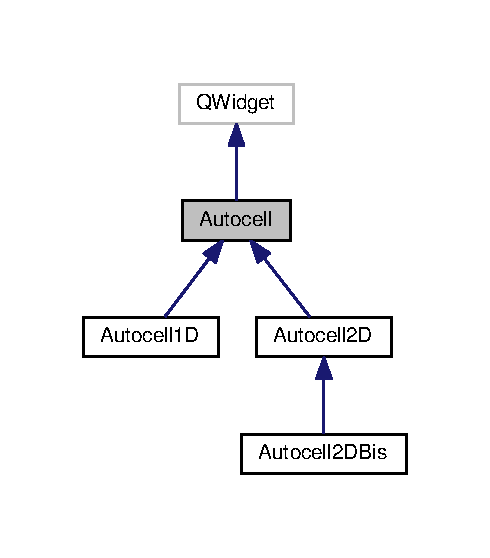
\includegraphics[width=235pt]{class_autocell__inherit__graph}
\end{center}
\end{figure}


Graphe de collaboration de Autocell\+:\nopagebreak
\begin{figure}[H]
\begin{center}
\leavevmode
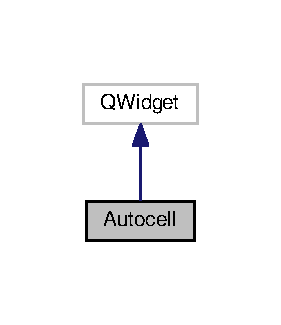
\includegraphics[width=135pt]{class_autocell__coll__graph}
\end{center}
\end{figure}
\subsection*{Connecteurs publics}
\begin{DoxyCompactItemize}
\item 
virtual void \hyperlink{class_autocell_afada0a9ee44f58fe4151a205337a6787}{cell\+Selected} (int a, int b)=0
\begin{DoxyCompactList}\small\item\em Change la couleur de la cellule selectionnée S\+L\+OT virtuel pur qui va réaliser une action à la selection (un click) d\textquotesingle{}une cellule. \end{DoxyCompactList}\end{DoxyCompactItemize}
\subsection*{Signaux}
\begin{DoxyCompactItemize}
\item 
void \hyperlink{class_autocell_a4a248ebfe4372c27a2d9b03c7b14ddf4}{end\+Sim} ()
\begin{DoxyCompactList}\small\item\em Signal de fin de simulation Signal envoyé à la fin de la simulation. \end{DoxyCompactList}\end{DoxyCompactItemize}
\subsection*{Fonctions membres publiques}
\begin{DoxyCompactItemize}
\item 
\hyperlink{class_autocell_a43f55284a9ec07e5d0619a87391d7cc7}{Autocell} (Q\+Widget $\ast$parent=nullptr, unsigned int etat=2)
\begin{DoxyCompactList}\small\item\em Constructeur de la classe \hyperlink{class_autocell}{Autocell}. \end{DoxyCompactList}\item 
virtual \hyperlink{class_autocell_acdb5335402dda348cc1e0a62e47418fe}{$\sim$\+Autocell} ()
\begin{DoxyCompactList}\small\item\em Destructeur virtuel de la classe \hyperlink{class_autocell}{Autocell}. \end{DoxyCompactList}\item 
void \hyperlink{class_autocell_a62154f66156d8abbde2dab84cc2b6b5d}{set\+Nb\+Etat} (unsigned int e)
\begin{DoxyCompactList}\small\item\em change le nombre d\textquotesingle{}état que peut prendre une cellule \end{DoxyCompactList}\item 
void \hyperlink{class_autocell_a8e1fab78b4369eceedad58ddee63ae78}{set\+Taille} (unsigned int t)
\begin{DoxyCompactList}\small\item\em change la taille des cellules \end{DoxyCompactList}\item 
void \hyperlink{class_autocell_ac1dd89aa8d881471b06802b2d780474a}{set\+Couleur} (std\+::vector$<$ std\+::string $>$ c)
\begin{DoxyCompactList}\small\item\em change la liste de couleur \end{DoxyCompactList}\item 
void \hyperlink{class_autocell_a5f449aec7927c7225ff22857d92e970d}{set\+Speed} (unsigned int s)
\begin{DoxyCompactList}\small\item\em change le delai \end{DoxyCompactList}\item 
void \hyperlink{class_autocell_af8ec313790f53cf4a3abbc688c2b307d}{set\+Continu} (bool a)
\begin{DoxyCompactList}\small\item\em change le mode de lecture de l\textquotesingle{}autocell \end{DoxyCompactList}\item 
unsigned int \hyperlink{class_autocell_a342d76cd9ff9ee3b9942a7917c12a435}{get\+Nb\+Etat} () const 
\begin{DoxyCompactList}\small\item\em accesseur Lecture \end{DoxyCompactList}\item 
unsigned int \hyperlink{class_autocell_af4649cfcee8d1eb6250de48110d2dda0}{get\+Taille} () const 
\begin{DoxyCompactList}\small\item\em accesseur Lecture \end{DoxyCompactList}\item 
unsigned int \hyperlink{class_autocell_af95bce9bd555eee6e38752a639265799}{get\+Largeur} () const 
\begin{DoxyCompactList}\small\item\em accesseur Lecture \end{DoxyCompactList}\item 
unsigned int \hyperlink{class_autocell_a6211b452c915737d2165dc7aeb7c31ba}{get\+Hauteur} () const 
\begin{DoxyCompactList}\small\item\em accesseur Lecture \end{DoxyCompactList}\item 
void \hyperlink{class_autocell_a8644ce5042e0849ebe0b0f045eed18a0}{set\+Hauteur} (unsigned int h)
\begin{DoxyCompactList}\small\item\em accesseur en écriture change la hauteur et ajuste la taille de la fenetre grâce à la méthode virtuelle pure \hyperlink{class_autocell_a060d956fa55ae3871081b3ecb949689f}{adjust\+Taille()} \end{DoxyCompactList}\item 
virtual void \hyperlink{class_autocell_a73af052faee8acf25c6f91aba3493004}{set\+Largeur} (unsigned int l)
\begin{DoxyCompactList}\small\item\em accesseur en écriture change la largeur et ajuste la taille de la fenetre grâce à la méthode virtuelle pure \hyperlink{class_autocell_a060d956fa55ae3871081b3ecb949689f}{adjust\+Taille()} \end{DoxyCompactList}\item 
virtual void \hyperlink{class_autocell_a83fb2030039bcddc40ee72f44ac38e63}{run\+Sim} ()=0
\begin{DoxyCompactList}\small\item\em Lance la simulation méthode virtuelle pure qui va permettre de lancer une simulation en fonction de l\textquotesingle{}automate. \end{DoxyCompactList}\item 
virtual void \hyperlink{class_autocell_abffbd1e2026f04e489a03cc9bc0c28f4}{clear} ()=0
\begin{DoxyCompactList}\small\item\em nettoie l\textquotesingle{}autocell méthode virtuelle pure qui va permettre de réinitialiser l\textquotesingle{}autocell \end{DoxyCompactList}\item 
virtual void \hyperlink{class_autocell_a060d956fa55ae3871081b3ecb949689f}{adjust\+Taille} ()=0
\begin{DoxyCompactList}\small\item\em ajuste l\textquotesingle{}autocell méthode virtuelle pure qui va permettre de d\textquotesingle{}ajuster l\textquotesingle{}autocelle en fonction de la largeur, hauteur et taille \end{DoxyCompactList}\item 
virtual void \hyperlink{class_autocell_ac505c956de1d90a48e2d3558bdf97253}{init} ()=0
\begin{DoxyCompactList}\small\item\em Génère une grille de départ méthode virtuelle pure qui va générer aléatoirement un état initiale pour l\textquotesingle{}autocell. \end{DoxyCompactList}\item 
virtual void \hyperlink{class_autocell_aa1e1870af0142596a9a81afe7f300a11}{init\+Sym} ()=0
\begin{DoxyCompactList}\small\item\em Génère une grille de départ symétrique méthode virtuelle pure qui va générer aléatoirement un état initiale symétrique par rapport à l\textquotesingle{}axe Y pour l\textquotesingle{}autocell. \end{DoxyCompactList}\end{DoxyCompactItemize}
\subsection*{Attributs protégés}
\begin{DoxyCompactItemize}
\item 
int \hyperlink{class_autocell_abcfd3af5e49b6a5b4538fb22a5f06d81}{taille} =17
\item 
unsigned int \hyperlink{class_autocell_a35a3592704f2fe987c846017b0fc83b2}{nb\+Etat}
\item 
unsigned int \hyperlink{class_autocell_a52291657adce98a0443559a5cd2e0c0b}{speed} =100
\item 
std\+::vector$<$ std\+::string $>$ \hyperlink{class_autocell_a42cb133bcf58ca2f0e797d938fb79cc5}{couleur}
\item 
int \hyperlink{class_autocell_a30f72e08777d91ecdd047ff5fa9b718f}{hauteur} =20
\item 
int \hyperlink{class_autocell_a7f7e3075befc2cae857ddbb9c4643ab7}{largeur} = 15
\item 
bool \hyperlink{class_autocell_acd28f9a1e0654c9c365923828924b78a}{continu} = true
\end{DoxyCompactItemize}


\subsection{Description détaillée}
Classe abstraite. La classe généralise un \hyperlink{class_autocell}{Autocell} et définie les méthodes virtuelles qui devront être présente et définie dans chaque \hyperlink{class_autocell}{Autocell}. La fenetre principale va alors mettre en action le polymorphisme, permettant alors de lancer, arrêter... n\textquotesingle{}importe quel \hyperlink{class_autocell}{Autocell}. 

\subsection{Documentation des constructeurs et destructeur}
\index{Autocell@{Autocell}!Autocell@{Autocell}}
\index{Autocell@{Autocell}!Autocell@{Autocell}}
\subsubsection[{\texorpdfstring{Autocell(\+Q\+Widget $\ast$parent=nullptr, unsigned int etat=2)}{Autocell(QWidget *parent=nullptr, unsigned int etat=2)}}]{\setlength{\rightskip}{0pt plus 5cm}Autocell\+::\+Autocell (
\begin{DoxyParamCaption}
\item[{Q\+Widget $\ast$}]{parent = {\ttfamily nullptr}, }
\item[{unsigned int}]{etat = {\ttfamily 2}}
\end{DoxyParamCaption}
)\hspace{0.3cm}{\ttfamily [inline]}}\hypertarget{class_autocell_a43f55284a9ec07e5d0619a87391d7cc7}{}\label{class_autocell_a43f55284a9ec07e5d0619a87391d7cc7}


Constructeur de la classe \hyperlink{class_autocell}{Autocell}. 


\begin{DoxyParams}{Paramètres}
{\em etat} & nombre d\textquotesingle{}états que peut prendre chaque cellule (2 par défaut)\+: unsigned int \\
\hline
\end{DoxyParams}
\index{Autocell@{Autocell}!````~Autocell@{$\sim$\+Autocell}}
\index{````~Autocell@{$\sim$\+Autocell}!Autocell@{Autocell}}
\subsubsection[{\texorpdfstring{$\sim$\+Autocell()}{~Autocell()}}]{\setlength{\rightskip}{0pt plus 5cm}virtual Autocell\+::$\sim$\+Autocell (
\begin{DoxyParamCaption}
{}
\end{DoxyParamCaption}
)\hspace{0.3cm}{\ttfamily [inline]}, {\ttfamily [virtual]}}\hypertarget{class_autocell_acdb5335402dda348cc1e0a62e47418fe}{}\label{class_autocell_acdb5335402dda348cc1e0a62e47418fe}


Destructeur virtuel de la classe \hyperlink{class_autocell}{Autocell}. 



\subsection{Documentation des fonctions membres}
\index{Autocell@{Autocell}!adjust\+Taille@{adjust\+Taille}}
\index{adjust\+Taille@{adjust\+Taille}!Autocell@{Autocell}}
\subsubsection[{\texorpdfstring{adjust\+Taille()=0}{adjustTaille()=0}}]{\setlength{\rightskip}{0pt plus 5cm}virtual void Autocell\+::adjust\+Taille (
\begin{DoxyParamCaption}
{}
\end{DoxyParamCaption}
)\hspace{0.3cm}{\ttfamily [pure virtual]}}\hypertarget{class_autocell_a060d956fa55ae3871081b3ecb949689f}{}\label{class_autocell_a060d956fa55ae3871081b3ecb949689f}


ajuste l\textquotesingle{}autocell méthode virtuelle pure qui va permettre de d\textquotesingle{}ajuster l\textquotesingle{}autocelle en fonction de la largeur, hauteur et taille 



Implémenté dans \hyperlink{class_autocell2_d_a76ab804bc939ebe1957dd2ba3ea93803}{Autocell2D}, et \hyperlink{class_autocell1_d_ade60b5de205e8890b608baa7b7c4d186}{Autocell1D}.

\index{Autocell@{Autocell}!cell\+Selected@{cell\+Selected}}
\index{cell\+Selected@{cell\+Selected}!Autocell@{Autocell}}
\subsubsection[{\texorpdfstring{cell\+Selected}{cellSelected}}]{\setlength{\rightskip}{0pt plus 5cm}virtual void Autocell\+::cell\+Selected (
\begin{DoxyParamCaption}
\item[{int}]{a, }
\item[{int}]{b}
\end{DoxyParamCaption}
)\hspace{0.3cm}{\ttfamily [pure virtual]}, {\ttfamily [slot]}}\hypertarget{class_autocell_afada0a9ee44f58fe4151a205337a6787}{}\label{class_autocell_afada0a9ee44f58fe4151a205337a6787}


Change la couleur de la cellule selectionnée S\+L\+OT virtuel pur qui va réaliser une action à la selection (un click) d\textquotesingle{}une cellule. 

\index{Autocell@{Autocell}!clear@{clear}}
\index{clear@{clear}!Autocell@{Autocell}}
\subsubsection[{\texorpdfstring{clear()=0}{clear()=0}}]{\setlength{\rightskip}{0pt plus 5cm}virtual void Autocell\+::clear (
\begin{DoxyParamCaption}
{}
\end{DoxyParamCaption}
)\hspace{0.3cm}{\ttfamily [pure virtual]}}\hypertarget{class_autocell_abffbd1e2026f04e489a03cc9bc0c28f4}{}\label{class_autocell_abffbd1e2026f04e489a03cc9bc0c28f4}


nettoie l\textquotesingle{}autocell méthode virtuelle pure qui va permettre de réinitialiser l\textquotesingle{}autocell 



Implémenté dans \hyperlink{class_autocell1_d_a711408c00cac1a00112ce8a72eab5b48}{Autocell1D}.

\index{Autocell@{Autocell}!end\+Sim@{end\+Sim}}
\index{end\+Sim@{end\+Sim}!Autocell@{Autocell}}
\subsubsection[{\texorpdfstring{end\+Sim}{endSim}}]{\setlength{\rightskip}{0pt plus 5cm}void Autocell\+::end\+Sim (
\begin{DoxyParamCaption}
{}
\end{DoxyParamCaption}
)\hspace{0.3cm}{\ttfamily [signal]}}\hypertarget{class_autocell_a4a248ebfe4372c27a2d9b03c7b14ddf4}{}\label{class_autocell_a4a248ebfe4372c27a2d9b03c7b14ddf4}


Signal de fin de simulation Signal envoyé à la fin de la simulation. 

\index{Autocell@{Autocell}!get\+Hauteur@{get\+Hauteur}}
\index{get\+Hauteur@{get\+Hauteur}!Autocell@{Autocell}}
\subsubsection[{\texorpdfstring{get\+Hauteur() const }{getHauteur() const }}]{\setlength{\rightskip}{0pt plus 5cm}unsigned int Autocell\+::get\+Hauteur (
\begin{DoxyParamCaption}
{}
\end{DoxyParamCaption}
) const\hspace{0.3cm}{\ttfamily [inline]}}\hypertarget{class_autocell_a6211b452c915737d2165dc7aeb7c31ba}{}\label{class_autocell_a6211b452c915737d2165dc7aeb7c31ba}


accesseur Lecture 

\begin{DoxyReturn}{Renvoie}
retourne la hauteur 
\end{DoxyReturn}
\index{Autocell@{Autocell}!get\+Largeur@{get\+Largeur}}
\index{get\+Largeur@{get\+Largeur}!Autocell@{Autocell}}
\subsubsection[{\texorpdfstring{get\+Largeur() const }{getLargeur() const }}]{\setlength{\rightskip}{0pt plus 5cm}unsigned int Autocell\+::get\+Largeur (
\begin{DoxyParamCaption}
{}
\end{DoxyParamCaption}
) const\hspace{0.3cm}{\ttfamily [inline]}}\hypertarget{class_autocell_af95bce9bd555eee6e38752a639265799}{}\label{class_autocell_af95bce9bd555eee6e38752a639265799}


accesseur Lecture 

\begin{DoxyReturn}{Renvoie}
retourne la largeur 
\end{DoxyReturn}
\index{Autocell@{Autocell}!get\+Nb\+Etat@{get\+Nb\+Etat}}
\index{get\+Nb\+Etat@{get\+Nb\+Etat}!Autocell@{Autocell}}
\subsubsection[{\texorpdfstring{get\+Nb\+Etat() const }{getNbEtat() const }}]{\setlength{\rightskip}{0pt plus 5cm}unsigned int Autocell\+::get\+Nb\+Etat (
\begin{DoxyParamCaption}
{}
\end{DoxyParamCaption}
) const\hspace{0.3cm}{\ttfamily [inline]}}\hypertarget{class_autocell_a342d76cd9ff9ee3b9942a7917c12a435}{}\label{class_autocell_a342d76cd9ff9ee3b9942a7917c12a435}


accesseur Lecture 

\begin{DoxyReturn}{Renvoie}
retourne le nombre d\textquotesingle{}états 
\end{DoxyReturn}
\index{Autocell@{Autocell}!get\+Taille@{get\+Taille}}
\index{get\+Taille@{get\+Taille}!Autocell@{Autocell}}
\subsubsection[{\texorpdfstring{get\+Taille() const }{getTaille() const }}]{\setlength{\rightskip}{0pt plus 5cm}unsigned int Autocell\+::get\+Taille (
\begin{DoxyParamCaption}
{}
\end{DoxyParamCaption}
) const\hspace{0.3cm}{\ttfamily [inline]}}\hypertarget{class_autocell_af4649cfcee8d1eb6250de48110d2dda0}{}\label{class_autocell_af4649cfcee8d1eb6250de48110d2dda0}


accesseur Lecture 

\begin{DoxyReturn}{Renvoie}
retourne la taille 
\end{DoxyReturn}
\index{Autocell@{Autocell}!init@{init}}
\index{init@{init}!Autocell@{Autocell}}
\subsubsection[{\texorpdfstring{init()=0}{init()=0}}]{\setlength{\rightskip}{0pt plus 5cm}virtual void Autocell\+::init (
\begin{DoxyParamCaption}
{}
\end{DoxyParamCaption}
)\hspace{0.3cm}{\ttfamily [pure virtual]}}\hypertarget{class_autocell_ac505c956de1d90a48e2d3558bdf97253}{}\label{class_autocell_ac505c956de1d90a48e2d3558bdf97253}


Génère une grille de départ méthode virtuelle pure qui va générer aléatoirement un état initiale pour l\textquotesingle{}autocell. 



Implémenté dans \hyperlink{class_autocell2_d_a9380918c9f11ff223223672685b2cdb7}{Autocell2D}, et \hyperlink{class_autocell1_d_a53c95905c3b33bf49a92b64f39ec2c29}{Autocell1D}.

\index{Autocell@{Autocell}!init\+Sym@{init\+Sym}}
\index{init\+Sym@{init\+Sym}!Autocell@{Autocell}}
\subsubsection[{\texorpdfstring{init\+Sym()=0}{initSym()=0}}]{\setlength{\rightskip}{0pt plus 5cm}virtual void Autocell\+::init\+Sym (
\begin{DoxyParamCaption}
{}
\end{DoxyParamCaption}
)\hspace{0.3cm}{\ttfamily [pure virtual]}}\hypertarget{class_autocell_aa1e1870af0142596a9a81afe7f300a11}{}\label{class_autocell_aa1e1870af0142596a9a81afe7f300a11}


Génère une grille de départ symétrique méthode virtuelle pure qui va générer aléatoirement un état initiale symétrique par rapport à l\textquotesingle{}axe Y pour l\textquotesingle{}autocell. 



Implémenté dans \hyperlink{class_autocell2_d_acd5f269beafa7f81ff57d6f05013892e}{Autocell2D}, et \hyperlink{class_autocell1_d_a5ad8a1b903cca1cce5965d22039b6e04}{Autocell1D}.

\index{Autocell@{Autocell}!run\+Sim@{run\+Sim}}
\index{run\+Sim@{run\+Sim}!Autocell@{Autocell}}
\subsubsection[{\texorpdfstring{run\+Sim()=0}{runSim()=0}}]{\setlength{\rightskip}{0pt plus 5cm}virtual void Autocell\+::run\+Sim (
\begin{DoxyParamCaption}
{}
\end{DoxyParamCaption}
)\hspace{0.3cm}{\ttfamily [pure virtual]}}\hypertarget{class_autocell_a83fb2030039bcddc40ee72f44ac38e63}{}\label{class_autocell_a83fb2030039bcddc40ee72f44ac38e63}


Lance la simulation méthode virtuelle pure qui va permettre de lancer une simulation en fonction de l\textquotesingle{}automate. 



Implémenté dans \hyperlink{class_autocell1_d_a4793eae53adcca32290621c45a76260c}{Autocell1D}.

\index{Autocell@{Autocell}!set\+Continu@{set\+Continu}}
\index{set\+Continu@{set\+Continu}!Autocell@{Autocell}}
\subsubsection[{\texorpdfstring{set\+Continu(bool a)}{setContinu(bool a)}}]{\setlength{\rightskip}{0pt plus 5cm}void Autocell\+::set\+Continu (
\begin{DoxyParamCaption}
\item[{bool}]{a}
\end{DoxyParamCaption}
)\hspace{0.3cm}{\ttfamily [inline]}}\hypertarget{class_autocell_af8ec313790f53cf4a3abbc688c2b307d}{}\label{class_autocell_af8ec313790f53cf4a3abbc688c2b307d}


change le mode de lecture de l\textquotesingle{}autocell 


\begin{DoxyParams}{Paramètres}
{\em a} & \+: mode de lecture\+: bool \\
\hline
\end{DoxyParams}
\index{Autocell@{Autocell}!set\+Couleur@{set\+Couleur}}
\index{set\+Couleur@{set\+Couleur}!Autocell@{Autocell}}
\subsubsection[{\texorpdfstring{set\+Couleur(std\+::vector$<$ std\+::string $>$ c)}{setCouleur(std::vector< std::string > c)}}]{\setlength{\rightskip}{0pt plus 5cm}void Autocell\+::set\+Couleur (
\begin{DoxyParamCaption}
\item[{std\+::vector$<$ std\+::string $>$}]{c}
\end{DoxyParamCaption}
)\hspace{0.3cm}{\ttfamily [inline]}}\hypertarget{class_autocell_ac1dd89aa8d881471b06802b2d780474a}{}\label{class_autocell_ac1dd89aa8d881471b06802b2d780474a}


change la liste de couleur 


\begin{DoxyParams}{Paramètres}
{\em c} & \+: nouvelle liste de couleur\+: std\+::vector$<$std\+::string$>$ \\
\hline
\end{DoxyParams}
\index{Autocell@{Autocell}!set\+Hauteur@{set\+Hauteur}}
\index{set\+Hauteur@{set\+Hauteur}!Autocell@{Autocell}}
\subsubsection[{\texorpdfstring{set\+Hauteur(unsigned int h)}{setHauteur(unsigned int h)}}]{\setlength{\rightskip}{0pt plus 5cm}void Autocell\+::set\+Hauteur (
\begin{DoxyParamCaption}
\item[{unsigned int}]{h}
\end{DoxyParamCaption}
)\hspace{0.3cm}{\ttfamily [inline]}}\hypertarget{class_autocell_a8644ce5042e0849ebe0b0f045eed18a0}{}\label{class_autocell_a8644ce5042e0849ebe0b0f045eed18a0}


accesseur en écriture change la hauteur et ajuste la taille de la fenetre grâce à la méthode virtuelle pure \hyperlink{class_autocell_a060d956fa55ae3871081b3ecb949689f}{adjust\+Taille()} 


\begin{DoxyParams}{Paramètres}
{\em h} & \+: nouvelle hauteur\+: unsigned int \\
\hline
\end{DoxyParams}
\index{Autocell@{Autocell}!set\+Largeur@{set\+Largeur}}
\index{set\+Largeur@{set\+Largeur}!Autocell@{Autocell}}
\subsubsection[{\texorpdfstring{set\+Largeur(unsigned int l)}{setLargeur(unsigned int l)}}]{\setlength{\rightskip}{0pt plus 5cm}virtual void Autocell\+::set\+Largeur (
\begin{DoxyParamCaption}
\item[{unsigned int}]{l}
\end{DoxyParamCaption}
)\hspace{0.3cm}{\ttfamily [inline]}, {\ttfamily [virtual]}}\hypertarget{class_autocell_a73af052faee8acf25c6f91aba3493004}{}\label{class_autocell_a73af052faee8acf25c6f91aba3493004}


accesseur en écriture change la largeur et ajuste la taille de la fenetre grâce à la méthode virtuelle pure \hyperlink{class_autocell_a060d956fa55ae3871081b3ecb949689f}{adjust\+Taille()} 


\begin{DoxyParams}{Paramètres}
{\em l} & \+: nouvelle largeur\+:unsigned int \\
\hline
\end{DoxyParams}
\index{Autocell@{Autocell}!set\+Nb\+Etat@{set\+Nb\+Etat}}
\index{set\+Nb\+Etat@{set\+Nb\+Etat}!Autocell@{Autocell}}
\subsubsection[{\texorpdfstring{set\+Nb\+Etat(unsigned int e)}{setNbEtat(unsigned int e)}}]{\setlength{\rightskip}{0pt plus 5cm}void Autocell\+::set\+Nb\+Etat (
\begin{DoxyParamCaption}
\item[{unsigned int}]{e}
\end{DoxyParamCaption}
)\hspace{0.3cm}{\ttfamily [inline]}}\hypertarget{class_autocell_a62154f66156d8abbde2dab84cc2b6b5d}{}\label{class_autocell_a62154f66156d8abbde2dab84cc2b6b5d}


change le nombre d\textquotesingle{}état que peut prendre une cellule 


\begin{DoxyParams}{Paramètres}
{\em e} & \+: nouveau nombre d\textquotesingle{}état\+: unsigned int \\
\hline
\end{DoxyParams}
\index{Autocell@{Autocell}!set\+Speed@{set\+Speed}}
\index{set\+Speed@{set\+Speed}!Autocell@{Autocell}}
\subsubsection[{\texorpdfstring{set\+Speed(unsigned int s)}{setSpeed(unsigned int s)}}]{\setlength{\rightskip}{0pt plus 5cm}void Autocell\+::set\+Speed (
\begin{DoxyParamCaption}
\item[{unsigned int}]{s}
\end{DoxyParamCaption}
)\hspace{0.3cm}{\ttfamily [inline]}}\hypertarget{class_autocell_a5f449aec7927c7225ff22857d92e970d}{}\label{class_autocell_a5f449aec7927c7225ff22857d92e970d}


change le delai 


\begin{DoxyParams}{Paramètres}
{\em s} & \+: nouveau délai\+: unsigned int \\
\hline
\end{DoxyParams}
\index{Autocell@{Autocell}!set\+Taille@{set\+Taille}}
\index{set\+Taille@{set\+Taille}!Autocell@{Autocell}}
\subsubsection[{\texorpdfstring{set\+Taille(unsigned int t)}{setTaille(unsigned int t)}}]{\setlength{\rightskip}{0pt plus 5cm}void Autocell\+::set\+Taille (
\begin{DoxyParamCaption}
\item[{unsigned int}]{t}
\end{DoxyParamCaption}
)\hspace{0.3cm}{\ttfamily [inline]}}\hypertarget{class_autocell_a8e1fab78b4369eceedad58ddee63ae78}{}\label{class_autocell_a8e1fab78b4369eceedad58ddee63ae78}


change la taille des cellules 


\begin{DoxyParams}{Paramètres}
{\em t} & \+:nouvelle taille\+: unsigned int \\
\hline
\end{DoxyParams}


\subsection{Documentation des données membres}
\index{Autocell@{Autocell}!continu@{continu}}
\index{continu@{continu}!Autocell@{Autocell}}
\subsubsection[{\texorpdfstring{continu}{continu}}]{\setlength{\rightskip}{0pt plus 5cm}bool Autocell\+::continu = true\hspace{0.3cm}{\ttfamily [protected]}}\hypertarget{class_autocell_acd28f9a1e0654c9c365923828924b78a}{}\label{class_autocell_acd28f9a1e0654c9c365923828924b78a}
Mode de lecture \index{Autocell@{Autocell}!couleur@{couleur}}
\index{couleur@{couleur}!Autocell@{Autocell}}
\subsubsection[{\texorpdfstring{couleur}{couleur}}]{\setlength{\rightskip}{0pt plus 5cm}std\+::vector$<$std\+::string$>$ Autocell\+::couleur\hspace{0.3cm}{\ttfamily [protected]}}\hypertarget{class_autocell_a42cb133bcf58ca2f0e797d938fb79cc5}{}\label{class_autocell_a42cb133bcf58ca2f0e797d938fb79cc5}
liste des couleurs pour chaque état i \index{Autocell@{Autocell}!hauteur@{hauteur}}
\index{hauteur@{hauteur}!Autocell@{Autocell}}
\subsubsection[{\texorpdfstring{hauteur}{hauteur}}]{\setlength{\rightskip}{0pt plus 5cm}int Autocell\+::hauteur =20\hspace{0.3cm}{\ttfamily [protected]}}\hypertarget{class_autocell_a30f72e08777d91ecdd047ff5fa9b718f}{}\label{class_autocell_a30f72e08777d91ecdd047ff5fa9b718f}
hauteur de la grille(pour \hyperlink{class_autocell1_d}{Autocell1D} la hauteur représente le nombre de simulation) \index{Autocell@{Autocell}!largeur@{largeur}}
\index{largeur@{largeur}!Autocell@{Autocell}}
\subsubsection[{\texorpdfstring{largeur}{largeur}}]{\setlength{\rightskip}{0pt plus 5cm}int Autocell\+::largeur = 15\hspace{0.3cm}{\ttfamily [protected]}}\hypertarget{class_autocell_a7f7e3075befc2cae857ddbb9c4643ab7}{}\label{class_autocell_a7f7e3075befc2cae857ddbb9c4643ab7}
Largeur de la grille \index{Autocell@{Autocell}!nb\+Etat@{nb\+Etat}}
\index{nb\+Etat@{nb\+Etat}!Autocell@{Autocell}}
\subsubsection[{\texorpdfstring{nb\+Etat}{nbEtat}}]{\setlength{\rightskip}{0pt plus 5cm}unsigned int Autocell\+::nb\+Etat\hspace{0.3cm}{\ttfamily [protected]}}\hypertarget{class_autocell_a35a3592704f2fe987c846017b0fc83b2}{}\label{class_autocell_a35a3592704f2fe987c846017b0fc83b2}
Nombre d\textquotesingle{}état pour une cellule \index{Autocell@{Autocell}!speed@{speed}}
\index{speed@{speed}!Autocell@{Autocell}}
\subsubsection[{\texorpdfstring{speed}{speed}}]{\setlength{\rightskip}{0pt plus 5cm}unsigned int Autocell\+::speed =100\hspace{0.3cm}{\ttfamily [protected]}}\hypertarget{class_autocell_a52291657adce98a0443559a5cd2e0c0b}{}\label{class_autocell_a52291657adce98a0443559a5cd2e0c0b}
delai entre chaque simulation \index{Autocell@{Autocell}!taille@{taille}}
\index{taille@{taille}!Autocell@{Autocell}}
\subsubsection[{\texorpdfstring{taille}{taille}}]{\setlength{\rightskip}{0pt plus 5cm}int Autocell\+::taille =17\hspace{0.3cm}{\ttfamily [protected]}}\hypertarget{class_autocell_abcfd3af5e49b6a5b4538fb22a5f06d81}{}\label{class_autocell_abcfd3af5e49b6a5b4538fb22a5f06d81}
Taille d\textquotesingle{}une cellule 

La documentation de cette classe a été générée à partir des fichiers suivants \+:\begin{DoxyCompactItemize}
\item 
/home/thomaspaita/\+Bureau/info/\+L\+O21/\+L\+O21/\+Auto\+Cell/\hyperlink{autocell_8h}{autocell.\+h}\item 
/home/thomaspaita/\+Bureau/info/\+L\+O21/\+L\+O21/build-\/\+Auto\+Cell-\/\+Desktop-\/\+Debug/\hyperlink{moc__autocell_8cpp}{moc\+\_\+autocell.\+cpp}\end{DoxyCompactItemize}

\hypertarget{class_autocell1_d}{}\section{Référence de la classe Autocell1D}
\label{class_autocell1_d}\index{Autocell1D@{Autocell1D}}


Hérite de \hyperlink{class_autocell}{Autocell}. La classe \hyperlink{class_autocell1_d}{Autocell1D} permet de lancer des automates cellulaires à 1\+Dimensions (classe \hyperlink{class_automate1_d}{Automate1D} et \hyperlink{class_etat1_d}{Etat1D})  




{\ttfamily \#include $<$autocell.\+h$>$}



Graphe d\textquotesingle{}héritage de Autocell1D\+:
\nopagebreak
\begin{figure}[H]
\begin{center}
\leavevmode
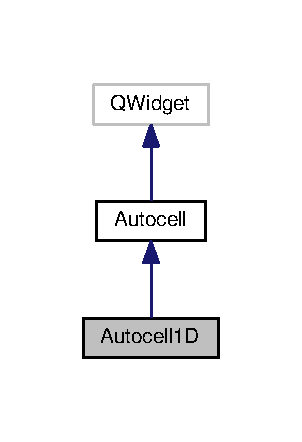
\includegraphics[width=145pt]{class_autocell1_d__inherit__graph}
\end{center}
\end{figure}


Graphe de collaboration de Autocell1D\+:
\nopagebreak
\begin{figure}[H]
\begin{center}
\leavevmode
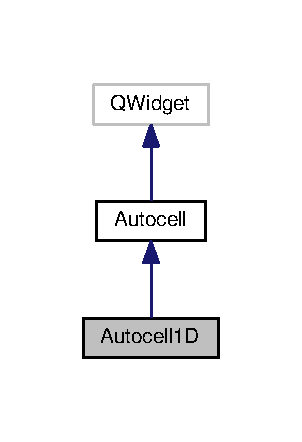
\includegraphics[width=145pt]{class_autocell1_d__coll__graph}
\end{center}
\end{figure}
\subsection*{Connecteurs publics}
\begin{DoxyCompactItemize}
\item 
virtual void \hyperlink{class_autocell1_d_ac38fb0d27778ecdff40628556956f64a}{cell\+Selected} (int a, int b)
\begin{DoxyCompactList}\small\item\em S\+L\+OT qui change la couleur d\textquotesingle{}une cellule (a,b) \end{DoxyCompactList}\end{DoxyCompactItemize}
\subsection*{Fonctions membres publiques}
\begin{DoxyCompactItemize}
\item 
\hyperlink{class_autocell1_d_a4a706f162ed7e0b81f55a3463e355c9c}{Autocell1D} (Q\+Widget $\ast$parent=nullptr)
\begin{DoxyCompactList}\small\item\em constructeur \end{DoxyCompactList}\item 
void \hyperlink{class_autocell1_d_a9591755409ac74ff5564d86af4236a28}{set\+Regle} (unsigned int r)
\begin{DoxyCompactList}\small\item\em change la règle \end{DoxyCompactList}\item 
void \hyperlink{class_autocell1_d_a624d426584e5dbc621416118f09ac528}{set\+Color} (Q\+String a)
\begin{DoxyCompactList}\small\item\em change la couleur \end{DoxyCompactList}\item 
const Q\+Table\+Widget $\ast$ \hyperlink{class_autocell1_d_af724076ad7bd4f512174d63394c89aba}{get\+\_\+depart} () const 
\begin{DoxyCompactList}\small\item\em retourne le départ \end{DoxyCompactList}\item 
void \hyperlink{class_autocell1_d_a4e7c5c216925849a0ba80ea94272b63e}{set\+Depart} (unsigned int i, Q\+String color)
\begin{DoxyCompactList}\small\item\em change la case i de l\textquotesingle{}état de départ dans l\textquotesingle{}attribut membre depart \end{DoxyCompactList}\item 
virtual void \hyperlink{class_autocell1_d_a4793eae53adcca32290621c45a76260c}{run\+Sim} ()
\begin{DoxyCompactList}\small\item\em Simule un automate1D construit un automate1D et un etat1D. \end{DoxyCompactList}\item 
virtual void \hyperlink{class_autocell1_d_ade60b5de205e8890b608baa7b7c4d186}{adjust\+Taille} ()
\begin{DoxyCompactList}\small\item\em ajuste la fenêtre ajuste la fenêtre en fonction de la largeur, hauteur et la taille \end{DoxyCompactList}\item 
virtual void \hyperlink{class_autocell1_d_a711408c00cac1a00112ce8a72eab5b48}{clear} ()
\begin{DoxyCompactList}\small\item\em nettoie l\textquotesingle{}autocell \end{DoxyCompactList}\item 
virtual void \hyperlink{class_autocell1_d_a53c95905c3b33bf49a92b64f39ec2c29}{init} ()
\begin{DoxyCompactList}\small\item\em initialise un état de départ pour l\textquotesingle{}attribut membre depart aléatoirement \end{DoxyCompactList}\item 
virtual void \hyperlink{class_autocell1_d_a5ad8a1b903cca1cce5965d22039b6e04}{init\+Sym} ()
\begin{DoxyCompactList}\small\item\em initialise un état de départ pour l\textquotesingle{}attribut membre depart symétriquement \end{DoxyCompactList}\end{DoxyCompactItemize}
\subsection*{Fonctions membres protégées}
\begin{DoxyCompactItemize}
\item 
void \hyperlink{class_autocell1_d_af7a137f43564c602e7503b34a232c4e0}{set\+Etat\+Depart} (int dim)
\begin{DoxyCompactList}\small\item\em initialise grille de départ méthode privée qui est utilisée dans le constructeur \end{DoxyCompactList}\end{DoxyCompactItemize}
\subsection*{Attributs protégés}
\begin{DoxyCompactItemize}
\item 
Q\+Grid\+Layout $\ast$ \hyperlink{class_autocell1_d_a7934db954892dc0efc12a961686a75c0}{layout}
\item 
Q\+Table\+Widget $\ast$ \hyperlink{class_autocell1_d_a7bd65a39691f86e179bcb0466e7e38c2}{depart}
\item 
Q\+Table\+Widget $\ast$ \hyperlink{class_autocell1_d_aed4038c48d9cc0a841e6f565d4cd792c}{etats} = nullptr
\item 
unsigned int \hyperlink{class_autocell1_d_ae28c4a70102bd5e08a2414d27b20bb47}{regle} =0
\end{DoxyCompactItemize}
\subsection*{Membres hérités additionnels}


\subsection{Description détaillée}
Hérite de \hyperlink{class_autocell}{Autocell}. La classe \hyperlink{class_autocell1_d}{Autocell1D} permet de lancer des automates cellulaires à 1\+Dimensions (classe \hyperlink{class_automate1_d}{Automate1D} et \hyperlink{class_etat1_d}{Etat1D}) 

\subsection{Documentation des constructeurs et destructeur}
\index{Autocell1D@{Autocell1D}!Autocell1D@{Autocell1D}}
\index{Autocell1D@{Autocell1D}!Autocell1D@{Autocell1D}}
\subsubsection[{\texorpdfstring{Autocell1\+D(\+Q\+Widget $\ast$parent=nullptr)}{Autocell1D(QWidget *parent=nullptr)}}]{\setlength{\rightskip}{0pt plus 5cm}Autocell1\+D\+::\+Autocell1D (
\begin{DoxyParamCaption}
\item[{Q\+Widget $\ast$}]{parent = {\ttfamily nullptr}}
\end{DoxyParamCaption}
)\hspace{0.3cm}{\ttfamily [explicit]}}\hypertarget{class_autocell1_d_a4a706f162ed7e0b81f55a3463e355c9c}{}\label{class_autocell1_d_a4a706f162ed7e0b81f55a3463e355c9c}


constructeur 



\subsection{Documentation des fonctions membres}
\index{Autocell1D@{Autocell1D}!adjust\+Taille@{adjust\+Taille}}
\index{adjust\+Taille@{adjust\+Taille}!Autocell1D@{Autocell1D}}
\subsubsection[{\texorpdfstring{adjust\+Taille()}{adjustTaille()}}]{\setlength{\rightskip}{0pt plus 5cm}void Autocell1\+D\+::adjust\+Taille (
\begin{DoxyParamCaption}
{}
\end{DoxyParamCaption}
)\hspace{0.3cm}{\ttfamily [virtual]}}\hypertarget{class_autocell1_d_ade60b5de205e8890b608baa7b7c4d186}{}\label{class_autocell1_d_ade60b5de205e8890b608baa7b7c4d186}


ajuste la fenêtre ajuste la fenêtre en fonction de la largeur, hauteur et la taille 



Implémente \hyperlink{class_autocell_a060d956fa55ae3871081b3ecb949689f}{Autocell}.

\index{Autocell1D@{Autocell1D}!cell\+Selected@{cell\+Selected}}
\index{cell\+Selected@{cell\+Selected}!Autocell1D@{Autocell1D}}
\subsubsection[{\texorpdfstring{cell\+Selected}{cellSelected}}]{\setlength{\rightskip}{0pt plus 5cm}void Autocell1\+D\+::cell\+Selected (
\begin{DoxyParamCaption}
\item[{int}]{a, }
\item[{int}]{b}
\end{DoxyParamCaption}
)\hspace{0.3cm}{\ttfamily [virtual]}, {\ttfamily [slot]}}\hypertarget{class_autocell1_d_ac38fb0d27778ecdff40628556956f64a}{}\label{class_autocell1_d_ac38fb0d27778ecdff40628556956f64a}


S\+L\+OT qui change la couleur d\textquotesingle{}une cellule (a,b) 


\begin{DoxyParams}{Paramètres}
{\em ligne\+:int} & \\
\hline
{\em colonne} & int \\
\hline
\end{DoxyParams}
\index{Autocell1D@{Autocell1D}!clear@{clear}}
\index{clear@{clear}!Autocell1D@{Autocell1D}}
\subsubsection[{\texorpdfstring{clear()}{clear()}}]{\setlength{\rightskip}{0pt plus 5cm}void Autocell1\+D\+::clear (
\begin{DoxyParamCaption}
{}
\end{DoxyParamCaption}
)\hspace{0.3cm}{\ttfamily [virtual]}}\hypertarget{class_autocell1_d_a711408c00cac1a00112ce8a72eab5b48}{}\label{class_autocell1_d_a711408c00cac1a00112ce8a72eab5b48}


nettoie l\textquotesingle{}autocell 



Implémente \hyperlink{class_autocell_abffbd1e2026f04e489a03cc9bc0c28f4}{Autocell}.

\index{Autocell1D@{Autocell1D}!get\+\_\+depart@{get\+\_\+depart}}
\index{get\+\_\+depart@{get\+\_\+depart}!Autocell1D@{Autocell1D}}
\subsubsection[{\texorpdfstring{get\+\_\+depart() const }{get_depart() const }}]{\setlength{\rightskip}{0pt plus 5cm}const Q\+Table\+Widget$\ast$ Autocell1\+D\+::get\+\_\+depart (
\begin{DoxyParamCaption}
{}
\end{DoxyParamCaption}
) const\hspace{0.3cm}{\ttfamily [inline]}}\hypertarget{class_autocell1_d_af724076ad7bd4f512174d63394c89aba}{}\label{class_autocell1_d_af724076ad7bd4f512174d63394c89aba}


retourne le départ 

\begin{DoxyReturn}{Renvoie}
const Q\+Table\+Widget$\ast$ 
\end{DoxyReturn}
\index{Autocell1D@{Autocell1D}!init@{init}}
\index{init@{init}!Autocell1D@{Autocell1D}}
\subsubsection[{\texorpdfstring{init()}{init()}}]{\setlength{\rightskip}{0pt plus 5cm}void Autocell1\+D\+::init (
\begin{DoxyParamCaption}
{}
\end{DoxyParamCaption}
)\hspace{0.3cm}{\ttfamily [virtual]}}\hypertarget{class_autocell1_d_a53c95905c3b33bf49a92b64f39ec2c29}{}\label{class_autocell1_d_a53c95905c3b33bf49a92b64f39ec2c29}


initialise un état de départ pour l\textquotesingle{}attribut membre depart aléatoirement 



Implémente \hyperlink{class_autocell_ac505c956de1d90a48e2d3558bdf97253}{Autocell}.

\index{Autocell1D@{Autocell1D}!init\+Sym@{init\+Sym}}
\index{init\+Sym@{init\+Sym}!Autocell1D@{Autocell1D}}
\subsubsection[{\texorpdfstring{init\+Sym()}{initSym()}}]{\setlength{\rightskip}{0pt plus 5cm}void Autocell1\+D\+::init\+Sym (
\begin{DoxyParamCaption}
{}
\end{DoxyParamCaption}
)\hspace{0.3cm}{\ttfamily [virtual]}}\hypertarget{class_autocell1_d_a5ad8a1b903cca1cce5965d22039b6e04}{}\label{class_autocell1_d_a5ad8a1b903cca1cce5965d22039b6e04}


initialise un état de départ pour l\textquotesingle{}attribut membre depart symétriquement 



Implémente \hyperlink{class_autocell_aa1e1870af0142596a9a81afe7f300a11}{Autocell}.

\index{Autocell1D@{Autocell1D}!run\+Sim@{run\+Sim}}
\index{run\+Sim@{run\+Sim}!Autocell1D@{Autocell1D}}
\subsubsection[{\texorpdfstring{run\+Sim()}{runSim()}}]{\setlength{\rightskip}{0pt plus 5cm}void Autocell1\+D\+::run\+Sim (
\begin{DoxyParamCaption}
{}
\end{DoxyParamCaption}
)\hspace{0.3cm}{\ttfamily [virtual]}}\hypertarget{class_autocell1_d_a4793eae53adcca32290621c45a76260c}{}\label{class_autocell1_d_a4793eae53adcca32290621c45a76260c}


Simule un automate1D construit un automate1D et un etat1D. 



Implémente \hyperlink{class_autocell_a83fb2030039bcddc40ee72f44ac38e63}{Autocell}.

\index{Autocell1D@{Autocell1D}!set\+Color@{set\+Color}}
\index{set\+Color@{set\+Color}!Autocell1D@{Autocell1D}}
\subsubsection[{\texorpdfstring{set\+Color(\+Q\+String a)}{setColor(QString a)}}]{\setlength{\rightskip}{0pt plus 5cm}void Autocell1\+D\+::set\+Color (
\begin{DoxyParamCaption}
\item[{Q\+String}]{a}
\end{DoxyParamCaption}
)}\hypertarget{class_autocell1_d_a624d426584e5dbc621416118f09ac528}{}\label{class_autocell1_d_a624d426584e5dbc621416118f09ac528}


change la couleur 


\begin{DoxyParams}{Paramètres}
{\em a} & \+: nouvelle couleur\+: Q\+String \\
\hline
\end{DoxyParams}
\index{Autocell1D@{Autocell1D}!set\+Depart@{set\+Depart}}
\index{set\+Depart@{set\+Depart}!Autocell1D@{Autocell1D}}
\subsubsection[{\texorpdfstring{set\+Depart(unsigned int i, Q\+String color)}{setDepart(unsigned int i, QString color)}}]{\setlength{\rightskip}{0pt plus 5cm}void Autocell1\+D\+::set\+Depart (
\begin{DoxyParamCaption}
\item[{unsigned int}]{i, }
\item[{Q\+String}]{color}
\end{DoxyParamCaption}
)\hspace{0.3cm}{\ttfamily [inline]}}\hypertarget{class_autocell1_d_a4e7c5c216925849a0ba80ea94272b63e}{}\label{class_autocell1_d_a4e7c5c216925849a0ba80ea94272b63e}


change la case i de l\textquotesingle{}état de départ dans l\textquotesingle{}attribut membre depart 


\begin{DoxyParams}{Paramètres}
{\em i} & \+: indice\+: unsigned int \\
\hline
{\em color} & \+: couleur de la case\+: Q\+String \\
\hline
\end{DoxyParams}
\index{Autocell1D@{Autocell1D}!set\+Etat\+Depart@{set\+Etat\+Depart}}
\index{set\+Etat\+Depart@{set\+Etat\+Depart}!Autocell1D@{Autocell1D}}
\subsubsection[{\texorpdfstring{set\+Etat\+Depart(int dim)}{setEtatDepart(int dim)}}]{\setlength{\rightskip}{0pt plus 5cm}void Autocell1\+D\+::set\+Etat\+Depart (
\begin{DoxyParamCaption}
\item[{int}]{dim}
\end{DoxyParamCaption}
)\hspace{0.3cm}{\ttfamily [protected]}}\hypertarget{class_autocell1_d_af7a137f43564c602e7503b34a232c4e0}{}\label{class_autocell1_d_af7a137f43564c602e7503b34a232c4e0}


initialise grille de départ méthode privée qui est utilisée dans le constructeur 

\index{Autocell1D@{Autocell1D}!set\+Regle@{set\+Regle}}
\index{set\+Regle@{set\+Regle}!Autocell1D@{Autocell1D}}
\subsubsection[{\texorpdfstring{set\+Regle(unsigned int r)}{setRegle(unsigned int r)}}]{\setlength{\rightskip}{0pt plus 5cm}void Autocell1\+D\+::set\+Regle (
\begin{DoxyParamCaption}
\item[{unsigned int}]{r}
\end{DoxyParamCaption}
)\hspace{0.3cm}{\ttfamily [inline]}}\hypertarget{class_autocell1_d_a9591755409ac74ff5564d86af4236a28}{}\label{class_autocell1_d_a9591755409ac74ff5564d86af4236a28}


change la règle 


\begin{DoxyParams}{Paramètres}
{\em r} & \+:nouvelle règle \+: unsigned int \\
\hline
\end{DoxyParams}


\subsection{Documentation des données membres}
\index{Autocell1D@{Autocell1D}!depart@{depart}}
\index{depart@{depart}!Autocell1D@{Autocell1D}}
\subsubsection[{\texorpdfstring{depart}{depart}}]{\setlength{\rightskip}{0pt plus 5cm}Q\+Table\+Widget$\ast$ Autocell1\+D\+::depart\hspace{0.3cm}{\ttfamily [protected]}}\hypertarget{class_autocell1_d_a7bd65a39691f86e179bcb0466e7e38c2}{}\label{class_autocell1_d_a7bd65a39691f86e179bcb0466e7e38c2}
grille de départ à 1D \index{Autocell1D@{Autocell1D}!etats@{etats}}
\index{etats@{etats}!Autocell1D@{Autocell1D}}
\subsubsection[{\texorpdfstring{etats}{etats}}]{\setlength{\rightskip}{0pt plus 5cm}Q\+Table\+Widget$\ast$ Autocell1\+D\+::etats = nullptr\hspace{0.3cm}{\ttfamily [protected]}}\hypertarget{class_autocell1_d_aed4038c48d9cc0a841e6f565d4cd792c}{}\label{class_autocell1_d_aed4038c48d9cc0a841e6f565d4cd792c}
grille de simulation \index{Autocell1D@{Autocell1D}!layout@{layout}}
\index{layout@{layout}!Autocell1D@{Autocell1D}}
\subsubsection[{\texorpdfstring{layout}{layout}}]{\setlength{\rightskip}{0pt plus 5cm}Q\+Grid\+Layout$\ast$ Autocell1\+D\+::layout\hspace{0.3cm}{\ttfamily [protected]}}\hypertarget{class_autocell1_d_a7934db954892dc0efc12a961686a75c0}{}\label{class_autocell1_d_a7934db954892dc0efc12a961686a75c0}
layout principal \index{Autocell1D@{Autocell1D}!regle@{regle}}
\index{regle@{regle}!Autocell1D@{Autocell1D}}
\subsubsection[{\texorpdfstring{regle}{regle}}]{\setlength{\rightskip}{0pt plus 5cm}unsigned int Autocell1\+D\+::regle =0\hspace{0.3cm}{\ttfamily [protected]}}\hypertarget{class_autocell1_d_ae28c4a70102bd5e08a2414d27b20bb47}{}\label{class_autocell1_d_ae28c4a70102bd5e08a2414d27b20bb47}
numéro de la règle à appliquer 

La documentation de cette classe a été générée à partir des fichiers suivants \+:\begin{DoxyCompactItemize}
\item 
info/\+L\+O21/\+L\+O21/\+Auto\+Cell/\hyperlink{autocell_8h}{autocell.\+h}\item 
info/\+L\+O21/\+L\+O21/\+Auto\+Cell/\hyperlink{autocell_8cpp}{autocell.\+cpp}\end{DoxyCompactItemize}

\hypertarget{class_autocell2_d}{}\section{Référence de la classe Autocell2D}
\label{class_autocell2_d}\index{Autocell2D@{Autocell2D}}


Hérite de \hyperlink{class_autocell}{Autocell}. La classe \hyperlink{class_autocell2_d}{Autocell2D} permet de lancer des automates cellulaires à 2\+Dimensions (classe \hyperlink{class_automate2_d}{Automate2D} et \hyperlink{class_etat2_d}{Etat2D})  




{\ttfamily \#include $<$autocell.\+h$>$}



Graphe d\textquotesingle{}héritage de Autocell2D\+:\nopagebreak
\begin{figure}[H]
\begin{center}
\leavevmode
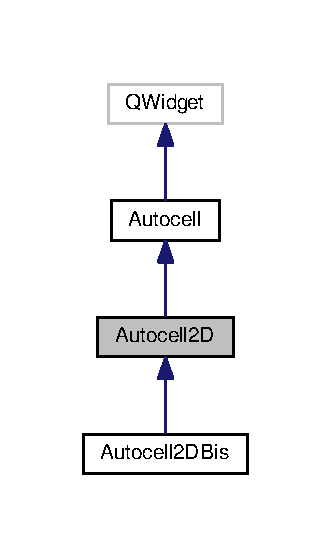
\includegraphics[width=159pt]{class_autocell2_d__inherit__graph}
\end{center}
\end{figure}


Graphe de collaboration de Autocell2D\+:\nopagebreak
\begin{figure}[H]
\begin{center}
\leavevmode
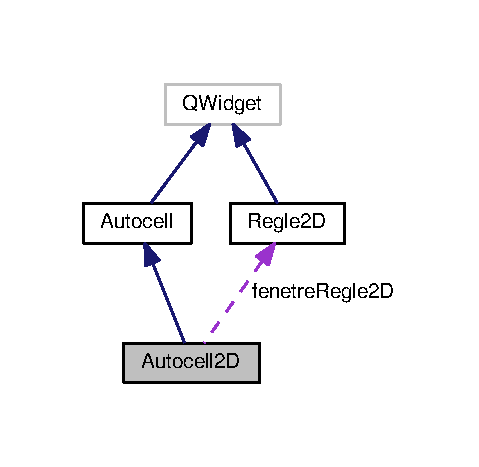
\includegraphics[width=230pt]{class_autocell2_d__coll__graph}
\end{center}
\end{figure}
\subsection*{Connecteurs publics}
\begin{DoxyCompactItemize}
\item 
void \hyperlink{class_autocell2_d_a08c17fc3e2ddf15173303d9e0d156e6e}{cell\+Selected} (int a, int b)
\begin{DoxyCompactList}\small\item\em S\+L\+OT qui modifie la. \end{DoxyCompactList}\item 
void \hyperlink{class_autocell2_d_ad698bee76cfdc81977864cd3db37ec2d}{clear} ()
\begin{DoxyCompactList}\small\item\em S\+L\+OT qui nettoie l\textquotesingle{}attribut membre etats. \end{DoxyCompactList}\item 
void \hyperlink{class_autocell2_d_aa5a7971b56710d08d3791a0c1b2a2c2e}{run\+Sim} ()
\begin{DoxyCompactList}\small\item\em S\+L\+OT qui simule un automate à 2 dimensions à l\textquotesingle{}aide des classes \hyperlink{class_automate2_d}{Automate2D} et \hyperlink{class_etat2_d}{Etat2D}. \end{DoxyCompactList}\item 
void \hyperlink{class_autocell2_d_acd5a8f9543affc825ddc82d840de7b42}{change\+Regle} (std\+::vector$<$ std\+::vector$<$ unsigned short int $>$ $>$ r, std\+::vector$<$ std\+::string $>$ c)
\begin{DoxyCompactList}\small\item\em S\+L\+OT change les attributs membres regle et couleur. \end{DoxyCompactList}\end{DoxyCompactItemize}
\subsection*{Fonctions membres publiques}
\begin{DoxyCompactItemize}
\item 
\hyperlink{class_autocell2_d_a2e7a6a59840288dc34fef654e45f7122}{Autocell2D} (Q\+Widget $\ast$parent=nullptr)
\begin{DoxyCompactList}\small\item\em Constructeur. \end{DoxyCompactList}\item 
virtual \hyperlink{class_autocell2_d_a0e48b49cea05335ce1fb24d078d5b2c4}{$\sim$\+Autocell2D} ()
\begin{DoxyCompactList}\small\item\em destructeur \end{DoxyCompactList}\item 
void \hyperlink{class_autocell2_d_a66bf641f01edbcb5c09fb1d3c97d45c5}{set\+Continu} (bool a)
\begin{DoxyCompactList}\small\item\em change le mode de lecture \end{DoxyCompactList}\item 
bool \hyperlink{class_autocell2_d_a96ed8e1716be3afb516e849d974d9eaf}{get\+Continu} ()
\begin{DoxyCompactList}\small\item\em retourne le mode de lecture \end{DoxyCompactList}\item 
virtual void \hyperlink{class_autocell2_d_a76ab804bc939ebe1957dd2ba3ea93803}{adjust\+Taille} ()
\begin{DoxyCompactList}\small\item\em ajuste la taille de la fenêtre en fonction de la largeur, la hauteur et la taille méthode virtuelle \end{DoxyCompactList}\item 
void \hyperlink{class_autocell2_d_abe5b8001ab6709eac849b03edac0c291}{set\+Regle} (std\+::vector$<$ std\+::vector$<$ unsigned short int $>$$>$ r)
\begin{DoxyCompactList}\small\item\em change la règle \end{DoxyCompactList}\item 
const std\+::vector$<$ std\+::vector$<$ unsigned short int $>$ $>$ \& \hyperlink{class_autocell2_d_a28140bde1d71db705c86ce1ace4cbea2}{get\+Regle} () const 
\begin{DoxyCompactList}\small\item\em retourne la règle \end{DoxyCompactList}\item 
virtual void \hyperlink{class_autocell2_d_a9380918c9f11ff223223672685b2cdb7}{init} ()
\begin{DoxyCompactList}\small\item\em initialise un état de départ pour l\textquotesingle{}attribut membre etats aléatoirement \end{DoxyCompactList}\item 
virtual void \hyperlink{class_autocell2_d_acd5f269beafa7f81ff57d6f05013892e}{init\+Sym} ()
\begin{DoxyCompactList}\small\item\em initialise un état de départ pour l\textquotesingle{}attribut membre etats symétriquement \end{DoxyCompactList}\item 
const Q\+Table\+Widget $\ast$ \hyperlink{class_autocell2_d_a1ee194d270b5ceff6085db31dbe9b3f4}{get\+\_\+etats} () const 
\begin{DoxyCompactList}\small\item\em retourne l\textquotesingle{}attribut membre etats \end{DoxyCompactList}\item 
\hyperlink{class_regle2_d}{Regle2D} $\ast$ \hyperlink{class_autocell2_d_a11c091d8075cdf351df8e567695f2093}{get\+\_\+regle2D} ()
\begin{DoxyCompactList}\small\item\em retourne l\textquotesingle{}attribut membre regle, permet les modifications \end{DoxyCompactList}\item 
const \hyperlink{class_regle2_d}{Regle2D} $\ast$ \hyperlink{class_autocell2_d_aaedf2f6ad98bfc023850ec0f1ce3e4bd}{get\+\_\+regle2D} () const 
\begin{DoxyCompactList}\small\item\em retourne l\textquotesingle{}attribut membre regle, ne permet pas la modification \end{DoxyCompactList}\item 
void \hyperlink{class_autocell2_d_ab7fbe02d26468c6f65f6510fb3f7862a}{set\+Etats} (unsigned int i, unsigned int j, Q\+String color)
\begin{DoxyCompactList}\small\item\em modifie la cellule (i,j) de la grille etats \end{DoxyCompactList}\end{DoxyCompactItemize}
\subsection*{Fonctions membres protégées}
\begin{DoxyCompactItemize}
\item 
void \hyperlink{class_autocell2_d_a470fdb5c648b9b0e951476fb9d5f3b96}{set\+Etat} (int h, int l)
\begin{DoxyCompactList}\small\item\em initialise l\textquotesingle{}attribut membre etats \end{DoxyCompactList}\end{DoxyCompactItemize}
\subsection*{Attributs protégés}
\begin{DoxyCompactItemize}
\item 
std\+::vector$<$ std\+::vector$<$ unsigned short int $>$ $>$ \hyperlink{class_autocell2_d_a238eef6674e510f6ce39d93427c6cad5}{regle}
\item 
Q\+Grid\+Layout $\ast$ \hyperlink{class_autocell2_d_ae935ff1610be1b1375f62b6877c35afb}{layout}
\item 
Q\+Table\+Widget $\ast$ \hyperlink{class_autocell2_d_a3a7359db79b875b93bcf89ab8377cf7e}{etats} = nullptr
\item 
\hyperlink{class_regle2_d}{Regle2D} $\ast$ \hyperlink{class_autocell2_d_a46226226228ceb3dd4c5cd4a04867a85}{fenetre\+Regle2D}
\item 
unsigned int \hyperlink{class_autocell2_d_a8d5918116d265492d58a7cdddd7de49d}{compteur} =0
\item 
Q\+Label $\ast$ \hyperlink{class_autocell2_d_a77c628582ad0c795ec3d2e1733f2d53f}{nb\+Simu}
\end{DoxyCompactItemize}
\subsection*{Membres hérités additionnels}


\subsection{Description détaillée}
Hérite de \hyperlink{class_autocell}{Autocell}. La classe \hyperlink{class_autocell2_d}{Autocell2D} permet de lancer des automates cellulaires à 2\+Dimensions (classe \hyperlink{class_automate2_d}{Automate2D} et \hyperlink{class_etat2_d}{Etat2D}) 

\subsection{Documentation des constructeurs et destructeur}
\index{Autocell2D@{Autocell2D}!Autocell2D@{Autocell2D}}
\index{Autocell2D@{Autocell2D}!Autocell2D@{Autocell2D}}
\subsubsection[{\texorpdfstring{Autocell2\+D(\+Q\+Widget $\ast$parent=nullptr)}{Autocell2D(QWidget *parent=nullptr)}}]{\setlength{\rightskip}{0pt plus 5cm}Autocell2\+D\+::\+Autocell2D (
\begin{DoxyParamCaption}
\item[{Q\+Widget $\ast$}]{parent = {\ttfamily nullptr}}
\end{DoxyParamCaption}
)}\hypertarget{class_autocell2_d_a2e7a6a59840288dc34fef654e45f7122}{}\label{class_autocell2_d_a2e7a6a59840288dc34fef654e45f7122}


Constructeur. 

\index{Autocell2D@{Autocell2D}!````~Autocell2D@{$\sim$\+Autocell2D}}
\index{````~Autocell2D@{$\sim$\+Autocell2D}!Autocell2D@{Autocell2D}}
\subsubsection[{\texorpdfstring{$\sim$\+Autocell2\+D()}{~Autocell2D()}}]{\setlength{\rightskip}{0pt plus 5cm}virtual Autocell2\+D\+::$\sim$\+Autocell2D (
\begin{DoxyParamCaption}
{}
\end{DoxyParamCaption}
)\hspace{0.3cm}{\ttfamily [inline]}, {\ttfamily [virtual]}}\hypertarget{class_autocell2_d_a0e48b49cea05335ce1fb24d078d5b2c4}{}\label{class_autocell2_d_a0e48b49cea05335ce1fb24d078d5b2c4}


destructeur 



\subsection{Documentation des fonctions membres}
\index{Autocell2D@{Autocell2D}!adjust\+Taille@{adjust\+Taille}}
\index{adjust\+Taille@{adjust\+Taille}!Autocell2D@{Autocell2D}}
\subsubsection[{\texorpdfstring{adjust\+Taille()}{adjustTaille()}}]{\setlength{\rightskip}{0pt plus 5cm}void Autocell2\+D\+::adjust\+Taille (
\begin{DoxyParamCaption}
{}
\end{DoxyParamCaption}
)\hspace{0.3cm}{\ttfamily [virtual]}}\hypertarget{class_autocell2_d_a76ab804bc939ebe1957dd2ba3ea93803}{}\label{class_autocell2_d_a76ab804bc939ebe1957dd2ba3ea93803}


ajuste la taille de la fenêtre en fonction de la largeur, la hauteur et la taille méthode virtuelle 



Implémente \hyperlink{class_autocell_a060d956fa55ae3871081b3ecb949689f}{Autocell}.

\index{Autocell2D@{Autocell2D}!cell\+Selected@{cell\+Selected}}
\index{cell\+Selected@{cell\+Selected}!Autocell2D@{Autocell2D}}
\subsubsection[{\texorpdfstring{cell\+Selected}{cellSelected}}]{\setlength{\rightskip}{0pt plus 5cm}void Autocell2\+D\+::cell\+Selected (
\begin{DoxyParamCaption}
\item[{int}]{a, }
\item[{int}]{b}
\end{DoxyParamCaption}
)\hspace{0.3cm}{\ttfamily [slot]}}\hypertarget{class_autocell2_d_a08c17fc3e2ddf15173303d9e0d156e6e}{}\label{class_autocell2_d_a08c17fc3e2ddf15173303d9e0d156e6e}


S\+L\+OT qui modifie la. 


\begin{DoxyParams}{Paramètres}
{\em a} & ligne\+: int \\
\hline
{\em b} & colonne\+: int \\
\hline
\end{DoxyParams}
\index{Autocell2D@{Autocell2D}!change\+Regle@{change\+Regle}}
\index{change\+Regle@{change\+Regle}!Autocell2D@{Autocell2D}}
\subsubsection[{\texorpdfstring{change\+Regle}{changeRegle}}]{\setlength{\rightskip}{0pt plus 5cm}void Autocell2\+D\+::change\+Regle (
\begin{DoxyParamCaption}
\item[{std\+::vector$<$ std\+::vector$<$ unsigned short int $>$ $>$}]{r, }
\item[{std\+::vector$<$ std\+::string $>$}]{c}
\end{DoxyParamCaption}
)\hspace{0.3cm}{\ttfamily [slot]}}\hypertarget{class_autocell2_d_acd5a8f9543affc825ddc82d840de7b42}{}\label{class_autocell2_d_acd5a8f9543affc825ddc82d840de7b42}


S\+L\+OT change les attributs membres regle et couleur. 


\begin{DoxyParams}{Paramètres}
{\em r} & \+:nouvelle règle\+: std\+::vector$<$std\+::vector$<$unsigned short int$>$ $>$ \\
\hline
{\em c} & \+:nouvelles couleurs\+: std\+::vector$<$std\+::string$>$ \\
\hline
\end{DoxyParams}
\index{Autocell2D@{Autocell2D}!clear@{clear}}
\index{clear@{clear}!Autocell2D@{Autocell2D}}
\subsubsection[{\texorpdfstring{clear}{clear}}]{\setlength{\rightskip}{0pt plus 5cm}void Autocell2\+D\+::clear (
\begin{DoxyParamCaption}
{}
\end{DoxyParamCaption}
)\hspace{0.3cm}{\ttfamily [slot]}}\hypertarget{class_autocell2_d_ad698bee76cfdc81977864cd3db37ec2d}{}\label{class_autocell2_d_ad698bee76cfdc81977864cd3db37ec2d}


S\+L\+OT qui nettoie l\textquotesingle{}attribut membre etats. 

\index{Autocell2D@{Autocell2D}!get\+\_\+etats@{get\+\_\+etats}}
\index{get\+\_\+etats@{get\+\_\+etats}!Autocell2D@{Autocell2D}}
\subsubsection[{\texorpdfstring{get\+\_\+etats() const }{get_etats() const }}]{\setlength{\rightskip}{0pt plus 5cm}const Q\+Table\+Widget$\ast$ Autocell2\+D\+::get\+\_\+etats (
\begin{DoxyParamCaption}
{}
\end{DoxyParamCaption}
) const\hspace{0.3cm}{\ttfamily [inline]}}\hypertarget{class_autocell2_d_a1ee194d270b5ceff6085db31dbe9b3f4}{}\label{class_autocell2_d_a1ee194d270b5ceff6085db31dbe9b3f4}


retourne l\textquotesingle{}attribut membre etats 

\begin{DoxyReturn}{Renvoie}
etats\+: const Q\+Table\+Widget$\ast$ 
\end{DoxyReturn}
\index{Autocell2D@{Autocell2D}!get\+\_\+regle2D@{get\+\_\+regle2D}}
\index{get\+\_\+regle2D@{get\+\_\+regle2D}!Autocell2D@{Autocell2D}}
\subsubsection[{\texorpdfstring{get\+\_\+regle2\+D()}{get_regle2D()}}]{\setlength{\rightskip}{0pt plus 5cm}{\bf Regle2D}$\ast$ Autocell2\+D\+::get\+\_\+regle2D (
\begin{DoxyParamCaption}
{}
\end{DoxyParamCaption}
)\hspace{0.3cm}{\ttfamily [inline]}}\hypertarget{class_autocell2_d_a11c091d8075cdf351df8e567695f2093}{}\label{class_autocell2_d_a11c091d8075cdf351df8e567695f2093}


retourne l\textquotesingle{}attribut membre regle, permet les modifications 

\begin{DoxyReturn}{Renvoie}
etats\+: Regle2\+D$\ast$ 
\end{DoxyReturn}
\index{Autocell2D@{Autocell2D}!get\+\_\+regle2D@{get\+\_\+regle2D}}
\index{get\+\_\+regle2D@{get\+\_\+regle2D}!Autocell2D@{Autocell2D}}
\subsubsection[{\texorpdfstring{get\+\_\+regle2\+D() const }{get_regle2D() const }}]{\setlength{\rightskip}{0pt plus 5cm}const {\bf Regle2D}$\ast$ Autocell2\+D\+::get\+\_\+regle2D (
\begin{DoxyParamCaption}
{}
\end{DoxyParamCaption}
) const\hspace{0.3cm}{\ttfamily [inline]}}\hypertarget{class_autocell2_d_aaedf2f6ad98bfc023850ec0f1ce3e4bd}{}\label{class_autocell2_d_aaedf2f6ad98bfc023850ec0f1ce3e4bd}


retourne l\textquotesingle{}attribut membre regle, ne permet pas la modification 

\begin{DoxyReturn}{Renvoie}
etats\+: const Regle2\+D$\ast$ 
\end{DoxyReturn}
\index{Autocell2D@{Autocell2D}!get\+Continu@{get\+Continu}}
\index{get\+Continu@{get\+Continu}!Autocell2D@{Autocell2D}}
\subsubsection[{\texorpdfstring{get\+Continu()}{getContinu()}}]{\setlength{\rightskip}{0pt plus 5cm}bool Autocell2\+D\+::get\+Continu (
\begin{DoxyParamCaption}
{}
\end{DoxyParamCaption}
)\hspace{0.3cm}{\ttfamily [inline]}}\hypertarget{class_autocell2_d_a96ed8e1716be3afb516e849d974d9eaf}{}\label{class_autocell2_d_a96ed8e1716be3afb516e849d974d9eaf}


retourne le mode de lecture 

\begin{DoxyReturn}{Renvoie}
mode de lecture\+: bool 
\end{DoxyReturn}
\index{Autocell2D@{Autocell2D}!get\+Regle@{get\+Regle}}
\index{get\+Regle@{get\+Regle}!Autocell2D@{Autocell2D}}
\subsubsection[{\texorpdfstring{get\+Regle() const }{getRegle() const }}]{\setlength{\rightskip}{0pt plus 5cm}const std\+::vector$<$std\+::vector$<$unsigned short int$>$ $>$\& Autocell2\+D\+::get\+Regle (
\begin{DoxyParamCaption}
{}
\end{DoxyParamCaption}
) const\hspace{0.3cm}{\ttfamily [inline]}}\hypertarget{class_autocell2_d_a28140bde1d71db705c86ce1ace4cbea2}{}\label{class_autocell2_d_a28140bde1d71db705c86ce1ace4cbea2}


retourne la règle 

\begin{DoxyReturn}{Renvoie}
règle\+: const std\+::vector$<$std\+::vector$<$unsigned short int$>$$>$\& 
\end{DoxyReturn}
\index{Autocell2D@{Autocell2D}!init@{init}}
\index{init@{init}!Autocell2D@{Autocell2D}}
\subsubsection[{\texorpdfstring{init()}{init()}}]{\setlength{\rightskip}{0pt plus 5cm}void Autocell2\+D\+::init (
\begin{DoxyParamCaption}
{}
\end{DoxyParamCaption}
)\hspace{0.3cm}{\ttfamily [virtual]}}\hypertarget{class_autocell2_d_a9380918c9f11ff223223672685b2cdb7}{}\label{class_autocell2_d_a9380918c9f11ff223223672685b2cdb7}


initialise un état de départ pour l\textquotesingle{}attribut membre etats aléatoirement 



Implémente \hyperlink{class_autocell_ac505c956de1d90a48e2d3558bdf97253}{Autocell}.

\index{Autocell2D@{Autocell2D}!init\+Sym@{init\+Sym}}
\index{init\+Sym@{init\+Sym}!Autocell2D@{Autocell2D}}
\subsubsection[{\texorpdfstring{init\+Sym()}{initSym()}}]{\setlength{\rightskip}{0pt plus 5cm}void Autocell2\+D\+::init\+Sym (
\begin{DoxyParamCaption}
{}
\end{DoxyParamCaption}
)\hspace{0.3cm}{\ttfamily [virtual]}}\hypertarget{class_autocell2_d_acd5f269beafa7f81ff57d6f05013892e}{}\label{class_autocell2_d_acd5f269beafa7f81ff57d6f05013892e}


initialise un état de départ pour l\textquotesingle{}attribut membre etats symétriquement 



Implémente \hyperlink{class_autocell_aa1e1870af0142596a9a81afe7f300a11}{Autocell}.

\index{Autocell2D@{Autocell2D}!run\+Sim@{run\+Sim}}
\index{run\+Sim@{run\+Sim}!Autocell2D@{Autocell2D}}
\subsubsection[{\texorpdfstring{run\+Sim}{runSim}}]{\setlength{\rightskip}{0pt plus 5cm}void Autocell2\+D\+::run\+Sim (
\begin{DoxyParamCaption}
{}
\end{DoxyParamCaption}
)\hspace{0.3cm}{\ttfamily [slot]}}\hypertarget{class_autocell2_d_aa5a7971b56710d08d3791a0c1b2a2c2e}{}\label{class_autocell2_d_aa5a7971b56710d08d3791a0c1b2a2c2e}


S\+L\+OT qui simule un automate à 2 dimensions à l\textquotesingle{}aide des classes \hyperlink{class_automate2_d}{Automate2D} et \hyperlink{class_etat2_d}{Etat2D}. 

\index{Autocell2D@{Autocell2D}!set\+Continu@{set\+Continu}}
\index{set\+Continu@{set\+Continu}!Autocell2D@{Autocell2D}}
\subsubsection[{\texorpdfstring{set\+Continu(bool a)}{setContinu(bool a)}}]{\setlength{\rightskip}{0pt plus 5cm}void Autocell2\+D\+::set\+Continu (
\begin{DoxyParamCaption}
\item[{bool}]{a}
\end{DoxyParamCaption}
)\hspace{0.3cm}{\ttfamily [inline]}}\hypertarget{class_autocell2_d_a66bf641f01edbcb5c09fb1d3c97d45c5}{}\label{class_autocell2_d_a66bf641f01edbcb5c09fb1d3c97d45c5}


change le mode de lecture 


\begin{DoxyParams}{Paramètres}
{\em mode} & de lecture\+: bool \\
\hline
\end{DoxyParams}
\index{Autocell2D@{Autocell2D}!set\+Etat@{set\+Etat}}
\index{set\+Etat@{set\+Etat}!Autocell2D@{Autocell2D}}
\subsubsection[{\texorpdfstring{set\+Etat(int h, int l)}{setEtat(int h, int l)}}]{\setlength{\rightskip}{0pt plus 5cm}void Autocell2\+D\+::set\+Etat (
\begin{DoxyParamCaption}
\item[{int}]{h, }
\item[{int}]{l}
\end{DoxyParamCaption}
)\hspace{0.3cm}{\ttfamily [protected]}}\hypertarget{class_autocell2_d_a470fdb5c648b9b0e951476fb9d5f3b96}{}\label{class_autocell2_d_a470fdb5c648b9b0e951476fb9d5f3b96}


initialise l\textquotesingle{}attribut membre etats 


\begin{DoxyParams}{Paramètres}
{\em h} & \+: hauteur\+: int \\
\hline
{\em l} & \+: largeur\+: int \\
\hline
\end{DoxyParams}
\index{Autocell2D@{Autocell2D}!set\+Etats@{set\+Etats}}
\index{set\+Etats@{set\+Etats}!Autocell2D@{Autocell2D}}
\subsubsection[{\texorpdfstring{set\+Etats(unsigned int i, unsigned int j, Q\+String color)}{setEtats(unsigned int i, unsigned int j, QString color)}}]{\setlength{\rightskip}{0pt plus 5cm}void Autocell2\+D\+::set\+Etats (
\begin{DoxyParamCaption}
\item[{unsigned int}]{i, }
\item[{unsigned int}]{j, }
\item[{Q\+String}]{color}
\end{DoxyParamCaption}
)\hspace{0.3cm}{\ttfamily [inline]}}\hypertarget{class_autocell2_d_ab7fbe02d26468c6f65f6510fb3f7862a}{}\label{class_autocell2_d_ab7fbe02d26468c6f65f6510fb3f7862a}


modifie la cellule (i,j) de la grille etats 


\begin{DoxyParams}{Paramètres}
{\em i} & \+: ligne\+: int \\
\hline
{\em j} & \+: colonne\+: int \\
\hline
{\em color} & \+: couleur de la cellule \+: Q\+String \\
\hline
\end{DoxyParams}
\index{Autocell2D@{Autocell2D}!set\+Regle@{set\+Regle}}
\index{set\+Regle@{set\+Regle}!Autocell2D@{Autocell2D}}
\subsubsection[{\texorpdfstring{set\+Regle(std\+::vector$<$ std\+::vector$<$ unsigned short int $>$$>$ r)}{setRegle(std::vector< std::vector< unsigned short int >> r)}}]{\setlength{\rightskip}{0pt plus 5cm}void Autocell2\+D\+::set\+Regle (
\begin{DoxyParamCaption}
\item[{std\+::vector$<$ std\+::vector$<$ unsigned short int $>$$>$}]{r}
\end{DoxyParamCaption}
)\hspace{0.3cm}{\ttfamily [inline]}}\hypertarget{class_autocell2_d_abe5b8001ab6709eac849b03edac0c291}{}\label{class_autocell2_d_abe5b8001ab6709eac849b03edac0c291}


change la règle 


\begin{DoxyParams}{Paramètres}
{\em r} & nouvelle règle\+: std\+::vector$<$std\+::vector$<$unsigned short int$>$$>$ \\
\hline
\end{DoxyParams}


\subsection{Documentation des données membres}
\index{Autocell2D@{Autocell2D}!compteur@{compteur}}
\index{compteur@{compteur}!Autocell2D@{Autocell2D}}
\subsubsection[{\texorpdfstring{compteur}{compteur}}]{\setlength{\rightskip}{0pt plus 5cm}unsigned int Autocell2\+D\+::compteur =0\hspace{0.3cm}{\ttfamily [protected]}}\hypertarget{class_autocell2_d_a8d5918116d265492d58a7cdddd7de49d}{}\label{class_autocell2_d_a8d5918116d265492d58a7cdddd7de49d}
compte de nombre de simulation \index{Autocell2D@{Autocell2D}!etats@{etats}}
\index{etats@{etats}!Autocell2D@{Autocell2D}}
\subsubsection[{\texorpdfstring{etats}{etats}}]{\setlength{\rightskip}{0pt plus 5cm}Q\+Table\+Widget$\ast$ Autocell2\+D\+::etats = nullptr\hspace{0.3cm}{\ttfamily [protected]}}\hypertarget{class_autocell2_d_a3a7359db79b875b93bcf89ab8377cf7e}{}\label{class_autocell2_d_a3a7359db79b875b93bcf89ab8377cf7e}
représente les cellules de l\textquotesingle{}automates \index{Autocell2D@{Autocell2D}!fenetre\+Regle2D@{fenetre\+Regle2D}}
\index{fenetre\+Regle2D@{fenetre\+Regle2D}!Autocell2D@{Autocell2D}}
\subsubsection[{\texorpdfstring{fenetre\+Regle2D}{fenetreRegle2D}}]{\setlength{\rightskip}{0pt plus 5cm}{\bf Regle2D}$\ast$ Autocell2\+D\+::fenetre\+Regle2D\hspace{0.3cm}{\ttfamily [protected]}}\hypertarget{class_autocell2_d_a46226226228ceb3dd4c5cd4a04867a85}{}\label{class_autocell2_d_a46226226228ceb3dd4c5cd4a04867a85}
I\+HM pour rentrer les règles \index{Autocell2D@{Autocell2D}!layout@{layout}}
\index{layout@{layout}!Autocell2D@{Autocell2D}}
\subsubsection[{\texorpdfstring{layout}{layout}}]{\setlength{\rightskip}{0pt plus 5cm}Q\+Grid\+Layout$\ast$ Autocell2\+D\+::layout\hspace{0.3cm}{\ttfamily [protected]}}\hypertarget{class_autocell2_d_ae935ff1610be1b1375f62b6877c35afb}{}\label{class_autocell2_d_ae935ff1610be1b1375f62b6877c35afb}
layout principal \index{Autocell2D@{Autocell2D}!nb\+Simu@{nb\+Simu}}
\index{nb\+Simu@{nb\+Simu}!Autocell2D@{Autocell2D}}
\subsubsection[{\texorpdfstring{nb\+Simu}{nbSimu}}]{\setlength{\rightskip}{0pt plus 5cm}Q\+Label$\ast$ Autocell2\+D\+::nb\+Simu\hspace{0.3cm}{\ttfamily [protected]}}\hypertarget{class_autocell2_d_a77c628582ad0c795ec3d2e1733f2d53f}{}\label{class_autocell2_d_a77c628582ad0c795ec3d2e1733f2d53f}
compteur afficher sur l\textquotesingle{}autocell \index{Autocell2D@{Autocell2D}!regle@{regle}}
\index{regle@{regle}!Autocell2D@{Autocell2D}}
\subsubsection[{\texorpdfstring{regle}{regle}}]{\setlength{\rightskip}{0pt plus 5cm}std\+::vector$<$std\+::vector$<$unsigned short int$>$ $>$ Autocell2\+D\+::regle\hspace{0.3cm}{\ttfamily [protected]}}\hypertarget{class_autocell2_d_a238eef6674e510f6ce39d93427c6cad5}{}\label{class_autocell2_d_a238eef6674e510f6ce39d93427c6cad5}
enregistre la règle qui sera donnée à l\textquotesingle{}automate2D 

La documentation de cette classe a été générée à partir des fichiers suivants \+:\begin{DoxyCompactItemize}
\item 
/home/thomaspaita/\+Bureau/info/\+L\+O21/\+L\+O21/\+Auto\+Cell/\hyperlink{autocell_8h}{autocell.\+h}\item 
/home/thomaspaita/\+Bureau/info/\+L\+O21/\+L\+O21/\+Auto\+Cell/\hyperlink{autocell_8cpp}{autocell.\+cpp}\end{DoxyCompactItemize}

\hypertarget{class_autocell2_d_bis}{}\section{Référence de la classe Autocell2\+D\+Bis}
\label{class_autocell2_d_bis}\index{Autocell2\+D\+Bis@{Autocell2\+D\+Bis}}


Hérite de \hyperlink{class_autocell2_d}{Autocell2D}. La classe \hyperlink{class_autocell2_d_bis}{Autocell2\+D\+Bis} montre comment intégrer de nouvelles règles à un autocell2D.  




{\ttfamily \#include $<$autocell.\+h$>$}



Graphe d\textquotesingle{}héritage de Autocell2\+D\+Bis\+:
\nopagebreak
\begin{figure}[H]
\begin{center}
\leavevmode
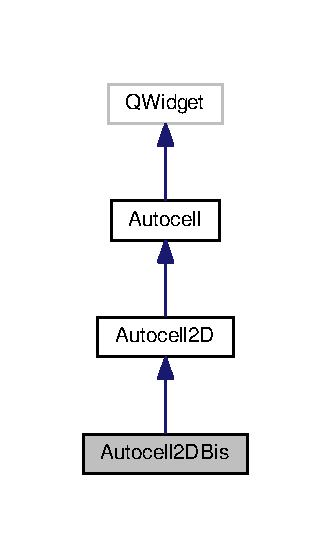
\includegraphics[width=159pt]{class_autocell2_d_bis__inherit__graph}
\end{center}
\end{figure}


Graphe de collaboration de Autocell2\+D\+Bis\+:
\nopagebreak
\begin{figure}[H]
\begin{center}
\leavevmode
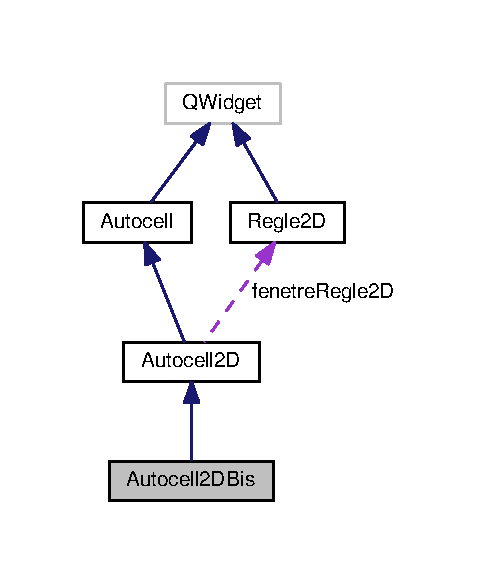
\includegraphics[width=230pt]{class_autocell2_d_bis__coll__graph}
\end{center}
\end{figure}
\subsection*{Fonctions membres publiques}
\begin{DoxyCompactItemize}
\item 
\hyperlink{class_autocell2_d_bis_ad6e848447a16085a06100c9375eb7819}{Autocell2\+D\+Bis} (Q\+Widget $\ast$parent=nullptr)
\begin{DoxyCompactList}\small\item\em Constructeur modification de la fenetre\+Regle2D et la remplaçant par un \hyperlink{class_regle2_d_bis}{Regle2\+D\+Bis}. \end{DoxyCompactList}\end{DoxyCompactItemize}
\subsection*{Membres hérités additionnels}


\subsection{Description détaillée}
Hérite de \hyperlink{class_autocell2_d}{Autocell2D}. La classe \hyperlink{class_autocell2_d_bis}{Autocell2\+D\+Bis} montre comment intégrer de nouvelles règles à un autocell2D. 

\subsection{Documentation des constructeurs et destructeur}
\index{Autocell2\+D\+Bis@{Autocell2\+D\+Bis}!Autocell2\+D\+Bis@{Autocell2\+D\+Bis}}
\index{Autocell2\+D\+Bis@{Autocell2\+D\+Bis}!Autocell2\+D\+Bis@{Autocell2\+D\+Bis}}
\subsubsection[{\texorpdfstring{Autocell2\+D\+Bis(\+Q\+Widget $\ast$parent=nullptr)}{Autocell2DBis(QWidget *parent=nullptr)}}]{\setlength{\rightskip}{0pt plus 5cm}Autocell2\+D\+Bis\+::\+Autocell2\+D\+Bis (
\begin{DoxyParamCaption}
\item[{Q\+Widget $\ast$}]{parent = {\ttfamily nullptr}}
\end{DoxyParamCaption}
)\hspace{0.3cm}{\ttfamily [inline]}}\hypertarget{class_autocell2_d_bis_ad6e848447a16085a06100c9375eb7819}{}\label{class_autocell2_d_bis_ad6e848447a16085a06100c9375eb7819}


Constructeur modification de la fenetre\+Regle2D et la remplaçant par un \hyperlink{class_regle2_d_bis}{Regle2\+D\+Bis}. 



La documentation de cette classe a été générée à partir du fichier suivant \+:\begin{DoxyCompactItemize}
\item 
info/\+L\+O21/\+L\+O21/\+Auto\+Cell/\hyperlink{autocell_8h}{autocell.\+h}\end{DoxyCompactItemize}

\hypertarget{class_automate}{}\section{Référence du modèle de la classe Automate$<$ T $>$}
\label{class_automate}\index{Automate$<$ T $>$@{Automate$<$ T $>$}}


Classe Template abstraite.  




{\ttfamily \#include $<$Automate.\+h$>$}

\subsection*{Fonctions membres publiques}
\begin{DoxyCompactItemize}
\item 
\hyperlink{class_automate_a3215065f896b7297a676219a0d80a045}{Automate} (unsigned short int nb\+Etat=2)
\begin{DoxyCompactList}\small\item\em Constructeur. \end{DoxyCompactList}\item 
void \hyperlink{class_automate_afcf89728c989465400a19174ef22dfa5}{set\+Nb\+Etat} (unsigned short int e)
\begin{DoxyCompactList}\small\item\em change le nombre d\textquotesingle{}état \end{DoxyCompactList}\item 
unsigned short int \hyperlink{class_automate_a80d9f6cfc6786ac21b51c4ab7fcb072d}{get\+Nb\+Etat} () const 
\begin{DoxyCompactList}\small\item\em retourne le nombre d\textquotesingle{}état \end{DoxyCompactList}\item 
virtual void \hyperlink{class_automate_abfeaddcc8930b1f63a785cd5c6ff6dc5}{appliquer\+Transition} (const T \&, T \&) const =0
\begin{DoxyCompactList}\small\item\em applique la transition entre deux quelconques donnés en paramètre Méthode virtuelle pure \end{DoxyCompactList}\end{DoxyCompactItemize}
\subsection*{Attributs privés}
\begin{DoxyCompactItemize}
\item 
unsigned short int \hyperlink{class_automate_aa3d97a653a0c0f20175237c03345d085}{m\+\_\+nb\+Etat}
\end{DoxyCompactItemize}


\subsection{Description détaillée}
\subsubsection*{template$<$class T$>$\\*
class Automate$<$ T $>$}

Classe Template abstraite. 

La classe généralise un \hyperlink{class_automate}{Automate} et définie la méthodes virtuelle qui devra être présente et définie dans chaque \hyperlink{class_automate}{Automate}. (run\+Sim()) 

\subsection{Documentation des constructeurs et destructeur}
\index{Automate@{Automate}!Automate@{Automate}}
\index{Automate@{Automate}!Automate@{Automate}}
\subsubsection[{\texorpdfstring{Automate(unsigned short int nb\+Etat=2)}{Automate(unsigned short int nbEtat=2)}}]{\setlength{\rightskip}{0pt plus 5cm}template$<$class T$>$ {\bf Automate}$<$ T $>$\+::{\bf Automate} (
\begin{DoxyParamCaption}
\item[{unsigned short int}]{nb\+Etat = {\ttfamily 2}}
\end{DoxyParamCaption}
)\hspace{0.3cm}{\ttfamily [inline]}}\hypertarget{class_automate_a3215065f896b7297a676219a0d80a045}{}\label{class_automate_a3215065f896b7297a676219a0d80a045}


Constructeur. 


\begin{DoxyParams}{Paramètres}
{\em nb\+Etat} & nombre d\textquotesingle{}états que peut prendre chaque cellule (2 par défaut)\+: unsigned short int \\
\hline
\end{DoxyParams}


\subsection{Documentation des fonctions membres}
\index{Automate@{Automate}!appliquer\+Transition@{appliquer\+Transition}}
\index{appliquer\+Transition@{appliquer\+Transition}!Automate@{Automate}}
\subsubsection[{\texorpdfstring{appliquer\+Transition(const T \&, T \&) const =0}{appliquerTransition(const T &, T &) const =0}}]{\setlength{\rightskip}{0pt plus 5cm}template$<$class T$>$ virtual void {\bf Automate}$<$ T $>$\+::appliquer\+Transition (
\begin{DoxyParamCaption}
\item[{const T \&}]{, }
\item[{T \&}]{}
\end{DoxyParamCaption}
) const\hspace{0.3cm}{\ttfamily [pure virtual]}}\hypertarget{class_automate_abfeaddcc8930b1f63a785cd5c6ff6dc5}{}\label{class_automate_abfeaddcc8930b1f63a785cd5c6ff6dc5}


applique la transition entre deux quelconques donnés en paramètre Méthode virtuelle pure 


\begin{DoxyParams}{Paramètres}
{\em depart} & \+: const T\& \\
\hline
{\em destination} & \+: T\& \\
\hline
\end{DoxyParams}


Implémenté dans \hyperlink{class_automate1_d_a46c4e3b65e6d657c93e54fcbbc022dc6}{Automate1D}, et \hyperlink{class_automate2_d_a2cbea145a6e7eff58528bcab31316365}{Automate2D}.

\index{Automate@{Automate}!get\+Nb\+Etat@{get\+Nb\+Etat}}
\index{get\+Nb\+Etat@{get\+Nb\+Etat}!Automate@{Automate}}
\subsubsection[{\texorpdfstring{get\+Nb\+Etat() const }{getNbEtat() const }}]{\setlength{\rightskip}{0pt plus 5cm}template$<$class T$>$ unsigned short int {\bf Automate}$<$ T $>$\+::get\+Nb\+Etat (
\begin{DoxyParamCaption}
{}
\end{DoxyParamCaption}
) const\hspace{0.3cm}{\ttfamily [inline]}}\hypertarget{class_automate_a80d9f6cfc6786ac21b51c4ab7fcb072d}{}\label{class_automate_a80d9f6cfc6786ac21b51c4ab7fcb072d}


retourne le nombre d\textquotesingle{}état 

\begin{DoxyReturn}{Renvoie}
m\+\_\+nb\+Etat \+: unsigned short int 
\end{DoxyReturn}
\index{Automate@{Automate}!set\+Nb\+Etat@{set\+Nb\+Etat}}
\index{set\+Nb\+Etat@{set\+Nb\+Etat}!Automate@{Automate}}
\subsubsection[{\texorpdfstring{set\+Nb\+Etat(unsigned short int e)}{setNbEtat(unsigned short int e)}}]{\setlength{\rightskip}{0pt plus 5cm}template$<$class T$>$ void {\bf Automate}$<$ T $>$\+::set\+Nb\+Etat (
\begin{DoxyParamCaption}
\item[{unsigned short int}]{e}
\end{DoxyParamCaption}
)\hspace{0.3cm}{\ttfamily [inline]}}\hypertarget{class_automate_afcf89728c989465400a19174ef22dfa5}{}\label{class_automate_afcf89728c989465400a19174ef22dfa5}


change le nombre d\textquotesingle{}état 


\begin{DoxyParams}{Paramètres}
{\em e} & \+: nouveau nombre d\textquotesingle{}état \+:unsigned short int \\
\hline
\end{DoxyParams}


\subsection{Documentation des données membres}
\index{Automate@{Automate}!m\+\_\+nb\+Etat@{m\+\_\+nb\+Etat}}
\index{m\+\_\+nb\+Etat@{m\+\_\+nb\+Etat}!Automate@{Automate}}
\subsubsection[{\texorpdfstring{m\+\_\+nb\+Etat}{m_nbEtat}}]{\setlength{\rightskip}{0pt plus 5cm}template$<$class T$>$ unsigned short int {\bf Automate}$<$ T $>$\+::m\+\_\+nb\+Etat\hspace{0.3cm}{\ttfamily [private]}}\hypertarget{class_automate_aa3d97a653a0c0f20175237c03345d085}{}\label{class_automate_aa3d97a653a0c0f20175237c03345d085}
Nombre d\textquotesingle{}état 

La documentation de cette classe a été générée à partir du fichier suivant \+:\begin{DoxyCompactItemize}
\item 
info/\+L\+O21/\+L\+O21/\+Auto\+Cell/\hyperlink{_automate_8h}{Automate.\+h}\end{DoxyCompactItemize}

\hypertarget{class_automate1_d}{}\section{Référence de la classe Automate1D}
\label{class_automate1_d}\index{Automate1D@{Automate1D}}


hérite de \hyperlink{class_automate}{Automate$<$\+Etat1\+D$>$}. La classe permet d\textquotesingle{}appliquer une transition sur les \hyperlink{class_etat1_d}{Etat1D} suivant une règle  




{\ttfamily \#include $<$Automate1\+D.\+h$>$}



Graphe d\textquotesingle{}héritage de Automate1D\+:\nopagebreak
\begin{figure}[H]
\begin{center}
\leavevmode
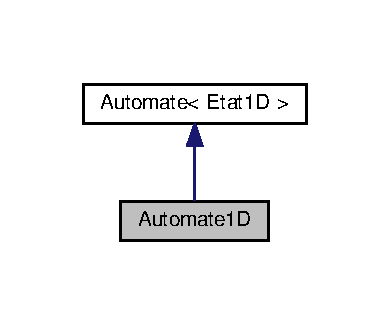
\includegraphics[width=187pt]{class_automate1_d__inherit__graph}
\end{center}
\end{figure}


Graphe de collaboration de Automate1D\+:\nopagebreak
\begin{figure}[H]
\begin{center}
\leavevmode
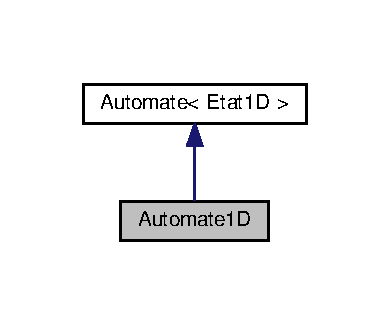
\includegraphics[width=187pt]{class_automate1_d__coll__graph}
\end{center}
\end{figure}
\subsection*{Fonctions membres publiques}
\begin{DoxyCompactItemize}
\item 
int \hyperlink{class_automate1_d_a3ad4c7b525674ea7abdfdaa5dbf3e83e}{get\+Numero} () const 
\begin{DoxyCompactList}\small\item\em accesseur en lecture \end{DoxyCompactList}\item 
std\+::string \hyperlink{class_automate1_d_a165ec2dbac45a6d8731fb564efb72095}{get\+Numero\+Bit} () const 
\begin{DoxyCompactList}\small\item\em accesseur en lecture \end{DoxyCompactList}\item 
void \hyperlink{class_automate1_d_a46c4e3b65e6d657c93e54fcbbc022dc6}{appliquer\+Transition} (const \hyperlink{class_etat1_d}{Etat1D} \&dep, \hyperlink{class_etat1_d}{Etat1D} \&dest) const 
\begin{DoxyCompactList}\small\item\em applique les règles de transition à un état \end{DoxyCompactList}\item 
void \hyperlink{class_automate1_d_ade2e9e03aef92b66c7f41f38e54e61b1}{afficher} () const 
\begin{DoxyCompactList}\small\item\em afficher un automate \end{DoxyCompactList}\end{DoxyCompactItemize}
\subsection*{Fonctions membres privées}
\begin{DoxyCompactItemize}
\item 
\hyperlink{class_automate1_d_a80210daacd80e5b0ce9132ac3c6d074c}{Automate1D} (short unsigned int num, unsigned short int nb\+Etat=2)
\begin{DoxyCompactList}\small\item\em Constructeur Privée. \end{DoxyCompactList}\item 
\hyperlink{class_automate1_d_a91c67e3e10240866e641c0824531acdb}{Automate1D} (const std\+::string \&num\+Bit, unsigned short int nb\+Etat=2)
\begin{DoxyCompactList}\small\item\em Constructeur Privée. \end{DoxyCompactList}\end{DoxyCompactItemize}
\subsection*{Attributs privés}
\begin{DoxyCompactItemize}
\item 
short unsigned int \hyperlink{class_automate1_d_a5ae877f5860e58fc17f6654b96b3aff8}{m\+\_\+numero}
\item 
std\+::string \hyperlink{class_automate1_d_a2a7ec50a64371b8b5dacd49844b712e3}{m\+\_\+numero\+Bit}
\end{DoxyCompactItemize}
\subsection*{Amis}
\begin{DoxyCompactItemize}
\item 
class \hyperlink{class_automate1_d_a6f30ee58a7bdd1cf1c712265d22f2faa}{Automate\+Manager}
\end{DoxyCompactItemize}


\subsection{Description détaillée}
hérite de \hyperlink{class_automate}{Automate$<$\+Etat1\+D$>$}. La classe permet d\textquotesingle{}appliquer une transition sur les \hyperlink{class_etat1_d}{Etat1D} suivant une règle 

\subsection{Documentation des constructeurs et destructeur}
\index{Automate1D@{Automate1D}!Automate1D@{Automate1D}}
\index{Automate1D@{Automate1D}!Automate1D@{Automate1D}}
\subsubsection[{\texorpdfstring{Automate1\+D(short unsigned int num, unsigned short int nb\+Etat=2)}{Automate1D(short unsigned int num, unsigned short int nbEtat=2)}}]{\setlength{\rightskip}{0pt plus 5cm}Automate1\+D\+::\+Automate1D (
\begin{DoxyParamCaption}
\item[{short unsigned int}]{num, }
\item[{unsigned short int}]{nb\+Etat = {\ttfamily 2}}
\end{DoxyParamCaption}
)\hspace{0.3cm}{\ttfamily [private]}}\hypertarget{class_automate1_d_a80210daacd80e5b0ce9132ac3c6d074c}{}\label{class_automate1_d_a80210daacd80e5b0ce9132ac3c6d074c}


Constructeur Privée. 


\begin{DoxyParams}{Paramètres}
{\em num} & \+: numéro de la régle\+: unsigned short int \\
\hline
{\em nb\+Etat} & \+: nombre d\textquotesingle{}état \+: unsigned short int \\
\hline
\end{DoxyParams}
\index{Automate1D@{Automate1D}!Automate1D@{Automate1D}}
\index{Automate1D@{Automate1D}!Automate1D@{Automate1D}}
\subsubsection[{\texorpdfstring{Automate1\+D(const std\+::string \&num\+Bit, unsigned short int nb\+Etat=2)}{Automate1D(const std::string &numBit, unsigned short int nbEtat=2)}}]{\setlength{\rightskip}{0pt plus 5cm}Automate1\+D\+::\+Automate1D (
\begin{DoxyParamCaption}
\item[{const std\+::string \&}]{num\+Bit, }
\item[{unsigned short int}]{nb\+Etat = {\ttfamily 2}}
\end{DoxyParamCaption}
)\hspace{0.3cm}{\ttfamily [private]}}\hypertarget{class_automate1_d_a91c67e3e10240866e641c0824531acdb}{}\label{class_automate1_d_a91c67e3e10240866e641c0824531acdb}


Constructeur Privée. 


\begin{DoxyParams}{Paramètres}
{\em num\+Bit} & \+: numéro de la régle\+: const std\+::string\& \\
\hline
{\em nb\+Etat} & \+: nombre d\textquotesingle{}état \+: unsigned short int \\
\hline
\end{DoxyParams}


\subsection{Documentation des fonctions membres}
\index{Automate1D@{Automate1D}!afficher@{afficher}}
\index{afficher@{afficher}!Automate1D@{Automate1D}}
\subsubsection[{\texorpdfstring{afficher() const }{afficher() const }}]{\setlength{\rightskip}{0pt plus 5cm}void Automate1\+D\+::afficher (
\begin{DoxyParamCaption}
{}
\end{DoxyParamCaption}
) const}\hypertarget{class_automate1_d_ade2e9e03aef92b66c7f41f38e54e61b1}{}\label{class_automate1_d_ade2e9e03aef92b66c7f41f38e54e61b1}


afficher un automate 

\index{Automate1D@{Automate1D}!appliquer\+Transition@{appliquer\+Transition}}
\index{appliquer\+Transition@{appliquer\+Transition}!Automate1D@{Automate1D}}
\subsubsection[{\texorpdfstring{appliquer\+Transition(const Etat1\+D \&dep, Etat1\+D \&dest) const }{appliquerTransition(const Etat1D &dep, Etat1D &dest) const }}]{\setlength{\rightskip}{0pt plus 5cm}void Automate1\+D\+::appliquer\+Transition (
\begin{DoxyParamCaption}
\item[{const {\bf Etat1D} \&}]{dep, }
\item[{{\bf Etat1D} \&}]{dest}
\end{DoxyParamCaption}
) const\hspace{0.3cm}{\ttfamily [virtual]}}\hypertarget{class_automate1_d_a46c4e3b65e6d657c93e54fcbbc022dc6}{}\label{class_automate1_d_a46c4e3b65e6d657c93e54fcbbc022dc6}


applique les règles de transition à un état 


\begin{DoxyParams}{Paramètres}
{\em dep} & \+: état de départ\+: const \hyperlink{class_etat1_d}{Etat1D}\& \\
\hline
{\em dest} & \+: etat d\textquotesingle{}arrivé\+: \hyperlink{class_etat1_d}{Etat1D}\& \\
\hline
\end{DoxyParams}


Implémente \hyperlink{class_automate_abfeaddcc8930b1f63a785cd5c6ff6dc5}{Automate$<$ Etat1\+D $>$}.

\index{Automate1D@{Automate1D}!get\+Numero@{get\+Numero}}
\index{get\+Numero@{get\+Numero}!Automate1D@{Automate1D}}
\subsubsection[{\texorpdfstring{get\+Numero() const }{getNumero() const }}]{\setlength{\rightskip}{0pt plus 5cm}int Automate1\+D\+::get\+Numero (
\begin{DoxyParamCaption}
{}
\end{DoxyParamCaption}
) const}\hypertarget{class_automate1_d_a3ad4c7b525674ea7abdfdaa5dbf3e83e}{}\label{class_automate1_d_a3ad4c7b525674ea7abdfdaa5dbf3e83e}


accesseur en lecture 

\begin{DoxyReturn}{Renvoie}
m\+\_\+numero \+: numéro de la règle\+: int 
\end{DoxyReturn}
\index{Automate1D@{Automate1D}!get\+Numero\+Bit@{get\+Numero\+Bit}}
\index{get\+Numero\+Bit@{get\+Numero\+Bit}!Automate1D@{Automate1D}}
\subsubsection[{\texorpdfstring{get\+Numero\+Bit() const }{getNumeroBit() const }}]{\setlength{\rightskip}{0pt plus 5cm}std\+::string Automate1\+D\+::get\+Numero\+Bit (
\begin{DoxyParamCaption}
{}
\end{DoxyParamCaption}
) const}\hypertarget{class_automate1_d_a165ec2dbac45a6d8731fb564efb72095}{}\label{class_automate1_d_a165ec2dbac45a6d8731fb564efb72095}


accesseur en lecture 

\begin{DoxyReturn}{Renvoie}
m\+\_\+numero\+Bit \+: numéro de la règle\+: std\+::string 
\end{DoxyReturn}


\subsection{Documentation des fonctions amies et associées}
\index{Automate1D@{Automate1D}!Automate\+Manager@{Automate\+Manager}}
\index{Automate\+Manager@{Automate\+Manager}!Automate1D@{Automate1D}}
\subsubsection[{\texorpdfstring{Automate\+Manager}{AutomateManager}}]{\setlength{\rightskip}{0pt plus 5cm}friend class {\bf Automate\+Manager}\hspace{0.3cm}{\ttfamily [friend]}}\hypertarget{class_automate1_d_a6f30ee58a7bdd1cf1c712265d22f2faa}{}\label{class_automate1_d_a6f30ee58a7bdd1cf1c712265d22f2faa}


\subsection{Documentation des données membres}
\index{Automate1D@{Automate1D}!m\+\_\+numero@{m\+\_\+numero}}
\index{m\+\_\+numero@{m\+\_\+numero}!Automate1D@{Automate1D}}
\subsubsection[{\texorpdfstring{m\+\_\+numero}{m_numero}}]{\setlength{\rightskip}{0pt plus 5cm}short unsigned int Automate1\+D\+::m\+\_\+numero\hspace{0.3cm}{\ttfamily [private]}}\hypertarget{class_automate1_d_a5ae877f5860e58fc17f6654b96b3aff8}{}\label{class_automate1_d_a5ae877f5860e58fc17f6654b96b3aff8}
Numéro de la règle \index{Automate1D@{Automate1D}!m\+\_\+numero\+Bit@{m\+\_\+numero\+Bit}}
\index{m\+\_\+numero\+Bit@{m\+\_\+numero\+Bit}!Automate1D@{Automate1D}}
\subsubsection[{\texorpdfstring{m\+\_\+numero\+Bit}{m_numeroBit}}]{\setlength{\rightskip}{0pt plus 5cm}std\+::string Automate1\+D\+::m\+\_\+numero\+Bit\hspace{0.3cm}{\ttfamily [private]}}\hypertarget{class_automate1_d_a2a7ec50a64371b8b5dacd49844b712e3}{}\label{class_automate1_d_a2a7ec50a64371b8b5dacd49844b712e3}
Numéro de la règle sous un autre format 

La documentation de cette classe a été générée à partir des fichiers suivants \+:\begin{DoxyCompactItemize}
\item 
info/\+L\+O21/\+L\+O21/\+Auto\+Cell/\hyperlink{_automate1_d_8h}{Automate1\+D.\+h}\item 
info/\+L\+O21/\+L\+O21/\+Auto\+Cell/\hyperlink{_automate1_d_8cpp}{Automate1\+D.\+cpp}\end{DoxyCompactItemize}

\hypertarget{class_automate2_d}{}\section{Référence de la classe Automate2D}
\label{class_automate2_d}\index{Automate2D@{Automate2D}}


hérite de \hyperlink{class_automate}{Automate$<$\+Etat2\+D$>$}. La classe permet d\textquotesingle{}appliquer une transition sur les \hyperlink{class_etat2_d}{Etat2D} en suivant des règles  




{\ttfamily \#include $<$Automate2\+D.\+h$>$}



Graphe d\textquotesingle{}héritage de Automate2D\+:\nopagebreak
\begin{figure}[H]
\begin{center}
\leavevmode
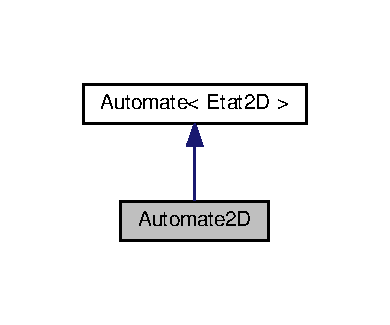
\includegraphics[width=187pt]{class_automate2_d__inherit__graph}
\end{center}
\end{figure}


Graphe de collaboration de Automate2D\+:\nopagebreak
\begin{figure}[H]
\begin{center}
\leavevmode
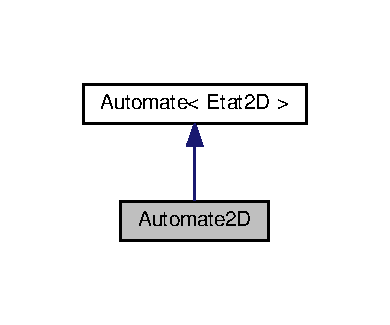
\includegraphics[width=187pt]{class_automate2_d__coll__graph}
\end{center}
\end{figure}
\subsection*{Fonctions membres publiques}
\begin{DoxyCompactItemize}
\item 
virtual \hyperlink{class_automate2_d_a20624efccdb4ec55afe6259f51ce3dd2}{$\sim$\+Automate2D} ()
\begin{DoxyCompactList}\small\item\em Destructeur virtuel. \end{DoxyCompactList}\item 
std\+::vector$<$ std\+::vector$<$ unsigned short int $>$ $>$ \hyperlink{class_automate2_d_a0140faf046124a3d6c1792ca8493f60b}{get\+Regle} () const 
\begin{DoxyCompactList}\small\item\em accesseur lecture \end{DoxyCompactList}\item 
void \hyperlink{class_automate2_d_a250f624adbe858ecbb17784730845248}{set\+Regle} (std\+::vector$<$ std\+::vector$<$ unsigned short int $>$ $>$ const \&new\+Regle)
\begin{DoxyCompactList}\small\item\em modifie la règle \end{DoxyCompactList}\item 
virtual bool \hyperlink{class_automate2_d_a2cc86edfb8c2ec56a645247449b94c16}{appliquer\+Transition} (const \hyperlink{class_etat2_d}{Etat2D} \&dep, \hyperlink{class_etat2_d}{Etat2D} \&dest) const 
\begin{DoxyCompactList}\small\item\em applique la transition entre 2 Etats en fonction de la règle \end{DoxyCompactList}\item 
int \hyperlink{class_automate2_d_a067188a9e1b3afc554fc195e20cd60e8}{nb\+Cellule} (unsigned int i, unsigned int j, \hyperlink{class_etat2_d}{Etat2D} const \&etat, unsigned short int etat\+Cel) const 
\begin{DoxyCompactList}\small\item\em compte le nombre de cellules alentours dans l\textquotesingle{}état etat\+Cel \end{DoxyCompactList}\end{DoxyCompactItemize}
\subsection*{Fonctions membres protégées}
\begin{DoxyCompactItemize}
\item 
\hyperlink{class_automate2_d_ae00c4fae1c73cbac83424d576cfbd23d}{Automate2D} (std\+::vector$<$ std\+::vector$<$ unsigned short int $>$ $>$ regle=std\+::vector$<$ std\+::vector$<$ unsigned short int $>$ $>$(), unsigned short int nb\+Etat=2)
\begin{DoxyCompactList}\small\item\em Constructeur Protected. \end{DoxyCompactList}\end{DoxyCompactItemize}
\subsection*{Attributs protégés}
\begin{DoxyCompactItemize}
\item 
std\+::vector$<$ std\+::vector$<$ unsigned short int $>$ $>$ \hyperlink{class_automate2_d_ac894413963ffddd67dc899e64a41bca0}{m\+\_\+regle}
\end{DoxyCompactItemize}
\subsection*{Amis}
\begin{DoxyCompactItemize}
\item 
class \hyperlink{class_automate2_d_ae4af0b43eae2d17cf68916ad9e636cd8}{Automate\+Manager2D}
\end{DoxyCompactItemize}


\subsection{Description détaillée}
hérite de \hyperlink{class_automate}{Automate$<$\+Etat2\+D$>$}. La classe permet d\textquotesingle{}appliquer une transition sur les \hyperlink{class_etat2_d}{Etat2D} en suivant des règles 

\subsection{Documentation des constructeurs et destructeur}
\index{Automate2D@{Automate2D}!Automate2D@{Automate2D}}
\index{Automate2D@{Automate2D}!Automate2D@{Automate2D}}
\subsubsection[{\texorpdfstring{Automate2\+D(std\+::vector$<$ std\+::vector$<$ unsigned short int $>$ $>$ regle=std\+::vector$<$ std\+::vector$<$ unsigned short int $>$ $>$(), unsigned short int nb\+Etat=2)}{Automate2D(std::vector< std::vector< unsigned short int > > regle=std::vector< std::vector< unsigned short int > >(), unsigned short int nbEtat=2)}}]{\setlength{\rightskip}{0pt plus 5cm}Automate2\+D\+::\+Automate2D (
\begin{DoxyParamCaption}
\item[{std\+::vector$<$ std\+::vector$<$ unsigned short int $>$ $>$}]{regle = {\ttfamily std\+:\+:vector$<$~std\+:\+:vector$<$unsigned~short~int$>$~$>$()}, }
\item[{unsigned short int}]{nb\+Etat = {\ttfamily 2}}
\end{DoxyParamCaption}
)\hspace{0.3cm}{\ttfamily [inline]}, {\ttfamily [protected]}}\hypertarget{class_automate2_d_ae00c4fae1c73cbac83424d576cfbd23d}{}\label{class_automate2_d_ae00c4fae1c73cbac83424d576cfbd23d}


Constructeur Protected. 


\begin{DoxyParams}{Paramètres}
{\em regle} & \+: std\+::vector$<$ std\+::vector$<$unsigned short int$>$ $>$ \\
\hline
{\em nb\+Etat} & \+: nombre d\textquotesingle{}état \+: unsigned short int \\
\hline
\end{DoxyParams}
\index{Automate2D@{Automate2D}!````~Automate2D@{$\sim$\+Automate2D}}
\index{````~Automate2D@{$\sim$\+Automate2D}!Automate2D@{Automate2D}}
\subsubsection[{\texorpdfstring{$\sim$\+Automate2\+D()}{~Automate2D()}}]{\setlength{\rightskip}{0pt plus 5cm}virtual Automate2\+D\+::$\sim$\+Automate2D (
\begin{DoxyParamCaption}
{}
\end{DoxyParamCaption}
)\hspace{0.3cm}{\ttfamily [inline]}, {\ttfamily [virtual]}}\hypertarget{class_automate2_d_a20624efccdb4ec55afe6259f51ce3dd2}{}\label{class_automate2_d_a20624efccdb4ec55afe6259f51ce3dd2}


Destructeur virtuel. 



\subsection{Documentation des fonctions membres}
\index{Automate2D@{Automate2D}!appliquer\+Transition@{appliquer\+Transition}}
\index{appliquer\+Transition@{appliquer\+Transition}!Automate2D@{Automate2D}}
\subsubsection[{\texorpdfstring{appliquer\+Transition(const Etat2\+D \&dep, Etat2\+D \&dest) const }{appliquerTransition(const Etat2D &dep, Etat2D &dest) const }}]{\setlength{\rightskip}{0pt plus 5cm}bool Automate2\+D\+::appliquer\+Transition (
\begin{DoxyParamCaption}
\item[{const {\bf Etat2D} \&}]{dep, }
\item[{{\bf Etat2D} \&}]{dest}
\end{DoxyParamCaption}
) const\hspace{0.3cm}{\ttfamily [virtual]}}\hypertarget{class_automate2_d_a2cc86edfb8c2ec56a645247449b94c16}{}\label{class_automate2_d_a2cc86edfb8c2ec56a645247449b94c16}


applique la transition entre 2 Etats en fonction de la règle 


\begin{DoxyParams}{Paramètres}
{\em dep} & \+: const \hyperlink{class_etat2_d}{Etat2D}\& \\
\hline
{\em dest} & \+: \hyperlink{class_etat2_d}{Etat2D}\& \\
\hline
\end{DoxyParams}
\begin{DoxyReturn}{Renvoie}
bool \+: permet de savoir si il y a eu des modifications entre l\textquotesingle{}état de départ et celui d\textquotesingle{}arrivé 
\end{DoxyReturn}


Implémente \hyperlink{class_automate_a123c24c274f8f02dd9e2635eedf54533}{Automate$<$ Etat2\+D $>$}.

\index{Automate2D@{Automate2D}!get\+Regle@{get\+Regle}}
\index{get\+Regle@{get\+Regle}!Automate2D@{Automate2D}}
\subsubsection[{\texorpdfstring{get\+Regle() const }{getRegle() const }}]{\setlength{\rightskip}{0pt plus 5cm}std\+::vector$<$ std\+::vector$<$unsigned short int$>$ $>$ Automate2\+D\+::get\+Regle (
\begin{DoxyParamCaption}
{}
\end{DoxyParamCaption}
) const\hspace{0.3cm}{\ttfamily [inline]}}\hypertarget{class_automate2_d_a0140faf046124a3d6c1792ca8493f60b}{}\label{class_automate2_d_a0140faf046124a3d6c1792ca8493f60b}


accesseur lecture 

\begin{DoxyReturn}{Renvoie}
m\+\_\+regle \+: std\+::vector$<$ std\+::vector$<$unsigned short int$>$ $>$ 
\end{DoxyReturn}
\index{Automate2D@{Automate2D}!nb\+Cellule@{nb\+Cellule}}
\index{nb\+Cellule@{nb\+Cellule}!Automate2D@{Automate2D}}
\subsubsection[{\texorpdfstring{nb\+Cellule(unsigned int i, unsigned int j, Etat2\+D const \&etat, unsigned short int etat\+Cel) const }{nbCellule(unsigned int i, unsigned int j, Etat2D const &etat, unsigned short int etatCel) const }}]{\setlength{\rightskip}{0pt plus 5cm}int Automate2\+D\+::nb\+Cellule (
\begin{DoxyParamCaption}
\item[{unsigned int}]{i, }
\item[{unsigned int}]{j, }
\item[{{\bf Etat2D} const \&}]{etat, }
\item[{unsigned short int}]{etat\+Cel}
\end{DoxyParamCaption}
) const}\hypertarget{class_automate2_d_a067188a9e1b3afc554fc195e20cd60e8}{}\label{class_automate2_d_a067188a9e1b3afc554fc195e20cd60e8}


compte le nombre de cellules alentours dans l\textquotesingle{}état etat\+Cel 


\begin{DoxyParams}{Paramètres}
{\em i} & \+: unsigned int \\
\hline
{\em j} & \+: unsigned int \\
\hline
{\em etat} & \+: const \hyperlink{class_etat2_d}{Etat2D}\& \\
\hline
{\em etat\+Cel} & \+: unsigned short int \\
\hline
\end{DoxyParams}
\index{Automate2D@{Automate2D}!set\+Regle@{set\+Regle}}
\index{set\+Regle@{set\+Regle}!Automate2D@{Automate2D}}
\subsubsection[{\texorpdfstring{set\+Regle(std\+::vector$<$ std\+::vector$<$ unsigned short int $>$ $>$ const \&new\+Regle)}{setRegle(std::vector< std::vector< unsigned short int > > const &newRegle)}}]{\setlength{\rightskip}{0pt plus 5cm}void Automate2\+D\+::set\+Regle (
\begin{DoxyParamCaption}
\item[{std\+::vector$<$ std\+::vector$<$ unsigned short int $>$ $>$ const \&}]{new\+Regle}
\end{DoxyParamCaption}
)\hspace{0.3cm}{\ttfamily [inline]}}\hypertarget{class_automate2_d_a250f624adbe858ecbb17784730845248}{}\label{class_automate2_d_a250f624adbe858ecbb17784730845248}


modifie la règle 


\begin{DoxyParams}{Paramètres}
{\em new\+Regle} & \+: std\+::vector$<$ std\+::vector$<$unsigned short int$>$ $>$ const\& \\
\hline
\end{DoxyParams}


\subsection{Documentation des fonctions amies et associées}
\index{Automate2D@{Automate2D}!Automate\+Manager2D@{Automate\+Manager2D}}
\index{Automate\+Manager2D@{Automate\+Manager2D}!Automate2D@{Automate2D}}
\subsubsection[{\texorpdfstring{Automate\+Manager2D}{AutomateManager2D}}]{\setlength{\rightskip}{0pt plus 5cm}friend class {\bf Automate\+Manager2D}\hspace{0.3cm}{\ttfamily [friend]}}\hypertarget{class_automate2_d_ae4af0b43eae2d17cf68916ad9e636cd8}{}\label{class_automate2_d_ae4af0b43eae2d17cf68916ad9e636cd8}


\subsection{Documentation des données membres}
\index{Automate2D@{Automate2D}!m\+\_\+regle@{m\+\_\+regle}}
\index{m\+\_\+regle@{m\+\_\+regle}!Automate2D@{Automate2D}}
\subsubsection[{\texorpdfstring{m\+\_\+regle}{m_regle}}]{\setlength{\rightskip}{0pt plus 5cm}std\+::vector$<$ std\+::vector$<$unsigned short int$>$ $>$ Automate2\+D\+::m\+\_\+regle\hspace{0.3cm}{\ttfamily [protected]}}\hypertarget{class_automate2_d_ac894413963ffddd67dc899e64a41bca0}{}\label{class_automate2_d_ac894413963ffddd67dc899e64a41bca0}
représente les règles de transitions 

La documentation de cette classe a été générée à partir des fichiers suivants \+:\begin{DoxyCompactItemize}
\item 
/home/thomaspaita/\+Bureau/info/\+L\+O21/\+L\+O21/\+Auto\+Cell/\hyperlink{_automate2_d_8h}{Automate2\+D.\+h}\item 
/home/thomaspaita/\+Bureau/info/\+L\+O21/\+L\+O21/\+Auto\+Cell/\hyperlink{_automate2_d_8cpp}{Automate2\+D.\+cpp}\end{DoxyCompactItemize}

\hypertarget{class_automate_exception}{}\section{Référence de la classe Automate\+Exception}
\label{class_automate_exception}\index{Automate\+Exception@{Automate\+Exception}}


permet d\textquotesingle{}envoyer des erreurs concernant les automates1D  




{\ttfamily \#include $<$Automate1\+D.\+h$>$}

\subsection*{Fonctions membres publiques}
\begin{DoxyCompactItemize}
\item 
\hyperlink{class_automate_exception_a324660f942b04229a4795cc80c3dbe82}{Automate\+Exception} (const std\+::string \&message)
\item 
std\+::string \hyperlink{class_automate_exception_afaf8df2ee31aa5b47cf4b7e873b4d248}{get\+Info} () const 
\end{DoxyCompactItemize}
\subsection*{Attributs privés}
\begin{DoxyCompactItemize}
\item 
std\+::string \hyperlink{class_automate_exception_a016b50d51f7b0ff70ce26394e4004760}{info}
\end{DoxyCompactItemize}


\subsection{Description détaillée}
permet d\textquotesingle{}envoyer des erreurs concernant les automates1D 

\subsection{Documentation des constructeurs et destructeur}
\index{Automate\+Exception@{Automate\+Exception}!Automate\+Exception@{Automate\+Exception}}
\index{Automate\+Exception@{Automate\+Exception}!Automate\+Exception@{Automate\+Exception}}
\subsubsection[{\texorpdfstring{Automate\+Exception(const std\+::string \&message)}{AutomateException(const std::string &message)}}]{\setlength{\rightskip}{0pt plus 5cm}Automate\+Exception\+::\+Automate\+Exception (
\begin{DoxyParamCaption}
\item[{const std\+::string \&}]{message}
\end{DoxyParamCaption}
)\hspace{0.3cm}{\ttfamily [inline]}}\hypertarget{class_automate_exception_a324660f942b04229a4795cc80c3dbe82}{}\label{class_automate_exception_a324660f942b04229a4795cc80c3dbe82}


\subsection{Documentation des fonctions membres}
\index{Automate\+Exception@{Automate\+Exception}!get\+Info@{get\+Info}}
\index{get\+Info@{get\+Info}!Automate\+Exception@{Automate\+Exception}}
\subsubsection[{\texorpdfstring{get\+Info() const }{getInfo() const }}]{\setlength{\rightskip}{0pt plus 5cm}std\+::string Automate\+Exception\+::get\+Info (
\begin{DoxyParamCaption}
{}
\end{DoxyParamCaption}
) const\hspace{0.3cm}{\ttfamily [inline]}}\hypertarget{class_automate_exception_afaf8df2ee31aa5b47cf4b7e873b4d248}{}\label{class_automate_exception_afaf8df2ee31aa5b47cf4b7e873b4d248}


\subsection{Documentation des données membres}
\index{Automate\+Exception@{Automate\+Exception}!info@{info}}
\index{info@{info}!Automate\+Exception@{Automate\+Exception}}
\subsubsection[{\texorpdfstring{info}{info}}]{\setlength{\rightskip}{0pt plus 5cm}std\+::string Automate\+Exception\+::info\hspace{0.3cm}{\ttfamily [private]}}\hypertarget{class_automate_exception_a016b50d51f7b0ff70ce26394e4004760}{}\label{class_automate_exception_a016b50d51f7b0ff70ce26394e4004760}


La documentation de cette classe a été générée à partir du fichier suivant \+:\begin{DoxyCompactItemize}
\item 
/home/thomaspaita/\+Bureau/info/\+L\+O21/\+L\+O21/\+Auto\+Cell/\hyperlink{_automate1_d_8h}{Automate1\+D.\+h}\end{DoxyCompactItemize}

\input{class_automate_manager1_d}
\input{class_automate_manager2_d}
\hypertarget{class_simulateur_1_1const__iterator}{}\section{Référence de la classe Simulateur$<$ T1, T2 $>$\+:\+:const\+\_\+iterator}
\label{class_simulateur_1_1const__iterator}\index{Simulateur$<$ T1, T2 $>$\+::const\+\_\+iterator@{Simulateur$<$ T1, T2 $>$\+::const\+\_\+iterator}}


permet le parcourt des états dans simulateur const  




{\ttfamily \#include $<$Simulateur.\+h$>$}



Graphe de collaboration de Simulateur$<$ T1, T2 $>$\+:\+:const\+\_\+iterator\+:\nopagebreak
\begin{figure}[H]
\begin{center}
\leavevmode
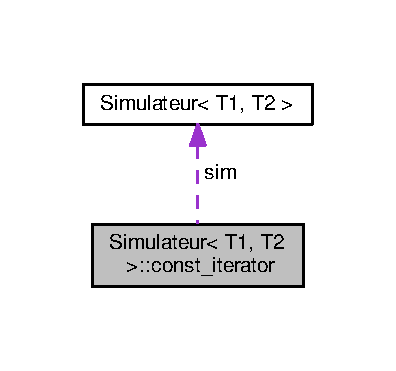
\includegraphics[width=190pt]{class_simulateur_1_1const__iterator__coll__graph}
\end{center}
\end{figure}
\subsection*{Fonctions membres publiques}
\begin{DoxyCompactItemize}
\item 
\hyperlink{class_simulateur_1_1const__iterator_adefd901a2eed44f15f00771cca1c940d}{const\+\_\+iterator} ()
\item 
\hyperlink{class_simulateur_1_1const__iterator}{const\+\_\+iterator} \& \hyperlink{class_simulateur_1_1const__iterator_ab5d1bea2f07780e6ae8d11a0accbfc87}{operator++} ()
\item 
const T2 \& \hyperlink{class_simulateur_1_1const__iterator_a4bc17b0d2decb5fb010155447f313c37}{operator$\ast$} () const 
\item 
bool \hyperlink{class_simulateur_1_1const__iterator_a1892ab7977db8b778365d94436652414}{operator!=} (\hyperlink{class_simulateur_1_1const__iterator}{const\+\_\+iterator} it) const 
\end{DoxyCompactItemize}
\subsection*{Fonctions membres privées}
\begin{DoxyCompactItemize}
\item 
\hyperlink{class_simulateur_1_1const__iterator_ac86b41f09bf9b8975b7f4d91ee5f0d52}{const\+\_\+iterator} (const \hyperlink{class_simulateur}{Simulateur} $\ast$s)
\item 
\hyperlink{class_simulateur_1_1const__iterator_a8baadf24b767532a6e5d3d4ed59e0eab}{const\+\_\+iterator} (const \hyperlink{class_simulateur}{Simulateur} $\ast$s, int dep)
\end{DoxyCompactItemize}
\subsection*{Attributs privés}
\begin{DoxyCompactItemize}
\item 
const \hyperlink{class_simulateur}{Simulateur} $\ast$ \hyperlink{class_simulateur_1_1const__iterator_af879bec3ae8b71f1c81826e0c1b24077}{sim}
\item 
int \hyperlink{class_simulateur_1_1const__iterator_aa4b2261e7087b7c68391c893aa531973}{i}
\end{DoxyCompactItemize}
\subsection*{Amis}
\begin{DoxyCompactItemize}
\item 
class \hyperlink{class_simulateur_1_1const__iterator_ae6c3966e699bf920c86e0bd006bd8183}{Simulateur}
\end{DoxyCompactItemize}


\subsection{Description détaillée}
\subsubsection*{template$<$class T1, class T2$>$\\*
class Simulateur$<$ T1, T2 $>$\+::const\+\_\+iterator}

permet le parcourt des états dans simulateur const 

\subsection{Documentation des constructeurs et destructeur}
\index{Simulateur\+::const\+\_\+iterator@{Simulateur\+::const\+\_\+iterator}!const\+\_\+iterator@{const\+\_\+iterator}}
\index{const\+\_\+iterator@{const\+\_\+iterator}!Simulateur\+::const\+\_\+iterator@{Simulateur\+::const\+\_\+iterator}}
\subsubsection[{\texorpdfstring{const\+\_\+iterator(const Simulateur $\ast$s)}{const_iterator(const Simulateur *s)}}]{\setlength{\rightskip}{0pt plus 5cm}template$<$class T1 , class T2 $>$ {\bf Simulateur}$<$ T1, T2 $>$\+::const\+\_\+iterator\+::const\+\_\+iterator (
\begin{DoxyParamCaption}
\item[{const {\bf Simulateur} $\ast$}]{s}
\end{DoxyParamCaption}
)\hspace{0.3cm}{\ttfamily [inline]}, {\ttfamily [private]}}\hypertarget{class_simulateur_1_1const__iterator_ac86b41f09bf9b8975b7f4d91ee5f0d52}{}\label{class_simulateur_1_1const__iterator_ac86b41f09bf9b8975b7f4d91ee5f0d52}
\index{Simulateur\+::const\+\_\+iterator@{Simulateur\+::const\+\_\+iterator}!const\+\_\+iterator@{const\+\_\+iterator}}
\index{const\+\_\+iterator@{const\+\_\+iterator}!Simulateur\+::const\+\_\+iterator@{Simulateur\+::const\+\_\+iterator}}
\subsubsection[{\texorpdfstring{const\+\_\+iterator(const Simulateur $\ast$s, int dep)}{const_iterator(const Simulateur *s, int dep)}}]{\setlength{\rightskip}{0pt plus 5cm}template$<$class T1 , class T2 $>$ {\bf Simulateur}$<$ T1, T2 $>$\+::const\+\_\+iterator\+::const\+\_\+iterator (
\begin{DoxyParamCaption}
\item[{const {\bf Simulateur} $\ast$}]{s, }
\item[{int}]{dep}
\end{DoxyParamCaption}
)\hspace{0.3cm}{\ttfamily [inline]}, {\ttfamily [private]}}\hypertarget{class_simulateur_1_1const__iterator_a8baadf24b767532a6e5d3d4ed59e0eab}{}\label{class_simulateur_1_1const__iterator_a8baadf24b767532a6e5d3d4ed59e0eab}
\index{Simulateur\+::const\+\_\+iterator@{Simulateur\+::const\+\_\+iterator}!const\+\_\+iterator@{const\+\_\+iterator}}
\index{const\+\_\+iterator@{const\+\_\+iterator}!Simulateur\+::const\+\_\+iterator@{Simulateur\+::const\+\_\+iterator}}
\subsubsection[{\texorpdfstring{const\+\_\+iterator()}{const_iterator()}}]{\setlength{\rightskip}{0pt plus 5cm}template$<$class T1 , class T2 $>$ {\bf Simulateur}$<$ T1, T2 $>$\+::const\+\_\+iterator\+::const\+\_\+iterator (
\begin{DoxyParamCaption}
{}
\end{DoxyParamCaption}
)\hspace{0.3cm}{\ttfamily [inline]}}\hypertarget{class_simulateur_1_1const__iterator_adefd901a2eed44f15f00771cca1c940d}{}\label{class_simulateur_1_1const__iterator_adefd901a2eed44f15f00771cca1c940d}


\subsection{Documentation des fonctions membres}
\index{Simulateur\+::const\+\_\+iterator@{Simulateur\+::const\+\_\+iterator}!operator"!=@{operator"!=}}
\index{operator"!=@{operator"!=}!Simulateur\+::const\+\_\+iterator@{Simulateur\+::const\+\_\+iterator}}
\subsubsection[{\texorpdfstring{operator"!=(const\+\_\+iterator it) const }{operator!=(const_iterator it) const }}]{\setlength{\rightskip}{0pt plus 5cm}template$<$class T1 , class T2 $>$ bool {\bf Simulateur}$<$ T1, T2 $>$\+::const\+\_\+iterator\+::operator!= (
\begin{DoxyParamCaption}
\item[{{\bf const\+\_\+iterator}}]{it}
\end{DoxyParamCaption}
) const\hspace{0.3cm}{\ttfamily [inline]}}\hypertarget{class_simulateur_1_1const__iterator_a1892ab7977db8b778365d94436652414}{}\label{class_simulateur_1_1const__iterator_a1892ab7977db8b778365d94436652414}
\index{Simulateur\+::const\+\_\+iterator@{Simulateur\+::const\+\_\+iterator}!operator$\ast$@{operator$\ast$}}
\index{operator$\ast$@{operator$\ast$}!Simulateur\+::const\+\_\+iterator@{Simulateur\+::const\+\_\+iterator}}
\subsubsection[{\texorpdfstring{operator$\ast$() const }{operator*() const }}]{\setlength{\rightskip}{0pt plus 5cm}template$<$class T1 , class T2 $>$ const T2\& {\bf Simulateur}$<$ T1, T2 $>$\+::const\+\_\+iterator\+::operator$\ast$ (
\begin{DoxyParamCaption}
{}
\end{DoxyParamCaption}
) const\hspace{0.3cm}{\ttfamily [inline]}}\hypertarget{class_simulateur_1_1const__iterator_a4bc17b0d2decb5fb010155447f313c37}{}\label{class_simulateur_1_1const__iterator_a4bc17b0d2decb5fb010155447f313c37}
\index{Simulateur\+::const\+\_\+iterator@{Simulateur\+::const\+\_\+iterator}!operator++@{operator++}}
\index{operator++@{operator++}!Simulateur\+::const\+\_\+iterator@{Simulateur\+::const\+\_\+iterator}}
\subsubsection[{\texorpdfstring{operator++()}{operator++()}}]{\setlength{\rightskip}{0pt plus 5cm}template$<$class T1 , class T2 $>$ {\bf const\+\_\+iterator}\& {\bf Simulateur}$<$ T1, T2 $>$\+::const\+\_\+iterator\+::operator++ (
\begin{DoxyParamCaption}
{}
\end{DoxyParamCaption}
)\hspace{0.3cm}{\ttfamily [inline]}}\hypertarget{class_simulateur_1_1const__iterator_ab5d1bea2f07780e6ae8d11a0accbfc87}{}\label{class_simulateur_1_1const__iterator_ab5d1bea2f07780e6ae8d11a0accbfc87}


\subsection{Documentation des fonctions amies et associées}
\index{Simulateur\+::const\+\_\+iterator@{Simulateur\+::const\+\_\+iterator}!Simulateur@{Simulateur}}
\index{Simulateur@{Simulateur}!Simulateur\+::const\+\_\+iterator@{Simulateur\+::const\+\_\+iterator}}
\subsubsection[{\texorpdfstring{Simulateur}{Simulateur}}]{\setlength{\rightskip}{0pt plus 5cm}template$<$class T1 , class T2 $>$ friend class {\bf Simulateur}\hspace{0.3cm}{\ttfamily [friend]}}\hypertarget{class_simulateur_1_1const__iterator_ae6c3966e699bf920c86e0bd006bd8183}{}\label{class_simulateur_1_1const__iterator_ae6c3966e699bf920c86e0bd006bd8183}


\subsection{Documentation des données membres}
\index{Simulateur\+::const\+\_\+iterator@{Simulateur\+::const\+\_\+iterator}!i@{i}}
\index{i@{i}!Simulateur\+::const\+\_\+iterator@{Simulateur\+::const\+\_\+iterator}}
\subsubsection[{\texorpdfstring{i}{i}}]{\setlength{\rightskip}{0pt plus 5cm}template$<$class T1 , class T2 $>$ int {\bf Simulateur}$<$ T1, T2 $>$\+::const\+\_\+iterator\+::i\hspace{0.3cm}{\ttfamily [private]}}\hypertarget{class_simulateur_1_1const__iterator_aa4b2261e7087b7c68391c893aa531973}{}\label{class_simulateur_1_1const__iterator_aa4b2261e7087b7c68391c893aa531973}
\index{Simulateur\+::const\+\_\+iterator@{Simulateur\+::const\+\_\+iterator}!sim@{sim}}
\index{sim@{sim}!Simulateur\+::const\+\_\+iterator@{Simulateur\+::const\+\_\+iterator}}
\subsubsection[{\texorpdfstring{sim}{sim}}]{\setlength{\rightskip}{0pt plus 5cm}template$<$class T1 , class T2 $>$ const {\bf Simulateur}$\ast$ {\bf Simulateur}$<$ T1, T2 $>$\+::const\+\_\+iterator\+::sim\hspace{0.3cm}{\ttfamily [private]}}\hypertarget{class_simulateur_1_1const__iterator_af879bec3ae8b71f1c81826e0c1b24077}{}\label{class_simulateur_1_1const__iterator_af879bec3ae8b71f1c81826e0c1b24077}


La documentation de cette classe a été générée à partir du fichier suivant \+:\begin{DoxyCompactItemize}
\item 
/home/thomaspaita/\+Bureau/info/\+L\+O21/\+L\+O21/\+Auto\+Cell/\hyperlink{_simulateur_8h}{Simulateur.\+h}\end{DoxyCompactItemize}

\hypertarget{class_etat}{}\section{Référence de la classe Etat}
\label{class_etat}\index{Etat@{Etat}}


Classe abstraite. La classe permet de généraliser un \hyperlink{class_etat}{Etat}.  




{\ttfamily \#include $<$Etat.\+h$>$}



Graphe d\textquotesingle{}héritage de Etat\+:
\nopagebreak
\begin{figure}[H]
\begin{center}
\leavevmode
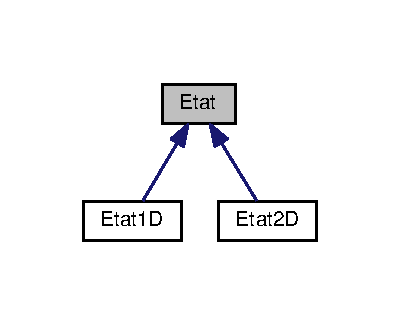
\includegraphics[width=192pt]{class_etat__inherit__graph}
\end{center}
\end{figure}
\subsection*{Fonctions membres publiques}
\begin{DoxyCompactItemize}
\item 
\hyperlink{class_etat_a78a5538e285af98cc010c0a197b14d50}{Etat} (unsigned int nb\+Cel, unsigned int nb\+Etat=2)
\begin{DoxyCompactList}\small\item\em Constructeur. \end{DoxyCompactList}\item 
virtual \hyperlink{class_etat_a00bde3e769da5523e194a780ca95f7f7}{$\sim$\+Etat} ()
\begin{DoxyCompactList}\small\item\em Destructeur. \end{DoxyCompactList}\item 
unsigned int \hyperlink{class_etat_ad7822bc39dbe59ce5123bebcecb5c311}{get\+Largeur} () const 
\begin{DoxyCompactList}\small\item\em Accesseur en lecture. \end{DoxyCompactList}\item 
void \hyperlink{class_etat_a42eb8dc32d9865c25ff34f011d2c2706}{set\+Largeur} (unsigned int l)
\begin{DoxyCompactList}\small\item\em change la largeur \end{DoxyCompactList}\item 
unsigned int \hyperlink{class_etat_a9d4366197c4c39da8dd77929c4ca9621}{get\+Nb\+Etat} () const 
\begin{DoxyCompactList}\small\item\em Accesseur en lecture. \end{DoxyCompactList}\item 
virtual unsigned int \hyperlink{class_etat_aa2eeed5ffbef3b53a149385f81bf2af0}{get\+Hauteur} () const =0
\begin{DoxyCompactList}\small\item\em Accesseur en lecture méthode virtuelle pure. \end{DoxyCompactList}\item 
virtual void \hyperlink{class_etat_ac29c6d30fc8c982ff5f67eab6fc396de}{adjust\+Etat} ()=0
\begin{DoxyCompactList}\small\item\em Ajuste la taille de l\textquotesingle{}état méthode virtuelle pure. \end{DoxyCompactList}\item 
virtual void \hyperlink{class_etat_a796cef1d7607e3d185bec0a31eb7a819}{afficher} () const =0
\begin{DoxyCompactList}\small\item\em affiche un état dans la sortier standard méthode virtuelle pure \end{DoxyCompactList}\end{DoxyCompactItemize}
\subsection*{Attributs protégés}
\begin{DoxyCompactItemize}
\item 
unsigned int \hyperlink{class_etat_af575fb141b3c300c9cbb61337094ba1b}{m\+\_\+largeur}
\item 
unsigned int \hyperlink{class_etat_a281d9e6224c108d5db463540bb2414f3}{m\+\_\+nb\+Etat}
\end{DoxyCompactItemize}


\subsection{Description détaillée}
Classe abstraite. La classe permet de généraliser un \hyperlink{class_etat}{Etat}. 

\subsection{Documentation des constructeurs et destructeur}
\index{Etat@{Etat}!Etat@{Etat}}
\index{Etat@{Etat}!Etat@{Etat}}
\subsubsection[{\texorpdfstring{Etat(unsigned int nb\+Cel, unsigned int nb\+Etat=2)}{Etat(unsigned int nbCel, unsigned int nbEtat=2)}}]{\setlength{\rightskip}{0pt plus 5cm}Etat\+::\+Etat (
\begin{DoxyParamCaption}
\item[{unsigned int}]{nb\+Cel, }
\item[{unsigned int}]{nb\+Etat = {\ttfamily 2}}
\end{DoxyParamCaption}
)\hspace{0.3cm}{\ttfamily [inline]}}\hypertarget{class_etat_a78a5538e285af98cc010c0a197b14d50}{}\label{class_etat_a78a5538e285af98cc010c0a197b14d50}


Constructeur. 


\begin{DoxyParams}{Paramètres}
{\em nb\+Cel} & \+: largeur\+: unsigned int \\
\hline
{\em nb\+Etat} & \+: nombre d\textquotesingle{}état \+:unsigned int \\
\hline
\end{DoxyParams}
\index{Etat@{Etat}!````~Etat@{$\sim$\+Etat}}
\index{````~Etat@{$\sim$\+Etat}!Etat@{Etat}}
\subsubsection[{\texorpdfstring{$\sim$\+Etat()}{~Etat()}}]{\setlength{\rightskip}{0pt plus 5cm}virtual Etat\+::$\sim$\+Etat (
\begin{DoxyParamCaption}
{}
\end{DoxyParamCaption}
)\hspace{0.3cm}{\ttfamily [inline]}, {\ttfamily [virtual]}}\hypertarget{class_etat_a00bde3e769da5523e194a780ca95f7f7}{}\label{class_etat_a00bde3e769da5523e194a780ca95f7f7}


Destructeur. 



\subsection{Documentation des fonctions membres}
\index{Etat@{Etat}!adjust\+Etat@{adjust\+Etat}}
\index{adjust\+Etat@{adjust\+Etat}!Etat@{Etat}}
\subsubsection[{\texorpdfstring{adjust\+Etat()=0}{adjustEtat()=0}}]{\setlength{\rightskip}{0pt plus 5cm}virtual void Etat\+::adjust\+Etat (
\begin{DoxyParamCaption}
{}
\end{DoxyParamCaption}
)\hspace{0.3cm}{\ttfamily [pure virtual]}}\hypertarget{class_etat_ac29c6d30fc8c982ff5f67eab6fc396de}{}\label{class_etat_ac29c6d30fc8c982ff5f67eab6fc396de}


Ajuste la taille de l\textquotesingle{}état méthode virtuelle pure. 



Implémenté dans \hyperlink{class_etat1_d_a95f0f0455d3dfda771330648ec5395fb}{Etat1D}, et \hyperlink{class_etat2_d_af99e5b4041ce363a4b1e96a6751719d5}{Etat2D}.

\index{Etat@{Etat}!afficher@{afficher}}
\index{afficher@{afficher}!Etat@{Etat}}
\subsubsection[{\texorpdfstring{afficher() const =0}{afficher() const =0}}]{\setlength{\rightskip}{0pt plus 5cm}virtual void Etat\+::afficher (
\begin{DoxyParamCaption}
{}
\end{DoxyParamCaption}
) const\hspace{0.3cm}{\ttfamily [pure virtual]}}\hypertarget{class_etat_a796cef1d7607e3d185bec0a31eb7a819}{}\label{class_etat_a796cef1d7607e3d185bec0a31eb7a819}


affiche un état dans la sortier standard méthode virtuelle pure 



Implémenté dans \hyperlink{class_etat1_d_a11b2e64dc835aad04a5f138337ba7b99}{Etat1D}, et \hyperlink{class_etat2_d_a6fa30b43d2971b01cbfb59aef094aded}{Etat2D}.

\index{Etat@{Etat}!get\+Hauteur@{get\+Hauteur}}
\index{get\+Hauteur@{get\+Hauteur}!Etat@{Etat}}
\subsubsection[{\texorpdfstring{get\+Hauteur() const =0}{getHauteur() const =0}}]{\setlength{\rightskip}{0pt plus 5cm}virtual unsigned int Etat\+::get\+Hauteur (
\begin{DoxyParamCaption}
{}
\end{DoxyParamCaption}
) const\hspace{0.3cm}{\ttfamily [pure virtual]}}\hypertarget{class_etat_aa2eeed5ffbef3b53a149385f81bf2af0}{}\label{class_etat_aa2eeed5ffbef3b53a149385f81bf2af0}


Accesseur en lecture méthode virtuelle pure. 



Implémenté dans \hyperlink{class_etat1_d_aed8c9082f8caefeef7687ba1f4590f40}{Etat1D}, et \hyperlink{class_etat2_d_aff82bb61adbe51f2702e34f0ea34a55d}{Etat2D}.

\index{Etat@{Etat}!get\+Largeur@{get\+Largeur}}
\index{get\+Largeur@{get\+Largeur}!Etat@{Etat}}
\subsubsection[{\texorpdfstring{get\+Largeur() const }{getLargeur() const }}]{\setlength{\rightskip}{0pt plus 5cm}unsigned int Etat\+::get\+Largeur (
\begin{DoxyParamCaption}
{}
\end{DoxyParamCaption}
) const\hspace{0.3cm}{\ttfamily [inline]}}\hypertarget{class_etat_ad7822bc39dbe59ce5123bebcecb5c311}{}\label{class_etat_ad7822bc39dbe59ce5123bebcecb5c311}


Accesseur en lecture. 

\begin{DoxyReturn}{Renvoie}
m\+\_\+largeur \+: unsigned int 
\end{DoxyReturn}
\index{Etat@{Etat}!get\+Nb\+Etat@{get\+Nb\+Etat}}
\index{get\+Nb\+Etat@{get\+Nb\+Etat}!Etat@{Etat}}
\subsubsection[{\texorpdfstring{get\+Nb\+Etat() const }{getNbEtat() const }}]{\setlength{\rightskip}{0pt plus 5cm}unsigned int Etat\+::get\+Nb\+Etat (
\begin{DoxyParamCaption}
{}
\end{DoxyParamCaption}
) const\hspace{0.3cm}{\ttfamily [inline]}}\hypertarget{class_etat_a9d4366197c4c39da8dd77929c4ca9621}{}\label{class_etat_a9d4366197c4c39da8dd77929c4ca9621}


Accesseur en lecture. 

\begin{DoxyReturn}{Renvoie}
m\+\_\+nb\+Etat \+: unsigned int 
\end{DoxyReturn}
\index{Etat@{Etat}!set\+Largeur@{set\+Largeur}}
\index{set\+Largeur@{set\+Largeur}!Etat@{Etat}}
\subsubsection[{\texorpdfstring{set\+Largeur(unsigned int l)}{setLargeur(unsigned int l)}}]{\setlength{\rightskip}{0pt plus 5cm}void Etat\+::set\+Largeur (
\begin{DoxyParamCaption}
\item[{unsigned int}]{l}
\end{DoxyParamCaption}
)\hspace{0.3cm}{\ttfamily [inline]}}\hypertarget{class_etat_a42eb8dc32d9865c25ff34f011d2c2706}{}\label{class_etat_a42eb8dc32d9865c25ff34f011d2c2706}


change la largeur 


\begin{DoxyParams}{Paramètres}
{\em l} & \+: nouvelle largeur \+:unsigned int \\
\hline
\end{DoxyParams}


\subsection{Documentation des données membres}
\index{Etat@{Etat}!m\+\_\+largeur@{m\+\_\+largeur}}
\index{m\+\_\+largeur@{m\+\_\+largeur}!Etat@{Etat}}
\subsubsection[{\texorpdfstring{m\+\_\+largeur}{m_largeur}}]{\setlength{\rightskip}{0pt plus 5cm}unsigned int Etat\+::m\+\_\+largeur\hspace{0.3cm}{\ttfamily [protected]}}\hypertarget{class_etat_af575fb141b3c300c9cbb61337094ba1b}{}\label{class_etat_af575fb141b3c300c9cbb61337094ba1b}
largeur de l\textquotesingle{}état \index{Etat@{Etat}!m\+\_\+nb\+Etat@{m\+\_\+nb\+Etat}}
\index{m\+\_\+nb\+Etat@{m\+\_\+nb\+Etat}!Etat@{Etat}}
\subsubsection[{\texorpdfstring{m\+\_\+nb\+Etat}{m_nbEtat}}]{\setlength{\rightskip}{0pt plus 5cm}unsigned int Etat\+::m\+\_\+nb\+Etat\hspace{0.3cm}{\ttfamily [protected]}}\hypertarget{class_etat_a281d9e6224c108d5db463540bb2414f3}{}\label{class_etat_a281d9e6224c108d5db463540bb2414f3}
nombre d\textquotesingle{}état d\textquotesingle{}une cellule 

La documentation de cette classe a été générée à partir du fichier suivant \+:\begin{DoxyCompactItemize}
\item 
info/\+L\+O21/\+L\+O21/\+Auto\+Cell/\hyperlink{_etat_8h}{Etat.\+h}\end{DoxyCompactItemize}

\hypertarget{class_etat1_d}{}\section{Référence de la classe Etat1D}
\label{class_etat1_d}\index{Etat1D@{Etat1D}}


hérite de \hyperlink{class_etat}{Etat}. Permet de créer de état à 1\+Dimension  




{\ttfamily \#include $<$Etat1\+D.\+h$>$}



Graphe d\textquotesingle{}héritage de Etat1D\+:
\nopagebreak
\begin{figure}[H]
\begin{center}
\leavevmode
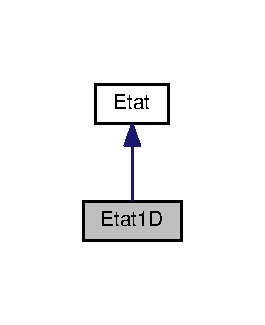
\includegraphics[width=127pt]{class_etat1_d__inherit__graph}
\end{center}
\end{figure}


Graphe de collaboration de Etat1D\+:
\nopagebreak
\begin{figure}[H]
\begin{center}
\leavevmode
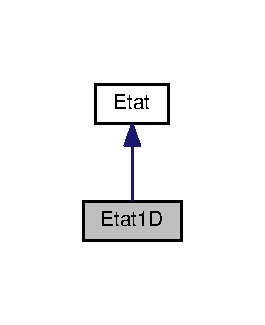
\includegraphics[width=127pt]{class_etat1_d__coll__graph}
\end{center}
\end{figure}
\subsection*{Fonctions membres publiques}
\begin{DoxyCompactItemize}
\item 
\hyperlink{class_etat1_d_ae9cabf1b4a858c1c0c458387b52a8ce4}{Etat1D} (unsigned int taille=0, unsigned int nb\+Etat=2)
\begin{DoxyCompactList}\small\item\em Constructeur. \end{DoxyCompactList}\item 
\hyperlink{class_etat1_d_a1294037bb4f90d1da9deb872caa2cbe9}{Etat1D} (\hyperlink{class_etat1_d}{Etat1D} const \&etat)
\begin{DoxyCompactList}\small\item\em Constructeur par recopie. \end{DoxyCompactList}\item 
virtual \hyperlink{class_etat1_d_aba338e321568e641e7c3d4e9ef5e13e7}{$\sim$\+Etat1D} ()
\begin{DoxyCompactList}\small\item\em Destructeur. \end{DoxyCompactList}\item 
unsigned int \hyperlink{class_etat1_d_ab34b895c79fecfb41fac13e180c13302}{get\+Dimension} () const 
\begin{DoxyCompactList}\small\item\em accesseur lecture \end{DoxyCompactList}\item 
bool \hyperlink{class_etat1_d_a4a969863ec0067872148b326cea0cf4e}{get\+Cellule} (unsigned int i) const 
\begin{DoxyCompactList}\small\item\em accesseur lecture \end{DoxyCompactList}\item 
void \hyperlink{class_etat1_d_a04dc19eb1adbfe392eff45c7c5880c74}{set\+Cellule} (unsigned int i, bool val)
\begin{DoxyCompactList}\small\item\em accesseur écriture \end{DoxyCompactList}\item 
void \hyperlink{class_etat1_d_a11b2e64dc835aad04a5f138337ba7b99}{afficher} () const 
\begin{DoxyCompactList}\small\item\em affiche un \hyperlink{class_etat1_d}{Etat1D} \end{DoxyCompactList}\item 
\hyperlink{class_etat1_d}{Etat1D} \& \hyperlink{class_etat1_d_a4ce3b4931c766b2a6cdf6e3ac7590c5a}{operator=} (const \hyperlink{class_etat1_d}{Etat1D} \&etat)
\begin{DoxyCompactList}\small\item\em operateur de copie \end{DoxyCompactList}\item 
virtual unsigned int \hyperlink{class_etat1_d_aed8c9082f8caefeef7687ba1f4590f40}{get\+Hauteur} () const 
\begin{DoxyCompactList}\small\item\em méthode virtuelle \end{DoxyCompactList}\item 
virtual void \hyperlink{class_etat1_d_a95f0f0455d3dfda771330648ec5395fb}{adjust\+Etat} ()
\begin{DoxyCompactList}\small\item\em méthode virtuelle modifie la taille de l\textquotesingle{}état \end{DoxyCompactList}\end{DoxyCompactItemize}
\subsection*{Attributs protégés}
\begin{DoxyCompactItemize}
\item 
std\+::vector$<$ bool $>$ \hyperlink{class_etat1_d_a07068969d6d83e95a8d04363914adf33}{m\+\_\+tab}
\end{DoxyCompactItemize}
\subsection*{Amis}
\begin{DoxyCompactItemize}
\item 
class \hyperlink{class_etat1_d_a7b442c5e6a2ad84fcc725706d1f77dfe}{Automate1D}
\end{DoxyCompactItemize}


\subsection{Description détaillée}
hérite de \hyperlink{class_etat}{Etat}. Permet de créer de état à 1\+Dimension 

\subsection{Documentation des constructeurs et destructeur}
\index{Etat1D@{Etat1D}!Etat1D@{Etat1D}}
\index{Etat1D@{Etat1D}!Etat1D@{Etat1D}}
\subsubsection[{\texorpdfstring{Etat1\+D(unsigned int taille=0, unsigned int nb\+Etat=2)}{Etat1D(unsigned int taille=0, unsigned int nbEtat=2)}}]{\setlength{\rightskip}{0pt plus 5cm}Etat1\+D\+::\+Etat1D (
\begin{DoxyParamCaption}
\item[{unsigned int}]{taille = {\ttfamily 0}, }
\item[{unsigned int}]{nb\+Etat = {\ttfamily 2}}
\end{DoxyParamCaption}
)}\hypertarget{class_etat1_d_ae9cabf1b4a858c1c0c458387b52a8ce4}{}\label{class_etat1_d_ae9cabf1b4a858c1c0c458387b52a8ce4}


Constructeur. 


\begin{DoxyParams}{Paramètres}
{\em taille} & \+: nombre de cellule \+: unsigned int \\
\hline
{\em nb\+Etat} & \+: unsigned int \\
\hline
\end{DoxyParams}
\index{Etat1D@{Etat1D}!Etat1D@{Etat1D}}
\index{Etat1D@{Etat1D}!Etat1D@{Etat1D}}
\subsubsection[{\texorpdfstring{Etat1\+D(\+Etat1\+D const \&etat)}{Etat1D(Etat1D const &etat)}}]{\setlength{\rightskip}{0pt plus 5cm}Etat1\+D\+::\+Etat1D (
\begin{DoxyParamCaption}
\item[{{\bf Etat1D} const \&}]{etat}
\end{DoxyParamCaption}
)}\hypertarget{class_etat1_d_a1294037bb4f90d1da9deb872caa2cbe9}{}\label{class_etat1_d_a1294037bb4f90d1da9deb872caa2cbe9}


Constructeur par recopie. 

\index{Etat1D@{Etat1D}!````~Etat1D@{$\sim$\+Etat1D}}
\index{````~Etat1D@{$\sim$\+Etat1D}!Etat1D@{Etat1D}}
\subsubsection[{\texorpdfstring{$\sim$\+Etat1\+D()}{~Etat1D()}}]{\setlength{\rightskip}{0pt plus 5cm}virtual Etat1\+D\+::$\sim$\+Etat1D (
\begin{DoxyParamCaption}
{}
\end{DoxyParamCaption}
)\hspace{0.3cm}{\ttfamily [inline]}, {\ttfamily [virtual]}}\hypertarget{class_etat1_d_aba338e321568e641e7c3d4e9ef5e13e7}{}\label{class_etat1_d_aba338e321568e641e7c3d4e9ef5e13e7}


Destructeur. 



\subsection{Documentation des fonctions membres}
\index{Etat1D@{Etat1D}!adjust\+Etat@{adjust\+Etat}}
\index{adjust\+Etat@{adjust\+Etat}!Etat1D@{Etat1D}}
\subsubsection[{\texorpdfstring{adjust\+Etat()}{adjustEtat()}}]{\setlength{\rightskip}{0pt plus 5cm}virtual void Etat1\+D\+::adjust\+Etat (
\begin{DoxyParamCaption}
{}
\end{DoxyParamCaption}
)\hspace{0.3cm}{\ttfamily [inline]}, {\ttfamily [virtual]}}\hypertarget{class_etat1_d_a95f0f0455d3dfda771330648ec5395fb}{}\label{class_etat1_d_a95f0f0455d3dfda771330648ec5395fb}


méthode virtuelle modifie la taille de l\textquotesingle{}état 



Implémente \hyperlink{class_etat_ac29c6d30fc8c982ff5f67eab6fc396de}{Etat}.

\index{Etat1D@{Etat1D}!afficher@{afficher}}
\index{afficher@{afficher}!Etat1D@{Etat1D}}
\subsubsection[{\texorpdfstring{afficher() const }{afficher() const }}]{\setlength{\rightskip}{0pt plus 5cm}void Etat1\+D\+::afficher (
\begin{DoxyParamCaption}
{}
\end{DoxyParamCaption}
) const\hspace{0.3cm}{\ttfamily [inline]}, {\ttfamily [virtual]}}\hypertarget{class_etat1_d_a11b2e64dc835aad04a5f138337ba7b99}{}\label{class_etat1_d_a11b2e64dc835aad04a5f138337ba7b99}


affiche un \hyperlink{class_etat1_d}{Etat1D} 



Implémente \hyperlink{class_etat_a796cef1d7607e3d185bec0a31eb7a819}{Etat}.

\index{Etat1D@{Etat1D}!get\+Cellule@{get\+Cellule}}
\index{get\+Cellule@{get\+Cellule}!Etat1D@{Etat1D}}
\subsubsection[{\texorpdfstring{get\+Cellule(unsigned int i) const }{getCellule(unsigned int i) const }}]{\setlength{\rightskip}{0pt plus 5cm}bool Etat1\+D\+::get\+Cellule (
\begin{DoxyParamCaption}
\item[{unsigned int}]{i}
\end{DoxyParamCaption}
) const}\hypertarget{class_etat1_d_a4a969863ec0067872148b326cea0cf4e}{}\label{class_etat1_d_a4a969863ec0067872148b326cea0cf4e}


accesseur lecture 


\begin{DoxyParams}{Paramètres}
{\em i} & \+: indice \+:unsigned int \\
\hline
\end{DoxyParams}
\begin{DoxyReturn}{Renvoie}
valeur \+: bool 
\end{DoxyReturn}
\index{Etat1D@{Etat1D}!get\+Dimension@{get\+Dimension}}
\index{get\+Dimension@{get\+Dimension}!Etat1D@{Etat1D}}
\subsubsection[{\texorpdfstring{get\+Dimension() const }{getDimension() const }}]{\setlength{\rightskip}{0pt plus 5cm}unsigned int Etat1\+D\+::get\+Dimension (
\begin{DoxyParamCaption}
{}
\end{DoxyParamCaption}
) const}\hypertarget{class_etat1_d_ab34b895c79fecfb41fac13e180c13302}{}\label{class_etat1_d_ab34b895c79fecfb41fac13e180c13302}


accesseur lecture 

\begin{DoxyReturn}{Renvoie}
taille \+: unsigned int 
\end{DoxyReturn}
\index{Etat1D@{Etat1D}!get\+Hauteur@{get\+Hauteur}}
\index{get\+Hauteur@{get\+Hauteur}!Etat1D@{Etat1D}}
\subsubsection[{\texorpdfstring{get\+Hauteur() const }{getHauteur() const }}]{\setlength{\rightskip}{0pt plus 5cm}virtual unsigned int Etat1\+D\+::get\+Hauteur (
\begin{DoxyParamCaption}
{}
\end{DoxyParamCaption}
) const\hspace{0.3cm}{\ttfamily [inline]}, {\ttfamily [virtual]}}\hypertarget{class_etat1_d_aed8c9082f8caefeef7687ba1f4590f40}{}\label{class_etat1_d_aed8c9082f8caefeef7687ba1f4590f40}


méthode virtuelle 


\begin{DoxyParams}{Paramètres}
{\em etat} & \+: const \hyperlink{class_etat1_d}{Etat1D}\&l \\
\hline
\end{DoxyParams}
\begin{DoxyReturn}{Renvoie}
\hyperlink{class_etat1_d}{Etat1D}\& 
\end{DoxyReturn}


Implémente \hyperlink{class_etat_aa2eeed5ffbef3b53a149385f81bf2af0}{Etat}.

\index{Etat1D@{Etat1D}!operator=@{operator=}}
\index{operator=@{operator=}!Etat1D@{Etat1D}}
\subsubsection[{\texorpdfstring{operator=(const Etat1\+D \&etat)}{operator=(const Etat1D &etat)}}]{\setlength{\rightskip}{0pt plus 5cm}{\bf Etat1D} \& Etat1\+D\+::operator= (
\begin{DoxyParamCaption}
\item[{const {\bf Etat1D} \&}]{etat}
\end{DoxyParamCaption}
)}\hypertarget{class_etat1_d_a4ce3b4931c766b2a6cdf6e3ac7590c5a}{}\label{class_etat1_d_a4ce3b4931c766b2a6cdf6e3ac7590c5a}


operateur de copie 


\begin{DoxyParams}{Paramètres}
{\em etat} & \+: const \hyperlink{class_etat1_d}{Etat1D}\&l \\
\hline
\end{DoxyParams}
\begin{DoxyReturn}{Renvoie}
\hyperlink{class_etat1_d}{Etat1D}\& 
\end{DoxyReturn}
\index{Etat1D@{Etat1D}!set\+Cellule@{set\+Cellule}}
\index{set\+Cellule@{set\+Cellule}!Etat1D@{Etat1D}}
\subsubsection[{\texorpdfstring{set\+Cellule(unsigned int i, bool val)}{setCellule(unsigned int i, bool val)}}]{\setlength{\rightskip}{0pt plus 5cm}void Etat1\+D\+::set\+Cellule (
\begin{DoxyParamCaption}
\item[{unsigned int}]{i, }
\item[{bool}]{val}
\end{DoxyParamCaption}
)}\hypertarget{class_etat1_d_a04dc19eb1adbfe392eff45c7c5880c74}{}\label{class_etat1_d_a04dc19eb1adbfe392eff45c7c5880c74}


accesseur écriture 


\begin{DoxyParams}{Paramètres}
{\em i} & \+: indice \+:unsigned int \\
\hline
{\em val} & \+: valeur \+: bool \\
\hline
\end{DoxyParams}


\subsection{Documentation des fonctions amies et associées}
\index{Etat1D@{Etat1D}!Automate1D@{Automate1D}}
\index{Automate1D@{Automate1D}!Etat1D@{Etat1D}}
\subsubsection[{\texorpdfstring{Automate1D}{Automate1D}}]{\setlength{\rightskip}{0pt plus 5cm}friend class {\bf Automate1D}\hspace{0.3cm}{\ttfamily [friend]}}\hypertarget{class_etat1_d_a7b442c5e6a2ad84fcc725706d1f77dfe}{}\label{class_etat1_d_a7b442c5e6a2ad84fcc725706d1f77dfe}


\subsection{Documentation des données membres}
\index{Etat1D@{Etat1D}!m\+\_\+tab@{m\+\_\+tab}}
\index{m\+\_\+tab@{m\+\_\+tab}!Etat1D@{Etat1D}}
\subsubsection[{\texorpdfstring{m\+\_\+tab}{m_tab}}]{\setlength{\rightskip}{0pt plus 5cm}std\+::vector$<$bool$>$ Etat1\+D\+::m\+\_\+tab\hspace{0.3cm}{\ttfamily [protected]}}\hypertarget{class_etat1_d_a07068969d6d83e95a8d04363914adf33}{}\label{class_etat1_d_a07068969d6d83e95a8d04363914adf33}
\hyperlink{class_etat}{Etat} de la cellule 

La documentation de cette classe a été générée à partir des fichiers suivants \+:\begin{DoxyCompactItemize}
\item 
info/\+L\+O21/\+L\+O21/\+Auto\+Cell/\hyperlink{_etat1_d_8h}{Etat1\+D.\+h}\item 
info/\+L\+O21/\+L\+O21/\+Auto\+Cell/\hyperlink{_etat1_d_8cpp}{Etat1\+D.\+cpp}\end{DoxyCompactItemize}

\hypertarget{class_etat2_d}{}\section{Référence de la classe Etat2D}
\label{class_etat2_d}\index{Etat2D@{Etat2D}}


hérite de \hyperlink{class_etat}{Etat}. Permet de créer des états à 2 dimensions  




{\ttfamily \#include $<$Etat2\+D.\+h$>$}



Graphe d\textquotesingle{}héritage de Etat2D\+:
\nopagebreak
\begin{figure}[H]
\begin{center}
\leavevmode
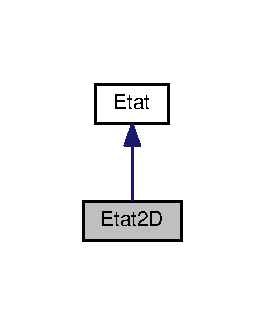
\includegraphics[width=127pt]{class_etat2_d__inherit__graph}
\end{center}
\end{figure}


Graphe de collaboration de Etat2D\+:
\nopagebreak
\begin{figure}[H]
\begin{center}
\leavevmode
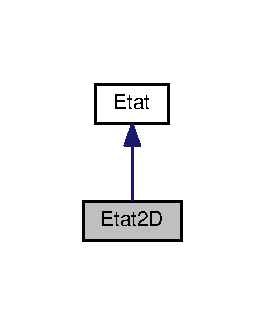
\includegraphics[width=127pt]{class_etat2_d__coll__graph}
\end{center}
\end{figure}
\subsection*{Fonctions membres publiques}
\begin{DoxyCompactItemize}
\item 
\hyperlink{class_etat2_d_aae67a6ba3b3b3726a9533f647d34dd55}{Etat2D} (unsigned int l=0, unsigned int h=0, unsigned int nb\+Etat=2)
\begin{DoxyCompactList}\small\item\em Constructeur. \end{DoxyCompactList}\item 
\hyperlink{class_etat2_d_a3eaa7f0e606a9b2f5fc634d6b571042e}{$\sim$\+Etat2D} ()
\begin{DoxyCompactList}\small\item\em Destructeur. \end{DoxyCompactList}\item 
unsigned int \hyperlink{class_etat2_d_aff82bb61adbe51f2702e34f0ea34a55d}{get\+Hauteur} () const 
\begin{DoxyCompactList}\small\item\em Accesseur en lecture. \end{DoxyCompactList}\item 
void \hyperlink{class_etat2_d_a97b757ecf3f703f5e418c00e250c074c}{set\+Hauteur} (unsigned int h)
\begin{DoxyCompactList}\small\item\em modifie la hauteur \end{DoxyCompactList}\item 
void \hyperlink{class_etat2_d_a6fa30b43d2971b01cbfb59aef094aded}{afficher} () const 
\begin{DoxyCompactList}\small\item\em affiche l\textquotesingle{}état \end{DoxyCompactList}\item 
void \hyperlink{class_etat2_d_a96f855c00941ce59b2c84d347dfb5e1c}{set\+Cellule} (unsigned int i, unsigned int j, unsigned short int val)
\begin{DoxyCompactList}\small\item\em modifie la valeur d\textquotesingle{}une cellule \end{DoxyCompactList}\item 
unsigned short int \hyperlink{class_etat2_d_adfe7448075788e3cd17c0b7df50b9438}{get\+Cellule} (unsigned int i, unsigned int j) const 
\begin{DoxyCompactList}\small\item\em Accesseur en lecture. \end{DoxyCompactList}\item 
virtual void \hyperlink{class_etat2_d_af99e5b4041ce363a4b1e96a6751719d5}{adjust\+Etat} ()
\begin{DoxyCompactList}\small\item\em ajuste la taille de l\textquotesingle{}etat \end{DoxyCompactList}\item 
bool \hyperlink{class_etat2_d_a6834241d99725640691eb3a252d14f5a}{operator==} (const \hyperlink{class_etat2_d}{Etat2D} \&e) const 
\begin{DoxyCompactList}\small\item\em opérateur d\textquotesingle{}affectation \end{DoxyCompactList}\end{DoxyCompactItemize}
\subsection*{Attributs protégés}
\begin{DoxyCompactItemize}
\item 
std\+::vector$<$ std\+::vector$<$ unsigned short int $>$ $>$ \hyperlink{class_etat2_d_a82d1c6326dedc79f902c1782d6a10cfb}{m\+\_\+valeur}
\item 
unsigned int \hyperlink{class_etat2_d_a9be83a06c967b20b80b344e50af02626}{m\+\_\+hauteur}
\end{DoxyCompactItemize}


\subsection{Description détaillée}
hérite de \hyperlink{class_etat}{Etat}. Permet de créer des états à 2 dimensions 

\subsection{Documentation des constructeurs et destructeur}
\index{Etat2D@{Etat2D}!Etat2D@{Etat2D}}
\index{Etat2D@{Etat2D}!Etat2D@{Etat2D}}
\subsubsection[{\texorpdfstring{Etat2\+D(unsigned int l=0, unsigned int h=0, unsigned int nb\+Etat=2)}{Etat2D(unsigned int l=0, unsigned int h=0, unsigned int nbEtat=2)}}]{\setlength{\rightskip}{0pt plus 5cm}Etat2\+D\+::\+Etat2D (
\begin{DoxyParamCaption}
\item[{unsigned int}]{l = {\ttfamily 0}, }
\item[{unsigned int}]{h = {\ttfamily 0}, }
\item[{unsigned int}]{nb\+Etat = {\ttfamily 2}}
\end{DoxyParamCaption}
)\hspace{0.3cm}{\ttfamily [inline]}}\hypertarget{class_etat2_d_aae67a6ba3b3b3726a9533f647d34dd55}{}\label{class_etat2_d_aae67a6ba3b3b3726a9533f647d34dd55}


Constructeur. 


\begin{DoxyParams}{Paramètres}
{\em l} & \+: largeur \+: unsigned int \\
\hline
{\em h} & \+: hauteur\+: unsigned int \\
\hline
{\em nb\+Etat} & \+: nombre d\textquotesingle{}état \+:unsigned int \\
\hline
\end{DoxyParams}
\index{Etat2D@{Etat2D}!````~Etat2D@{$\sim$\+Etat2D}}
\index{````~Etat2D@{$\sim$\+Etat2D}!Etat2D@{Etat2D}}
\subsubsection[{\texorpdfstring{$\sim$\+Etat2\+D()}{~Etat2D()}}]{\setlength{\rightskip}{0pt plus 5cm}Etat2\+D\+::$\sim$\+Etat2D (
\begin{DoxyParamCaption}
{}
\end{DoxyParamCaption}
)\hspace{0.3cm}{\ttfamily [inline]}}\hypertarget{class_etat2_d_a3eaa7f0e606a9b2f5fc634d6b571042e}{}\label{class_etat2_d_a3eaa7f0e606a9b2f5fc634d6b571042e}


Destructeur. 



\subsection{Documentation des fonctions membres}
\index{Etat2D@{Etat2D}!adjust\+Etat@{adjust\+Etat}}
\index{adjust\+Etat@{adjust\+Etat}!Etat2D@{Etat2D}}
\subsubsection[{\texorpdfstring{adjust\+Etat()}{adjustEtat()}}]{\setlength{\rightskip}{0pt plus 5cm}void Etat2\+D\+::adjust\+Etat (
\begin{DoxyParamCaption}
{}
\end{DoxyParamCaption}
)\hspace{0.3cm}{\ttfamily [virtual]}}\hypertarget{class_etat2_d_af99e5b4041ce363a4b1e96a6751719d5}{}\label{class_etat2_d_af99e5b4041ce363a4b1e96a6751719d5}


ajuste la taille de l\textquotesingle{}etat 



Implémente \hyperlink{class_etat_ac29c6d30fc8c982ff5f67eab6fc396de}{Etat}.

\index{Etat2D@{Etat2D}!afficher@{afficher}}
\index{afficher@{afficher}!Etat2D@{Etat2D}}
\subsubsection[{\texorpdfstring{afficher() const }{afficher() const }}]{\setlength{\rightskip}{0pt plus 5cm}void Etat2\+D\+::afficher (
\begin{DoxyParamCaption}
{}
\end{DoxyParamCaption}
) const\hspace{0.3cm}{\ttfamily [virtual]}}\hypertarget{class_etat2_d_a6fa30b43d2971b01cbfb59aef094aded}{}\label{class_etat2_d_a6fa30b43d2971b01cbfb59aef094aded}


affiche l\textquotesingle{}état 



Implémente \hyperlink{class_etat_a796cef1d7607e3d185bec0a31eb7a819}{Etat}.

\index{Etat2D@{Etat2D}!get\+Cellule@{get\+Cellule}}
\index{get\+Cellule@{get\+Cellule}!Etat2D@{Etat2D}}
\subsubsection[{\texorpdfstring{get\+Cellule(unsigned int i, unsigned int j) const }{getCellule(unsigned int i, unsigned int j) const }}]{\setlength{\rightskip}{0pt plus 5cm}unsigned short int Etat2\+D\+::get\+Cellule (
\begin{DoxyParamCaption}
\item[{unsigned int}]{i, }
\item[{unsigned int}]{j}
\end{DoxyParamCaption}
) const\hspace{0.3cm}{\ttfamily [inline]}}\hypertarget{class_etat2_d_adfe7448075788e3cd17c0b7df50b9438}{}\label{class_etat2_d_adfe7448075788e3cd17c0b7df50b9438}


Accesseur en lecture. 


\begin{DoxyParams}{Paramètres}
{\em i} & \+: ligne \+: unsigned int \\
\hline
{\em j} & \+: colonne \+: unsigned int \\
\hline
\end{DoxyParams}
\begin{DoxyReturn}{Renvoie}
m\+\_\+valeur\mbox{[}i\mbox{]}\mbox{[}j\mbox{]} \+: unsigned short int 
\end{DoxyReturn}
\index{Etat2D@{Etat2D}!get\+Hauteur@{get\+Hauteur}}
\index{get\+Hauteur@{get\+Hauteur}!Etat2D@{Etat2D}}
\subsubsection[{\texorpdfstring{get\+Hauteur() const }{getHauteur() const }}]{\setlength{\rightskip}{0pt plus 5cm}unsigned int Etat2\+D\+::get\+Hauteur (
\begin{DoxyParamCaption}
{}
\end{DoxyParamCaption}
) const\hspace{0.3cm}{\ttfamily [inline]}, {\ttfamily [virtual]}}\hypertarget{class_etat2_d_aff82bb61adbe51f2702e34f0ea34a55d}{}\label{class_etat2_d_aff82bb61adbe51f2702e34f0ea34a55d}


Accesseur en lecture. 

\begin{DoxyReturn}{Renvoie}
m\+\_\+hauteur \+: unsigned int 
\end{DoxyReturn}


Implémente \hyperlink{class_etat_aa2eeed5ffbef3b53a149385f81bf2af0}{Etat}.

\index{Etat2D@{Etat2D}!operator==@{operator==}}
\index{operator==@{operator==}!Etat2D@{Etat2D}}
\subsubsection[{\texorpdfstring{operator==(const Etat2\+D \&e) const }{operator==(const Etat2D &e) const }}]{\setlength{\rightskip}{0pt plus 5cm}bool Etat2\+D\+::operator== (
\begin{DoxyParamCaption}
\item[{const {\bf Etat2D} \&}]{e}
\end{DoxyParamCaption}
) const\hspace{0.3cm}{\ttfamily [inline]}}\hypertarget{class_etat2_d_a6834241d99725640691eb3a252d14f5a}{}\label{class_etat2_d_a6834241d99725640691eb3a252d14f5a}


opérateur d\textquotesingle{}affectation 


\begin{DoxyParams}{Paramètres}
{\em e} & \+: état à copier \+:const \hyperlink{class_etat2_d}{Etat2D}\& \\
\hline
\end{DoxyParams}
\index{Etat2D@{Etat2D}!set\+Cellule@{set\+Cellule}}
\index{set\+Cellule@{set\+Cellule}!Etat2D@{Etat2D}}
\subsubsection[{\texorpdfstring{set\+Cellule(unsigned int i, unsigned int j, unsigned short int val)}{setCellule(unsigned int i, unsigned int j, unsigned short int val)}}]{\setlength{\rightskip}{0pt plus 5cm}void Etat2\+D\+::set\+Cellule (
\begin{DoxyParamCaption}
\item[{unsigned int}]{i, }
\item[{unsigned int}]{j, }
\item[{unsigned short int}]{val}
\end{DoxyParamCaption}
)\hspace{0.3cm}{\ttfamily [inline]}}\hypertarget{class_etat2_d_a96f855c00941ce59b2c84d347dfb5e1c}{}\label{class_etat2_d_a96f855c00941ce59b2c84d347dfb5e1c}


modifie la valeur d\textquotesingle{}une cellule 


\begin{DoxyParams}{Paramètres}
{\em i} & \+: ligne \+: unsigned int \\
\hline
{\em j} & \+: colonne \+: unsigned int \\
\hline
{\em val} & \+: nouvelle valeur \+: unsigned int \\
\hline
\end{DoxyParams}
\index{Etat2D@{Etat2D}!set\+Hauteur@{set\+Hauteur}}
\index{set\+Hauteur@{set\+Hauteur}!Etat2D@{Etat2D}}
\subsubsection[{\texorpdfstring{set\+Hauteur(unsigned int h)}{setHauteur(unsigned int h)}}]{\setlength{\rightskip}{0pt plus 5cm}void Etat2\+D\+::set\+Hauteur (
\begin{DoxyParamCaption}
\item[{unsigned int}]{h}
\end{DoxyParamCaption}
)\hspace{0.3cm}{\ttfamily [inline]}}\hypertarget{class_etat2_d_a97b757ecf3f703f5e418c00e250c074c}{}\label{class_etat2_d_a97b757ecf3f703f5e418c00e250c074c}


modifie la hauteur 


\begin{DoxyParams}{Paramètres}
{\em h} & \+: nouvelle hauteur \+: unsigned int \\
\hline
\end{DoxyParams}


\subsection{Documentation des données membres}
\index{Etat2D@{Etat2D}!m\+\_\+hauteur@{m\+\_\+hauteur}}
\index{m\+\_\+hauteur@{m\+\_\+hauteur}!Etat2D@{Etat2D}}
\subsubsection[{\texorpdfstring{m\+\_\+hauteur}{m_hauteur}}]{\setlength{\rightskip}{0pt plus 5cm}unsigned int Etat2\+D\+::m\+\_\+hauteur\hspace{0.3cm}{\ttfamily [protected]}}\hypertarget{class_etat2_d_a9be83a06c967b20b80b344e50af02626}{}\label{class_etat2_d_a9be83a06c967b20b80b344e50af02626}
hauteur de la grille \index{Etat2D@{Etat2D}!m\+\_\+valeur@{m\+\_\+valeur}}
\index{m\+\_\+valeur@{m\+\_\+valeur}!Etat2D@{Etat2D}}
\subsubsection[{\texorpdfstring{m\+\_\+valeur}{m_valeur}}]{\setlength{\rightskip}{0pt plus 5cm}std\+::vector$<$std\+::vector$<$unsigned short int$>$ $>$ Etat2\+D\+::m\+\_\+valeur\hspace{0.3cm}{\ttfamily [protected]}}\hypertarget{class_etat2_d_a82d1c6326dedc79f902c1782d6a10cfb}{}\label{class_etat2_d_a82d1c6326dedc79f902c1782d6a10cfb}
représente la grille de cellule 

La documentation de cette classe a été générée à partir des fichiers suivants \+:\begin{DoxyCompactItemize}
\item 
info/\+L\+O21/\+L\+O21/\+Auto\+Cell/\hyperlink{_etat2_d_8h}{Etat2\+D.\+h}\item 
info/\+L\+O21/\+L\+O21/\+Auto\+Cell/\hyperlink{_etat2_d_8cpp}{Etat2\+D.\+cpp}\end{DoxyCompactItemize}

\hypertarget{class_simulateur_1_1iterator}{}\section{Référence de la classe Simulateur$<$ T1, T2 $>$\+:\+:iterator}
\label{class_simulateur_1_1iterator}\index{Simulateur$<$ T1, T2 $>$\+::iterator@{Simulateur$<$ T1, T2 $>$\+::iterator}}


permet le parcourt des états  




{\ttfamily \#include $<$Simulateur.\+h$>$}



Graphe de collaboration de Simulateur$<$ T1, T2 $>$\+:\+:iterator\+:
\nopagebreak
\begin{figure}[H]
\begin{center}
\leavevmode
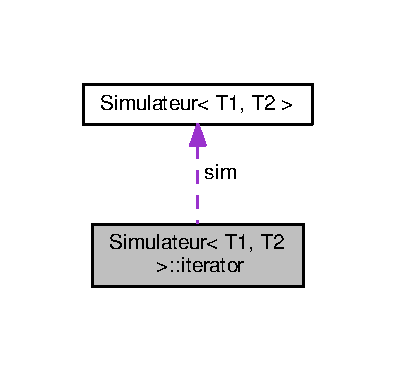
\includegraphics[width=190pt]{class_simulateur_1_1iterator__coll__graph}
\end{center}
\end{figure}
\subsection*{Fonctions membres publiques}
\begin{DoxyCompactItemize}
\item 
\hyperlink{class_simulateur_1_1iterator_a58f9a120930f75d59cc51448522b4870}{iterator} ()
\item 
\hyperlink{class_simulateur_1_1iterator}{iterator} \& \hyperlink{class_simulateur_1_1iterator_a07d32e6e5ea6ab1f8af9a23477cc8e23}{operator++} ()
\item 
T2 \& \hyperlink{class_simulateur_1_1iterator_a878896cca49dae651ef66a2197856772}{operator$\ast$} () const 
\item 
bool \hyperlink{class_simulateur_1_1iterator_ac3692e096d4fc5005eb915f46c562efe}{operator!=} (\hyperlink{class_simulateur_1_1iterator}{iterator} it) const 
\end{DoxyCompactItemize}
\subsection*{Fonctions membres privées}
\begin{DoxyCompactItemize}
\item 
\hyperlink{class_simulateur_1_1iterator_ab03c61222a97d94ec2d653e2d94912e9}{iterator} (\hyperlink{class_simulateur}{Simulateur} $\ast$s)
\item 
\hyperlink{class_simulateur_1_1iterator_acbbcdfedf00c642662752ca11032c81e}{iterator} (\hyperlink{class_simulateur}{Simulateur} $\ast$s, int dep)
\end{DoxyCompactItemize}
\subsection*{Attributs privés}
\begin{DoxyCompactItemize}
\item 
\hyperlink{class_simulateur}{Simulateur} $\ast$ \hyperlink{class_simulateur_1_1iterator_aefe7dba8b546a3b2baabe60dfbed43f8}{sim}
\item 
int \hyperlink{class_simulateur_1_1iterator_ac4a7c0f2c42b4b85f598b36674b1d772}{i}
\end{DoxyCompactItemize}
\subsection*{Amis}
\begin{DoxyCompactItemize}
\item 
class \hyperlink{class_simulateur_1_1iterator_ae6c3966e699bf920c86e0bd006bd8183}{Simulateur}
\end{DoxyCompactItemize}


\subsection{Description détaillée}
\subsubsection*{template$<$class T1, class T2$>$\\*
class Simulateur$<$ T1, T2 $>$\+::iterator}

permet le parcourt des états 

\subsection{Documentation des constructeurs et destructeur}
\index{Simulateur\+::iterator@{Simulateur\+::iterator}!iterator@{iterator}}
\index{iterator@{iterator}!Simulateur\+::iterator@{Simulateur\+::iterator}}
\subsubsection[{\texorpdfstring{iterator(\+Simulateur $\ast$s)}{iterator(Simulateur *s)}}]{\setlength{\rightskip}{0pt plus 5cm}template$<$class T1 , class T2 $>$ {\bf Simulateur}$<$ T1, T2 $>$\+::iterator\+::iterator (
\begin{DoxyParamCaption}
\item[{{\bf Simulateur} $\ast$}]{s}
\end{DoxyParamCaption}
)\hspace{0.3cm}{\ttfamily [inline]}, {\ttfamily [private]}}\hypertarget{class_simulateur_1_1iterator_ab03c61222a97d94ec2d653e2d94912e9}{}\label{class_simulateur_1_1iterator_ab03c61222a97d94ec2d653e2d94912e9}
\index{Simulateur\+::iterator@{Simulateur\+::iterator}!iterator@{iterator}}
\index{iterator@{iterator}!Simulateur\+::iterator@{Simulateur\+::iterator}}
\subsubsection[{\texorpdfstring{iterator(\+Simulateur $\ast$s, int dep)}{iterator(Simulateur *s, int dep)}}]{\setlength{\rightskip}{0pt plus 5cm}template$<$class T1 , class T2 $>$ {\bf Simulateur}$<$ T1, T2 $>$\+::iterator\+::iterator (
\begin{DoxyParamCaption}
\item[{{\bf Simulateur} $\ast$}]{s, }
\item[{int}]{dep}
\end{DoxyParamCaption}
)\hspace{0.3cm}{\ttfamily [inline]}, {\ttfamily [private]}}\hypertarget{class_simulateur_1_1iterator_acbbcdfedf00c642662752ca11032c81e}{}\label{class_simulateur_1_1iterator_acbbcdfedf00c642662752ca11032c81e}
\index{Simulateur\+::iterator@{Simulateur\+::iterator}!iterator@{iterator}}
\index{iterator@{iterator}!Simulateur\+::iterator@{Simulateur\+::iterator}}
\subsubsection[{\texorpdfstring{iterator()}{iterator()}}]{\setlength{\rightskip}{0pt plus 5cm}template$<$class T1 , class T2 $>$ {\bf Simulateur}$<$ T1, T2 $>$\+::iterator\+::iterator (
\begin{DoxyParamCaption}
{}
\end{DoxyParamCaption}
)\hspace{0.3cm}{\ttfamily [inline]}}\hypertarget{class_simulateur_1_1iterator_a58f9a120930f75d59cc51448522b4870}{}\label{class_simulateur_1_1iterator_a58f9a120930f75d59cc51448522b4870}


\subsection{Documentation des fonctions membres}
\index{Simulateur\+::iterator@{Simulateur\+::iterator}!operator"!=@{operator"!=}}
\index{operator"!=@{operator"!=}!Simulateur\+::iterator@{Simulateur\+::iterator}}
\subsubsection[{\texorpdfstring{operator"!=(iterator it) const }{operator!=(iterator it) const }}]{\setlength{\rightskip}{0pt plus 5cm}template$<$class T1 , class T2 $>$ bool {\bf Simulateur}$<$ T1, T2 $>$\+::iterator\+::operator!= (
\begin{DoxyParamCaption}
\item[{{\bf iterator}}]{it}
\end{DoxyParamCaption}
) const\hspace{0.3cm}{\ttfamily [inline]}}\hypertarget{class_simulateur_1_1iterator_ac3692e096d4fc5005eb915f46c562efe}{}\label{class_simulateur_1_1iterator_ac3692e096d4fc5005eb915f46c562efe}
\index{Simulateur\+::iterator@{Simulateur\+::iterator}!operator$\ast$@{operator$\ast$}}
\index{operator$\ast$@{operator$\ast$}!Simulateur\+::iterator@{Simulateur\+::iterator}}
\subsubsection[{\texorpdfstring{operator$\ast$() const }{operator*() const }}]{\setlength{\rightskip}{0pt plus 5cm}template$<$class T1 , class T2 $>$ T2\& {\bf Simulateur}$<$ T1, T2 $>$\+::iterator\+::operator$\ast$ (
\begin{DoxyParamCaption}
{}
\end{DoxyParamCaption}
) const\hspace{0.3cm}{\ttfamily [inline]}}\hypertarget{class_simulateur_1_1iterator_a878896cca49dae651ef66a2197856772}{}\label{class_simulateur_1_1iterator_a878896cca49dae651ef66a2197856772}
\index{Simulateur\+::iterator@{Simulateur\+::iterator}!operator++@{operator++}}
\index{operator++@{operator++}!Simulateur\+::iterator@{Simulateur\+::iterator}}
\subsubsection[{\texorpdfstring{operator++()}{operator++()}}]{\setlength{\rightskip}{0pt plus 5cm}template$<$class T1 , class T2 $>$ {\bf iterator}\& {\bf Simulateur}$<$ T1, T2 $>$\+::iterator\+::operator++ (
\begin{DoxyParamCaption}
{}
\end{DoxyParamCaption}
)\hspace{0.3cm}{\ttfamily [inline]}}\hypertarget{class_simulateur_1_1iterator_a07d32e6e5ea6ab1f8af9a23477cc8e23}{}\label{class_simulateur_1_1iterator_a07d32e6e5ea6ab1f8af9a23477cc8e23}


\subsection{Documentation des fonctions amies et associées}
\index{Simulateur\+::iterator@{Simulateur\+::iterator}!Simulateur@{Simulateur}}
\index{Simulateur@{Simulateur}!Simulateur\+::iterator@{Simulateur\+::iterator}}
\subsubsection[{\texorpdfstring{Simulateur}{Simulateur}}]{\setlength{\rightskip}{0pt plus 5cm}template$<$class T1 , class T2 $>$ friend class {\bf Simulateur}\hspace{0.3cm}{\ttfamily [friend]}}\hypertarget{class_simulateur_1_1iterator_ae6c3966e699bf920c86e0bd006bd8183}{}\label{class_simulateur_1_1iterator_ae6c3966e699bf920c86e0bd006bd8183}


\subsection{Documentation des données membres}
\index{Simulateur\+::iterator@{Simulateur\+::iterator}!i@{i}}
\index{i@{i}!Simulateur\+::iterator@{Simulateur\+::iterator}}
\subsubsection[{\texorpdfstring{i}{i}}]{\setlength{\rightskip}{0pt plus 5cm}template$<$class T1 , class T2 $>$ int {\bf Simulateur}$<$ T1, T2 $>$\+::iterator\+::i\hspace{0.3cm}{\ttfamily [private]}}\hypertarget{class_simulateur_1_1iterator_ac4a7c0f2c42b4b85f598b36674b1d772}{}\label{class_simulateur_1_1iterator_ac4a7c0f2c42b4b85f598b36674b1d772}
\index{Simulateur\+::iterator@{Simulateur\+::iterator}!sim@{sim}}
\index{sim@{sim}!Simulateur\+::iterator@{Simulateur\+::iterator}}
\subsubsection[{\texorpdfstring{sim}{sim}}]{\setlength{\rightskip}{0pt plus 5cm}template$<$class T1 , class T2 $>$ {\bf Simulateur}$\ast$ {\bf Simulateur}$<$ T1, T2 $>$\+::iterator\+::sim\hspace{0.3cm}{\ttfamily [private]}}\hypertarget{class_simulateur_1_1iterator_aefe7dba8b546a3b2baabe60dfbed43f8}{}\label{class_simulateur_1_1iterator_aefe7dba8b546a3b2baabe60dfbed43f8}


La documentation de cette classe a été générée à partir du fichier suivant \+:\begin{DoxyCompactItemize}
\item 
info/\+L\+O21/\+L\+O21/\+Auto\+Cell/\hyperlink{_simulateur_8h}{Simulateur.\+h}\end{DoxyCompactItemize}

\hypertarget{class_main_window}{}\section{Référence de la classe Main\+Window}
\label{class_main_window}\index{Main\+Window@{Main\+Window}}


hérite de Q\+Main\+Window Représente la fenêtre principal de l\textquotesingle{}application  




{\ttfamily \#include $<$mainwindow.\+h$>$}



Graphe d\textquotesingle{}héritage de Main\+Window\+:\nopagebreak
\begin{figure}[H]
\begin{center}
\leavevmode
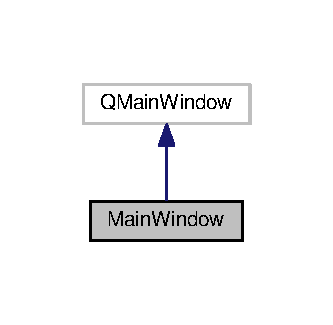
\includegraphics[width=160pt]{class_main_window__inherit__graph}
\end{center}
\end{figure}


Graphe de collaboration de Main\+Window\+:\nopagebreak
\begin{figure}[H]
\begin{center}
\leavevmode
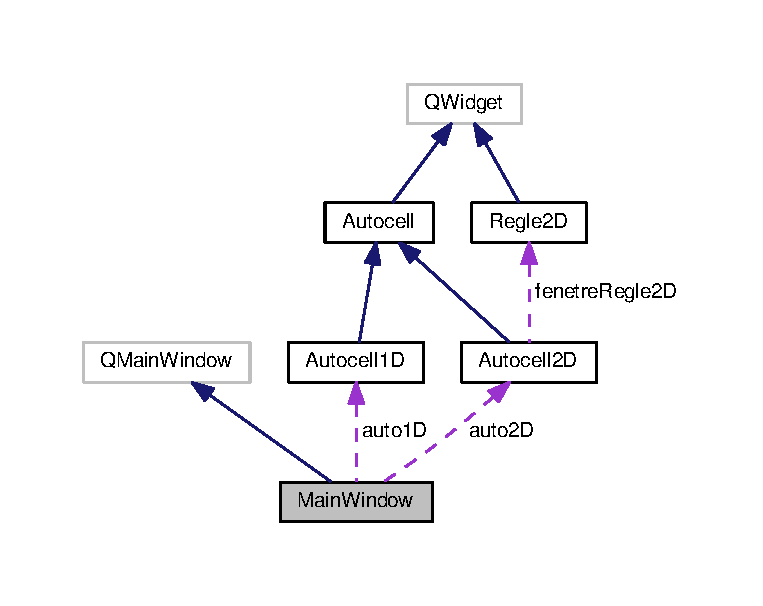
\includegraphics[width=350pt]{class_main_window__coll__graph}
\end{center}
\end{figure}
\subsection*{Connecteurs publics}
\begin{DoxyCompactItemize}
\item 
void \hyperlink{class_main_window_a13e1e518cda3c3ef508f319e5230a425}{open\+Sim} ()
\begin{DoxyCompactList}\small\item\em S\+L\+OT qui ouvre un automate choisit dans l\textquotesingle{}attribut membre choix\+Sim. \end{DoxyCompactList}\item 
void \hyperlink{class_main_window_a97b2dcddfafe0559b8b0e631f2bcf375}{clear\+Auto1D} ()
\begin{DoxyCompactList}\small\item\em S\+L\+OT qui nettoie le attribut et les options à la destruction de l\textquotesingle{}automate 1D méthode vituelle. \end{DoxyCompactList}\item 
void \hyperlink{class_main_window_a37e61e72d181b0a43900167b582caeb4}{clear\+Auto2D} ()
\begin{DoxyCompactList}\small\item\em S\+L\+OT qui nettoie le attribut à la destruction de l\textquotesingle{}automate 1D méthode vituelle. \end{DoxyCompactList}\item 
void \hyperlink{class_main_window_a709661eaabd6f570a8942f66f7c07738}{change\+Color} (Q\+String)
\begin{DoxyCompactList}\small\item\em S\+L\+OT qui gère le changement de couleur de l\textquotesingle{}automate courant. \end{DoxyCompactList}\item 
void \hyperlink{class_main_window_a06ce6c068fd97d586543f7cdd535d23a}{change\+Size} ()
\begin{DoxyCompactList}\small\item\em S\+L\+OT qui gère le changement de taille de l\textquotesingle{}automate courant. \end{DoxyCompactList}\item 
void \hyperlink{class_main_window_ac907dba426762ffbf3a7702af0aba74b}{change\+Hauteur} (int a)
\begin{DoxyCompactList}\small\item\em S\+L\+OT qui gère le changement de hauteur de l\textquotesingle{}automate courant. \end{DoxyCompactList}\item 
void \hyperlink{class_main_window_a9f316199d2ac2937364bf417cbd0aa30}{change\+Largeur} (int a)
\begin{DoxyCompactList}\small\item\em S\+L\+OT qui gère le changement de hauteur de l\textquotesingle{}automate courant. \end{DoxyCompactList}\item 
virtual void \hyperlink{class_main_window_abcab912ee0f094d4a6599b9f78f4c182}{change\+Regle1D} (int a)
\begin{DoxyCompactList}\small\item\em S\+L\+OT qui gère le changement de règle de l\textquotesingle{}automate1D. \end{DoxyCompactList}\item 
void \hyperlink{class_main_window_aae185fa2271003f1cce8d7182acae455}{change\+Speed} (int s)
\begin{DoxyCompactList}\small\item\em S\+L\+OT qui gère le changement de délai de l\textquotesingle{}automate courant. \end{DoxyCompactList}\item 
void \hyperlink{class_main_window_ab4b7fc1336fd08e311c9655edc8378c6}{change\+Taille} (int)
\begin{DoxyCompactList}\small\item\em S\+L\+OT qui gère le changement de taille de l\textquotesingle{}automate courant. \end{DoxyCompactList}\item 
virtual void \hyperlink{class_main_window_a4f035b25b6181829a9275155e3ca9bbd}{play} ()
\begin{DoxyCompactList}\small\item\em S\+L\+OT qui gère la lecture de l\textquotesingle{}automate courant. \end{DoxyCompactList}\item 
void \hyperlink{class_main_window_a17cb661f62805c510b99d9162ac8201a}{pause} ()
\begin{DoxyCompactList}\small\item\em S\+L\+OT qui gère l\textquotesingle{}arrêt de l\textquotesingle{}automate courant. \end{DoxyCompactList}\item 
void \hyperlink{class_main_window_a77557e32fb4ed3530daf2f6225c877db}{clear} ()
\begin{DoxyCompactList}\small\item\em S\+L\+OT qui gère le nettoyage de l\textquotesingle{}automate courant. \end{DoxyCompactList}\item 
virtual void \hyperlink{class_main_window_a83229b428a4774bf75bebfb6a1ae2bfe}{current} (Q\+Mdi\+Sub\+Window $\ast$w)
\begin{DoxyCompactList}\small\item\em S\+L\+OT qui gère l\textquotesingle{}affichage des options en fonction de l\textquotesingle{}automate courant. \end{DoxyCompactList}\item 
virtual void \hyperlink{class_main_window_a9a12b2903cb870b374af5f0ab8df7bda}{allow} ()
\begin{DoxyCompactList}\small\item\em S\+L\+OT qui permet d\textquotesingle{}activer le bouton pour nettoyer l\textquotesingle{}automate (quand on est en lecture on ne peut pas clear) \end{DoxyCompactList}\item 
void \hyperlink{class_main_window_ab14d52a2b2a63b6ed930e4131322dd3d}{afficher\+Regle2D} ()
\begin{DoxyCompactList}\small\item\em S\+L\+OT qui permet d\textquotesingle{}afficherla fenêtre de saisie des règles pour l\textquotesingle{}automate2D. \end{DoxyCompactList}\item 
void \hyperlink{class_main_window_a2ee1589220ee377441d94777ccef6c9f}{initialiseur} ()
\begin{DoxyCompactList}\small\item\em S\+L\+OT qui gère la génération d\textquotesingle{}un état initial aléatoire en fonction de l\textquotesingle{}automate courant. \end{DoxyCompactList}\item 
void \hyperlink{class_main_window_a611ef20ef8820089fe62ea686f321456}{initialiseur\+Sym} ()
\begin{DoxyCompactList}\small\item\em S\+L\+OT qui gère la génération d\textquotesingle{}un état initial symétrique en fonction de l\textquotesingle{}automate courant. \end{DoxyCompactList}\item 
void \hyperlink{class_main_window_a4106cf25ea9980d703e04bac7c9ecd31}{save\+Automate} ()
\begin{DoxyCompactList}\small\item\em S\+L\+OT permettant la sauvegarde d\textquotesingle{}un \hyperlink{class_automate}{Automate} 1D ou 2D. \end{DoxyCompactList}\item 
void \hyperlink{class_main_window_ad9bd4644e729ca73c06d51378aa05753}{load\+Automate} ()
\begin{DoxyCompactList}\small\item\em S\+L\+OT permettant le chargement d\textquotesingle{}un \hyperlink{class_automate}{Automate} 1D ou 2D. \end{DoxyCompactList}\end{DoxyCompactItemize}
\subsection*{Fonctions membres publiques}
\begin{DoxyCompactItemize}
\item 
\hyperlink{class_main_window_a996c5a2b6f77944776856f08ec30858d}{Main\+Window} (Q\+Widget $\ast$parent=nullptr)
\begin{DoxyCompactList}\small\item\em Constructeur. \end{DoxyCompactList}\item 
virtual void \hyperlink{class_main_window_a4e20a4a065fbb0e4d3532a45a0a91425}{close\+Event} (Q\+Close\+Event $\ast$event)
\begin{DoxyCompactList}\small\item\em méthode permettant de contrôler le comportement de l\textquotesingle{}application lors de la fermeture méthode vituelle \end{DoxyCompactList}\item 
virtual void \hyperlink{class_main_window_a94b693e3fa35f35ba200d2427b9cd419}{save\+App\+State} ()
\begin{DoxyCompactList}\small\item\em méthode permettant la sauvegarde des informations nécessaires à la réouverture en l\textquotesingle{}état de l\textquotesingle{}application méthode vituelle \end{DoxyCompactList}\item 
virtual void \hyperlink{class_main_window_a21fadb05c4f0a6686460bdd4b44896db}{extension\+Save\+App\+State} ()
\begin{DoxyCompactList}\small\item\em méthode qui permet d\textquotesingle{}ajouter des options à sauvegarder dans \hyperlink{class_main_window_a94b693e3fa35f35ba200d2427b9cd419}{save\+App\+State()} \mbox{[}Hook\mbox{]} méthode vituelle \end{DoxyCompactList}\item 
virtual void \hyperlink{class_main_window_a7c6d8bcd0b42176c57f22c166925b7d1}{extension\+Restore\+App\+State} ()
\begin{DoxyCompactList}\small\item\em méthode qui permet d\textquotesingle{}ajouter des options à sauvegarder dans \hyperlink{class_main_window_a94b693e3fa35f35ba200d2427b9cd419}{save\+App\+State()} \mbox{[}Hook\mbox{]} méthode vituelle \end{DoxyCompactList}\item 
virtual void \hyperlink{class_main_window_ab1dbe77cfb9a4876733a540614afdec0}{restore\+App\+State} ()
\begin{DoxyCompactList}\small\item\em méthode appelée avant la méthode show() de la mainwindow afin de restaurer la dernière session méthode vituelle \end{DoxyCompactList}\item 
virtual void \hyperlink{class_main_window_aec09ccd11397e7c8f83852ede698cf9c}{extension\+Open\+Sim} ()
\begin{DoxyCompactList}\small\item\em méthode qui permet d\textquotesingle{}ajouter des automates dans le S\+L\+OT \hyperlink{class_main_window_a13e1e518cda3c3ef508f319e5230a425}{open\+Sim()} \mbox{[}Hook\mbox{]} méthode vituelle \end{DoxyCompactList}\item 
virtual void \hyperlink{class_main_window_a51581d05a87d52c310c5232b4d05a2ea}{extensionclear\+Auto1D} ()
\begin{DoxyCompactList}\small\item\em méthode qui permet d\textquotesingle{}ajouter des actions lors du nettoyage des attributs dans le S\+L\+OT \hyperlink{class_main_window_a97b2dcddfafe0559b8b0e631f2bcf375}{clear\+Auto1\+D()} \mbox{[}Hook\mbox{]} méthode vituelle \end{DoxyCompactList}\item 
virtual void \hyperlink{class_main_window_a44411b6c7380592b08589b6edde6b5dc}{extensionclear\+Auto2D} ()
\begin{DoxyCompactList}\small\item\em méthode qui permet d\textquotesingle{}ajouter des actions lors du nettoyage des attributs dans le S\+L\+OT \hyperlink{class_main_window_a37e61e72d181b0a43900167b582caeb4}{clear\+Auto2\+D()} \mbox{[}Hook\mbox{]} méthode vituelle \end{DoxyCompactList}\end{DoxyCompactItemize}
\subsection*{Fonctions membres privées}
\begin{DoxyCompactItemize}
\item 
virtual void \hyperlink{class_main_window_aeb57235ebc08860e680132db167c09b4}{create\+Tool\+Bar} ()
\begin{DoxyCompactList}\small\item\em construit la barre d\textquotesingle{}outil méthode virtuelle privée utilisée dans le constructeur \end{DoxyCompactList}\item 
virtual void \hyperlink{class_main_window_a57d11300ed1f37447626810acbcfd6c4}{create\+Dock\+Option} ()
\begin{DoxyCompactList}\small\item\em construit les options méthode virtuelle privée utilisée dans le constructeur \end{DoxyCompactList}\item 
virtual void \hyperlink{class_main_window_a6de156fdb121e0c7f7b940eca3633087}{create\+Mdi\+Area} ()
\begin{DoxyCompactList}\small\item\em construit la zone centrale méthode virtuelle privée utilisée dans le constructeur \end{DoxyCompactList}\item 
virtual void \hyperlink{class_main_window_a8ab1b6ec65be939f3f3927e2fff93756}{create\+Option1D} ()
\begin{DoxyCompactList}\small\item\em construit les options pour l\textquotesingle{}automate1D méthode virtuelle privée utilisée dans le constructeur \end{DoxyCompactList}\item 
virtual void \hyperlink{class_main_window_a45eb73f1c5f7a104c6bb7d14c281435c}{create\+Option2D} ()
\begin{DoxyCompactList}\small\item\em construit les options pour l\textquotesingle{}automate2D méthode virtuelle privée utilisée dans le constructeur \end{DoxyCompactList}\end{DoxyCompactItemize}
\subsection*{Attributs privés}
\begin{DoxyCompactItemize}
\item 
Q\+Tool\+Bar $\ast$ \hyperlink{class_main_window_a10d2a8149dc4da0a7df5ee9e4e189721}{tool\+Bar}
\item 
std\+::vector$<$ Q\+Icon $\ast$ $>$ \hyperlink{class_main_window_ab903c7e6c6310d5ae1455d5935ec446a}{icon}
\item 
std\+::vector$<$ Q\+Action $\ast$ $>$ \hyperlink{class_main_window_a03fc8c2845f51b55f2b733c9ad66a0c8}{action}
\item 
std\+::vector$<$ Q\+Label $\ast$ $>$ \hyperlink{class_main_window_a4d2abb2a3dc6e601f8ed99ec58879f79}{label}
\item 
Q\+Combo\+Box $\ast$ \hyperlink{class_main_window_a11ee55d02a2bccaf673267f930bc0f90}{choix\+Sim}
\item 
Q\+Group\+Box $\ast$ \hyperlink{class_main_window_a69406bb359d08dd42c0a05957ae89b51}{box\+Dim}
\item 
Q\+Grid\+Layout $\ast$ \hyperlink{class_main_window_a1827baeeedb3477f4fd4c705aedda5c1}{layout\+Box\+Dim}
\item 
Q\+Group\+Box $\ast$ \hyperlink{class_main_window_ac7c010cdcd4cafe4a9ac0b87ad384b8a}{box\+Cel}
\item 
Q\+Grid\+Layout $\ast$ \hyperlink{class_main_window_accffbd02cf5f6e812592410d90a2bf01}{layout\+Box\+Cel}
\item 
Q\+Widget $\ast$ \hyperlink{class_main_window_a676e5f857b1b37f685cce4d1b53e221c}{option1D}
\item 
Q\+Grid\+Layout $\ast$ \hyperlink{class_main_window_a25605b8d3fa4ec4b5cef93bb266136e7}{layout1D}
\item 
Q\+Spin\+Box $\ast$ \hyperlink{class_main_window_a8ea57e6e7e57cbe0e03ebb75a385439a}{larg1D}
\item 
Q\+Spin\+Box $\ast$ \hyperlink{class_main_window_adf5c1f107d4ba21b762ddde7c9284f57}{nb\+Sim1D}
\item 
Q\+Spin\+Box $\ast$ \hyperlink{class_main_window_ad652e5a8e2bbf95af39779853bab4142}{regle1D}
\item 
Q\+Combo\+Box $\ast$ \hyperlink{class_main_window_aae0246fdb4536b62a90c2fd39fef98ab}{couleur}
\item 
Q\+Widget $\ast$ \hyperlink{class_main_window_abe71dc980ca6f6a52d5d0f9bf0902dff}{option2D}
\item 
Q\+Grid\+Layout $\ast$ \hyperlink{class_main_window_a648672720c15d3b363c131c91408422d}{layout2D}
\item 
Q\+Grid\+Layout $\ast$ \hyperlink{class_main_window_a7ab6b649b9761ce29bcda27ebbbe9ccd}{layout\+Box\+Dim2D}
\item 
Q\+Group\+Box $\ast$ \hyperlink{class_main_window_a1d591f82ca53c455c4a5204f8baad925}{box\+Cel2D}
\item 
Q\+Group\+Box $\ast$ \hyperlink{class_main_window_ad25e047b431ec6c6d244c9d4a3355582}{box\+Dim2D}
\item 
Q\+Grid\+Layout $\ast$ \hyperlink{class_main_window_a69d0a438a34120f96b7394136ee13a15}{layout\+Box\+Cel2D}
\item 
Q\+Group\+Box $\ast$ \hyperlink{class_main_window_aa758e230a66e84a946b125af5df55618}{box\+Param2D}
\item 
Q\+Combo\+Box $\ast$ \hyperlink{class_main_window_aaba4f5a028019a18aae76c21d3ffa0d5}{mode2D}
\item 
Q\+Grid\+Layout $\ast$ \hyperlink{class_main_window_af5faffe7dcb929efd6cf1a1b823c99a1}{layout\+Box\+Param2D}
\item 
Q\+Mdi\+Area $\ast$ \hyperlink{class_main_window_a9c7c0dfa79f78e05a3745962c680cd18}{central}
\item 
Q\+Mdi\+Sub\+Window $\ast$ \hyperlink{class_main_window_ac18cc180f7f4908f63ce91487bf044cd}{sub\+Win}
\item 
Q\+Mdi\+Sub\+Window $\ast$ \hyperlink{class_main_window_a9e6a20036bfb2fe795858f32b0f72282}{sub\+Win2D}
\item 
Q\+Spin\+Box $\ast$ \hyperlink{class_main_window_af66e8d082f97a24629399dec9da7aa03}{larg2D}
\item 
Q\+Spin\+Box $\ast$ \hyperlink{class_main_window_aea127325b7c01f02b7a98b17595326bb}{haut2D}
\item 
Q\+Spin\+Box $\ast$ \hyperlink{class_main_window_a062e8ba0040a577871dd29cadbade31b}{speed2D}
\item 
Q\+Spin\+Box $\ast$ \hyperlink{class_main_window_a4ee0dd35b93263abed8d50c2517632e2}{taille}
\item 
Q\+Dock\+Widget $\ast$ \hyperlink{class_main_window_a2cfa6cfbdcaba78e37d9dd17847dd620}{option\+Dock}
\end{DoxyCompactItemize}
\subsection*{Attributs privés statiques}
\begin{DoxyCompactItemize}
\item 
static \hyperlink{class_autocell1_d}{Autocell1D} $\ast$ \hyperlink{class_main_window_a252b3e10b17bf529c25b4e72be4b4332}{auto1D} = nullptr
\item 
static \hyperlink{class_autocell2_d}{Autocell2D} $\ast$ \hyperlink{class_main_window_ae1a48aa4de447712675f3aa2d7482034}{auto2D} = nullptr
\end{DoxyCompactItemize}


\subsection{Description détaillée}
hérite de Q\+Main\+Window Représente la fenêtre principal de l\textquotesingle{}application 

\subsection{Documentation des constructeurs et destructeur}
\index{Main\+Window@{Main\+Window}!Main\+Window@{Main\+Window}}
\index{Main\+Window@{Main\+Window}!Main\+Window@{Main\+Window}}
\subsubsection[{\texorpdfstring{Main\+Window(\+Q\+Widget $\ast$parent=nullptr)}{MainWindow(QWidget *parent=nullptr)}}]{\setlength{\rightskip}{0pt plus 5cm}Main\+Window\+::\+Main\+Window (
\begin{DoxyParamCaption}
\item[{Q\+Widget $\ast$}]{parent = {\ttfamily nullptr}}
\end{DoxyParamCaption}
)}\hypertarget{class_main_window_a996c5a2b6f77944776856f08ec30858d}{}\label{class_main_window_a996c5a2b6f77944776856f08ec30858d}


Constructeur. 



\subsection{Documentation des fonctions membres}
\index{Main\+Window@{Main\+Window}!afficher\+Regle2D@{afficher\+Regle2D}}
\index{afficher\+Regle2D@{afficher\+Regle2D}!Main\+Window@{Main\+Window}}
\subsubsection[{\texorpdfstring{afficher\+Regle2D}{afficherRegle2D}}]{\setlength{\rightskip}{0pt plus 5cm}void Main\+Window\+::afficher\+Regle2D (
\begin{DoxyParamCaption}
{}
\end{DoxyParamCaption}
)\hspace{0.3cm}{\ttfamily [inline]}, {\ttfamily [slot]}}\hypertarget{class_main_window_ab14d52a2b2a63b6ed930e4131322dd3d}{}\label{class_main_window_ab14d52a2b2a63b6ed930e4131322dd3d}


S\+L\+OT qui permet d\textquotesingle{}afficherla fenêtre de saisie des règles pour l\textquotesingle{}automate2D. 

\index{Main\+Window@{Main\+Window}!allow@{allow}}
\index{allow@{allow}!Main\+Window@{Main\+Window}}
\subsubsection[{\texorpdfstring{allow}{allow}}]{\setlength{\rightskip}{0pt plus 5cm}virtual void Main\+Window\+::allow (
\begin{DoxyParamCaption}
{}
\end{DoxyParamCaption}
)\hspace{0.3cm}{\ttfamily [inline]}, {\ttfamily [virtual]}, {\ttfamily [slot]}}\hypertarget{class_main_window_a9a12b2903cb870b374af5f0ab8df7bda}{}\label{class_main_window_a9a12b2903cb870b374af5f0ab8df7bda}


S\+L\+OT qui permet d\textquotesingle{}activer le bouton pour nettoyer l\textquotesingle{}automate (quand on est en lecture on ne peut pas clear) 

\index{Main\+Window@{Main\+Window}!change\+Color@{change\+Color}}
\index{change\+Color@{change\+Color}!Main\+Window@{Main\+Window}}
\subsubsection[{\texorpdfstring{change\+Color}{changeColor}}]{\setlength{\rightskip}{0pt plus 5cm}void Main\+Window\+::change\+Color (
\begin{DoxyParamCaption}
\item[{Q\+String}]{a}
\end{DoxyParamCaption}
)\hspace{0.3cm}{\ttfamily [slot]}}\hypertarget{class_main_window_a709661eaabd6f570a8942f66f7c07738}{}\label{class_main_window_a709661eaabd6f570a8942f66f7c07738}


S\+L\+OT qui gère le changement de couleur de l\textquotesingle{}automate courant. 

\index{Main\+Window@{Main\+Window}!change\+Hauteur@{change\+Hauteur}}
\index{change\+Hauteur@{change\+Hauteur}!Main\+Window@{Main\+Window}}
\subsubsection[{\texorpdfstring{change\+Hauteur}{changeHauteur}}]{\setlength{\rightskip}{0pt plus 5cm}void Main\+Window\+::change\+Hauteur (
\begin{DoxyParamCaption}
\item[{int}]{a}
\end{DoxyParamCaption}
)\hspace{0.3cm}{\ttfamily [slot]}}\hypertarget{class_main_window_ac907dba426762ffbf3a7702af0aba74b}{}\label{class_main_window_ac907dba426762ffbf3a7702af0aba74b}


S\+L\+OT qui gère le changement de hauteur de l\textquotesingle{}automate courant. 


\begin{DoxyParams}{Paramètres}
{\em a} & \+: nouvelle hauteur \+: int \\
\hline
\end{DoxyParams}
\index{Main\+Window@{Main\+Window}!change\+Largeur@{change\+Largeur}}
\index{change\+Largeur@{change\+Largeur}!Main\+Window@{Main\+Window}}
\subsubsection[{\texorpdfstring{change\+Largeur}{changeLargeur}}]{\setlength{\rightskip}{0pt plus 5cm}void Main\+Window\+::change\+Largeur (
\begin{DoxyParamCaption}
\item[{int}]{a}
\end{DoxyParamCaption}
)\hspace{0.3cm}{\ttfamily [slot]}}\hypertarget{class_main_window_a9f316199d2ac2937364bf417cbd0aa30}{}\label{class_main_window_a9f316199d2ac2937364bf417cbd0aa30}


S\+L\+OT qui gère le changement de hauteur de l\textquotesingle{}automate courant. 


\begin{DoxyParams}{Paramètres}
{\em a} & \+: nouvelle largeur \+: int \\
\hline
\end{DoxyParams}
\index{Main\+Window@{Main\+Window}!change\+Regle1D@{change\+Regle1D}}
\index{change\+Regle1D@{change\+Regle1D}!Main\+Window@{Main\+Window}}
\subsubsection[{\texorpdfstring{change\+Regle1D}{changeRegle1D}}]{\setlength{\rightskip}{0pt plus 5cm}void Main\+Window\+::change\+Regle1D (
\begin{DoxyParamCaption}
\item[{int}]{a}
\end{DoxyParamCaption}
)\hspace{0.3cm}{\ttfamily [virtual]}, {\ttfamily [slot]}}\hypertarget{class_main_window_abcab912ee0f094d4a6599b9f78f4c182}{}\label{class_main_window_abcab912ee0f094d4a6599b9f78f4c182}


S\+L\+OT qui gère le changement de règle de l\textquotesingle{}automate1D. 


\begin{DoxyParams}{Paramètres}
{\em a} & \+: nouvelle règle \+: int \\
\hline
\end{DoxyParams}
\index{Main\+Window@{Main\+Window}!change\+Size@{change\+Size}}
\index{change\+Size@{change\+Size}!Main\+Window@{Main\+Window}}
\subsubsection[{\texorpdfstring{change\+Size}{changeSize}}]{\setlength{\rightskip}{0pt plus 5cm}void Main\+Window\+::change\+Size (
\begin{DoxyParamCaption}
{}
\end{DoxyParamCaption}
)\hspace{0.3cm}{\ttfamily [slot]}}\hypertarget{class_main_window_a06ce6c068fd97d586543f7cdd535d23a}{}\label{class_main_window_a06ce6c068fd97d586543f7cdd535d23a}


S\+L\+OT qui gère le changement de taille de l\textquotesingle{}automate courant. 

\index{Main\+Window@{Main\+Window}!change\+Speed@{change\+Speed}}
\index{change\+Speed@{change\+Speed}!Main\+Window@{Main\+Window}}
\subsubsection[{\texorpdfstring{change\+Speed}{changeSpeed}}]{\setlength{\rightskip}{0pt plus 5cm}void Main\+Window\+::change\+Speed (
\begin{DoxyParamCaption}
\item[{int}]{s}
\end{DoxyParamCaption}
)\hspace{0.3cm}{\ttfamily [slot]}}\hypertarget{class_main_window_aae185fa2271003f1cce8d7182acae455}{}\label{class_main_window_aae185fa2271003f1cce8d7182acae455}


S\+L\+OT qui gère le changement de délai de l\textquotesingle{}automate courant. 


\begin{DoxyParams}{Paramètres}
{\em a} & \+: nouveau délai \+: int \\
\hline
\end{DoxyParams}
\index{Main\+Window@{Main\+Window}!change\+Taille@{change\+Taille}}
\index{change\+Taille@{change\+Taille}!Main\+Window@{Main\+Window}}
\subsubsection[{\texorpdfstring{change\+Taille}{changeTaille}}]{\setlength{\rightskip}{0pt plus 5cm}void Main\+Window\+::change\+Taille (
\begin{DoxyParamCaption}
\item[{int}]{t}
\end{DoxyParamCaption}
)\hspace{0.3cm}{\ttfamily [slot]}}\hypertarget{class_main_window_ab4b7fc1336fd08e311c9655edc8378c6}{}\label{class_main_window_ab4b7fc1336fd08e311c9655edc8378c6}


S\+L\+OT qui gère le changement de taille de l\textquotesingle{}automate courant. 


\begin{DoxyParams}{Paramètres}
{\em taille} & \+: nouvelle taille \+: int \\
\hline
\end{DoxyParams}
\index{Main\+Window@{Main\+Window}!clear@{clear}}
\index{clear@{clear}!Main\+Window@{Main\+Window}}
\subsubsection[{\texorpdfstring{clear}{clear}}]{\setlength{\rightskip}{0pt plus 5cm}void Main\+Window\+::clear (
\begin{DoxyParamCaption}
{}
\end{DoxyParamCaption}
)\hspace{0.3cm}{\ttfamily [slot]}}\hypertarget{class_main_window_a77557e32fb4ed3530daf2f6225c877db}{}\label{class_main_window_a77557e32fb4ed3530daf2f6225c877db}


S\+L\+OT qui gère le nettoyage de l\textquotesingle{}automate courant. 

\index{Main\+Window@{Main\+Window}!clear\+Auto1D@{clear\+Auto1D}}
\index{clear\+Auto1D@{clear\+Auto1D}!Main\+Window@{Main\+Window}}
\subsubsection[{\texorpdfstring{clear\+Auto1D}{clearAuto1D}}]{\setlength{\rightskip}{0pt plus 5cm}void Main\+Window\+::clear\+Auto1D (
\begin{DoxyParamCaption}
{}
\end{DoxyParamCaption}
)\hspace{0.3cm}{\ttfamily [inline]}, {\ttfamily [slot]}}\hypertarget{class_main_window_a97b2dcddfafe0559b8b0e631f2bcf375}{}\label{class_main_window_a97b2dcddfafe0559b8b0e631f2bcf375}


S\+L\+OT qui nettoie le attribut et les options à la destruction de l\textquotesingle{}automate 1D méthode vituelle. 

\index{Main\+Window@{Main\+Window}!clear\+Auto2D@{clear\+Auto2D}}
\index{clear\+Auto2D@{clear\+Auto2D}!Main\+Window@{Main\+Window}}
\subsubsection[{\texorpdfstring{clear\+Auto2D}{clearAuto2D}}]{\setlength{\rightskip}{0pt plus 5cm}void Main\+Window\+::clear\+Auto2D (
\begin{DoxyParamCaption}
{}
\end{DoxyParamCaption}
)\hspace{0.3cm}{\ttfamily [inline]}, {\ttfamily [slot]}}\hypertarget{class_main_window_a37e61e72d181b0a43900167b582caeb4}{}\label{class_main_window_a37e61e72d181b0a43900167b582caeb4}


S\+L\+OT qui nettoie le attribut à la destruction de l\textquotesingle{}automate 1D méthode vituelle. 

\index{Main\+Window@{Main\+Window}!close\+Event@{close\+Event}}
\index{close\+Event@{close\+Event}!Main\+Window@{Main\+Window}}
\subsubsection[{\texorpdfstring{close\+Event(\+Q\+Close\+Event $\ast$event)}{closeEvent(QCloseEvent *event)}}]{\setlength{\rightskip}{0pt plus 5cm}void Main\+Window\+::close\+Event (
\begin{DoxyParamCaption}
\item[{Q\+Close\+Event $\ast$}]{event}
\end{DoxyParamCaption}
)\hspace{0.3cm}{\ttfamily [virtual]}}\hypertarget{class_main_window_a4e20a4a065fbb0e4d3532a45a0a91425}{}\label{class_main_window_a4e20a4a065fbb0e4d3532a45a0a91425}


méthode permettant de contrôler le comportement de l\textquotesingle{}application lors de la fermeture méthode vituelle 

\index{Main\+Window@{Main\+Window}!create\+Dock\+Option@{create\+Dock\+Option}}
\index{create\+Dock\+Option@{create\+Dock\+Option}!Main\+Window@{Main\+Window}}
\subsubsection[{\texorpdfstring{create\+Dock\+Option()}{createDockOption()}}]{\setlength{\rightskip}{0pt plus 5cm}void Main\+Window\+::create\+Dock\+Option (
\begin{DoxyParamCaption}
{}
\end{DoxyParamCaption}
)\hspace{0.3cm}{\ttfamily [private]}, {\ttfamily [virtual]}}\hypertarget{class_main_window_a57d11300ed1f37447626810acbcfd6c4}{}\label{class_main_window_a57d11300ed1f37447626810acbcfd6c4}


construit les options méthode virtuelle privée utilisée dans le constructeur 

\index{Main\+Window@{Main\+Window}!create\+Mdi\+Area@{create\+Mdi\+Area}}
\index{create\+Mdi\+Area@{create\+Mdi\+Area}!Main\+Window@{Main\+Window}}
\subsubsection[{\texorpdfstring{create\+Mdi\+Area()}{createMdiArea()}}]{\setlength{\rightskip}{0pt plus 5cm}void Main\+Window\+::create\+Mdi\+Area (
\begin{DoxyParamCaption}
{}
\end{DoxyParamCaption}
)\hspace{0.3cm}{\ttfamily [private]}, {\ttfamily [virtual]}}\hypertarget{class_main_window_a6de156fdb121e0c7f7b940eca3633087}{}\label{class_main_window_a6de156fdb121e0c7f7b940eca3633087}


construit la zone centrale méthode virtuelle privée utilisée dans le constructeur 

\index{Main\+Window@{Main\+Window}!create\+Option1D@{create\+Option1D}}
\index{create\+Option1D@{create\+Option1D}!Main\+Window@{Main\+Window}}
\subsubsection[{\texorpdfstring{create\+Option1\+D()}{createOption1D()}}]{\setlength{\rightskip}{0pt plus 5cm}void Main\+Window\+::create\+Option1D (
\begin{DoxyParamCaption}
{}
\end{DoxyParamCaption}
)\hspace{0.3cm}{\ttfamily [private]}, {\ttfamily [virtual]}}\hypertarget{class_main_window_a8ab1b6ec65be939f3f3927e2fff93756}{}\label{class_main_window_a8ab1b6ec65be939f3f3927e2fff93756}


construit les options pour l\textquotesingle{}automate1D méthode virtuelle privée utilisée dans le constructeur 

\index{Main\+Window@{Main\+Window}!create\+Option2D@{create\+Option2D}}
\index{create\+Option2D@{create\+Option2D}!Main\+Window@{Main\+Window}}
\subsubsection[{\texorpdfstring{create\+Option2\+D()}{createOption2D()}}]{\setlength{\rightskip}{0pt plus 5cm}void Main\+Window\+::create\+Option2D (
\begin{DoxyParamCaption}
{}
\end{DoxyParamCaption}
)\hspace{0.3cm}{\ttfamily [private]}, {\ttfamily [virtual]}}\hypertarget{class_main_window_a45eb73f1c5f7a104c6bb7d14c281435c}{}\label{class_main_window_a45eb73f1c5f7a104c6bb7d14c281435c}


construit les options pour l\textquotesingle{}automate2D méthode virtuelle privée utilisée dans le constructeur 

\index{Main\+Window@{Main\+Window}!create\+Tool\+Bar@{create\+Tool\+Bar}}
\index{create\+Tool\+Bar@{create\+Tool\+Bar}!Main\+Window@{Main\+Window}}
\subsubsection[{\texorpdfstring{create\+Tool\+Bar()}{createToolBar()}}]{\setlength{\rightskip}{0pt plus 5cm}void Main\+Window\+::create\+Tool\+Bar (
\begin{DoxyParamCaption}
{}
\end{DoxyParamCaption}
)\hspace{0.3cm}{\ttfamily [private]}, {\ttfamily [virtual]}}\hypertarget{class_main_window_aeb57235ebc08860e680132db167c09b4}{}\label{class_main_window_aeb57235ebc08860e680132db167c09b4}


construit la barre d\textquotesingle{}outil méthode virtuelle privée utilisée dans le constructeur 

\index{Main\+Window@{Main\+Window}!current@{current}}
\index{current@{current}!Main\+Window@{Main\+Window}}
\subsubsection[{\texorpdfstring{current}{current}}]{\setlength{\rightskip}{0pt plus 5cm}void Main\+Window\+::current (
\begin{DoxyParamCaption}
\item[{Q\+Mdi\+Sub\+Window $\ast$}]{w}
\end{DoxyParamCaption}
)\hspace{0.3cm}{\ttfamily [virtual]}, {\ttfamily [slot]}}\hypertarget{class_main_window_a83229b428a4774bf75bebfb6a1ae2bfe}{}\label{class_main_window_a83229b428a4774bf75bebfb6a1ae2bfe}


S\+L\+OT qui gère l\textquotesingle{}affichage des options en fonction de l\textquotesingle{}automate courant. 


\begin{DoxyParams}{Paramètres}
{\em w} & \+: automate\+Courant \+: Q\+Mdi\+Sub\+Window $\ast$ \\
\hline
\end{DoxyParams}
\index{Main\+Window@{Main\+Window}!extensionclear\+Auto1D@{extensionclear\+Auto1D}}
\index{extensionclear\+Auto1D@{extensionclear\+Auto1D}!Main\+Window@{Main\+Window}}
\subsubsection[{\texorpdfstring{extensionclear\+Auto1\+D()}{extensionclearAuto1D()}}]{\setlength{\rightskip}{0pt plus 5cm}virtual void Main\+Window\+::extensionclear\+Auto1D (
\begin{DoxyParamCaption}
{}
\end{DoxyParamCaption}
)\hspace{0.3cm}{\ttfamily [inline]}, {\ttfamily [virtual]}}\hypertarget{class_main_window_a51581d05a87d52c310c5232b4d05a2ea}{}\label{class_main_window_a51581d05a87d52c310c5232b4d05a2ea}


méthode qui permet d\textquotesingle{}ajouter des actions lors du nettoyage des attributs dans le S\+L\+OT \hyperlink{class_main_window_a97b2dcddfafe0559b8b0e631f2bcf375}{clear\+Auto1\+D()} \mbox{[}Hook\mbox{]} méthode vituelle 

\index{Main\+Window@{Main\+Window}!extensionclear\+Auto2D@{extensionclear\+Auto2D}}
\index{extensionclear\+Auto2D@{extensionclear\+Auto2D}!Main\+Window@{Main\+Window}}
\subsubsection[{\texorpdfstring{extensionclear\+Auto2\+D()}{extensionclearAuto2D()}}]{\setlength{\rightskip}{0pt plus 5cm}virtual void Main\+Window\+::extensionclear\+Auto2D (
\begin{DoxyParamCaption}
{}
\end{DoxyParamCaption}
)\hspace{0.3cm}{\ttfamily [inline]}, {\ttfamily [virtual]}}\hypertarget{class_main_window_a44411b6c7380592b08589b6edde6b5dc}{}\label{class_main_window_a44411b6c7380592b08589b6edde6b5dc}


méthode qui permet d\textquotesingle{}ajouter des actions lors du nettoyage des attributs dans le S\+L\+OT \hyperlink{class_main_window_a37e61e72d181b0a43900167b582caeb4}{clear\+Auto2\+D()} \mbox{[}Hook\mbox{]} méthode vituelle 

\index{Main\+Window@{Main\+Window}!extension\+Open\+Sim@{extension\+Open\+Sim}}
\index{extension\+Open\+Sim@{extension\+Open\+Sim}!Main\+Window@{Main\+Window}}
\subsubsection[{\texorpdfstring{extension\+Open\+Sim()}{extensionOpenSim()}}]{\setlength{\rightskip}{0pt plus 5cm}virtual void Main\+Window\+::extension\+Open\+Sim (
\begin{DoxyParamCaption}
{}
\end{DoxyParamCaption}
)\hspace{0.3cm}{\ttfamily [inline]}, {\ttfamily [virtual]}}\hypertarget{class_main_window_aec09ccd11397e7c8f83852ede698cf9c}{}\label{class_main_window_aec09ccd11397e7c8f83852ede698cf9c}


méthode qui permet d\textquotesingle{}ajouter des automates dans le S\+L\+OT \hyperlink{class_main_window_a13e1e518cda3c3ef508f319e5230a425}{open\+Sim()} \mbox{[}Hook\mbox{]} méthode vituelle 

\index{Main\+Window@{Main\+Window}!extension\+Restore\+App\+State@{extension\+Restore\+App\+State}}
\index{extension\+Restore\+App\+State@{extension\+Restore\+App\+State}!Main\+Window@{Main\+Window}}
\subsubsection[{\texorpdfstring{extension\+Restore\+App\+State()}{extensionRestoreAppState()}}]{\setlength{\rightskip}{0pt plus 5cm}virtual void Main\+Window\+::extension\+Restore\+App\+State (
\begin{DoxyParamCaption}
{}
\end{DoxyParamCaption}
)\hspace{0.3cm}{\ttfamily [inline]}, {\ttfamily [virtual]}}\hypertarget{class_main_window_a7c6d8bcd0b42176c57f22c166925b7d1}{}\label{class_main_window_a7c6d8bcd0b42176c57f22c166925b7d1}


méthode qui permet d\textquotesingle{}ajouter des options à sauvegarder dans \hyperlink{class_main_window_a94b693e3fa35f35ba200d2427b9cd419}{save\+App\+State()} \mbox{[}Hook\mbox{]} méthode vituelle 

\index{Main\+Window@{Main\+Window}!extension\+Save\+App\+State@{extension\+Save\+App\+State}}
\index{extension\+Save\+App\+State@{extension\+Save\+App\+State}!Main\+Window@{Main\+Window}}
\subsubsection[{\texorpdfstring{extension\+Save\+App\+State()}{extensionSaveAppState()}}]{\setlength{\rightskip}{0pt plus 5cm}virtual void Main\+Window\+::extension\+Save\+App\+State (
\begin{DoxyParamCaption}
{}
\end{DoxyParamCaption}
)\hspace{0.3cm}{\ttfamily [inline]}, {\ttfamily [virtual]}}\hypertarget{class_main_window_a21fadb05c4f0a6686460bdd4b44896db}{}\label{class_main_window_a21fadb05c4f0a6686460bdd4b44896db}


méthode qui permet d\textquotesingle{}ajouter des options à sauvegarder dans \hyperlink{class_main_window_a94b693e3fa35f35ba200d2427b9cd419}{save\+App\+State()} \mbox{[}Hook\mbox{]} méthode vituelle 

\index{Main\+Window@{Main\+Window}!initialiseur@{initialiseur}}
\index{initialiseur@{initialiseur}!Main\+Window@{Main\+Window}}
\subsubsection[{\texorpdfstring{initialiseur}{initialiseur}}]{\setlength{\rightskip}{0pt plus 5cm}void Main\+Window\+::initialiseur (
\begin{DoxyParamCaption}
{}
\end{DoxyParamCaption}
)\hspace{0.3cm}{\ttfamily [slot]}}\hypertarget{class_main_window_a2ee1589220ee377441d94777ccef6c9f}{}\label{class_main_window_a2ee1589220ee377441d94777ccef6c9f}


S\+L\+OT qui gère la génération d\textquotesingle{}un état initial aléatoire en fonction de l\textquotesingle{}automate courant. 

\index{Main\+Window@{Main\+Window}!initialiseur\+Sym@{initialiseur\+Sym}}
\index{initialiseur\+Sym@{initialiseur\+Sym}!Main\+Window@{Main\+Window}}
\subsubsection[{\texorpdfstring{initialiseur\+Sym}{initialiseurSym}}]{\setlength{\rightskip}{0pt plus 5cm}void Main\+Window\+::initialiseur\+Sym (
\begin{DoxyParamCaption}
{}
\end{DoxyParamCaption}
)\hspace{0.3cm}{\ttfamily [slot]}}\hypertarget{class_main_window_a611ef20ef8820089fe62ea686f321456}{}\label{class_main_window_a611ef20ef8820089fe62ea686f321456}


S\+L\+OT qui gère la génération d\textquotesingle{}un état initial symétrique en fonction de l\textquotesingle{}automate courant. 

\index{Main\+Window@{Main\+Window}!load\+Automate@{load\+Automate}}
\index{load\+Automate@{load\+Automate}!Main\+Window@{Main\+Window}}
\subsubsection[{\texorpdfstring{load\+Automate}{loadAutomate}}]{\setlength{\rightskip}{0pt plus 5cm}void Main\+Window\+::load\+Automate (
\begin{DoxyParamCaption}
{}
\end{DoxyParamCaption}
)\hspace{0.3cm}{\ttfamily [slot]}}\hypertarget{class_main_window_ad9bd4644e729ca73c06d51378aa05753}{}\label{class_main_window_ad9bd4644e729ca73c06d51378aa05753}


S\+L\+OT permettant le chargement d\textquotesingle{}un \hyperlink{class_automate}{Automate} 1D ou 2D. 

\index{Main\+Window@{Main\+Window}!open\+Sim@{open\+Sim}}
\index{open\+Sim@{open\+Sim}!Main\+Window@{Main\+Window}}
\subsubsection[{\texorpdfstring{open\+Sim}{openSim}}]{\setlength{\rightskip}{0pt plus 5cm}void Main\+Window\+::open\+Sim (
\begin{DoxyParamCaption}
{}
\end{DoxyParamCaption}
)\hspace{0.3cm}{\ttfamily [slot]}}\hypertarget{class_main_window_a13e1e518cda3c3ef508f319e5230a425}{}\label{class_main_window_a13e1e518cda3c3ef508f319e5230a425}


S\+L\+OT qui ouvre un automate choisit dans l\textquotesingle{}attribut membre choix\+Sim. 

\index{Main\+Window@{Main\+Window}!pause@{pause}}
\index{pause@{pause}!Main\+Window@{Main\+Window}}
\subsubsection[{\texorpdfstring{pause}{pause}}]{\setlength{\rightskip}{0pt plus 5cm}void Main\+Window\+::pause (
\begin{DoxyParamCaption}
{}
\end{DoxyParamCaption}
)\hspace{0.3cm}{\ttfamily [slot]}}\hypertarget{class_main_window_a17cb661f62805c510b99d9162ac8201a}{}\label{class_main_window_a17cb661f62805c510b99d9162ac8201a}


S\+L\+OT qui gère l\textquotesingle{}arrêt de l\textquotesingle{}automate courant. 

\index{Main\+Window@{Main\+Window}!play@{play}}
\index{play@{play}!Main\+Window@{Main\+Window}}
\subsubsection[{\texorpdfstring{play}{play}}]{\setlength{\rightskip}{0pt plus 5cm}void Main\+Window\+::play (
\begin{DoxyParamCaption}
{}
\end{DoxyParamCaption}
)\hspace{0.3cm}{\ttfamily [virtual]}, {\ttfamily [slot]}}\hypertarget{class_main_window_a4f035b25b6181829a9275155e3ca9bbd}{}\label{class_main_window_a4f035b25b6181829a9275155e3ca9bbd}


S\+L\+OT qui gère la lecture de l\textquotesingle{}automate courant. 

\index{Main\+Window@{Main\+Window}!restore\+App\+State@{restore\+App\+State}}
\index{restore\+App\+State@{restore\+App\+State}!Main\+Window@{Main\+Window}}
\subsubsection[{\texorpdfstring{restore\+App\+State()}{restoreAppState()}}]{\setlength{\rightskip}{0pt plus 5cm}void Main\+Window\+::restore\+App\+State (
\begin{DoxyParamCaption}
{}
\end{DoxyParamCaption}
)\hspace{0.3cm}{\ttfamily [virtual]}}\hypertarget{class_main_window_ab1dbe77cfb9a4876733a540614afdec0}{}\label{class_main_window_ab1dbe77cfb9a4876733a540614afdec0}


méthode appelée avant la méthode show() de la mainwindow afin de restaurer la dernière session méthode vituelle 

\index{Main\+Window@{Main\+Window}!save\+App\+State@{save\+App\+State}}
\index{save\+App\+State@{save\+App\+State}!Main\+Window@{Main\+Window}}
\subsubsection[{\texorpdfstring{save\+App\+State()}{saveAppState()}}]{\setlength{\rightskip}{0pt plus 5cm}void Main\+Window\+::save\+App\+State (
\begin{DoxyParamCaption}
{}
\end{DoxyParamCaption}
)\hspace{0.3cm}{\ttfamily [virtual]}}\hypertarget{class_main_window_a94b693e3fa35f35ba200d2427b9cd419}{}\label{class_main_window_a94b693e3fa35f35ba200d2427b9cd419}


méthode permettant la sauvegarde des informations nécessaires à la réouverture en l\textquotesingle{}état de l\textquotesingle{}application méthode vituelle 

\index{Main\+Window@{Main\+Window}!save\+Automate@{save\+Automate}}
\index{save\+Automate@{save\+Automate}!Main\+Window@{Main\+Window}}
\subsubsection[{\texorpdfstring{save\+Automate}{saveAutomate}}]{\setlength{\rightskip}{0pt plus 5cm}void Main\+Window\+::save\+Automate (
\begin{DoxyParamCaption}
{}
\end{DoxyParamCaption}
)\hspace{0.3cm}{\ttfamily [slot]}}\hypertarget{class_main_window_a4106cf25ea9980d703e04bac7c9ecd31}{}\label{class_main_window_a4106cf25ea9980d703e04bac7c9ecd31}


S\+L\+OT permettant la sauvegarde d\textquotesingle{}un \hyperlink{class_automate}{Automate} 1D ou 2D. 



\subsection{Documentation des données membres}
\index{Main\+Window@{Main\+Window}!action@{action}}
\index{action@{action}!Main\+Window@{Main\+Window}}
\subsubsection[{\texorpdfstring{action}{action}}]{\setlength{\rightskip}{0pt plus 5cm}std\+::vector$<$Q\+Action $\ast$$>$ Main\+Window\+::action\hspace{0.3cm}{\ttfamily [private]}}\hypertarget{class_main_window_a03fc8c2845f51b55f2b733c9ad66a0c8}{}\label{class_main_window_a03fc8c2845f51b55f2b733c9ad66a0c8}
action de la barre d\textquotesingle{}outil \index{Main\+Window@{Main\+Window}!auto1D@{auto1D}}
\index{auto1D@{auto1D}!Main\+Window@{Main\+Window}}
\subsubsection[{\texorpdfstring{auto1D}{auto1D}}]{\setlength{\rightskip}{0pt plus 5cm}{\bf Autocell1D} $\ast$ Main\+Window\+::auto1D = nullptr\hspace{0.3cm}{\ttfamily [static]}, {\ttfamily [private]}}\hypertarget{class_main_window_a252b3e10b17bf529c25b4e72be4b4332}{}\label{class_main_window_a252b3e10b17bf529c25b4e72be4b4332}
attribut static pour l\textquotesingle{}automate 1D (on peut en construire qu\textquotesingle{}un) \index{Main\+Window@{Main\+Window}!auto2D@{auto2D}}
\index{auto2D@{auto2D}!Main\+Window@{Main\+Window}}
\subsubsection[{\texorpdfstring{auto2D}{auto2D}}]{\setlength{\rightskip}{0pt plus 5cm}{\bf Autocell2D} $\ast$ Main\+Window\+::auto2D = nullptr\hspace{0.3cm}{\ttfamily [static]}, {\ttfamily [private]}}\hypertarget{class_main_window_ae1a48aa4de447712675f3aa2d7482034}{}\label{class_main_window_ae1a48aa4de447712675f3aa2d7482034}
attribut static pour l\textquotesingle{}automate 2D (on peut en construire qu\textquotesingle{}un) \index{Main\+Window@{Main\+Window}!box\+Cel@{box\+Cel}}
\index{box\+Cel@{box\+Cel}!Main\+Window@{Main\+Window}}
\subsubsection[{\texorpdfstring{box\+Cel}{boxCel}}]{\setlength{\rightskip}{0pt plus 5cm}Q\+Group\+Box$\ast$ Main\+Window\+::box\+Cel\hspace{0.3cm}{\ttfamily [private]}}\hypertarget{class_main_window_ac7c010cdcd4cafe4a9ac0b87ad384b8a}{}\label{class_main_window_ac7c010cdcd4cafe4a9ac0b87ad384b8a}
sous option cellule \index{Main\+Window@{Main\+Window}!box\+Cel2D@{box\+Cel2D}}
\index{box\+Cel2D@{box\+Cel2D}!Main\+Window@{Main\+Window}}
\subsubsection[{\texorpdfstring{box\+Cel2D}{boxCel2D}}]{\setlength{\rightskip}{0pt plus 5cm}Q\+Group\+Box$\ast$ Main\+Window\+::box\+Cel2D\hspace{0.3cm}{\ttfamily [private]}}\hypertarget{class_main_window_a1d591f82ca53c455c4a5204f8baad925}{}\label{class_main_window_a1d591f82ca53c455c4a5204f8baad925}
sous option Cellule \index{Main\+Window@{Main\+Window}!box\+Dim@{box\+Dim}}
\index{box\+Dim@{box\+Dim}!Main\+Window@{Main\+Window}}
\subsubsection[{\texorpdfstring{box\+Dim}{boxDim}}]{\setlength{\rightskip}{0pt plus 5cm}Q\+Group\+Box$\ast$ Main\+Window\+::box\+Dim\hspace{0.3cm}{\ttfamily [private]}}\hypertarget{class_main_window_a69406bb359d08dd42c0a05957ae89b51}{}\label{class_main_window_a69406bb359d08dd42c0a05957ae89b51}
sous option dimension \index{Main\+Window@{Main\+Window}!box\+Dim2D@{box\+Dim2D}}
\index{box\+Dim2D@{box\+Dim2D}!Main\+Window@{Main\+Window}}
\subsubsection[{\texorpdfstring{box\+Dim2D}{boxDim2D}}]{\setlength{\rightskip}{0pt plus 5cm}Q\+Group\+Box$\ast$ Main\+Window\+::box\+Dim2D\hspace{0.3cm}{\ttfamily [private]}}\hypertarget{class_main_window_ad25e047b431ec6c6d244c9d4a3355582}{}\label{class_main_window_ad25e047b431ec6c6d244c9d4a3355582}
sous option dimension \index{Main\+Window@{Main\+Window}!box\+Param2D@{box\+Param2D}}
\index{box\+Param2D@{box\+Param2D}!Main\+Window@{Main\+Window}}
\subsubsection[{\texorpdfstring{box\+Param2D}{boxParam2D}}]{\setlength{\rightskip}{0pt plus 5cm}Q\+Group\+Box$\ast$ Main\+Window\+::box\+Param2D\hspace{0.3cm}{\ttfamily [private]}}\hypertarget{class_main_window_aa758e230a66e84a946b125af5df55618}{}\label{class_main_window_aa758e230a66e84a946b125af5df55618}
sous option paramètre \index{Main\+Window@{Main\+Window}!central@{central}}
\index{central@{central}!Main\+Window@{Main\+Window}}
\subsubsection[{\texorpdfstring{central}{central}}]{\setlength{\rightskip}{0pt plus 5cm}Q\+Mdi\+Area$\ast$ Main\+Window\+::central\hspace{0.3cm}{\ttfamily [private]}}\hypertarget{class_main_window_a9c7c0dfa79f78e05a3745962c680cd18}{}\label{class_main_window_a9c7c0dfa79f78e05a3745962c680cd18}
représente la zone centrale de l\textquotesingle{}application ou seront chargé les automates \index{Main\+Window@{Main\+Window}!choix\+Sim@{choix\+Sim}}
\index{choix\+Sim@{choix\+Sim}!Main\+Window@{Main\+Window}}
\subsubsection[{\texorpdfstring{choix\+Sim}{choixSim}}]{\setlength{\rightskip}{0pt plus 5cm}Q\+Combo\+Box$\ast$ Main\+Window\+::choix\+Sim\hspace{0.3cm}{\ttfamily [private]}}\hypertarget{class_main_window_a11ee55d02a2bccaf673267f930bc0f90}{}\label{class_main_window_a11ee55d02a2bccaf673267f930bc0f90}
Permet le choix de l\textquotesingle{}automate qu\textquotesingle{}on veut lancer \index{Main\+Window@{Main\+Window}!couleur@{couleur}}
\index{couleur@{couleur}!Main\+Window@{Main\+Window}}
\subsubsection[{\texorpdfstring{couleur}{couleur}}]{\setlength{\rightskip}{0pt plus 5cm}Q\+Combo\+Box$\ast$ Main\+Window\+::couleur\hspace{0.3cm}{\ttfamily [private]}}\hypertarget{class_main_window_aae0246fdb4536b62a90c2fd39fef98ab}{}\label{class_main_window_aae0246fdb4536b62a90c2fd39fef98ab}
Couleur des cellules 1D \index{Main\+Window@{Main\+Window}!haut2D@{haut2D}}
\index{haut2D@{haut2D}!Main\+Window@{Main\+Window}}
\subsubsection[{\texorpdfstring{haut2D}{haut2D}}]{\setlength{\rightskip}{0pt plus 5cm}Q\+Spin\+Box$\ast$ Main\+Window\+::haut2D\hspace{0.3cm}{\ttfamily [private]}}\hypertarget{class_main_window_aea127325b7c01f02b7a98b17595326bb}{}\label{class_main_window_aea127325b7c01f02b7a98b17595326bb}
Hauteur \index{Main\+Window@{Main\+Window}!icon@{icon}}
\index{icon@{icon}!Main\+Window@{Main\+Window}}
\subsubsection[{\texorpdfstring{icon}{icon}}]{\setlength{\rightskip}{0pt plus 5cm}std\+::vector$<$Q\+Icon $\ast$$>$ Main\+Window\+::icon\hspace{0.3cm}{\ttfamily [private]}}\hypertarget{class_main_window_ab903c7e6c6310d5ae1455d5935ec446a}{}\label{class_main_window_ab903c7e6c6310d5ae1455d5935ec446a}
icone de la barre d\textquotesingle{}outil \index{Main\+Window@{Main\+Window}!label@{label}}
\index{label@{label}!Main\+Window@{Main\+Window}}
\subsubsection[{\texorpdfstring{label}{label}}]{\setlength{\rightskip}{0pt plus 5cm}std\+::vector$<$Q\+Label $\ast$$>$ Main\+Window\+::label\hspace{0.3cm}{\ttfamily [private]}}\hypertarget{class_main_window_a4d2abb2a3dc6e601f8ed99ec58879f79}{}\label{class_main_window_a4d2abb2a3dc6e601f8ed99ec58879f79}
text de la barre d\textquotesingle{}outil \index{Main\+Window@{Main\+Window}!larg1D@{larg1D}}
\index{larg1D@{larg1D}!Main\+Window@{Main\+Window}}
\subsubsection[{\texorpdfstring{larg1D}{larg1D}}]{\setlength{\rightskip}{0pt plus 5cm}Q\+Spin\+Box$\ast$ Main\+Window\+::larg1D\hspace{0.3cm}{\ttfamily [private]}}\hypertarget{class_main_window_a8ea57e6e7e57cbe0e03ebb75a385439a}{}\label{class_main_window_a8ea57e6e7e57cbe0e03ebb75a385439a}
sous option dimension \index{Main\+Window@{Main\+Window}!larg2D@{larg2D}}
\index{larg2D@{larg2D}!Main\+Window@{Main\+Window}}
\subsubsection[{\texorpdfstring{larg2D}{larg2D}}]{\setlength{\rightskip}{0pt plus 5cm}Q\+Spin\+Box$\ast$ Main\+Window\+::larg2D\hspace{0.3cm}{\ttfamily [private]}}\hypertarget{class_main_window_af66e8d082f97a24629399dec9da7aa03}{}\label{class_main_window_af66e8d082f97a24629399dec9da7aa03}
Largeur \index{Main\+Window@{Main\+Window}!layout1D@{layout1D}}
\index{layout1D@{layout1D}!Main\+Window@{Main\+Window}}
\subsubsection[{\texorpdfstring{layout1D}{layout1D}}]{\setlength{\rightskip}{0pt plus 5cm}Q\+Grid\+Layout$\ast$ Main\+Window\+::layout1D\hspace{0.3cm}{\ttfamily [private]}}\hypertarget{class_main_window_a25605b8d3fa4ec4b5cef93bb266136e7}{}\label{class_main_window_a25605b8d3fa4ec4b5cef93bb266136e7}
layout principal des options 1D \index{Main\+Window@{Main\+Window}!layout2D@{layout2D}}
\index{layout2D@{layout2D}!Main\+Window@{Main\+Window}}
\subsubsection[{\texorpdfstring{layout2D}{layout2D}}]{\setlength{\rightskip}{0pt plus 5cm}Q\+Grid\+Layout$\ast$ Main\+Window\+::layout2D\hspace{0.3cm}{\ttfamily [private]}}\hypertarget{class_main_window_a648672720c15d3b363c131c91408422d}{}\label{class_main_window_a648672720c15d3b363c131c91408422d}
layout principal des options 1D \index{Main\+Window@{Main\+Window}!layout\+Box\+Cel@{layout\+Box\+Cel}}
\index{layout\+Box\+Cel@{layout\+Box\+Cel}!Main\+Window@{Main\+Window}}
\subsubsection[{\texorpdfstring{layout\+Box\+Cel}{layoutBoxCel}}]{\setlength{\rightskip}{0pt plus 5cm}Q\+Grid\+Layout$\ast$ Main\+Window\+::layout\+Box\+Cel\hspace{0.3cm}{\ttfamily [private]}}\hypertarget{class_main_window_accffbd02cf5f6e812592410d90a2bf01}{}\label{class_main_window_accffbd02cf5f6e812592410d90a2bf01}
layout des sous option cellule \index{Main\+Window@{Main\+Window}!layout\+Box\+Cel2D@{layout\+Box\+Cel2D}}
\index{layout\+Box\+Cel2D@{layout\+Box\+Cel2D}!Main\+Window@{Main\+Window}}
\subsubsection[{\texorpdfstring{layout\+Box\+Cel2D}{layoutBoxCel2D}}]{\setlength{\rightskip}{0pt plus 5cm}Q\+Grid\+Layout$\ast$ Main\+Window\+::layout\+Box\+Cel2D\hspace{0.3cm}{\ttfamily [private]}}\hypertarget{class_main_window_a69d0a438a34120f96b7394136ee13a15}{}\label{class_main_window_a69d0a438a34120f96b7394136ee13a15}
layout des sous option cellule 2D \index{Main\+Window@{Main\+Window}!layout\+Box\+Dim@{layout\+Box\+Dim}}
\index{layout\+Box\+Dim@{layout\+Box\+Dim}!Main\+Window@{Main\+Window}}
\subsubsection[{\texorpdfstring{layout\+Box\+Dim}{layoutBoxDim}}]{\setlength{\rightskip}{0pt plus 5cm}Q\+Grid\+Layout$\ast$ Main\+Window\+::layout\+Box\+Dim\hspace{0.3cm}{\ttfamily [private]}}\hypertarget{class_main_window_a1827baeeedb3477f4fd4c705aedda5c1}{}\label{class_main_window_a1827baeeedb3477f4fd4c705aedda5c1}
layout des sous option dimension \index{Main\+Window@{Main\+Window}!layout\+Box\+Dim2D@{layout\+Box\+Dim2D}}
\index{layout\+Box\+Dim2D@{layout\+Box\+Dim2D}!Main\+Window@{Main\+Window}}
\subsubsection[{\texorpdfstring{layout\+Box\+Dim2D}{layoutBoxDim2D}}]{\setlength{\rightskip}{0pt plus 5cm}Q\+Grid\+Layout$\ast$ Main\+Window\+::layout\+Box\+Dim2D\hspace{0.3cm}{\ttfamily [private]}}\hypertarget{class_main_window_a7ab6b649b9761ce29bcda27ebbbe9ccd}{}\label{class_main_window_a7ab6b649b9761ce29bcda27ebbbe9ccd}
layout des sous option dimension 2D \index{Main\+Window@{Main\+Window}!layout\+Box\+Param2D@{layout\+Box\+Param2D}}
\index{layout\+Box\+Param2D@{layout\+Box\+Param2D}!Main\+Window@{Main\+Window}}
\subsubsection[{\texorpdfstring{layout\+Box\+Param2D}{layoutBoxParam2D}}]{\setlength{\rightskip}{0pt plus 5cm}Q\+Grid\+Layout$\ast$ Main\+Window\+::layout\+Box\+Param2D\hspace{0.3cm}{\ttfamily [private]}}\hypertarget{class_main_window_af5faffe7dcb929efd6cf1a1b823c99a1}{}\label{class_main_window_af5faffe7dcb929efd6cf1a1b823c99a1}
layout des sous option paramètre 2D \index{Main\+Window@{Main\+Window}!mode2D@{mode2D}}
\index{mode2D@{mode2D}!Main\+Window@{Main\+Window}}
\subsubsection[{\texorpdfstring{mode2D}{mode2D}}]{\setlength{\rightskip}{0pt plus 5cm}Q\+Combo\+Box$\ast$ Main\+Window\+::mode2D\hspace{0.3cm}{\ttfamily [private]}}\hypertarget{class_main_window_aaba4f5a028019a18aae76c21d3ffa0d5}{}\label{class_main_window_aaba4f5a028019a18aae76c21d3ffa0d5}
mode de lecture 2D \index{Main\+Window@{Main\+Window}!nb\+Sim1D@{nb\+Sim1D}}
\index{nb\+Sim1D@{nb\+Sim1D}!Main\+Window@{Main\+Window}}
\subsubsection[{\texorpdfstring{nb\+Sim1D}{nbSim1D}}]{\setlength{\rightskip}{0pt plus 5cm}Q\+Spin\+Box$\ast$ Main\+Window\+::nb\+Sim1D\hspace{0.3cm}{\ttfamily [private]}}\hypertarget{class_main_window_adf5c1f107d4ba21b762ddde7c9284f57}{}\label{class_main_window_adf5c1f107d4ba21b762ddde7c9284f57}
Nombre de simulation \index{Main\+Window@{Main\+Window}!option1D@{option1D}}
\index{option1D@{option1D}!Main\+Window@{Main\+Window}}
\subsubsection[{\texorpdfstring{option1D}{option1D}}]{\setlength{\rightskip}{0pt plus 5cm}Q\+Widget$\ast$ Main\+Window\+::option1D\hspace{0.3cm}{\ttfamily [private]}}\hypertarget{class_main_window_a676e5f857b1b37f685cce4d1b53e221c}{}\label{class_main_window_a676e5f857b1b37f685cce4d1b53e221c}
représente les options de l\textquotesingle{}automate1D \index{Main\+Window@{Main\+Window}!option2D@{option2D}}
\index{option2D@{option2D}!Main\+Window@{Main\+Window}}
\subsubsection[{\texorpdfstring{option2D}{option2D}}]{\setlength{\rightskip}{0pt plus 5cm}Q\+Widget$\ast$ Main\+Window\+::option2D\hspace{0.3cm}{\ttfamily [private]}}\hypertarget{class_main_window_abe71dc980ca6f6a52d5d0f9bf0902dff}{}\label{class_main_window_abe71dc980ca6f6a52d5d0f9bf0902dff}
représente les options de l\textquotesingle{}automate2D \index{Main\+Window@{Main\+Window}!option\+Dock@{option\+Dock}}
\index{option\+Dock@{option\+Dock}!Main\+Window@{Main\+Window}}
\subsubsection[{\texorpdfstring{option\+Dock}{optionDock}}]{\setlength{\rightskip}{0pt plus 5cm}Q\+Dock\+Widget$\ast$ Main\+Window\+::option\+Dock\hspace{0.3cm}{\ttfamily [private]}}\hypertarget{class_main_window_a2cfa6cfbdcaba78e37d9dd17847dd620}{}\label{class_main_window_a2cfa6cfbdcaba78e37d9dd17847dd620}
option \index{Main\+Window@{Main\+Window}!regle1D@{regle1D}}
\index{regle1D@{regle1D}!Main\+Window@{Main\+Window}}
\subsubsection[{\texorpdfstring{regle1D}{regle1D}}]{\setlength{\rightskip}{0pt plus 5cm}Q\+Spin\+Box$\ast$ Main\+Window\+::regle1D\hspace{0.3cm}{\ttfamily [private]}}\hypertarget{class_main_window_ad652e5a8e2bbf95af39779853bab4142}{}\label{class_main_window_ad652e5a8e2bbf95af39779853bab4142}
Numéro de la règle de transition \index{Main\+Window@{Main\+Window}!speed2D@{speed2D}}
\index{speed2D@{speed2D}!Main\+Window@{Main\+Window}}
\subsubsection[{\texorpdfstring{speed2D}{speed2D}}]{\setlength{\rightskip}{0pt plus 5cm}Q\+Spin\+Box$\ast$ Main\+Window\+::speed2D\hspace{0.3cm}{\ttfamily [private]}}\hypertarget{class_main_window_a062e8ba0040a577871dd29cadbade31b}{}\label{class_main_window_a062e8ba0040a577871dd29cadbade31b}
Delai entre chaque simulation \index{Main\+Window@{Main\+Window}!sub\+Win@{sub\+Win}}
\index{sub\+Win@{sub\+Win}!Main\+Window@{Main\+Window}}
\subsubsection[{\texorpdfstring{sub\+Win}{subWin}}]{\setlength{\rightskip}{0pt plus 5cm}Q\+Mdi\+Sub\+Window$\ast$ Main\+Window\+::sub\+Win\hspace{0.3cm}{\ttfamily [private]}}\hypertarget{class_main_window_ac18cc180f7f4908f63ce91487bf044cd}{}\label{class_main_window_ac18cc180f7f4908f63ce91487bf044cd}
représente la la sub\+Window de l\textquotesingle{}automate 1D \index{Main\+Window@{Main\+Window}!sub\+Win2D@{sub\+Win2D}}
\index{sub\+Win2D@{sub\+Win2D}!Main\+Window@{Main\+Window}}
\subsubsection[{\texorpdfstring{sub\+Win2D}{subWin2D}}]{\setlength{\rightskip}{0pt plus 5cm}Q\+Mdi\+Sub\+Window$\ast$ Main\+Window\+::sub\+Win2D\hspace{0.3cm}{\ttfamily [private]}}\hypertarget{class_main_window_a9e6a20036bfb2fe795858f32b0f72282}{}\label{class_main_window_a9e6a20036bfb2fe795858f32b0f72282}
représente la la sub\+Window de l\textquotesingle{}automate 2D \index{Main\+Window@{Main\+Window}!taille@{taille}}
\index{taille@{taille}!Main\+Window@{Main\+Window}}
\subsubsection[{\texorpdfstring{taille}{taille}}]{\setlength{\rightskip}{0pt plus 5cm}Q\+Spin\+Box$\ast$ Main\+Window\+::taille\hspace{0.3cm}{\ttfamily [private]}}\hypertarget{class_main_window_a4ee0dd35b93263abed8d50c2517632e2}{}\label{class_main_window_a4ee0dd35b93263abed8d50c2517632e2}
taille des cellules \index{Main\+Window@{Main\+Window}!tool\+Bar@{tool\+Bar}}
\index{tool\+Bar@{tool\+Bar}!Main\+Window@{Main\+Window}}
\subsubsection[{\texorpdfstring{tool\+Bar}{toolBar}}]{\setlength{\rightskip}{0pt plus 5cm}Q\+Tool\+Bar$\ast$ Main\+Window\+::tool\+Bar\hspace{0.3cm}{\ttfamily [private]}}\hypertarget{class_main_window_a10d2a8149dc4da0a7df5ee9e4e189721}{}\label{class_main_window_a10d2a8149dc4da0a7df5ee9e4e189721}
barre d\textquotesingle{}outil 

La documentation de cette classe a été générée à partir des fichiers suivants \+:\begin{DoxyCompactItemize}
\item 
/home/thomaspaita/\+Bureau/info/\+L\+O21/\+L\+O21/\+Auto\+Cell/\hyperlink{mainwindow_8h}{mainwindow.\+h}\item 
/home/thomaspaita/\+Bureau/info/\+L\+O21/\+L\+O21/\+Auto\+Cell/\hyperlink{mainwindow_8cpp}{mainwindow.\+cpp}\end{DoxyCompactItemize}

\hypertarget{structqt__meta__stringdata___autocell1_d__t}{}\section{Référence de la structure qt\+\_\+meta\+\_\+stringdata\+\_\+\+Autocell1\+D\+\_\+t}
\label{structqt__meta__stringdata___autocell1_d__t}\index{qt\+\_\+meta\+\_\+stringdata\+\_\+\+Autocell1\+D\+\_\+t@{qt\+\_\+meta\+\_\+stringdata\+\_\+\+Autocell1\+D\+\_\+t}}
\subsection*{Attributs publics}
\begin{DoxyCompactItemize}
\item 
Q\+Byte\+Array\+Data \hyperlink{structqt__meta__stringdata___autocell1_d__t_ad3d50b47a705a24ada7c255ddd8c526b}{data} \mbox{[}5\mbox{]}
\item 
char \hyperlink{structqt__meta__stringdata___autocell1_d__t_aa63fa3b230b4bd59751df0a366afe39f}{stringdata0} \mbox{[}29\mbox{]}
\end{DoxyCompactItemize}


\subsection{Documentation des données membres}
\index{qt\+\_\+meta\+\_\+stringdata\+\_\+\+Autocell1\+D\+\_\+t@{qt\+\_\+meta\+\_\+stringdata\+\_\+\+Autocell1\+D\+\_\+t}!data@{data}}
\index{data@{data}!qt\+\_\+meta\+\_\+stringdata\+\_\+\+Autocell1\+D\+\_\+t@{qt\+\_\+meta\+\_\+stringdata\+\_\+\+Autocell1\+D\+\_\+t}}
\subsubsection[{\texorpdfstring{data}{data}}]{\setlength{\rightskip}{0pt plus 5cm}Q\+Byte\+Array\+Data qt\+\_\+meta\+\_\+stringdata\+\_\+\+Autocell1\+D\+\_\+t\+::data\mbox{[}5\mbox{]}}\hypertarget{structqt__meta__stringdata___autocell1_d__t_ad3d50b47a705a24ada7c255ddd8c526b}{}\label{structqt__meta__stringdata___autocell1_d__t_ad3d50b47a705a24ada7c255ddd8c526b}
\index{qt\+\_\+meta\+\_\+stringdata\+\_\+\+Autocell1\+D\+\_\+t@{qt\+\_\+meta\+\_\+stringdata\+\_\+\+Autocell1\+D\+\_\+t}!stringdata0@{stringdata0}}
\index{stringdata0@{stringdata0}!qt\+\_\+meta\+\_\+stringdata\+\_\+\+Autocell1\+D\+\_\+t@{qt\+\_\+meta\+\_\+stringdata\+\_\+\+Autocell1\+D\+\_\+t}}
\subsubsection[{\texorpdfstring{stringdata0}{stringdata0}}]{\setlength{\rightskip}{0pt plus 5cm}char qt\+\_\+meta\+\_\+stringdata\+\_\+\+Autocell1\+D\+\_\+t\+::stringdata0\mbox{[}29\mbox{]}}\hypertarget{structqt__meta__stringdata___autocell1_d__t_aa63fa3b230b4bd59751df0a366afe39f}{}\label{structqt__meta__stringdata___autocell1_d__t_aa63fa3b230b4bd59751df0a366afe39f}


La documentation de cette structure a été générée à partir du fichier suivant \+:\begin{DoxyCompactItemize}
\item 
/home/thomaspaita/\+Bureau/info/\+L\+O21/\+L\+O21/build-\/\+Auto\+Cell-\/\+Desktop-\/\+Debug/\hyperlink{moc__autocell_8cpp}{moc\+\_\+autocell.\+cpp}\end{DoxyCompactItemize}

\hypertarget{structqt__meta__stringdata___autocell2_d__t}{}\section{Référence de la structure qt\+\_\+meta\+\_\+stringdata\+\_\+\+Autocell2\+D\+\_\+t}
\label{structqt__meta__stringdata___autocell2_d__t}\index{qt\+\_\+meta\+\_\+stringdata\+\_\+\+Autocell2\+D\+\_\+t@{qt\+\_\+meta\+\_\+stringdata\+\_\+\+Autocell2\+D\+\_\+t}}
\subsection*{Attributs publics}
\begin{DoxyCompactItemize}
\item 
Q\+Byte\+Array\+Data \hyperlink{structqt__meta__stringdata___autocell2_d__t_a638a1507442e609739b5de7f12377002}{data} \mbox{[}12\mbox{]}
\item 
char \hyperlink{structqt__meta__stringdata___autocell2_d__t_abb1f63b6d95e8f7dfa1925caf0601041}{stringdata0} \mbox{[}129\mbox{]}
\end{DoxyCompactItemize}


\subsection{Documentation des données membres}
\index{qt\+\_\+meta\+\_\+stringdata\+\_\+\+Autocell2\+D\+\_\+t@{qt\+\_\+meta\+\_\+stringdata\+\_\+\+Autocell2\+D\+\_\+t}!data@{data}}
\index{data@{data}!qt\+\_\+meta\+\_\+stringdata\+\_\+\+Autocell2\+D\+\_\+t@{qt\+\_\+meta\+\_\+stringdata\+\_\+\+Autocell2\+D\+\_\+t}}
\subsubsection[{\texorpdfstring{data}{data}}]{\setlength{\rightskip}{0pt plus 5cm}Q\+Byte\+Array\+Data qt\+\_\+meta\+\_\+stringdata\+\_\+\+Autocell2\+D\+\_\+t\+::data\mbox{[}12\mbox{]}}\hypertarget{structqt__meta__stringdata___autocell2_d__t_a638a1507442e609739b5de7f12377002}{}\label{structqt__meta__stringdata___autocell2_d__t_a638a1507442e609739b5de7f12377002}
\index{qt\+\_\+meta\+\_\+stringdata\+\_\+\+Autocell2\+D\+\_\+t@{qt\+\_\+meta\+\_\+stringdata\+\_\+\+Autocell2\+D\+\_\+t}!stringdata0@{stringdata0}}
\index{stringdata0@{stringdata0}!qt\+\_\+meta\+\_\+stringdata\+\_\+\+Autocell2\+D\+\_\+t@{qt\+\_\+meta\+\_\+stringdata\+\_\+\+Autocell2\+D\+\_\+t}}
\subsubsection[{\texorpdfstring{stringdata0}{stringdata0}}]{\setlength{\rightskip}{0pt plus 5cm}char qt\+\_\+meta\+\_\+stringdata\+\_\+\+Autocell2\+D\+\_\+t\+::stringdata0\mbox{[}129\mbox{]}}\hypertarget{structqt__meta__stringdata___autocell2_d__t_abb1f63b6d95e8f7dfa1925caf0601041}{}\label{structqt__meta__stringdata___autocell2_d__t_abb1f63b6d95e8f7dfa1925caf0601041}


La documentation de cette structure a été générée à partir du fichier suivant \+:\begin{DoxyCompactItemize}
\item 
info/\+L\+O21/\+L\+O21/build-\/\+Auto\+Cell-\/\+Desktop-\/\+Debug/\hyperlink{moc__autocell_8cpp}{moc\+\_\+autocell.\+cpp}\end{DoxyCompactItemize}

\hypertarget{structqt__meta__stringdata___autocell__t}{}\section{Référence de la structure qt\+\_\+meta\+\_\+stringdata\+\_\+\+Autocell\+\_\+t}
\label{structqt__meta__stringdata___autocell__t}\index{qt\+\_\+meta\+\_\+stringdata\+\_\+\+Autocell\+\_\+t@{qt\+\_\+meta\+\_\+stringdata\+\_\+\+Autocell\+\_\+t}}
\subsection*{Attributs publics}
\begin{DoxyCompactItemize}
\item 
Q\+Byte\+Array\+Data \hyperlink{structqt__meta__stringdata___autocell__t_ab2d545bf60d06da38f2e04f582a880ae}{data} \mbox{[}6\mbox{]}
\item 
char \hyperlink{structqt__meta__stringdata___autocell__t_aacd0730b3ef21589a31099e0bffbec58}{stringdata0} \mbox{[}34\mbox{]}
\end{DoxyCompactItemize}


\subsection{Documentation des données membres}
\index{qt\+\_\+meta\+\_\+stringdata\+\_\+\+Autocell\+\_\+t@{qt\+\_\+meta\+\_\+stringdata\+\_\+\+Autocell\+\_\+t}!data@{data}}
\index{data@{data}!qt\+\_\+meta\+\_\+stringdata\+\_\+\+Autocell\+\_\+t@{qt\+\_\+meta\+\_\+stringdata\+\_\+\+Autocell\+\_\+t}}
\subsubsection[{\texorpdfstring{data}{data}}]{\setlength{\rightskip}{0pt plus 5cm}Q\+Byte\+Array\+Data qt\+\_\+meta\+\_\+stringdata\+\_\+\+Autocell\+\_\+t\+::data\mbox{[}6\mbox{]}}\hypertarget{structqt__meta__stringdata___autocell__t_ab2d545bf60d06da38f2e04f582a880ae}{}\label{structqt__meta__stringdata___autocell__t_ab2d545bf60d06da38f2e04f582a880ae}
\index{qt\+\_\+meta\+\_\+stringdata\+\_\+\+Autocell\+\_\+t@{qt\+\_\+meta\+\_\+stringdata\+\_\+\+Autocell\+\_\+t}!stringdata0@{stringdata0}}
\index{stringdata0@{stringdata0}!qt\+\_\+meta\+\_\+stringdata\+\_\+\+Autocell\+\_\+t@{qt\+\_\+meta\+\_\+stringdata\+\_\+\+Autocell\+\_\+t}}
\subsubsection[{\texorpdfstring{stringdata0}{stringdata0}}]{\setlength{\rightskip}{0pt plus 5cm}char qt\+\_\+meta\+\_\+stringdata\+\_\+\+Autocell\+\_\+t\+::stringdata0\mbox{[}34\mbox{]}}\hypertarget{structqt__meta__stringdata___autocell__t_aacd0730b3ef21589a31099e0bffbec58}{}\label{structqt__meta__stringdata___autocell__t_aacd0730b3ef21589a31099e0bffbec58}


La documentation de cette structure a été générée à partir du fichier suivant \+:\begin{DoxyCompactItemize}
\item 
/home/thomaspaita/\+Bureau/info/\+L\+O21/\+L\+O21/build-\/\+Auto\+Cell-\/\+Desktop-\/\+Debug/\hyperlink{moc__autocell_8cpp}{moc\+\_\+autocell.\+cpp}\end{DoxyCompactItemize}

\hypertarget{structqt__meta__stringdata___main_window__t}{}\section{Référence de la structure qt\+\_\+meta\+\_\+stringdata\+\_\+\+Main\+Window\+\_\+t}
\label{structqt__meta__stringdata___main_window__t}\index{qt\+\_\+meta\+\_\+stringdata\+\_\+\+Main\+Window\+\_\+t@{qt\+\_\+meta\+\_\+stringdata\+\_\+\+Main\+Window\+\_\+t}}
\subsection*{Attributs publics}
\begin{DoxyCompactItemize}
\item 
Q\+Byte\+Array\+Data \hyperlink{structqt__meta__stringdata___main_window__t_a48f255bc47fc5d9f118e582b8447d10a}{data} \mbox{[}26\mbox{]}
\item 
char \hyperlink{structqt__meta__stringdata___main_window__t_a2fa46444eb1ac35dca9266fcfdf74b9e}{stringdata0} \mbox{[}257\mbox{]}
\end{DoxyCompactItemize}


\subsection{Documentation des données membres}
\index{qt\+\_\+meta\+\_\+stringdata\+\_\+\+Main\+Window\+\_\+t@{qt\+\_\+meta\+\_\+stringdata\+\_\+\+Main\+Window\+\_\+t}!data@{data}}
\index{data@{data}!qt\+\_\+meta\+\_\+stringdata\+\_\+\+Main\+Window\+\_\+t@{qt\+\_\+meta\+\_\+stringdata\+\_\+\+Main\+Window\+\_\+t}}
\subsubsection[{\texorpdfstring{data}{data}}]{\setlength{\rightskip}{0pt plus 5cm}Q\+Byte\+Array\+Data qt\+\_\+meta\+\_\+stringdata\+\_\+\+Main\+Window\+\_\+t\+::data\mbox{[}26\mbox{]}}\hypertarget{structqt__meta__stringdata___main_window__t_a48f255bc47fc5d9f118e582b8447d10a}{}\label{structqt__meta__stringdata___main_window__t_a48f255bc47fc5d9f118e582b8447d10a}
\index{qt\+\_\+meta\+\_\+stringdata\+\_\+\+Main\+Window\+\_\+t@{qt\+\_\+meta\+\_\+stringdata\+\_\+\+Main\+Window\+\_\+t}!stringdata0@{stringdata0}}
\index{stringdata0@{stringdata0}!qt\+\_\+meta\+\_\+stringdata\+\_\+\+Main\+Window\+\_\+t@{qt\+\_\+meta\+\_\+stringdata\+\_\+\+Main\+Window\+\_\+t}}
\subsubsection[{\texorpdfstring{stringdata0}{stringdata0}}]{\setlength{\rightskip}{0pt plus 5cm}char qt\+\_\+meta\+\_\+stringdata\+\_\+\+Main\+Window\+\_\+t\+::stringdata0\mbox{[}257\mbox{]}}\hypertarget{structqt__meta__stringdata___main_window__t_a2fa46444eb1ac35dca9266fcfdf74b9e}{}\label{structqt__meta__stringdata___main_window__t_a2fa46444eb1ac35dca9266fcfdf74b9e}


La documentation de cette structure a été générée à partir du fichier suivant \+:\begin{DoxyCompactItemize}
\item 
info/\+L\+O21/\+L\+O21/build-\/\+Auto\+Cell-\/\+Desktop-\/\+Debug/\hyperlink{moc__mainwindow_8cpp}{moc\+\_\+mainwindow.\+cpp}\end{DoxyCompactItemize}

\hypertarget{structqt__meta__stringdata___regle2_d__t}{}\section{Référence de la structure qt\+\_\+meta\+\_\+stringdata\+\_\+\+Regle2\+D\+\_\+t}
\label{structqt__meta__stringdata___regle2_d__t}\index{qt\+\_\+meta\+\_\+stringdata\+\_\+\+Regle2\+D\+\_\+t@{qt\+\_\+meta\+\_\+stringdata\+\_\+\+Regle2\+D\+\_\+t}}
\subsection*{Attributs publics}
\begin{DoxyCompactItemize}
\item 
Q\+Byte\+Array\+Data \hyperlink{structqt__meta__stringdata___regle2_d__t_af5da57dd8257a53d5fa5ae25ba15d12c}{data} \mbox{[}13\mbox{]}
\item 
char \hyperlink{structqt__meta__stringdata___regle2_d__t_aa969665748e3c27f0a24557b6d8d3ec5}{stringdata0} \mbox{[}178\mbox{]}
\end{DoxyCompactItemize}


\subsection{Documentation des données membres}
\index{qt\+\_\+meta\+\_\+stringdata\+\_\+\+Regle2\+D\+\_\+t@{qt\+\_\+meta\+\_\+stringdata\+\_\+\+Regle2\+D\+\_\+t}!data@{data}}
\index{data@{data}!qt\+\_\+meta\+\_\+stringdata\+\_\+\+Regle2\+D\+\_\+t@{qt\+\_\+meta\+\_\+stringdata\+\_\+\+Regle2\+D\+\_\+t}}
\subsubsection[{\texorpdfstring{data}{data}}]{\setlength{\rightskip}{0pt plus 5cm}Q\+Byte\+Array\+Data qt\+\_\+meta\+\_\+stringdata\+\_\+\+Regle2\+D\+\_\+t\+::data\mbox{[}13\mbox{]}}\hypertarget{structqt__meta__stringdata___regle2_d__t_af5da57dd8257a53d5fa5ae25ba15d12c}{}\label{structqt__meta__stringdata___regle2_d__t_af5da57dd8257a53d5fa5ae25ba15d12c}
\index{qt\+\_\+meta\+\_\+stringdata\+\_\+\+Regle2\+D\+\_\+t@{qt\+\_\+meta\+\_\+stringdata\+\_\+\+Regle2\+D\+\_\+t}!stringdata0@{stringdata0}}
\index{stringdata0@{stringdata0}!qt\+\_\+meta\+\_\+stringdata\+\_\+\+Regle2\+D\+\_\+t@{qt\+\_\+meta\+\_\+stringdata\+\_\+\+Regle2\+D\+\_\+t}}
\subsubsection[{\texorpdfstring{stringdata0}{stringdata0}}]{\setlength{\rightskip}{0pt plus 5cm}char qt\+\_\+meta\+\_\+stringdata\+\_\+\+Regle2\+D\+\_\+t\+::stringdata0\mbox{[}178\mbox{]}}\hypertarget{structqt__meta__stringdata___regle2_d__t_aa969665748e3c27f0a24557b6d8d3ec5}{}\label{structqt__meta__stringdata___regle2_d__t_aa969665748e3c27f0a24557b6d8d3ec5}


La documentation de cette structure a été générée à partir du fichier suivant \+:\begin{DoxyCompactItemize}
\item 
/home/thomaspaita/\+Bureau/info/\+L\+O21/\+L\+O21/build-\/\+Auto\+Cell-\/\+Desktop-\/\+Debug/\hyperlink{moc__autocell_8cpp}{moc\+\_\+autocell.\+cpp}\end{DoxyCompactItemize}

\hypertarget{structqt__meta__stringdata___w_spacer__t}{}\section{Référence de la structure qt\+\_\+meta\+\_\+stringdata\+\_\+\+W\+Spacer\+\_\+t}
\label{structqt__meta__stringdata___w_spacer__t}\index{qt\+\_\+meta\+\_\+stringdata\+\_\+\+W\+Spacer\+\_\+t@{qt\+\_\+meta\+\_\+stringdata\+\_\+\+W\+Spacer\+\_\+t}}
\subsection*{Attributs publics}
\begin{DoxyCompactItemize}
\item 
Q\+Byte\+Array\+Data \hyperlink{structqt__meta__stringdata___w_spacer__t_a31ba163e897c2e33b35ac19722058fa0}{data} \mbox{[}1\mbox{]}
\item 
char \hyperlink{structqt__meta__stringdata___w_spacer__t_a6aa496e58add48e1d6dc9b3b615aa03d}{stringdata0} \mbox{[}8\mbox{]}
\end{DoxyCompactItemize}


\subsection{Documentation des données membres}
\index{qt\+\_\+meta\+\_\+stringdata\+\_\+\+W\+Spacer\+\_\+t@{qt\+\_\+meta\+\_\+stringdata\+\_\+\+W\+Spacer\+\_\+t}!data@{data}}
\index{data@{data}!qt\+\_\+meta\+\_\+stringdata\+\_\+\+W\+Spacer\+\_\+t@{qt\+\_\+meta\+\_\+stringdata\+\_\+\+W\+Spacer\+\_\+t}}
\subsubsection[{\texorpdfstring{data}{data}}]{\setlength{\rightskip}{0pt plus 5cm}Q\+Byte\+Array\+Data qt\+\_\+meta\+\_\+stringdata\+\_\+\+W\+Spacer\+\_\+t\+::data\mbox{[}1\mbox{]}}\hypertarget{structqt__meta__stringdata___w_spacer__t_a31ba163e897c2e33b35ac19722058fa0}{}\label{structqt__meta__stringdata___w_spacer__t_a31ba163e897c2e33b35ac19722058fa0}
\index{qt\+\_\+meta\+\_\+stringdata\+\_\+\+W\+Spacer\+\_\+t@{qt\+\_\+meta\+\_\+stringdata\+\_\+\+W\+Spacer\+\_\+t}!stringdata0@{stringdata0}}
\index{stringdata0@{stringdata0}!qt\+\_\+meta\+\_\+stringdata\+\_\+\+W\+Spacer\+\_\+t@{qt\+\_\+meta\+\_\+stringdata\+\_\+\+W\+Spacer\+\_\+t}}
\subsubsection[{\texorpdfstring{stringdata0}{stringdata0}}]{\setlength{\rightskip}{0pt plus 5cm}char qt\+\_\+meta\+\_\+stringdata\+\_\+\+W\+Spacer\+\_\+t\+::stringdata0\mbox{[}8\mbox{]}}\hypertarget{structqt__meta__stringdata___w_spacer__t_a6aa496e58add48e1d6dc9b3b615aa03d}{}\label{structqt__meta__stringdata___w_spacer__t_a6aa496e58add48e1d6dc9b3b615aa03d}


La documentation de cette structure a été générée à partir du fichier suivant \+:\begin{DoxyCompactItemize}
\item 
info/\+L\+O21/\+L\+O21/build-\/\+Auto\+Cell-\/\+Desktop-\/\+Debug/\hyperlink{moc__mainwindow_8cpp}{moc\+\_\+mainwindow.\+cpp}\end{DoxyCompactItemize}

\hypertarget{class_regle2_d}{}\section{Référence de la classe Regle2D}
\label{class_regle2_d}\index{Regle2D@{Regle2D}}


Hérite de Q\+Widget. La classe \hyperlink{class_regle2_d}{Regle2D} permet d\textquotesingle{}entrer une règle pour un autocell2D (classe \hyperlink{class_automate2_d}{Automate2D} et \hyperlink{class_etat2_d}{Etat2D})  




{\ttfamily \#include $<$autocell.\+h$>$}



Graphe d\textquotesingle{}héritage de Regle2D\+:\nopagebreak
\begin{figure}[H]
\begin{center}
\leavevmode
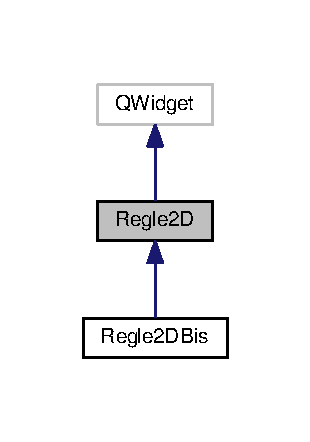
\includegraphics[width=149pt]{class_regle2_d__inherit__graph}
\end{center}
\end{figure}


Graphe de collaboration de Regle2D\+:\nopagebreak
\begin{figure}[H]
\begin{center}
\leavevmode
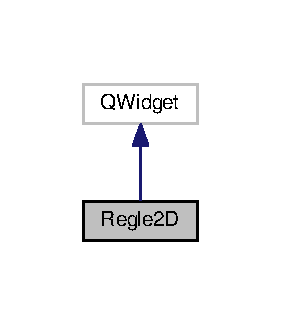
\includegraphics[width=135pt]{class_regle2_d__coll__graph}
\end{center}
\end{figure}
\subsection*{Connecteurs publics}
\begin{DoxyCompactItemize}
\item 
void \hyperlink{class_regle2_d_a832501bff71ae1739d7936caee265477}{cacher} ()
\begin{DoxyCompactList}\small\item\em S\+L\+OT qui cache les lignes inutiles en fonction du nombre d\textquotesingle{}états entré \end{DoxyCompactList}\item 
void \hyperlink{class_regle2_d_ab66521625d0ff29d5928d65b1d62b14e}{set\+Regle} ()
\begin{DoxyCompactList}\small\item\em S\+L\+OT qui affecte l\textquotesingle{}attribut membre regle pour mettre la règle dans le même format que \hyperlink{class_autocell2_d}{Autocell2D}. \end{DoxyCompactList}\item 
void \hyperlink{class_regle2_d_a9147d46c674a80a5ef969a2b7f9ad9bc}{set\+Couleur} ()
\begin{DoxyCompactList}\small\item\em S\+L\+OT qui affecte l\textquotesingle{}attribut membre couleur\+Nom pour mettre le mettre dans le même format que \hyperlink{class_autocell2_d}{Autocell2D}. \end{DoxyCompactList}\item 
void \hyperlink{class_regle2_d_a1958192093ce058d829ffc77cfa8ee78}{send\+Regle} ()
\begin{DoxyCompactList}\small\item\em S\+L\+OT qui envoie le signal envoie\+Regle. \end{DoxyCompactList}\item 
void \hyperlink{class_regle2_d_aa096e82f85ef2cfa78bf6784b5dda448}{regle\+Predefini} (Q\+String)
\begin{DoxyCompactList}\small\item\em S\+L\+OT qui gère les règles prédéfinies. \end{DoxyCompactList}\item 
virtual void \hyperlink{class_regle2_d_ad53e81ccd6fa9eb94d30d87dca19a213}{ajout\+Regle\+Predefini} (Q\+String)
\begin{DoxyCompactList}\small\item\em S\+L\+OT Hook qui permet de rajouter des règles prédéfinies. \end{DoxyCompactList}\item 
void \hyperlink{class_regle2_d_a95a59bb0ffbc2a4fd735a4695c95d72f}{montrer} ()
\begin{DoxyCompactList}\small\item\em S\+L\+OT qui montre les lignes nécessaires en fonction du nombre d\textquotesingle{}états entré \end{DoxyCompactList}\item 
void \hyperlink{class_regle2_d_ae82e185c4e126e9bee7fd2e91e29b2f0}{adjust} ()
\begin{DoxyCompactList}\small\item\em S\+L\+OT qui utilise \hyperlink{class_regle2_d_a95a59bb0ffbc2a4fd735a4695c95d72f}{montrer()} et \hyperlink{class_regle2_d_a832501bff71ae1739d7936caee265477}{cacher()} pour modifier la fenêtre en fonction du nombre d\textquotesingle{}état. \end{DoxyCompactList}\end{DoxyCompactItemize}
\subsection*{Signaux}
\begin{DoxyCompactItemize}
\item 
void \hyperlink{class_regle2_d_ae4d763e7e7dec6c1e339769ba7ec0c52}{envoi\+Regle} (std\+::vector$<$ std\+::vector$<$ unsigned short int $>$$>$, std\+::vector$<$ std\+::string $>$)
\begin{DoxyCompactList}\small\item\em S\+I\+G\+N\+AL qui envoie la règle et la couleur des cellules. \end{DoxyCompactList}\end{DoxyCompactItemize}
\subsection*{Fonctions membres publiques}
\begin{DoxyCompactItemize}
\item 
\hyperlink{class_regle2_d_a21a799e32774f6cc50183a04422498e4}{Regle2D} (Q\+Widget $\ast$parent=nullptr)
\begin{DoxyCompactList}\small\item\em Constructeur. \end{DoxyCompactList}\item 
const Q\+Spin\+Box $\ast$ \hyperlink{class_regle2_d_abce7ef62aa852352d77ce8f88d5f05b6}{get\+\_\+nb\+Etat} () const 
\begin{DoxyCompactList}\small\item\em accesseur lecture \end{DoxyCompactList}\item 
const Q\+Combo\+Box $\ast$ \hyperlink{class_regle2_d_a25aba2d5c2d9acff7f433e35cb048504}{get\+\_\+regle\+Base} () const 
\begin{DoxyCompactList}\small\item\em accesseur lecture \end{DoxyCompactList}\item 
const std\+::vector$<$ Q\+Spin\+Box $\ast$ $>$ \& \hyperlink{class_regle2_d_a78534b72823ef634bf49d5f0f9db77f6}{get\+\_\+etat\+Cellule\+Pour\+Appliquer} () const 
\begin{DoxyCompactList}\small\item\em accesseur lecture \end{DoxyCompactList}\item 
const std\+::vector$<$ Q\+Spin\+Box $\ast$ $>$ \& \hyperlink{class_regle2_d_a7659287a9161902d50ac2e92c89919e6}{get\+\_\+cellule\+A\+C\+Compter} () const 
\begin{DoxyCompactList}\small\item\em accesseur lecture \end{DoxyCompactList}\item 
const std\+::vector$<$ Q\+Combo\+Box $\ast$ $>$ \& \hyperlink{class_regle2_d_a16721b0251aaedbac6b25dc840bc3aad}{get\+\_\+interval} () const 
\begin{DoxyCompactList}\small\item\em accesseur lecture \end{DoxyCompactList}\item 
const std\+::vector$<$ Q\+Spin\+Box $\ast$ $>$ \& \hyperlink{class_regle2_d_af9719a1cd616a23bbdb3271626161aee}{get\+\_\+borne\+Inf} () const 
\begin{DoxyCompactList}\small\item\em accesseur lecture \end{DoxyCompactList}\item 
const std\+::vector$<$ Q\+Spin\+Box $\ast$ $>$ \& \hyperlink{class_regle2_d_ada123ada77ca4c432fb6793466a2f653}{get\+\_\+borne\+Sup} () const 
\begin{DoxyCompactList}\small\item\em accesseur lecture \end{DoxyCompactList}\item 
const std\+::vector$<$ Q\+Combo\+Box $\ast$ $>$ \& \hyperlink{class_regle2_d_a9da84d09974a0cf60d59bf84e4bfff0a}{get\+\_\+couleur} () const 
\begin{DoxyCompactList}\small\item\em accesseur lecture \end{DoxyCompactList}\item 
const std\+::vector$<$ std\+::string $>$ \& \hyperlink{class_regle2_d_a80dc816d0ce1dc33cba264c41e1a6f8e}{get\+\_\+couleur\+Nom} () const 
\begin{DoxyCompactList}\small\item\em accesseur lecture \end{DoxyCompactList}\item 
const std\+::vector$<$ std\+::vector$<$ unsigned short int $>$ $>$ \& \hyperlink{class_regle2_d_a6165adcd23f35308667da783c210c911}{get\+\_\+regle} () const 
\begin{DoxyCompactList}\small\item\em accesseur lecture \end{DoxyCompactList}\item 
void \hyperlink{class_regle2_d_a93a3404a450462b60a01dcf102e65eee}{set\+Regle\+Base} (const Q\+String \&s)
\begin{DoxyCompactList}\small\item\em change la règle prédéfinie \end{DoxyCompactList}\item 
void \hyperlink{class_regle2_d_aa287cec81b0b71d3f87fea5357bec46b}{set\+Nb\+Etat} (unsigned int n)
\begin{DoxyCompactList}\small\item\em change le nombre d\textquotesingle{}état \end{DoxyCompactList}\item 
void \hyperlink{class_regle2_d_adfdc1e1d68906882c9e96b900dc49086}{set\+Etat\+Cellule\+Pour\+Appliquer} (unsigned int i, unsigned int n)
\begin{DoxyCompactList}\small\item\em change l\textquotesingle{}objet à l\textquotesingle{}indice i \end{DoxyCompactList}\item 
void \hyperlink{class_regle2_d_af12aeb43af9b84670923ef55c5c1daf6}{set\+Cellule\+A\+Compter} (unsigned int i, unsigned int n)
\begin{DoxyCompactList}\small\item\em change l\textquotesingle{}objet à l\textquotesingle{}indice i \end{DoxyCompactList}\item 
void \hyperlink{class_regle2_d_a67d7b3803a63f2bb1b2b3073e01334ba}{set\+Interval} (unsigned int i, const Q\+String \&s)
\begin{DoxyCompactList}\small\item\em change l\textquotesingle{}objet à l\textquotesingle{}indice i \end{DoxyCompactList}\item 
void \hyperlink{class_regle2_d_aa547b53ccd967ba81e1eb899517713c7}{set\+Borne\+Inf} (unsigned int i, unsigned int n)
\begin{DoxyCompactList}\small\item\em change l\textquotesingle{}objet à l\textquotesingle{}indice i \end{DoxyCompactList}\item 
void \hyperlink{class_regle2_d_a65e642a8babbaf2f9ab92c105b44753c}{set\+Borne\+Sup} (unsigned int i, unsigned int n)
\begin{DoxyCompactList}\small\item\em change l\textquotesingle{}objet à l\textquotesingle{}indice i \end{DoxyCompactList}\item 
void \hyperlink{class_regle2_d_a1f45d6182d2e12d25717c8958cdffeac}{set\+Couleur} (unsigned int i, const Q\+String \&s)
\begin{DoxyCompactList}\small\item\em change l\textquotesingle{}objet à l\textquotesingle{}indice i \end{DoxyCompactList}\end{DoxyCompactItemize}
\subsection*{Fonctions membres protégées}
\begin{DoxyCompactItemize}
\item 
void \hyperlink{class_regle2_d_a89d141ceb6bca904b32c4b31a824538d}{depart} ()
\begin{DoxyCompactList}\small\item\em initialise tous les attributs méthode protected \end{DoxyCompactList}\end{DoxyCompactItemize}
\subsection*{Attributs protégés}
\begin{DoxyCompactItemize}
\item 
std\+::vector$<$ std\+::vector$<$ unsigned short int $>$ $>$ \hyperlink{class_regle2_d_adaa6396d86c6f21c6bf7ae5ba4346dde}{regle}
\item 
std\+::vector$<$ std\+::string $>$ \hyperlink{class_regle2_d_aece48b7d62d4dc0ebfc8fd7334e7d9be}{couleur\+Nom}
\item 
Q\+Spin\+Box $\ast$ \hyperlink{class_regle2_d_a2a2964b8223ff47e483f0703c482526a}{nb\+Etat}
\item 
Q\+Combo\+Box $\ast$ \hyperlink{class_regle2_d_ae544919d03302b0ecd7bfacfc2842ccf}{regle\+Base}
\item 
std\+::vector$<$ Q\+Spin\+Box $\ast$ $>$ \hyperlink{class_regle2_d_aa5356ff562ccfe9828275effb8866fa9}{etat\+Cellule\+Pour\+Appliquer}
\item 
std\+::vector$<$ Q\+Spin\+Box $\ast$ $>$ \hyperlink{class_regle2_d_aff3f269a5118bda47bcdf133d26010e6}{cellule\+A\+C\+Compter}
\item 
std\+::vector$<$ Q\+Combo\+Box $\ast$ $>$ \hyperlink{class_regle2_d_a528a7cfc33a1be6540177b67e270c157}{interval}
\item 
std\+::vector$<$ Q\+Spin\+Box $\ast$ $>$ \hyperlink{class_regle2_d_a1b15542eb7bc7b32dc9c1cc615089eab}{borne\+Inf}
\item 
std\+::vector$<$ Q\+Spin\+Box $\ast$ $>$ \hyperlink{class_regle2_d_a206e0c9c6f0710e98326e438affb2134}{borne\+Sup}
\item 
std\+::vector$<$ Q\+Combo\+Box $\ast$ $>$ \hyperlink{class_regle2_d_a57b848611ac63837d30790b5ddec9299}{couleur}
\item 
Q\+Grid\+Layout $\ast$ \hyperlink{class_regle2_d_a344f417a81ffccf34760808b3969d25e}{layout}
\end{DoxyCompactItemize}


\subsection{Description détaillée}
Hérite de Q\+Widget. La classe \hyperlink{class_regle2_d}{Regle2D} permet d\textquotesingle{}entrer une règle pour un autocell2D (classe \hyperlink{class_automate2_d}{Automate2D} et \hyperlink{class_etat2_d}{Etat2D}) 

\subsection{Documentation des constructeurs et destructeur}
\index{Regle2D@{Regle2D}!Regle2D@{Regle2D}}
\index{Regle2D@{Regle2D}!Regle2D@{Regle2D}}
\subsubsection[{\texorpdfstring{Regle2\+D(\+Q\+Widget $\ast$parent=nullptr)}{Regle2D(QWidget *parent=nullptr)}}]{\setlength{\rightskip}{0pt plus 5cm}Regle2\+D\+::\+Regle2D (
\begin{DoxyParamCaption}
\item[{Q\+Widget $\ast$}]{parent = {\ttfamily nullptr}}
\end{DoxyParamCaption}
)}\hypertarget{class_regle2_d_a21a799e32774f6cc50183a04422498e4}{}\label{class_regle2_d_a21a799e32774f6cc50183a04422498e4}


Constructeur. 



\subsection{Documentation des fonctions membres}
\index{Regle2D@{Regle2D}!adjust@{adjust}}
\index{adjust@{adjust}!Regle2D@{Regle2D}}
\subsubsection[{\texorpdfstring{adjust}{adjust}}]{\setlength{\rightskip}{0pt plus 5cm}void Regle2\+D\+::adjust (
\begin{DoxyParamCaption}
{}
\end{DoxyParamCaption}
)\hspace{0.3cm}{\ttfamily [slot]}}\hypertarget{class_regle2_d_ae82e185c4e126e9bee7fd2e91e29b2f0}{}\label{class_regle2_d_ae82e185c4e126e9bee7fd2e91e29b2f0}


S\+L\+OT qui utilise \hyperlink{class_regle2_d_a95a59bb0ffbc2a4fd735a4695c95d72f}{montrer()} et \hyperlink{class_regle2_d_a832501bff71ae1739d7936caee265477}{cacher()} pour modifier la fenêtre en fonction du nombre d\textquotesingle{}état. 

\index{Regle2D@{Regle2D}!ajout\+Regle\+Predefini@{ajout\+Regle\+Predefini}}
\index{ajout\+Regle\+Predefini@{ajout\+Regle\+Predefini}!Regle2D@{Regle2D}}
\subsubsection[{\texorpdfstring{ajout\+Regle\+Predefini}{ajoutReglePredefini}}]{\setlength{\rightskip}{0pt plus 5cm}void Regle2\+D\+::ajout\+Regle\+Predefini (
\begin{DoxyParamCaption}
\item[{Q\+String}]{}
\end{DoxyParamCaption}
)\hspace{0.3cm}{\ttfamily [virtual]}, {\ttfamily [slot]}}\hypertarget{class_regle2_d_ad53e81ccd6fa9eb94d30d87dca19a213}{}\label{class_regle2_d_ad53e81ccd6fa9eb94d30d87dca19a213}


S\+L\+OT Hook qui permet de rajouter des règles prédéfinies. 



Réimplémentée dans \hyperlink{class_regle2_d_bis_a7851a6efdc011876e729797fc70e0a0f}{Regle2\+D\+Bis}.

\index{Regle2D@{Regle2D}!cacher@{cacher}}
\index{cacher@{cacher}!Regle2D@{Regle2D}}
\subsubsection[{\texorpdfstring{cacher}{cacher}}]{\setlength{\rightskip}{0pt plus 5cm}void Regle2\+D\+::cacher (
\begin{DoxyParamCaption}
{}
\end{DoxyParamCaption}
)\hspace{0.3cm}{\ttfamily [slot]}}\hypertarget{class_regle2_d_a832501bff71ae1739d7936caee265477}{}\label{class_regle2_d_a832501bff71ae1739d7936caee265477}


S\+L\+OT qui cache les lignes inutiles en fonction du nombre d\textquotesingle{}états entré 

\index{Regle2D@{Regle2D}!depart@{depart}}
\index{depart@{depart}!Regle2D@{Regle2D}}
\subsubsection[{\texorpdfstring{depart()}{depart()}}]{\setlength{\rightskip}{0pt plus 5cm}void Regle2\+D\+::depart (
\begin{DoxyParamCaption}
{}
\end{DoxyParamCaption}
)\hspace{0.3cm}{\ttfamily [protected]}}\hypertarget{class_regle2_d_a89d141ceb6bca904b32c4b31a824538d}{}\label{class_regle2_d_a89d141ceb6bca904b32c4b31a824538d}


initialise tous les attributs méthode protected 

\index{Regle2D@{Regle2D}!envoi\+Regle@{envoi\+Regle}}
\index{envoi\+Regle@{envoi\+Regle}!Regle2D@{Regle2D}}
\subsubsection[{\texorpdfstring{envoi\+Regle}{envoiRegle}}]{\setlength{\rightskip}{0pt plus 5cm}void Regle2\+D\+::envoi\+Regle (
\begin{DoxyParamCaption}
\item[{std\+::vector$<$ std\+::vector$<$ unsigned short int $>$$>$}]{\+\_\+t1, }
\item[{std\+::vector$<$ std\+::string $>$}]{\+\_\+t2}
\end{DoxyParamCaption}
)\hspace{0.3cm}{\ttfamily [signal]}}\hypertarget{class_regle2_d_ae4d763e7e7dec6c1e339769ba7ec0c52}{}\label{class_regle2_d_ae4d763e7e7dec6c1e339769ba7ec0c52}


S\+I\+G\+N\+AL qui envoie la règle et la couleur des cellules. 


\begin{DoxyParams}{Paramètres}
{\em regle} & \+: std\+::vector$<$std\+::vector$<$unsigned short int$>$$>$ \\
\hline
{\em couleur} & \+: std\+::vector$<$std\+::string$>$ \\
\hline
\end{DoxyParams}
\index{Regle2D@{Regle2D}!get\+\_\+borne\+Inf@{get\+\_\+borne\+Inf}}
\index{get\+\_\+borne\+Inf@{get\+\_\+borne\+Inf}!Regle2D@{Regle2D}}
\subsubsection[{\texorpdfstring{get\+\_\+borne\+Inf() const }{get_borneInf() const }}]{\setlength{\rightskip}{0pt plus 5cm}const std\+::vector$<$Q\+Spin\+Box$\ast$$>$\& Regle2\+D\+::get\+\_\+borne\+Inf (
\begin{DoxyParamCaption}
{}
\end{DoxyParamCaption}
) const\hspace{0.3cm}{\ttfamily [inline]}}\hypertarget{class_regle2_d_af9719a1cd616a23bbdb3271626161aee}{}\label{class_regle2_d_af9719a1cd616a23bbdb3271626161aee}


accesseur lecture 

\begin{DoxyReturn}{Renvoie}
borne\+Inf \+: const std\+::vector$<$\+Q\+Spin\+Box$\ast$$>$\& 
\end{DoxyReturn}
\index{Regle2D@{Regle2D}!get\+\_\+borne\+Sup@{get\+\_\+borne\+Sup}}
\index{get\+\_\+borne\+Sup@{get\+\_\+borne\+Sup}!Regle2D@{Regle2D}}
\subsubsection[{\texorpdfstring{get\+\_\+borne\+Sup() const }{get_borneSup() const }}]{\setlength{\rightskip}{0pt plus 5cm}const std\+::vector$<$Q\+Spin\+Box$\ast$$>$\& Regle2\+D\+::get\+\_\+borne\+Sup (
\begin{DoxyParamCaption}
{}
\end{DoxyParamCaption}
) const\hspace{0.3cm}{\ttfamily [inline]}}\hypertarget{class_regle2_d_ada123ada77ca4c432fb6793466a2f653}{}\label{class_regle2_d_ada123ada77ca4c432fb6793466a2f653}


accesseur lecture 

\begin{DoxyReturn}{Renvoie}
borne\+Sup \+: const std\+::vector$<$\+Q\+Spin\+Box$\ast$$>$\& 
\end{DoxyReturn}
\index{Regle2D@{Regle2D}!get\+\_\+cellule\+A\+C\+Compter@{get\+\_\+cellule\+A\+C\+Compter}}
\index{get\+\_\+cellule\+A\+C\+Compter@{get\+\_\+cellule\+A\+C\+Compter}!Regle2D@{Regle2D}}
\subsubsection[{\texorpdfstring{get\+\_\+cellule\+A\+C\+Compter() const }{get_celluleACCompter() const }}]{\setlength{\rightskip}{0pt plus 5cm}const std\+::vector$<$Q\+Spin\+Box$\ast$$>$\& Regle2\+D\+::get\+\_\+cellule\+A\+C\+Compter (
\begin{DoxyParamCaption}
{}
\end{DoxyParamCaption}
) const\hspace{0.3cm}{\ttfamily [inline]}}\hypertarget{class_regle2_d_a7659287a9161902d50ac2e92c89919e6}{}\label{class_regle2_d_a7659287a9161902d50ac2e92c89919e6}


accesseur lecture 

\begin{DoxyReturn}{Renvoie}
cellule\+A\+C\+Compter \+: const std\+::vector$<$\+Q\+Spin\+Box$\ast$$>$\& 
\end{DoxyReturn}
\index{Regle2D@{Regle2D}!get\+\_\+couleur@{get\+\_\+couleur}}
\index{get\+\_\+couleur@{get\+\_\+couleur}!Regle2D@{Regle2D}}
\subsubsection[{\texorpdfstring{get\+\_\+couleur() const }{get_couleur() const }}]{\setlength{\rightskip}{0pt plus 5cm}const std\+::vector$<$Q\+Combo\+Box$\ast$$>$\& Regle2\+D\+::get\+\_\+couleur (
\begin{DoxyParamCaption}
{}
\end{DoxyParamCaption}
) const\hspace{0.3cm}{\ttfamily [inline]}}\hypertarget{class_regle2_d_a9da84d09974a0cf60d59bf84e4bfff0a}{}\label{class_regle2_d_a9da84d09974a0cf60d59bf84e4bfff0a}


accesseur lecture 

\begin{DoxyReturn}{Renvoie}
couleur \+: const std\+::vector$<$\+Q\+Combo\+Box$\ast$$>$\& 
\end{DoxyReturn}
\index{Regle2D@{Regle2D}!get\+\_\+couleur\+Nom@{get\+\_\+couleur\+Nom}}
\index{get\+\_\+couleur\+Nom@{get\+\_\+couleur\+Nom}!Regle2D@{Regle2D}}
\subsubsection[{\texorpdfstring{get\+\_\+couleur\+Nom() const }{get_couleurNom() const }}]{\setlength{\rightskip}{0pt plus 5cm}const std\+::vector$<$std\+::string$>$\& Regle2\+D\+::get\+\_\+couleur\+Nom (
\begin{DoxyParamCaption}
{}
\end{DoxyParamCaption}
) const\hspace{0.3cm}{\ttfamily [inline]}}\hypertarget{class_regle2_d_a80dc816d0ce1dc33cba264c41e1a6f8e}{}\label{class_regle2_d_a80dc816d0ce1dc33cba264c41e1a6f8e}


accesseur lecture 

\begin{DoxyReturn}{Renvoie}
couleur\+Nom \+: const std\+::vector$<$std\+::string$>$\& 
\end{DoxyReturn}
\index{Regle2D@{Regle2D}!get\+\_\+etat\+Cellule\+Pour\+Appliquer@{get\+\_\+etat\+Cellule\+Pour\+Appliquer}}
\index{get\+\_\+etat\+Cellule\+Pour\+Appliquer@{get\+\_\+etat\+Cellule\+Pour\+Appliquer}!Regle2D@{Regle2D}}
\subsubsection[{\texorpdfstring{get\+\_\+etat\+Cellule\+Pour\+Appliquer() const }{get_etatCellulePourAppliquer() const }}]{\setlength{\rightskip}{0pt plus 5cm}const std\+::vector$<$Q\+Spin\+Box$\ast$$>$\& Regle2\+D\+::get\+\_\+etat\+Cellule\+Pour\+Appliquer (
\begin{DoxyParamCaption}
{}
\end{DoxyParamCaption}
) const\hspace{0.3cm}{\ttfamily [inline]}}\hypertarget{class_regle2_d_a78534b72823ef634bf49d5f0f9db77f6}{}\label{class_regle2_d_a78534b72823ef634bf49d5f0f9db77f6}


accesseur lecture 

\begin{DoxyReturn}{Renvoie}
etat\+Cellule\+Pour\+Appliquer \+: const std\+::vector$<$\+Q\+Spin\+Box$\ast$$>$\& 
\end{DoxyReturn}
\index{Regle2D@{Regle2D}!get\+\_\+interval@{get\+\_\+interval}}
\index{get\+\_\+interval@{get\+\_\+interval}!Regle2D@{Regle2D}}
\subsubsection[{\texorpdfstring{get\+\_\+interval() const }{get_interval() const }}]{\setlength{\rightskip}{0pt plus 5cm}const std\+::vector$<$Q\+Combo\+Box$\ast$$>$\& Regle2\+D\+::get\+\_\+interval (
\begin{DoxyParamCaption}
{}
\end{DoxyParamCaption}
) const\hspace{0.3cm}{\ttfamily [inline]}}\hypertarget{class_regle2_d_a16721b0251aaedbac6b25dc840bc3aad}{}\label{class_regle2_d_a16721b0251aaedbac6b25dc840bc3aad}


accesseur lecture 

\begin{DoxyReturn}{Renvoie}
interval \+: const std\+::vector$<$\+Q\+Combo\+Box$\ast$$>$\& 
\end{DoxyReturn}
\index{Regle2D@{Regle2D}!get\+\_\+nb\+Etat@{get\+\_\+nb\+Etat}}
\index{get\+\_\+nb\+Etat@{get\+\_\+nb\+Etat}!Regle2D@{Regle2D}}
\subsubsection[{\texorpdfstring{get\+\_\+nb\+Etat() const }{get_nbEtat() const }}]{\setlength{\rightskip}{0pt plus 5cm}const Q\+Spin\+Box$\ast$ Regle2\+D\+::get\+\_\+nb\+Etat (
\begin{DoxyParamCaption}
{}
\end{DoxyParamCaption}
) const\hspace{0.3cm}{\ttfamily [inline]}}\hypertarget{class_regle2_d_abce7ef62aa852352d77ce8f88d5f05b6}{}\label{class_regle2_d_abce7ef62aa852352d77ce8f88d5f05b6}


accesseur lecture 

\begin{DoxyReturn}{Renvoie}
nb\+Etat \+: const Q\+Spin\+Box$\ast$ 
\end{DoxyReturn}
\index{Regle2D@{Regle2D}!get\+\_\+regle@{get\+\_\+regle}}
\index{get\+\_\+regle@{get\+\_\+regle}!Regle2D@{Regle2D}}
\subsubsection[{\texorpdfstring{get\+\_\+regle() const }{get_regle() const }}]{\setlength{\rightskip}{0pt plus 5cm}const std\+::vector$<$std\+::vector$<$unsigned short int$>$ $>$\& Regle2\+D\+::get\+\_\+regle (
\begin{DoxyParamCaption}
{}
\end{DoxyParamCaption}
) const\hspace{0.3cm}{\ttfamily [inline]}}\hypertarget{class_regle2_d_a6165adcd23f35308667da783c210c911}{}\label{class_regle2_d_a6165adcd23f35308667da783c210c911}


accesseur lecture 

\begin{DoxyReturn}{Renvoie}
regle \+: const std\+::vector$<$std\+::vector$<$unsigned short int$>$$>$\& 
\end{DoxyReturn}
\index{Regle2D@{Regle2D}!get\+\_\+regle\+Base@{get\+\_\+regle\+Base}}
\index{get\+\_\+regle\+Base@{get\+\_\+regle\+Base}!Regle2D@{Regle2D}}
\subsubsection[{\texorpdfstring{get\+\_\+regle\+Base() const }{get_regleBase() const }}]{\setlength{\rightskip}{0pt plus 5cm}const Q\+Combo\+Box$\ast$ Regle2\+D\+::get\+\_\+regle\+Base (
\begin{DoxyParamCaption}
{}
\end{DoxyParamCaption}
) const\hspace{0.3cm}{\ttfamily [inline]}}\hypertarget{class_regle2_d_a25aba2d5c2d9acff7f433e35cb048504}{}\label{class_regle2_d_a25aba2d5c2d9acff7f433e35cb048504}


accesseur lecture 

\begin{DoxyReturn}{Renvoie}
regle\+Base \+: const Q\+Combo\+Box$\ast$ 
\end{DoxyReturn}
\index{Regle2D@{Regle2D}!montrer@{montrer}}
\index{montrer@{montrer}!Regle2D@{Regle2D}}
\subsubsection[{\texorpdfstring{montrer}{montrer}}]{\setlength{\rightskip}{0pt plus 5cm}void Regle2\+D\+::montrer (
\begin{DoxyParamCaption}
{}
\end{DoxyParamCaption}
)\hspace{0.3cm}{\ttfamily [slot]}}\hypertarget{class_regle2_d_a95a59bb0ffbc2a4fd735a4695c95d72f}{}\label{class_regle2_d_a95a59bb0ffbc2a4fd735a4695c95d72f}


S\+L\+OT qui montre les lignes nécessaires en fonction du nombre d\textquotesingle{}états entré 

\index{Regle2D@{Regle2D}!regle\+Predefini@{regle\+Predefini}}
\index{regle\+Predefini@{regle\+Predefini}!Regle2D@{Regle2D}}
\subsubsection[{\texorpdfstring{regle\+Predefini}{reglePredefini}}]{\setlength{\rightskip}{0pt plus 5cm}void Regle2\+D\+::regle\+Predefini (
\begin{DoxyParamCaption}
\item[{Q\+String}]{nom}
\end{DoxyParamCaption}
)\hspace{0.3cm}{\ttfamily [slot]}}\hypertarget{class_regle2_d_aa096e82f85ef2cfa78bf6784b5dda448}{}\label{class_regle2_d_aa096e82f85ef2cfa78bf6784b5dda448}


S\+L\+OT qui gère les règles prédéfinies. 

\index{Regle2D@{Regle2D}!send\+Regle@{send\+Regle}}
\index{send\+Regle@{send\+Regle}!Regle2D@{Regle2D}}
\subsubsection[{\texorpdfstring{send\+Regle}{sendRegle}}]{\setlength{\rightskip}{0pt plus 5cm}void Regle2\+D\+::send\+Regle (
\begin{DoxyParamCaption}
{}
\end{DoxyParamCaption}
)\hspace{0.3cm}{\ttfamily [slot]}}\hypertarget{class_regle2_d_a1958192093ce058d829ffc77cfa8ee78}{}\label{class_regle2_d_a1958192093ce058d829ffc77cfa8ee78}


S\+L\+OT qui envoie le signal envoie\+Regle. 

\index{Regle2D@{Regle2D}!set\+Borne\+Inf@{set\+Borne\+Inf}}
\index{set\+Borne\+Inf@{set\+Borne\+Inf}!Regle2D@{Regle2D}}
\subsubsection[{\texorpdfstring{set\+Borne\+Inf(unsigned int i, unsigned int n)}{setBorneInf(unsigned int i, unsigned int n)}}]{\setlength{\rightskip}{0pt plus 5cm}void Regle2\+D\+::set\+Borne\+Inf (
\begin{DoxyParamCaption}
\item[{unsigned int}]{i, }
\item[{unsigned int}]{n}
\end{DoxyParamCaption}
)\hspace{0.3cm}{\ttfamily [inline]}}\hypertarget{class_regle2_d_aa547b53ccd967ba81e1eb899517713c7}{}\label{class_regle2_d_aa547b53ccd967ba81e1eb899517713c7}


change l\textquotesingle{}objet à l\textquotesingle{}indice i 


\begin{DoxyParams}{Paramètres}
{\em i} & \+: indice \+: unsigned int \\
\hline
{\em n} & \+: nouvelle valeur \+: unsigned int \\
\hline
\end{DoxyParams}
\index{Regle2D@{Regle2D}!set\+Borne\+Sup@{set\+Borne\+Sup}}
\index{set\+Borne\+Sup@{set\+Borne\+Sup}!Regle2D@{Regle2D}}
\subsubsection[{\texorpdfstring{set\+Borne\+Sup(unsigned int i, unsigned int n)}{setBorneSup(unsigned int i, unsigned int n)}}]{\setlength{\rightskip}{0pt plus 5cm}void Regle2\+D\+::set\+Borne\+Sup (
\begin{DoxyParamCaption}
\item[{unsigned int}]{i, }
\item[{unsigned int}]{n}
\end{DoxyParamCaption}
)\hspace{0.3cm}{\ttfamily [inline]}}\hypertarget{class_regle2_d_a65e642a8babbaf2f9ab92c105b44753c}{}\label{class_regle2_d_a65e642a8babbaf2f9ab92c105b44753c}


change l\textquotesingle{}objet à l\textquotesingle{}indice i 


\begin{DoxyParams}{Paramètres}
{\em i} & \+: indice \+: unsigned int \\
\hline
{\em n} & \+: nouvelle valeur \+: unsigned int \\
\hline
\end{DoxyParams}
\index{Regle2D@{Regle2D}!set\+Cellule\+A\+Compter@{set\+Cellule\+A\+Compter}}
\index{set\+Cellule\+A\+Compter@{set\+Cellule\+A\+Compter}!Regle2D@{Regle2D}}
\subsubsection[{\texorpdfstring{set\+Cellule\+A\+Compter(unsigned int i, unsigned int n)}{setCelluleACompter(unsigned int i, unsigned int n)}}]{\setlength{\rightskip}{0pt plus 5cm}void Regle2\+D\+::set\+Cellule\+A\+Compter (
\begin{DoxyParamCaption}
\item[{unsigned int}]{i, }
\item[{unsigned int}]{n}
\end{DoxyParamCaption}
)\hspace{0.3cm}{\ttfamily [inline]}}\hypertarget{class_regle2_d_af12aeb43af9b84670923ef55c5c1daf6}{}\label{class_regle2_d_af12aeb43af9b84670923ef55c5c1daf6}


change l\textquotesingle{}objet à l\textquotesingle{}indice i 


\begin{DoxyParams}{Paramètres}
{\em i} & \+: indice \+: unsigned int \\
\hline
{\em n} & \+: nouvelle valeur \+: unsigned int \\
\hline
\end{DoxyParams}
\index{Regle2D@{Regle2D}!set\+Couleur@{set\+Couleur}}
\index{set\+Couleur@{set\+Couleur}!Regle2D@{Regle2D}}
\subsubsection[{\texorpdfstring{set\+Couleur(unsigned int i, const Q\+String \&s)}{setCouleur(unsigned int i, const QString &s)}}]{\setlength{\rightskip}{0pt plus 5cm}void Regle2\+D\+::set\+Couleur (
\begin{DoxyParamCaption}
\item[{unsigned int}]{i, }
\item[{const Q\+String \&}]{s}
\end{DoxyParamCaption}
)\hspace{0.3cm}{\ttfamily [inline]}}\hypertarget{class_regle2_d_a1f45d6182d2e12d25717c8958cdffeac}{}\label{class_regle2_d_a1f45d6182d2e12d25717c8958cdffeac}


change l\textquotesingle{}objet à l\textquotesingle{}indice i 


\begin{DoxyParams}{Paramètres}
{\em i} & \+: indice \+: unsigned int \\
\hline
{\em s} & \+: nouvelle valeur \+: const Q\+String\& \\
\hline
\end{DoxyParams}
\index{Regle2D@{Regle2D}!set\+Couleur@{set\+Couleur}}
\index{set\+Couleur@{set\+Couleur}!Regle2D@{Regle2D}}
\subsubsection[{\texorpdfstring{set\+Couleur}{setCouleur}}]{\setlength{\rightskip}{0pt plus 5cm}void Regle2\+D\+::set\+Couleur (
\begin{DoxyParamCaption}
{}
\end{DoxyParamCaption}
)\hspace{0.3cm}{\ttfamily [slot]}}\hypertarget{class_regle2_d_a9147d46c674a80a5ef969a2b7f9ad9bc}{}\label{class_regle2_d_a9147d46c674a80a5ef969a2b7f9ad9bc}


S\+L\+OT qui affecte l\textquotesingle{}attribut membre couleur\+Nom pour mettre le mettre dans le même format que \hyperlink{class_autocell2_d}{Autocell2D}. 

\index{Regle2D@{Regle2D}!set\+Etat\+Cellule\+Pour\+Appliquer@{set\+Etat\+Cellule\+Pour\+Appliquer}}
\index{set\+Etat\+Cellule\+Pour\+Appliquer@{set\+Etat\+Cellule\+Pour\+Appliquer}!Regle2D@{Regle2D}}
\subsubsection[{\texorpdfstring{set\+Etat\+Cellule\+Pour\+Appliquer(unsigned int i, unsigned int n)}{setEtatCellulePourAppliquer(unsigned int i, unsigned int n)}}]{\setlength{\rightskip}{0pt plus 5cm}void Regle2\+D\+::set\+Etat\+Cellule\+Pour\+Appliquer (
\begin{DoxyParamCaption}
\item[{unsigned int}]{i, }
\item[{unsigned int}]{n}
\end{DoxyParamCaption}
)\hspace{0.3cm}{\ttfamily [inline]}}\hypertarget{class_regle2_d_adfdc1e1d68906882c9e96b900dc49086}{}\label{class_regle2_d_adfdc1e1d68906882c9e96b900dc49086}


change l\textquotesingle{}objet à l\textquotesingle{}indice i 


\begin{DoxyParams}{Paramètres}
{\em i} & \+: indice \+: unsigned int \\
\hline
{\em n} & \+: nouvelle valeur \+: unsigned int \\
\hline
\end{DoxyParams}
\index{Regle2D@{Regle2D}!set\+Interval@{set\+Interval}}
\index{set\+Interval@{set\+Interval}!Regle2D@{Regle2D}}
\subsubsection[{\texorpdfstring{set\+Interval(unsigned int i, const Q\+String \&s)}{setInterval(unsigned int i, const QString &s)}}]{\setlength{\rightskip}{0pt plus 5cm}void Regle2\+D\+::set\+Interval (
\begin{DoxyParamCaption}
\item[{unsigned int}]{i, }
\item[{const Q\+String \&}]{s}
\end{DoxyParamCaption}
)\hspace{0.3cm}{\ttfamily [inline]}}\hypertarget{class_regle2_d_a67d7b3803a63f2bb1b2b3073e01334ba}{}\label{class_regle2_d_a67d7b3803a63f2bb1b2b3073e01334ba}


change l\textquotesingle{}objet à l\textquotesingle{}indice i 


\begin{DoxyParams}{Paramètres}
{\em i} & \+: indice \+: unsigned int \\
\hline
{\em s} & \+: nouvelle valeur \+: const Q\+String\& \\
\hline
\end{DoxyParams}
\index{Regle2D@{Regle2D}!set\+Nb\+Etat@{set\+Nb\+Etat}}
\index{set\+Nb\+Etat@{set\+Nb\+Etat}!Regle2D@{Regle2D}}
\subsubsection[{\texorpdfstring{set\+Nb\+Etat(unsigned int n)}{setNbEtat(unsigned int n)}}]{\setlength{\rightskip}{0pt plus 5cm}void Regle2\+D\+::set\+Nb\+Etat (
\begin{DoxyParamCaption}
\item[{unsigned int}]{n}
\end{DoxyParamCaption}
)\hspace{0.3cm}{\ttfamily [inline]}}\hypertarget{class_regle2_d_aa287cec81b0b71d3f87fea5357bec46b}{}\label{class_regle2_d_aa287cec81b0b71d3f87fea5357bec46b}


change le nombre d\textquotesingle{}état 


\begin{DoxyParams}{Paramètres}
{\em n} & \+: nouveau nombre d\textquotesingle{}état\+: unsigned int \\
\hline
\end{DoxyParams}
\index{Regle2D@{Regle2D}!set\+Regle@{set\+Regle}}
\index{set\+Regle@{set\+Regle}!Regle2D@{Regle2D}}
\subsubsection[{\texorpdfstring{set\+Regle}{setRegle}}]{\setlength{\rightskip}{0pt plus 5cm}void Regle2\+D\+::set\+Regle (
\begin{DoxyParamCaption}
{}
\end{DoxyParamCaption}
)\hspace{0.3cm}{\ttfamily [slot]}}\hypertarget{class_regle2_d_ab66521625d0ff29d5928d65b1d62b14e}{}\label{class_regle2_d_ab66521625d0ff29d5928d65b1d62b14e}


S\+L\+OT qui affecte l\textquotesingle{}attribut membre regle pour mettre la règle dans le même format que \hyperlink{class_autocell2_d}{Autocell2D}. 

\index{Regle2D@{Regle2D}!set\+Regle\+Base@{set\+Regle\+Base}}
\index{set\+Regle\+Base@{set\+Regle\+Base}!Regle2D@{Regle2D}}
\subsubsection[{\texorpdfstring{set\+Regle\+Base(const Q\+String \&s)}{setRegleBase(const QString &s)}}]{\setlength{\rightskip}{0pt plus 5cm}void Regle2\+D\+::set\+Regle\+Base (
\begin{DoxyParamCaption}
\item[{const Q\+String \&}]{s}
\end{DoxyParamCaption}
)\hspace{0.3cm}{\ttfamily [inline]}}\hypertarget{class_regle2_d_a93a3404a450462b60a01dcf102e65eee}{}\label{class_regle2_d_a93a3404a450462b60a01dcf102e65eee}


change la règle prédéfinie 


\begin{DoxyParams}{Paramètres}
{\em s} & \+: nouveau nom de règle prédéfinie\+: Q\+String \\
\hline
\end{DoxyParams}


\subsection{Documentation des données membres}
\index{Regle2D@{Regle2D}!borne\+Inf@{borne\+Inf}}
\index{borne\+Inf@{borne\+Inf}!Regle2D@{Regle2D}}
\subsubsection[{\texorpdfstring{borne\+Inf}{borneInf}}]{\setlength{\rightskip}{0pt plus 5cm}std\+::vector$<$Q\+Spin\+Box$\ast$$>$ Regle2\+D\+::borne\+Inf\hspace{0.3cm}{\ttfamily [protected]}}\hypertarget{class_regle2_d_a1b15542eb7bc7b32dc9c1cc615089eab}{}\label{class_regle2_d_a1b15542eb7bc7b32dc9c1cc615089eab}
permet de rentrer la borne inférieur de l\textquotesingle{}interval \index{Regle2D@{Regle2D}!borne\+Sup@{borne\+Sup}}
\index{borne\+Sup@{borne\+Sup}!Regle2D@{Regle2D}}
\subsubsection[{\texorpdfstring{borne\+Sup}{borneSup}}]{\setlength{\rightskip}{0pt plus 5cm}std\+::vector$<$Q\+Spin\+Box$\ast$$>$ Regle2\+D\+::borne\+Sup\hspace{0.3cm}{\ttfamily [protected]}}\hypertarget{class_regle2_d_a206e0c9c6f0710e98326e438affb2134}{}\label{class_regle2_d_a206e0c9c6f0710e98326e438affb2134}
permet de rentrer la borne supérieur de l\textquotesingle{}interval \index{Regle2D@{Regle2D}!cellule\+A\+C\+Compter@{cellule\+A\+C\+Compter}}
\index{cellule\+A\+C\+Compter@{cellule\+A\+C\+Compter}!Regle2D@{Regle2D}}
\subsubsection[{\texorpdfstring{cellule\+A\+C\+Compter}{celluleACCompter}}]{\setlength{\rightskip}{0pt plus 5cm}std\+::vector$<$Q\+Spin\+Box$\ast$$>$ Regle2\+D\+::cellule\+A\+C\+Compter\hspace{0.3cm}{\ttfamily [protected]}}\hypertarget{class_regle2_d_aff3f269a5118bda47bcdf133d26010e6}{}\label{class_regle2_d_aff3f269a5118bda47bcdf133d26010e6}
permet de rentre l\textquotesingle{}état que la cellule doit avoir qu\textquotesingle{}on la considère dans l\textquotesingle{}entourage \index{Regle2D@{Regle2D}!couleur@{couleur}}
\index{couleur@{couleur}!Regle2D@{Regle2D}}
\subsubsection[{\texorpdfstring{couleur}{couleur}}]{\setlength{\rightskip}{0pt plus 5cm}std\+::vector$<$Q\+Combo\+Box$\ast$$>$ Regle2\+D\+::couleur\hspace{0.3cm}{\ttfamily [protected]}}\hypertarget{class_regle2_d_a57b848611ac63837d30790b5ddec9299}{}\label{class_regle2_d_a57b848611ac63837d30790b5ddec9299}
permet de rentrer la couleur de la cellule \index{Regle2D@{Regle2D}!couleur\+Nom@{couleur\+Nom}}
\index{couleur\+Nom@{couleur\+Nom}!Regle2D@{Regle2D}}
\subsubsection[{\texorpdfstring{couleur\+Nom}{couleurNom}}]{\setlength{\rightskip}{0pt plus 5cm}std\+::vector$<$std\+::string$>$ Regle2\+D\+::couleur\+Nom\hspace{0.3cm}{\ttfamily [protected]}}\hypertarget{class_regle2_d_aece48b7d62d4dc0ebfc8fd7334e7d9be}{}\label{class_regle2_d_aece48b7d62d4dc0ebfc8fd7334e7d9be}
enregistre les couleurs sous le même format que dans autocell2D \index{Regle2D@{Regle2D}!etat\+Cellule\+Pour\+Appliquer@{etat\+Cellule\+Pour\+Appliquer}}
\index{etat\+Cellule\+Pour\+Appliquer@{etat\+Cellule\+Pour\+Appliquer}!Regle2D@{Regle2D}}
\subsubsection[{\texorpdfstring{etat\+Cellule\+Pour\+Appliquer}{etatCellulePourAppliquer}}]{\setlength{\rightskip}{0pt plus 5cm}std\+::vector$<$Q\+Spin\+Box$\ast$$>$ Regle2\+D\+::etat\+Cellule\+Pour\+Appliquer\hspace{0.3cm}{\ttfamily [protected]}}\hypertarget{class_regle2_d_aa5356ff562ccfe9828275effb8866fa9}{}\label{class_regle2_d_aa5356ff562ccfe9828275effb8866fa9}
permet de rentre l\textquotesingle{}état que la cellule doit avoir pour qu\textquotesingle{}on lui applique la règle \index{Regle2D@{Regle2D}!interval@{interval}}
\index{interval@{interval}!Regle2D@{Regle2D}}
\subsubsection[{\texorpdfstring{interval}{interval}}]{\setlength{\rightskip}{0pt plus 5cm}std\+::vector$<$Q\+Combo\+Box$\ast$$>$ Regle2\+D\+::interval\hspace{0.3cm}{\ttfamily [protected]}}\hypertarget{class_regle2_d_a528a7cfc33a1be6540177b67e270c157}{}\label{class_regle2_d_a528a7cfc33a1be6540177b67e270c157}
permet de savoir si on doit être dedans ou hors de l\textquotesingle{}interval \index{Regle2D@{Regle2D}!layout@{layout}}
\index{layout@{layout}!Regle2D@{Regle2D}}
\subsubsection[{\texorpdfstring{layout}{layout}}]{\setlength{\rightskip}{0pt plus 5cm}Q\+Grid\+Layout$\ast$ Regle2\+D\+::layout\hspace{0.3cm}{\ttfamily [protected]}}\hypertarget{class_regle2_d_a344f417a81ffccf34760808b3969d25e}{}\label{class_regle2_d_a344f417a81ffccf34760808b3969d25e}
layout principal \index{Regle2D@{Regle2D}!nb\+Etat@{nb\+Etat}}
\index{nb\+Etat@{nb\+Etat}!Regle2D@{Regle2D}}
\subsubsection[{\texorpdfstring{nb\+Etat}{nbEtat}}]{\setlength{\rightskip}{0pt plus 5cm}Q\+Spin\+Box$\ast$ Regle2\+D\+::nb\+Etat\hspace{0.3cm}{\ttfamily [protected]}}\hypertarget{class_regle2_d_a2a2964b8223ff47e483f0703c482526a}{}\label{class_regle2_d_a2a2964b8223ff47e483f0703c482526a}
permet d\textquotesingle{}entrer le nombre d\textquotesingle{}état des cellules \index{Regle2D@{Regle2D}!regle@{regle}}
\index{regle@{regle}!Regle2D@{Regle2D}}
\subsubsection[{\texorpdfstring{regle}{regle}}]{\setlength{\rightskip}{0pt plus 5cm}std\+::vector$<$std\+::vector$<$unsigned short int$>$ $>$ Regle2\+D\+::regle\hspace{0.3cm}{\ttfamily [protected]}}\hypertarget{class_regle2_d_adaa6396d86c6f21c6bf7ae5ba4346dde}{}\label{class_regle2_d_adaa6396d86c6f21c6bf7ae5ba4346dde}
enregistre la règle sous le même format que dans autocell2D \index{Regle2D@{Regle2D}!regle\+Base@{regle\+Base}}
\index{regle\+Base@{regle\+Base}!Regle2D@{Regle2D}}
\subsubsection[{\texorpdfstring{regle\+Base}{regleBase}}]{\setlength{\rightskip}{0pt plus 5cm}Q\+Combo\+Box$\ast$ Regle2\+D\+::regle\+Base\hspace{0.3cm}{\ttfamily [protected]}}\hypertarget{class_regle2_d_ae544919d03302b0ecd7bfacfc2842ccf}{}\label{class_regle2_d_ae544919d03302b0ecd7bfacfc2842ccf}
permet de sélectionner des règles prédéfinies 

La documentation de cette classe a été générée à partir des fichiers suivants \+:\begin{DoxyCompactItemize}
\item 
info/\+L\+O21/\+L\+O21/\+Auto\+Cell/\hyperlink{autocell_8h}{autocell.\+h}\item 
info/\+L\+O21/\+L\+O21/\+Auto\+Cell/\hyperlink{autocell_8cpp}{autocell.\+cpp}\item 
info/\+L\+O21/\+L\+O21/build-\/\+Auto\+Cell-\/\+Desktop-\/\+Debug/\hyperlink{moc__autocell_8cpp}{moc\+\_\+autocell.\+cpp}\end{DoxyCompactItemize}

\hypertarget{class_regle2_d_bis}{}\section{Référence de la classe Regle2\+D\+Bis}
\label{class_regle2_d_bis}\index{Regle2\+D\+Bis@{Regle2\+D\+Bis}}


Hérite de \hyperlink{class_regle2_d}{Regle2D} La classe \hyperlink{class_regle2_d_bis}{Regle2\+D\+Bis} montre comment intégrer de nouvelles règles à un autocell2D.  




{\ttfamily \#include $<$autocell.\+h$>$}



Graphe d\textquotesingle{}héritage de Regle2\+D\+Bis\+:\nopagebreak
\begin{figure}[H]
\begin{center}
\leavevmode
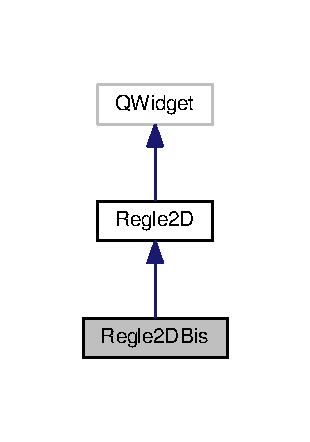
\includegraphics[width=149pt]{class_regle2_d_bis__inherit__graph}
\end{center}
\end{figure}


Graphe de collaboration de Regle2\+D\+Bis\+:\nopagebreak
\begin{figure}[H]
\begin{center}
\leavevmode
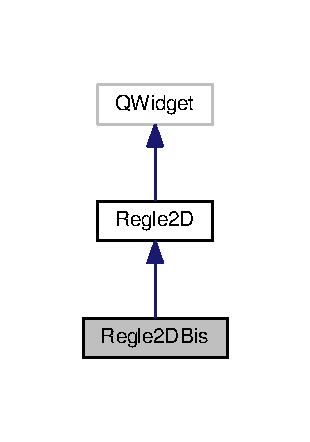
\includegraphics[width=149pt]{class_regle2_d_bis__coll__graph}
\end{center}
\end{figure}
\subsection*{Fonctions membres publiques}
\begin{DoxyCompactItemize}
\item 
\hyperlink{class_regle2_d_bis_a433953483349852ab6c9532b1d1d6489}{Regle2\+D\+Bis} (Q\+Widget $\ast$parent=nullptr)
\begin{DoxyCompactList}\small\item\em Constructeur ajout d\textquotesingle{}une nouvelle règle Feu de Forêt. \end{DoxyCompactList}\item 
virtual void \hyperlink{class_regle2_d_bis_a7851a6efdc011876e729797fc70e0a0f}{ajout\+Regle\+Predefini} (Q\+String nom)
\begin{DoxyCompactList}\small\item\em Hook permettant d\textquotesingle{}ajouter la nouvelle règle. \end{DoxyCompactList}\end{DoxyCompactItemize}
\subsection*{Membres hérités additionnels}


\subsection{Description détaillée}
Hérite de \hyperlink{class_regle2_d}{Regle2D} La classe \hyperlink{class_regle2_d_bis}{Regle2\+D\+Bis} montre comment intégrer de nouvelles règles à un autocell2D. 

\subsection{Documentation des constructeurs et destructeur}
\index{Regle2\+D\+Bis@{Regle2\+D\+Bis}!Regle2\+D\+Bis@{Regle2\+D\+Bis}}
\index{Regle2\+D\+Bis@{Regle2\+D\+Bis}!Regle2\+D\+Bis@{Regle2\+D\+Bis}}
\subsubsection[{\texorpdfstring{Regle2\+D\+Bis(\+Q\+Widget $\ast$parent=nullptr)}{Regle2DBis(QWidget *parent=nullptr)}}]{\setlength{\rightskip}{0pt plus 5cm}Regle2\+D\+Bis\+::\+Regle2\+D\+Bis (
\begin{DoxyParamCaption}
\item[{Q\+Widget $\ast$}]{parent = {\ttfamily nullptr}}
\end{DoxyParamCaption}
)\hspace{0.3cm}{\ttfamily [inline]}}\hypertarget{class_regle2_d_bis_a433953483349852ab6c9532b1d1d6489}{}\label{class_regle2_d_bis_a433953483349852ab6c9532b1d1d6489}


Constructeur ajout d\textquotesingle{}une nouvelle règle Feu de Forêt. 



\subsection{Documentation des fonctions membres}
\index{Regle2\+D\+Bis@{Regle2\+D\+Bis}!ajout\+Regle\+Predefini@{ajout\+Regle\+Predefini}}
\index{ajout\+Regle\+Predefini@{ajout\+Regle\+Predefini}!Regle2\+D\+Bis@{Regle2\+D\+Bis}}
\subsubsection[{\texorpdfstring{ajout\+Regle\+Predefini(\+Q\+String nom)}{ajoutReglePredefini(QString nom)}}]{\setlength{\rightskip}{0pt plus 5cm}virtual void Regle2\+D\+Bis\+::ajout\+Regle\+Predefini (
\begin{DoxyParamCaption}
\item[{Q\+String}]{nom}
\end{DoxyParamCaption}
)\hspace{0.3cm}{\ttfamily [inline]}, {\ttfamily [virtual]}}\hypertarget{class_regle2_d_bis_a7851a6efdc011876e729797fc70e0a0f}{}\label{class_regle2_d_bis_a7851a6efdc011876e729797fc70e0a0f}


Hook permettant d\textquotesingle{}ajouter la nouvelle règle. 


\begin{DoxyParams}{Paramètres}
{\em nom} & \+: nom de la règle prédéfinie \+: Q\+String \\
\hline
\end{DoxyParams}


Réimplémentée à partir de \hyperlink{class_regle2_d_ad53e81ccd6fa9eb94d30d87dca19a213}{Regle2D}.



La documentation de cette classe a été générée à partir du fichier suivant \+:\begin{DoxyCompactItemize}
\item 
info/\+L\+O21/\+L\+O21/\+Auto\+Cell/\hyperlink{autocell_8h}{autocell.\+h}\end{DoxyCompactItemize}

\hypertarget{class_simulateur}{}\section{Référence du modèle de la classe Simulateur$<$ T1, T2 $>$}
\label{class_simulateur}\index{Simulateur$<$ T1, T2 $>$@{Simulateur$<$ T1, T2 $>$}}


Classe template permet de gérer la simulation de n\textquotesingle{}importe quel automate héritant de la Classe \hyperlink{class_automate}{Automate}.  




{\ttfamily \#include $<$Automate1\+D.\+h$>$}

\subsection*{Classes}
\begin{DoxyCompactItemize}
\item 
class \hyperlink{class_simulateur_1_1const__iterator}{const\+\_\+iterator}
\item 
class \hyperlink{class_simulateur_1_1iterator}{iterator}
\begin{DoxyCompactList}\small\item\em permet le parcourt des états \end{DoxyCompactList}\end{DoxyCompactItemize}
\subsection*{Fonctions membres publiques}
\begin{DoxyCompactItemize}
\item 
\hyperlink{class_simulateur_afbd90fb92cd6e29e7a2ffe222d0194f8}{Simulateur} (const T1 \&a, unsigned int buffer=2)
\begin{DoxyCompactList}\small\item\em Constructeur. \end{DoxyCompactList}\item 
\hyperlink{class_simulateur_a9c6136e1ffa9ff733ab6b6680a556535}{Simulateur} (const T1 \&a, const T2 \&dep, unsigned int buffer=2)
\begin{DoxyCompactList}\small\item\em Constructeur. \end{DoxyCompactList}\item 
\hyperlink{class_simulateur_a9253bdd8f60dd5f2f2af9ab1e855304c}{$\sim$\+Simulateur} ()
\begin{DoxyCompactList}\small\item\em destructeur \end{DoxyCompactList}\item 
void \hyperlink{class_simulateur_a31296b4599796563a8a6ad1177b76ef4}{set\+Etat\+Depart} (const T2 \&e)
\begin{DoxyCompactList}\small\item\em modifie état de départ \end{DoxyCompactList}\item 
void \hyperlink{class_simulateur_a5a9d0c9de702ee1d71c02126a5a80fad}{run} (unsigned int nb)
\begin{DoxyCompactList}\small\item\em génère les n prochains états \end{DoxyCompactList}\item 
void \hyperlink{class_simulateur_a6043e64df6e41c1d4ae84da540786379}{next} ()
\begin{DoxyCompactList}\small\item\em génère le prochain état \end{DoxyCompactList}\item 
const T2 \& \hyperlink{class_simulateur_a90dded0212c5d4f7005b90290f30c81a}{dernier} () const 
\begin{DoxyCompactList}\small\item\em accesseur lecture \end{DoxyCompactList}\item 
const T2 \& \hyperlink{class_simulateur_aca4b266c11eb65f61c0cb958d4232c0f}{avant\+Dernier} () const 
\begin{DoxyCompactList}\small\item\em accesseur lecture \end{DoxyCompactList}\item 
unsigned int \hyperlink{class_simulateur_afc98cbe3954590d6185b8c7c5d9fddd4}{get\+Rang\+Dernier} () const 
\begin{DoxyCompactList}\small\item\em accesseur lecture \end{DoxyCompactList}\item 
void \hyperlink{class_simulateur_a13ab6b17b05b2e70f2677543da4bde29}{reset} ()
\begin{DoxyCompactList}\small\item\em revient à l\textquotesingle{}état de départ \end{DoxyCompactList}\item 
\hyperlink{class_simulateur_1_1iterator}{iterator} \hyperlink{class_simulateur_aed5c2fe918140f59e51b39045263fe95}{begin} ()
\item 
\hyperlink{class_simulateur_1_1iterator}{iterator} \hyperlink{class_simulateur_aa9b6cc97791d4a46672ad5f4c998e6b2}{end} ()
\item 
\hyperlink{class_simulateur_1_1const__iterator}{const\+\_\+iterator} \hyperlink{class_simulateur_a0d59edd64a07747beae2532b1bcf822a}{begin} () const 
\item 
\hyperlink{class_simulateur_1_1const__iterator}{const\+\_\+iterator} \hyperlink{class_simulateur_a1fb0351ecf22dc11327914a1aba67081}{end} () const 
\item 
\hyperlink{class_simulateur_1_1const__iterator}{const\+\_\+iterator} \hyperlink{class_simulateur_a8efcc9d5d6c025fc139c3ad53c6323de}{cbegin} () const 
\item 
\hyperlink{class_simulateur_1_1const__iterator}{const\+\_\+iterator} \hyperlink{class_simulateur_aa69d1c52944b844cb45953ea063e20d2}{cend} () const 
\end{DoxyCompactItemize}
\subsection*{Fonctions membres privées}
\begin{DoxyCompactItemize}
\item 
\hyperlink{class_simulateur_a4d31da226a22b706e9f67311b517dad8}{Simulateur} (const \hyperlink{class_simulateur}{Simulateur} \&)=delete
\begin{DoxyCompactList}\small\item\em suppression constructeur de recopie \end{DoxyCompactList}\item 
\hyperlink{class_simulateur}{Simulateur} \& \hyperlink{class_simulateur_a60d23b4aa969fb25147147875fccafbb}{operator=} (const \hyperlink{class_simulateur}{Simulateur} \&)
\begin{DoxyCompactList}\small\item\em operateur d\textquotesingle{}affectation en privée \end{DoxyCompactList}\end{DoxyCompactItemize}
\subsection*{Attributs privés}
\begin{DoxyCompactItemize}
\item 
const T1 \& \hyperlink{class_simulateur_a90182aefba76d1a43060fe608d493398}{m\+\_\+automate}
\item 
std\+::vector$<$ T2 $\ast$ $>$ \hyperlink{class_simulateur_a9156b165b5affe1b4627ff66802cfc99}{m\+\_\+etats}
\item 
const T2 $\ast$ \hyperlink{class_simulateur_a8f024dcb44d5688aac1fdbc7df531104}{m\+\_\+depart}
\item 
unsigned int \hyperlink{class_simulateur_aee6fbe615a412a23aafe23d5b6487eec}{m\+\_\+nb\+Max\+Etats}
\item 
unsigned int \hyperlink{class_simulateur_a40f39f55c107779de9c1b4418b98f7c0}{m\+\_\+rang} =0
\end{DoxyCompactItemize}


\subsection{Description détaillée}
\subsubsection*{template$<$class T1, class T2$>$\\*
class Simulateur$<$ T1, T2 $>$}

Classe template permet de gérer la simulation de n\textquotesingle{}importe quel automate héritant de la Classe \hyperlink{class_automate}{Automate}. 

\subsection{Documentation des constructeurs et destructeur}
\index{Simulateur@{Simulateur}!Simulateur@{Simulateur}}
\index{Simulateur@{Simulateur}!Simulateur@{Simulateur}}
\subsubsection[{\texorpdfstring{Simulateur(const Simulateur \&)=delete}{Simulateur(const Simulateur &)=delete}}]{\setlength{\rightskip}{0pt plus 5cm}template$<$class T1 , class T2 $>$ {\bf Simulateur}$<$ T1, T2 $>$\+::{\bf Simulateur} (
\begin{DoxyParamCaption}
\item[{const {\bf Simulateur}$<$ T1, T2 $>$ \&}]{}
\end{DoxyParamCaption}
)\hspace{0.3cm}{\ttfamily [private]}, {\ttfamily [delete]}}\hypertarget{class_simulateur_a4d31da226a22b706e9f67311b517dad8}{}\label{class_simulateur_a4d31da226a22b706e9f67311b517dad8}


suppression constructeur de recopie 

\index{Simulateur@{Simulateur}!Simulateur@{Simulateur}}
\index{Simulateur@{Simulateur}!Simulateur@{Simulateur}}
\subsubsection[{\texorpdfstring{Simulateur(const T1 \&a, unsigned int buffer=2)}{Simulateur(const T1 &a, unsigned int buffer=2)}}]{\setlength{\rightskip}{0pt plus 5cm}template$<$class T1 , class T2 $>$ {\bf Simulateur}$<$ T1, T2 $>$\+::{\bf Simulateur} (
\begin{DoxyParamCaption}
\item[{const T1 \&}]{a, }
\item[{unsigned int}]{buffer = {\ttfamily 2}}
\end{DoxyParamCaption}
)}\hypertarget{class_simulateur_afbd90fb92cd6e29e7a2ffe222d0194f8}{}\label{class_simulateur_afbd90fb92cd6e29e7a2ffe222d0194f8}


Constructeur. 


\begin{DoxyParams}{Paramètres}
{\em a} & \+: automate \+: const T1\& \\
\hline
{\em buffer} & \+: taille attribut m\+\_\+etats \+: unsigned int \\
\hline
\end{DoxyParams}
\index{Simulateur@{Simulateur}!Simulateur@{Simulateur}}
\index{Simulateur@{Simulateur}!Simulateur@{Simulateur}}
\subsubsection[{\texorpdfstring{Simulateur(const T1 \&a, const T2 \&dep, unsigned int buffer=2)}{Simulateur(const T1 &a, const T2 &dep, unsigned int buffer=2)}}]{\setlength{\rightskip}{0pt plus 5cm}template$<$class T1 , class T2 $>$ {\bf Simulateur}$<$ T1, T2 $>$\+::{\bf Simulateur} (
\begin{DoxyParamCaption}
\item[{const T1 \&}]{a, }
\item[{const T2 \&}]{dep, }
\item[{unsigned int}]{buffer = {\ttfamily 2}}
\end{DoxyParamCaption}
)}\hypertarget{class_simulateur_a9c6136e1ffa9ff733ab6b6680a556535}{}\label{class_simulateur_a9c6136e1ffa9ff733ab6b6680a556535}


Constructeur. 


\begin{DoxyParams}{Paramètres}
{\em a} & \+: automate \+: const T1\& \\
\hline
{\em dep} & \+: état départ \+:const T2 \& \\
\hline
{\em buffer} & \+: taille attribut m\+\_\+etats \+: unsigned int \\
\hline
\end{DoxyParams}
\index{Simulateur@{Simulateur}!````~Simulateur@{$\sim$\+Simulateur}}
\index{````~Simulateur@{$\sim$\+Simulateur}!Simulateur@{Simulateur}}
\subsubsection[{\texorpdfstring{$\sim$\+Simulateur()}{~Simulateur()}}]{\setlength{\rightskip}{0pt plus 5cm}template$<$class T1 , class T2 $>$ {\bf Simulateur}$<$ T1, T2 $>$\+::$\sim${\bf Simulateur} (
\begin{DoxyParamCaption}
{}
\end{DoxyParamCaption}
)}\hypertarget{class_simulateur_a9253bdd8f60dd5f2f2af9ab1e855304c}{}\label{class_simulateur_a9253bdd8f60dd5f2f2af9ab1e855304c}


destructeur 



\subsection{Documentation des fonctions membres}
\index{Simulateur@{Simulateur}!avant\+Dernier@{avant\+Dernier}}
\index{avant\+Dernier@{avant\+Dernier}!Simulateur@{Simulateur}}
\subsubsection[{\texorpdfstring{avant\+Dernier() const }{avantDernier() const }}]{\setlength{\rightskip}{0pt plus 5cm}template$<$class T1 , class T2 $>$ const T2 \& {\bf Simulateur}$<$ T1, T2 $>$\+::avant\+Dernier (
\begin{DoxyParamCaption}
{}
\end{DoxyParamCaption}
) const}\hypertarget{class_simulateur_aca4b266c11eb65f61c0cb958d4232c0f}{}\label{class_simulateur_aca4b266c11eb65f61c0cb958d4232c0f}


accesseur lecture 

\begin{DoxyReturn}{Renvoie}
etat \+: avant dernier etat\+: const T2 \& 
\end{DoxyReturn}
\index{Simulateur@{Simulateur}!begin@{begin}}
\index{begin@{begin}!Simulateur@{Simulateur}}
\subsubsection[{\texorpdfstring{begin()}{begin()}}]{\setlength{\rightskip}{0pt plus 5cm}template$<$class T1 , class T2 $>$ {\bf iterator} {\bf Simulateur}$<$ T1, T2 $>$\+::begin (
\begin{DoxyParamCaption}
{}
\end{DoxyParamCaption}
)\hspace{0.3cm}{\ttfamily [inline]}}\hypertarget{class_simulateur_aed5c2fe918140f59e51b39045263fe95}{}\label{class_simulateur_aed5c2fe918140f59e51b39045263fe95}
\index{Simulateur@{Simulateur}!begin@{begin}}
\index{begin@{begin}!Simulateur@{Simulateur}}
\subsubsection[{\texorpdfstring{begin() const }{begin() const }}]{\setlength{\rightskip}{0pt plus 5cm}template$<$class T1 , class T2 $>$ {\bf const\+\_\+iterator} {\bf Simulateur}$<$ T1, T2 $>$\+::begin (
\begin{DoxyParamCaption}
{}
\end{DoxyParamCaption}
) const\hspace{0.3cm}{\ttfamily [inline]}}\hypertarget{class_simulateur_a0d59edd64a07747beae2532b1bcf822a}{}\label{class_simulateur_a0d59edd64a07747beae2532b1bcf822a}
\index{Simulateur@{Simulateur}!cbegin@{cbegin}}
\index{cbegin@{cbegin}!Simulateur@{Simulateur}}
\subsubsection[{\texorpdfstring{cbegin() const }{cbegin() const }}]{\setlength{\rightskip}{0pt plus 5cm}template$<$class T1 , class T2 $>$ {\bf const\+\_\+iterator} {\bf Simulateur}$<$ T1, T2 $>$\+::cbegin (
\begin{DoxyParamCaption}
{}
\end{DoxyParamCaption}
) const\hspace{0.3cm}{\ttfamily [inline]}}\hypertarget{class_simulateur_a8efcc9d5d6c025fc139c3ad53c6323de}{}\label{class_simulateur_a8efcc9d5d6c025fc139c3ad53c6323de}
\index{Simulateur@{Simulateur}!cend@{cend}}
\index{cend@{cend}!Simulateur@{Simulateur}}
\subsubsection[{\texorpdfstring{cend() const }{cend() const }}]{\setlength{\rightskip}{0pt plus 5cm}template$<$class T1 , class T2 $>$ {\bf const\+\_\+iterator} {\bf Simulateur}$<$ T1, T2 $>$\+::cend (
\begin{DoxyParamCaption}
{}
\end{DoxyParamCaption}
) const\hspace{0.3cm}{\ttfamily [inline]}}\hypertarget{class_simulateur_aa69d1c52944b844cb45953ea063e20d2}{}\label{class_simulateur_aa69d1c52944b844cb45953ea063e20d2}
\index{Simulateur@{Simulateur}!dernier@{dernier}}
\index{dernier@{dernier}!Simulateur@{Simulateur}}
\subsubsection[{\texorpdfstring{dernier() const }{dernier() const }}]{\setlength{\rightskip}{0pt plus 5cm}template$<$class T1 , class T2 $>$ const T2 \& {\bf Simulateur}$<$ T1, T2 $>$\+::dernier (
\begin{DoxyParamCaption}
{}
\end{DoxyParamCaption}
) const}\hypertarget{class_simulateur_a90dded0212c5d4f7005b90290f30c81a}{}\label{class_simulateur_a90dded0212c5d4f7005b90290f30c81a}


accesseur lecture 

\begin{DoxyReturn}{Renvoie}
etat \+: dernier etat\+: const T2 \& 
\end{DoxyReturn}
\index{Simulateur@{Simulateur}!end@{end}}
\index{end@{end}!Simulateur@{Simulateur}}
\subsubsection[{\texorpdfstring{end()}{end()}}]{\setlength{\rightskip}{0pt plus 5cm}template$<$class T1 , class T2 $>$ {\bf iterator} {\bf Simulateur}$<$ T1, T2 $>$\+::end (
\begin{DoxyParamCaption}
{}
\end{DoxyParamCaption}
)\hspace{0.3cm}{\ttfamily [inline]}}\hypertarget{class_simulateur_aa9b6cc97791d4a46672ad5f4c998e6b2}{}\label{class_simulateur_aa9b6cc97791d4a46672ad5f4c998e6b2}
\index{Simulateur@{Simulateur}!end@{end}}
\index{end@{end}!Simulateur@{Simulateur}}
\subsubsection[{\texorpdfstring{end() const }{end() const }}]{\setlength{\rightskip}{0pt plus 5cm}template$<$class T1 , class T2 $>$ {\bf const\+\_\+iterator} {\bf Simulateur}$<$ T1, T2 $>$\+::end (
\begin{DoxyParamCaption}
{}
\end{DoxyParamCaption}
) const\hspace{0.3cm}{\ttfamily [inline]}}\hypertarget{class_simulateur_a1fb0351ecf22dc11327914a1aba67081}{}\label{class_simulateur_a1fb0351ecf22dc11327914a1aba67081}
\index{Simulateur@{Simulateur}!get\+Rang\+Dernier@{get\+Rang\+Dernier}}
\index{get\+Rang\+Dernier@{get\+Rang\+Dernier}!Simulateur@{Simulateur}}
\subsubsection[{\texorpdfstring{get\+Rang\+Dernier() const }{getRangDernier() const }}]{\setlength{\rightskip}{0pt plus 5cm}template$<$class T1 , class T2 $>$ unsigned int {\bf Simulateur}$<$ T1, T2 $>$\+::get\+Rang\+Dernier (
\begin{DoxyParamCaption}
{}
\end{DoxyParamCaption}
) const\hspace{0.3cm}{\ttfamily [inline]}}\hypertarget{class_simulateur_afc98cbe3954590d6185b8c7c5d9fddd4}{}\label{class_simulateur_afc98cbe3954590d6185b8c7c5d9fddd4}


accesseur lecture 

\begin{DoxyReturn}{Renvoie}
m\+\_\+rang \+: unsigned int 
\end{DoxyReturn}
\index{Simulateur@{Simulateur}!next@{next}}
\index{next@{next}!Simulateur@{Simulateur}}
\subsubsection[{\texorpdfstring{next()}{next()}}]{\setlength{\rightskip}{0pt plus 5cm}template$<$class T1 , class T2 $>$ void {\bf Simulateur}$<$ T1, T2 $>$\+::next (
\begin{DoxyParamCaption}
{}
\end{DoxyParamCaption}
)}\hypertarget{class_simulateur_a6043e64df6e41c1d4ae84da540786379}{}\label{class_simulateur_a6043e64df6e41c1d4ae84da540786379}


génère le prochain état 

\index{Simulateur@{Simulateur}!operator=@{operator=}}
\index{operator=@{operator=}!Simulateur@{Simulateur}}
\subsubsection[{\texorpdfstring{operator=(const Simulateur \&)}{operator=(const Simulateur &)}}]{\setlength{\rightskip}{0pt plus 5cm}template$<$class T1 , class T2 $>$ {\bf Simulateur}\& {\bf Simulateur}$<$ T1, T2 $>$\+::operator= (
\begin{DoxyParamCaption}
\item[{const {\bf Simulateur}$<$ T1, T2 $>$ \&}]{}
\end{DoxyParamCaption}
)\hspace{0.3cm}{\ttfamily [private]}}\hypertarget{class_simulateur_a60d23b4aa969fb25147147875fccafbb}{}\label{class_simulateur_a60d23b4aa969fb25147147875fccafbb}


operateur d\textquotesingle{}affectation en privée 

\index{Simulateur@{Simulateur}!reset@{reset}}
\index{reset@{reset}!Simulateur@{Simulateur}}
\subsubsection[{\texorpdfstring{reset()}{reset()}}]{\setlength{\rightskip}{0pt plus 5cm}template$<$class T1 , class T2 $>$ void {\bf Simulateur}$<$ T1, T2 $>$\+::reset (
\begin{DoxyParamCaption}
{}
\end{DoxyParamCaption}
)}\hypertarget{class_simulateur_a13ab6b17b05b2e70f2677543da4bde29}{}\label{class_simulateur_a13ab6b17b05b2e70f2677543da4bde29}


revient à l\textquotesingle{}état de départ 

\index{Simulateur@{Simulateur}!run@{run}}
\index{run@{run}!Simulateur@{Simulateur}}
\subsubsection[{\texorpdfstring{run(unsigned int nb)}{run(unsigned int nb)}}]{\setlength{\rightskip}{0pt plus 5cm}template$<$class T1 , class T2 $>$ void {\bf Simulateur}$<$ T1, T2 $>$\+::run (
\begin{DoxyParamCaption}
\item[{unsigned int}]{nb}
\end{DoxyParamCaption}
)}\hypertarget{class_simulateur_a5a9d0c9de702ee1d71c02126a5a80fad}{}\label{class_simulateur_a5a9d0c9de702ee1d71c02126a5a80fad}


génère les n prochains états 


\begin{DoxyParams}{Paramètres}
{\em nb} & \+: unsigned int \\
\hline
\end{DoxyParams}
\index{Simulateur@{Simulateur}!set\+Etat\+Depart@{set\+Etat\+Depart}}
\index{set\+Etat\+Depart@{set\+Etat\+Depart}!Simulateur@{Simulateur}}
\subsubsection[{\texorpdfstring{set\+Etat\+Depart(const T2 \&e)}{setEtatDepart(const T2 &e)}}]{\setlength{\rightskip}{0pt plus 5cm}template$<$class T1 , class T2 $>$ void {\bf Simulateur}$<$ T1, T2 $>$\+::set\+Etat\+Depart (
\begin{DoxyParamCaption}
\item[{const T2 \&}]{e}
\end{DoxyParamCaption}
)}\hypertarget{class_simulateur_a31296b4599796563a8a6ad1177b76ef4}{}\label{class_simulateur_a31296b4599796563a8a6ad1177b76ef4}


modifie état de départ 


\begin{DoxyParams}{Paramètres}
{\em e} & \+: const T2 \& \\
\hline
\end{DoxyParams}


\subsection{Documentation des données membres}
\index{Simulateur@{Simulateur}!m\+\_\+automate@{m\+\_\+automate}}
\index{m\+\_\+automate@{m\+\_\+automate}!Simulateur@{Simulateur}}
\subsubsection[{\texorpdfstring{m\+\_\+automate}{m_automate}}]{\setlength{\rightskip}{0pt plus 5cm}template$<$class T1 , class T2 $>$ const T1\& {\bf Simulateur}$<$ T1, T2 $>$\+::m\+\_\+automate\hspace{0.3cm}{\ttfamily [private]}}\hypertarget{class_simulateur_a90182aefba76d1a43060fe608d493398}{}\label{class_simulateur_a90182aefba76d1a43060fe608d493398}
référence vers un automate \index{Simulateur@{Simulateur}!m\+\_\+depart@{m\+\_\+depart}}
\index{m\+\_\+depart@{m\+\_\+depart}!Simulateur@{Simulateur}}
\subsubsection[{\texorpdfstring{m\+\_\+depart}{m_depart}}]{\setlength{\rightskip}{0pt plus 5cm}template$<$class T1 , class T2 $>$ const T2$\ast$ {\bf Simulateur}$<$ T1, T2 $>$\+::m\+\_\+depart\hspace{0.3cm}{\ttfamily [private]}}\hypertarget{class_simulateur_a8f024dcb44d5688aac1fdbc7df531104}{}\label{class_simulateur_a8f024dcb44d5688aac1fdbc7df531104}
états de départ \index{Simulateur@{Simulateur}!m\+\_\+etats@{m\+\_\+etats}}
\index{m\+\_\+etats@{m\+\_\+etats}!Simulateur@{Simulateur}}
\subsubsection[{\texorpdfstring{m\+\_\+etats}{m_etats}}]{\setlength{\rightskip}{0pt plus 5cm}template$<$class T1 , class T2 $>$ std\+::vector$<$T2 $\ast$$>$ {\bf Simulateur}$<$ T1, T2 $>$\+::m\+\_\+etats\hspace{0.3cm}{\ttfamily [private]}}\hypertarget{class_simulateur_a9156b165b5affe1b4627ff66802cfc99}{}\label{class_simulateur_a9156b165b5affe1b4627ff66802cfc99}
tableau d\textquotesingle{}états que l\textquotesingle{}automate peut gérer \index{Simulateur@{Simulateur}!m\+\_\+nb\+Max\+Etats@{m\+\_\+nb\+Max\+Etats}}
\index{m\+\_\+nb\+Max\+Etats@{m\+\_\+nb\+Max\+Etats}!Simulateur@{Simulateur}}
\subsubsection[{\texorpdfstring{m\+\_\+nb\+Max\+Etats}{m_nbMaxEtats}}]{\setlength{\rightskip}{0pt plus 5cm}template$<$class T1 , class T2 $>$ unsigned int {\bf Simulateur}$<$ T1, T2 $>$\+::m\+\_\+nb\+Max\+Etats\hspace{0.3cm}{\ttfamily [private]}}\hypertarget{class_simulateur_aee6fbe615a412a23aafe23d5b6487eec}{}\label{class_simulateur_aee6fbe615a412a23aafe23d5b6487eec}
nombre maximum d\textquotesingle{}état stocké dans le tableau \index{Simulateur@{Simulateur}!m\+\_\+rang@{m\+\_\+rang}}
\index{m\+\_\+rang@{m\+\_\+rang}!Simulateur@{Simulateur}}
\subsubsection[{\texorpdfstring{m\+\_\+rang}{m_rang}}]{\setlength{\rightskip}{0pt plus 5cm}template$<$class T1 , class T2 $>$ unsigned int {\bf Simulateur}$<$ T1, T2 $>$\+::m\+\_\+rang =0\hspace{0.3cm}{\ttfamily [private]}}\hypertarget{class_simulateur_a40f39f55c107779de9c1b4418b98f7c0}{}\label{class_simulateur_a40f39f55c107779de9c1b4418b98f7c0}
rang du dernier état dans le tableau 

La documentation de cette classe a été générée à partir des fichiers suivants \+:\begin{DoxyCompactItemize}
\item 
info/\+L\+O21/\+L\+O21/\+Auto\+Cell/\hyperlink{_automate1_d_8h}{Automate1\+D.\+h}\item 
info/\+L\+O21/\+L\+O21/\+Auto\+Cell/\hyperlink{_simulateur_8h}{Simulateur.\+h}\item 
info/\+L\+O21/\+L\+O21/\+Auto\+Cell/\hyperlink{_simulateur_8cpp}{Simulateur.\+cpp}\end{DoxyCompactItemize}

\hypertarget{class_w_spacer}{}\section{Référence de la classe W\+Spacer}
\label{class_w_spacer}\index{W\+Spacer@{W\+Spacer}}


hérite de Q\+Widget met un espace dans la Q\+Tool\+Bar  




{\ttfamily \#include $<$mainwindow.\+h$>$}



Graphe d\textquotesingle{}héritage de W\+Spacer\+:\nopagebreak
\begin{figure}[H]
\begin{center}
\leavevmode
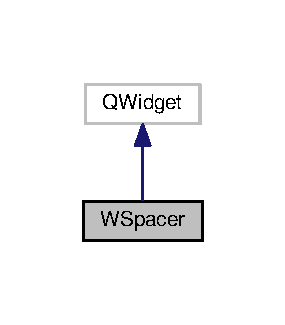
\includegraphics[width=137pt]{class_w_spacer__inherit__graph}
\end{center}
\end{figure}


Graphe de collaboration de W\+Spacer\+:\nopagebreak
\begin{figure}[H]
\begin{center}
\leavevmode
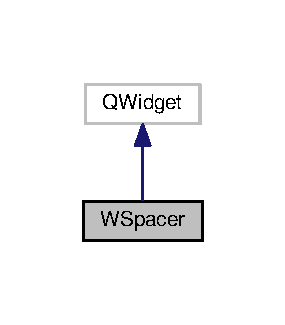
\includegraphics[width=137pt]{class_w_spacer__coll__graph}
\end{center}
\end{figure}
\subsection*{Fonctions membres publiques}
\begin{DoxyCompactItemize}
\item 
\hyperlink{class_w_spacer_a906951f82972d8433437a929ec6afd3c}{W\+Spacer} ()
\end{DoxyCompactItemize}


\subsection{Description détaillée}
hérite de Q\+Widget met un espace dans la Q\+Tool\+Bar 

\subsection{Documentation des constructeurs et destructeur}
\index{W\+Spacer@{W\+Spacer}!W\+Spacer@{W\+Spacer}}
\index{W\+Spacer@{W\+Spacer}!W\+Spacer@{W\+Spacer}}
\subsubsection[{\texorpdfstring{W\+Spacer()}{WSpacer()}}]{\setlength{\rightskip}{0pt plus 5cm}W\+Spacer\+::\+W\+Spacer (
\begin{DoxyParamCaption}
{}
\end{DoxyParamCaption}
)\hspace{0.3cm}{\ttfamily [inline]}}\hypertarget{class_w_spacer_a906951f82972d8433437a929ec6afd3c}{}\label{class_w_spacer_a906951f82972d8433437a929ec6afd3c}


La documentation de cette classe a été générée à partir du fichier suivant \+:\begin{DoxyCompactItemize}
\item 
info/\+L\+O21/\+L\+O21/\+Auto\+Cell/\hyperlink{mainwindow_8h}{mainwindow.\+h}\end{DoxyCompactItemize}

\chapter{Documentation des fichiers}
\hypertarget{autocell_8cpp}{}\section{Référence du fichier info/\+L\+O21/\+L\+O21/\+Auto\+Cell/autocell.cpp}
\label{autocell_8cpp}\index{info/\+L\+O21/\+L\+O21/\+Auto\+Cell/autocell.\+cpp@{info/\+L\+O21/\+L\+O21/\+Auto\+Cell/autocell.\+cpp}}
{\ttfamily \#include \char`\"{}autocell.\+h\char`\"{}}\\*
{\ttfamily \#include \char`\"{}Automate2\+D.\+h\char`\"{}}\\*
{\ttfamily \#include \char`\"{}Etat2\+D.\+h\char`\"{}}\\*
{\ttfamily \#include \char`\"{}Etat1\+D.\+h\char`\"{}}\\*
Graphe des dépendances par inclusion de autocell.\+cpp\+:\nopagebreak
\begin{figure}[H]
\begin{center}
\leavevmode
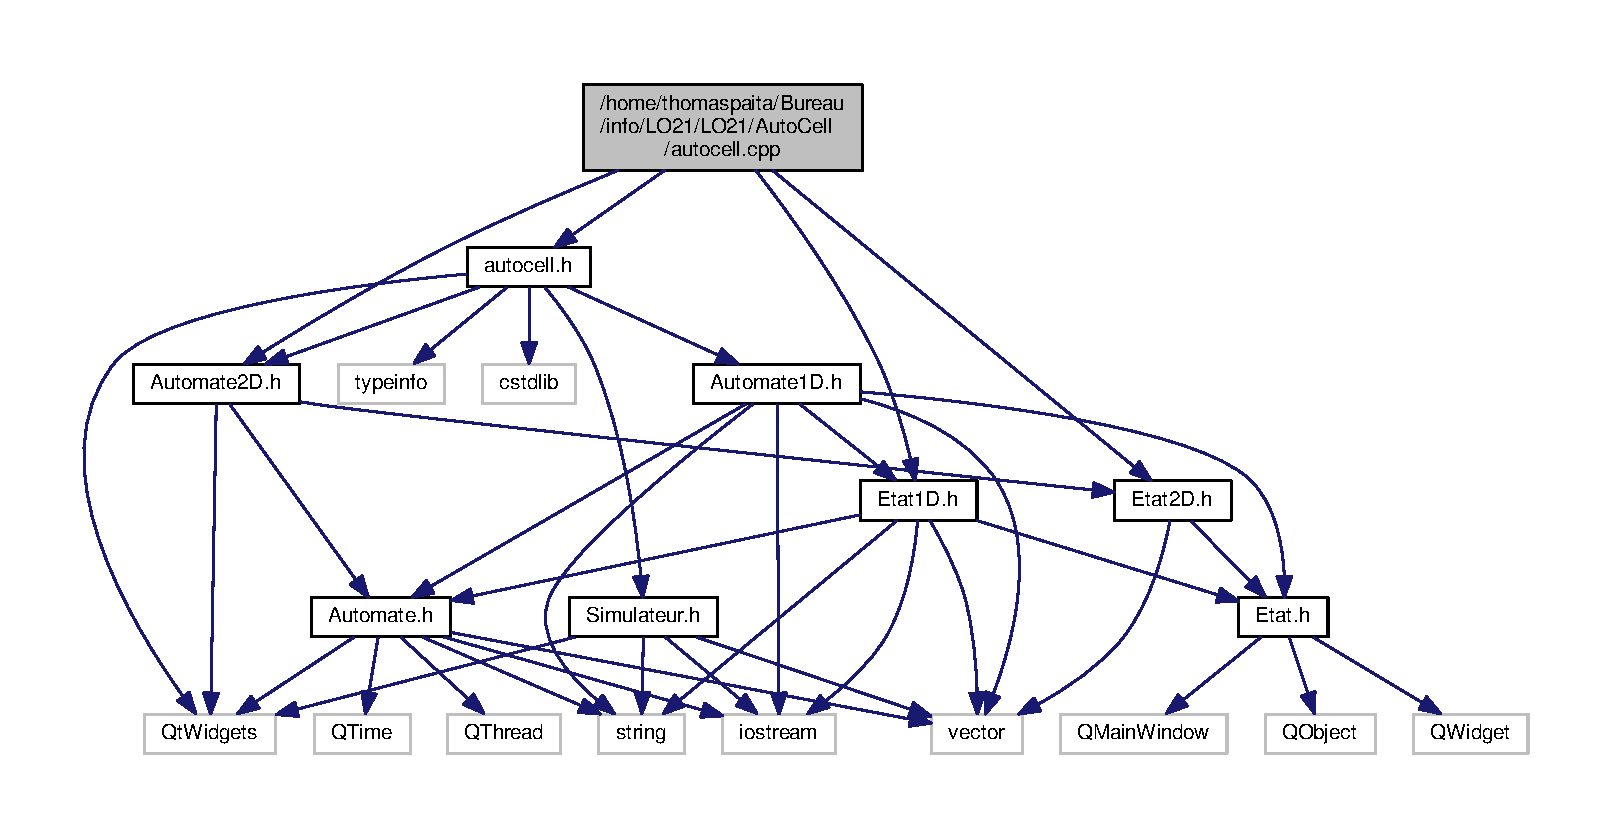
\includegraphics[width=350pt]{autocell_8cpp__incl}
\end{center}
\end{figure}
\subsection*{Fonctions}
\begin{DoxyCompactItemize}
\item 
void \hyperlink{autocell_8cpp_a884424651dc09b6a2ab852be013e4365}{delay} (int n)
\end{DoxyCompactItemize}


\subsection{Documentation des fonctions}
\index{autocell.\+cpp@{autocell.\+cpp}!delay@{delay}}
\index{delay@{delay}!autocell.\+cpp@{autocell.\+cpp}}
\subsubsection[{\texorpdfstring{delay(int n)}{delay(int n)}}]{\setlength{\rightskip}{0pt plus 5cm}void delay (
\begin{DoxyParamCaption}
\item[{int}]{n}
\end{DoxyParamCaption}
)}\hypertarget{autocell_8cpp_a884424651dc09b6a2ab852be013e4365}{}\label{autocell_8cpp_a884424651dc09b6a2ab852be013e4365}

\hypertarget{autocell_8h}{}\section{Référence du fichier /home/thomaspaita/\+Bureau/info/\+L\+O21/\+L\+O21/\+Auto\+Cell/autocell.h}
\label{autocell_8h}\index{/home/thomaspaita/\+Bureau/info/\+L\+O21/\+L\+O21/\+Auto\+Cell/autocell.\+h@{/home/thomaspaita/\+Bureau/info/\+L\+O21/\+L\+O21/\+Auto\+Cell/autocell.\+h}}


Gestion graphique des Automates cellulaires 1D et 2D.  


{\ttfamily \#include $<$Qt\+Widgets$>$}\\*
{\ttfamily \#include $<$typeinfo$>$}\\*
{\ttfamily \#include $<$cstdlib$>$}\\*
{\ttfamily \#include \char`\"{}Automate1\+D.\+h\char`\"{}}\\*
{\ttfamily \#include \char`\"{}Automate2\+D.\+h\char`\"{}}\\*
{\ttfamily \#include \char`\"{}Simulateur.\+h\char`\"{}}\\*
Graphe des dépendances par inclusion de autocell.\+h\+:
\nopagebreak
\begin{figure}[H]
\begin{center}
\leavevmode
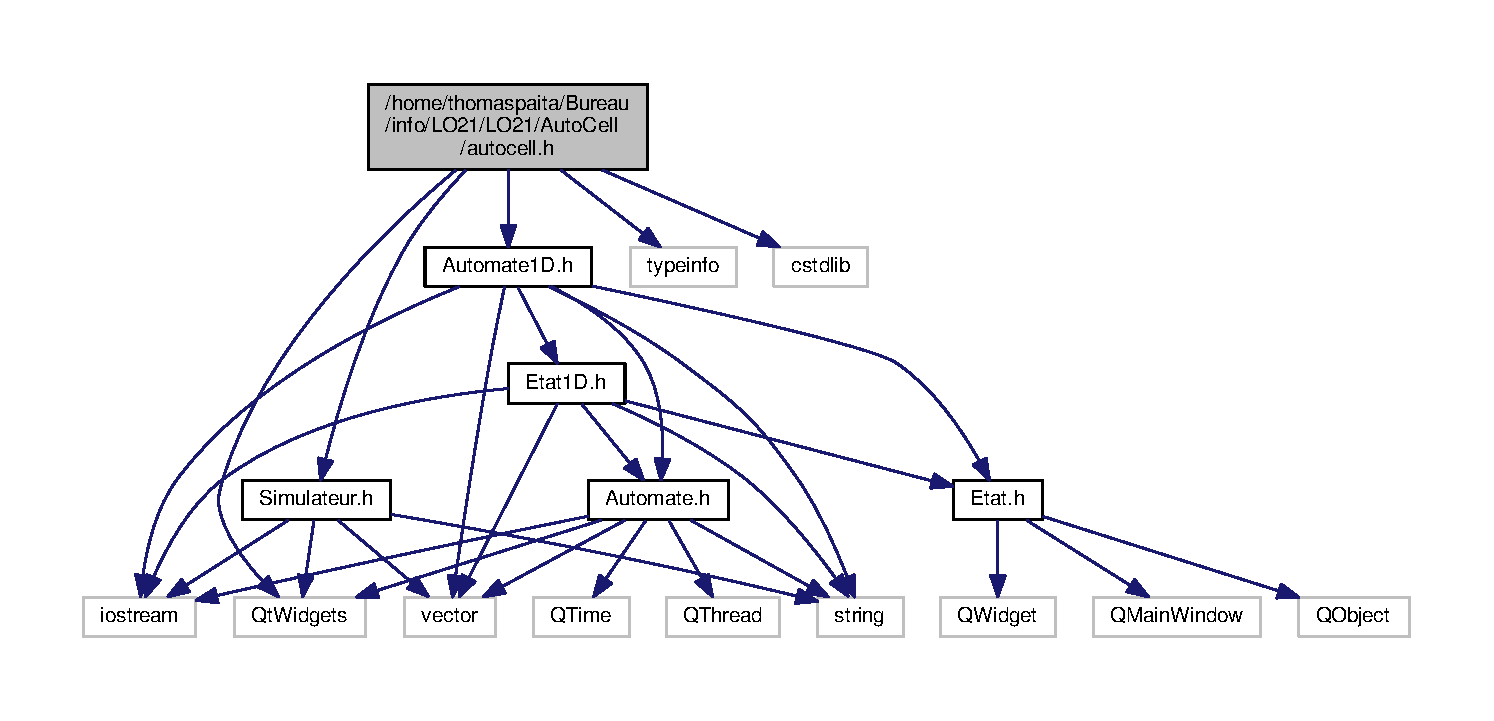
\includegraphics[width=350pt]{autocell_8h__incl}
\end{center}
\end{figure}
Ce graphe montre quels fichiers incluent directement ou indirectement ce fichier \+:\nopagebreak
\begin{figure}[H]
\begin{center}
\leavevmode
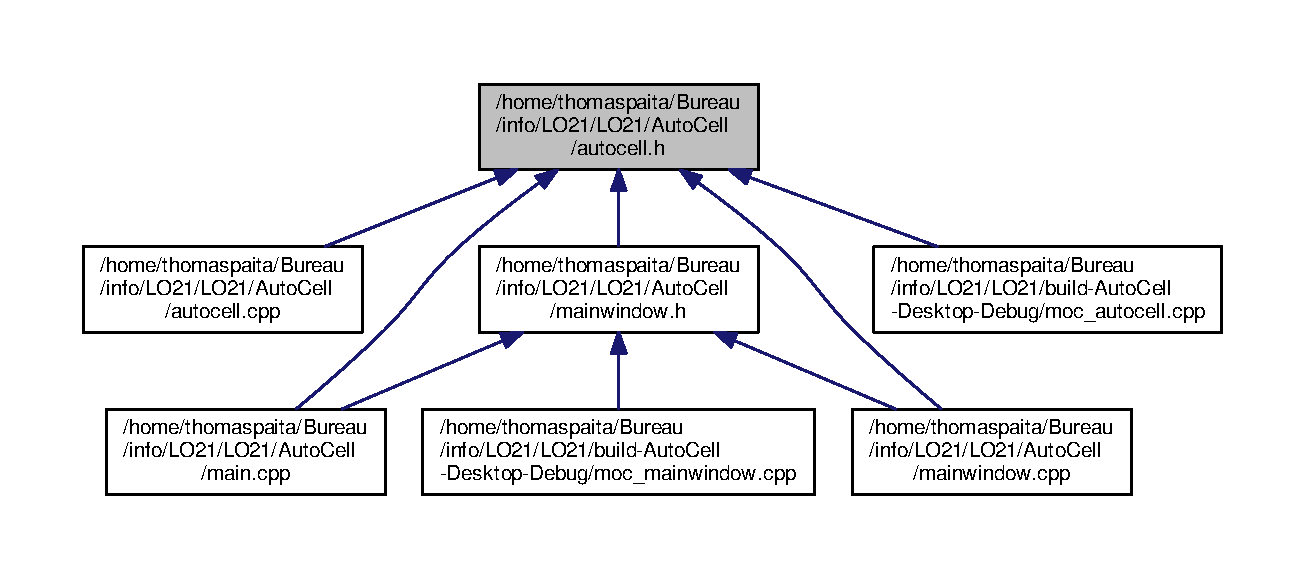
\includegraphics[width=350pt]{autocell_8h__dep__incl}
\end{center}
\end{figure}
\subsection*{Classes}
\begin{DoxyCompactItemize}
\item 
class \hyperlink{class_autocell}{Autocell}
\begin{DoxyCompactList}\small\item\em Classe abstraite. La classe généralise un \hyperlink{class_autocell}{Autocell} et définie les méthodes virtuelles qui devront être présente et définie dans chaque \hyperlink{class_autocell}{Autocell}. La fenetre principale va alors mettre en action le polymorphisme, permettant alors de lancer, arrêter... n\textquotesingle{}importe quel \hyperlink{class_autocell}{Autocell}. \end{DoxyCompactList}\item 
class \hyperlink{class_autocell1_d}{Autocell1D}
\begin{DoxyCompactList}\small\item\em Hérite de \hyperlink{class_autocell}{Autocell}. La classe \hyperlink{class_autocell1_d}{Autocell1D} permet de lancer des automates cellulaires à 1\+Dimensions (classe \hyperlink{class_automate1_d}{Automate1D} et \hyperlink{class_etat1_d}{Etat1D}) \end{DoxyCompactList}\item 
class \hyperlink{class_autocell2_d}{Autocell2D}
\begin{DoxyCompactList}\small\item\em Hérite de \hyperlink{class_autocell}{Autocell}. La classe \hyperlink{class_autocell2_d}{Autocell2D} permet de lancer des automates cellulaires à 2\+Dimensions (classe \hyperlink{class_automate2_d}{Automate2D} et \hyperlink{class_etat2_d}{Etat2D}) \end{DoxyCompactList}\item 
class \hyperlink{class_regle2_d}{Regle2D}
\begin{DoxyCompactList}\small\item\em Hérite de Q\+Widget. La classe \hyperlink{class_regle2_d}{Regle2D} permet d\textquotesingle{}entrer une règle pour un autocell2D (classe \hyperlink{class_automate2_d}{Automate2D} et \hyperlink{class_etat2_d}{Etat2D}) \end{DoxyCompactList}\item 
class \hyperlink{class_regle2_d_bis}{Regle2\+D\+Bis}
\begin{DoxyCompactList}\small\item\em Hérite de \hyperlink{class_regle2_d}{Regle2D} La classe \hyperlink{class_regle2_d_bis}{Regle2\+D\+Bis} montre comment intégrer de nouvelles règles à un autocell2D. \end{DoxyCompactList}\item 
class \hyperlink{class_autocell2_d_bis}{Autocell2\+D\+Bis}
\begin{DoxyCompactList}\small\item\em Hérite de \hyperlink{class_autocell2_d}{Autocell2D}. La classe \hyperlink{class_autocell2_d_bis}{Autocell2\+D\+Bis} montre comment intégrer de nouvelles règles à un autocell2D. \end{DoxyCompactList}\end{DoxyCompactItemize}


\subsection{Description détaillée}
Gestion graphique des Automates cellulaires 1D et 2D. 

\begin{DoxyVersion}{Version}
1.\+0 
\end{DoxyVersion}

\hypertarget{_automate_8cpp}{}\section{Référence du fichier info/\+L\+O21/\+L\+O21/\+Auto\+Cell/\+Automate.cpp}
\label{_automate_8cpp}\index{info/\+L\+O21/\+L\+O21/\+Auto\+Cell/\+Automate.\+cpp@{info/\+L\+O21/\+L\+O21/\+Auto\+Cell/\+Automate.\+cpp}}

\hypertarget{_automate_8h}{}\section{Référence du fichier /home/thomaspaita/\+Bureau/info/\+L\+O21/\+L\+O21/\+Auto\+Cell/\+Automate.h}
\label{_automate_8h}\index{/home/thomaspaita/\+Bureau/info/\+L\+O21/\+L\+O21/\+Auto\+Cell/\+Automate.\+h@{/home/thomaspaita/\+Bureau/info/\+L\+O21/\+L\+O21/\+Auto\+Cell/\+Automate.\+h}}


Structure de Base d\textquotesingle{}un \hyperlink{class_automate}{Automate}.  


{\ttfamily \#include $<$Qt\+Widgets$>$}\\*
{\ttfamily \#include $<$Q\+Thread$>$}\\*
{\ttfamily \#include $<$Q\+Time$>$}\\*
{\ttfamily \#include $<$iostream$>$}\\*
{\ttfamily \#include $<$string$>$}\\*
{\ttfamily \#include $<$vector$>$}\\*
Graphe des dépendances par inclusion de Automate.\+h\+:\nopagebreak
\begin{figure}[H]
\begin{center}
\leavevmode
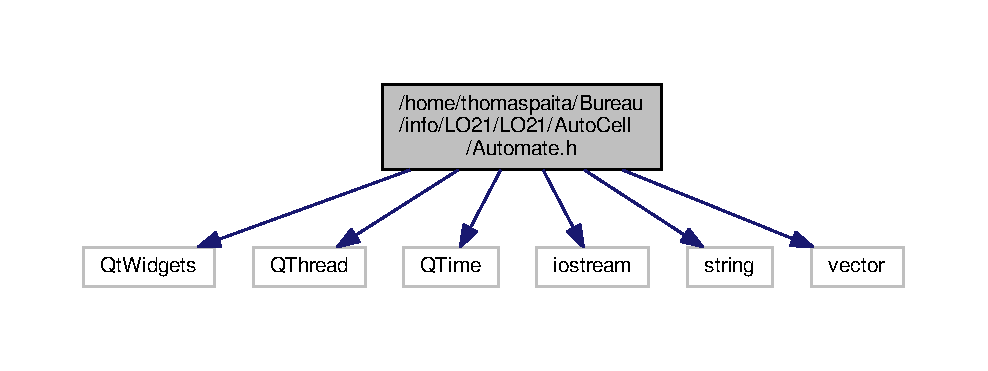
\includegraphics[width=350pt]{_automate_8h__incl}
\end{center}
\end{figure}
Ce graphe montre quels fichiers incluent directement ou indirectement ce fichier \+:\nopagebreak
\begin{figure}[H]
\begin{center}
\leavevmode
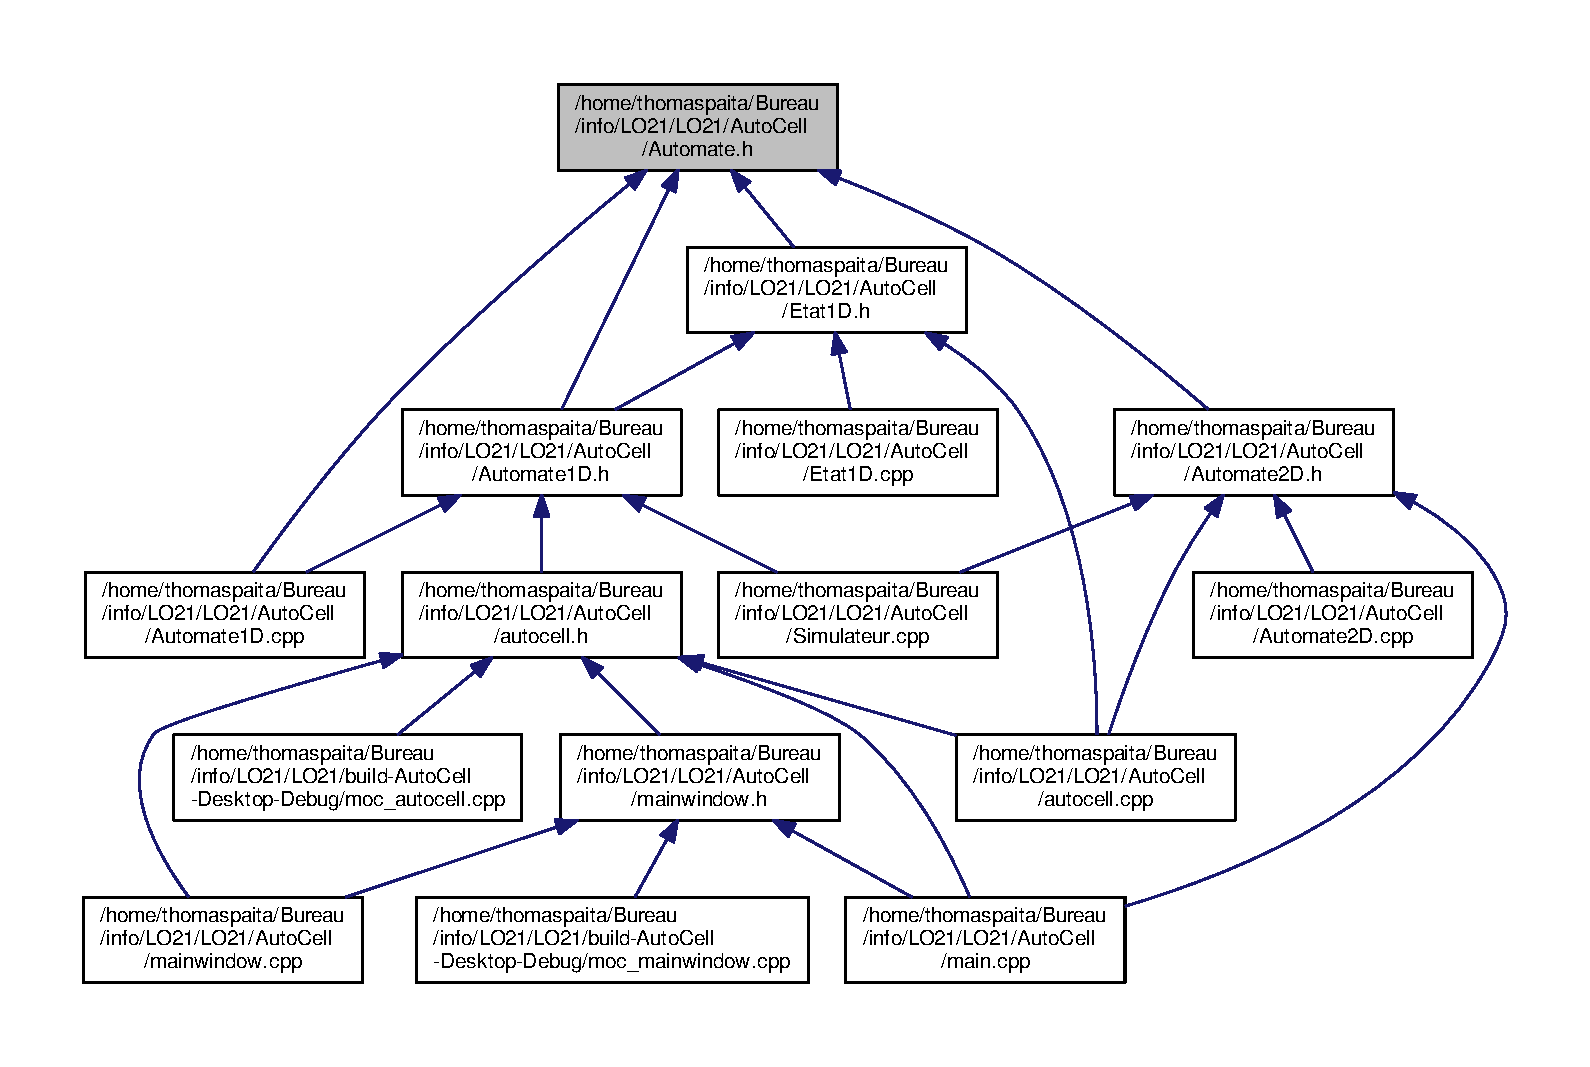
\includegraphics[width=350pt]{_automate_8h__dep__incl}
\end{center}
\end{figure}
\subsection*{Classes}
\begin{DoxyCompactItemize}
\item 
class \hyperlink{class_automate}{Automate$<$ T $>$}
\begin{DoxyCompactList}\small\item\em Classe Template abstraite. La classe généralise un \hyperlink{class_automate}{Automate} et définie la méthodes virtuelle qui devra être présente et définie dans chaque \hyperlink{class_automate}{Automate}. (run\+Sim()) \end{DoxyCompactList}\end{DoxyCompactItemize}


\subsection{Description détaillée}
Structure de Base d\textquotesingle{}un \hyperlink{class_automate}{Automate}. 

\begin{DoxyVersion}{Version}
1.\+0 
\end{DoxyVersion}

\hypertarget{_automate1_d_8cpp}{}\section{Référence du fichier info/\+L\+O21/\+L\+O21/\+Auto\+Cell/\+Automate1D.cpp}
\label{_automate1_d_8cpp}\index{info/\+L\+O21/\+L\+O21/\+Auto\+Cell/\+Automate1\+D.\+cpp@{info/\+L\+O21/\+L\+O21/\+Auto\+Cell/\+Automate1\+D.\+cpp}}
{\ttfamily \#include \char`\"{}Automate1\+D.\+h\char`\"{}}\\*
{\ttfamily \#include \char`\"{}Automate.\+h\char`\"{}}\\*
{\ttfamily \#include $<$iostream$>$}\\*
Graphe des dépendances par inclusion de Automate1\+D.\+cpp\+:\nopagebreak
\begin{figure}[H]
\begin{center}
\leavevmode
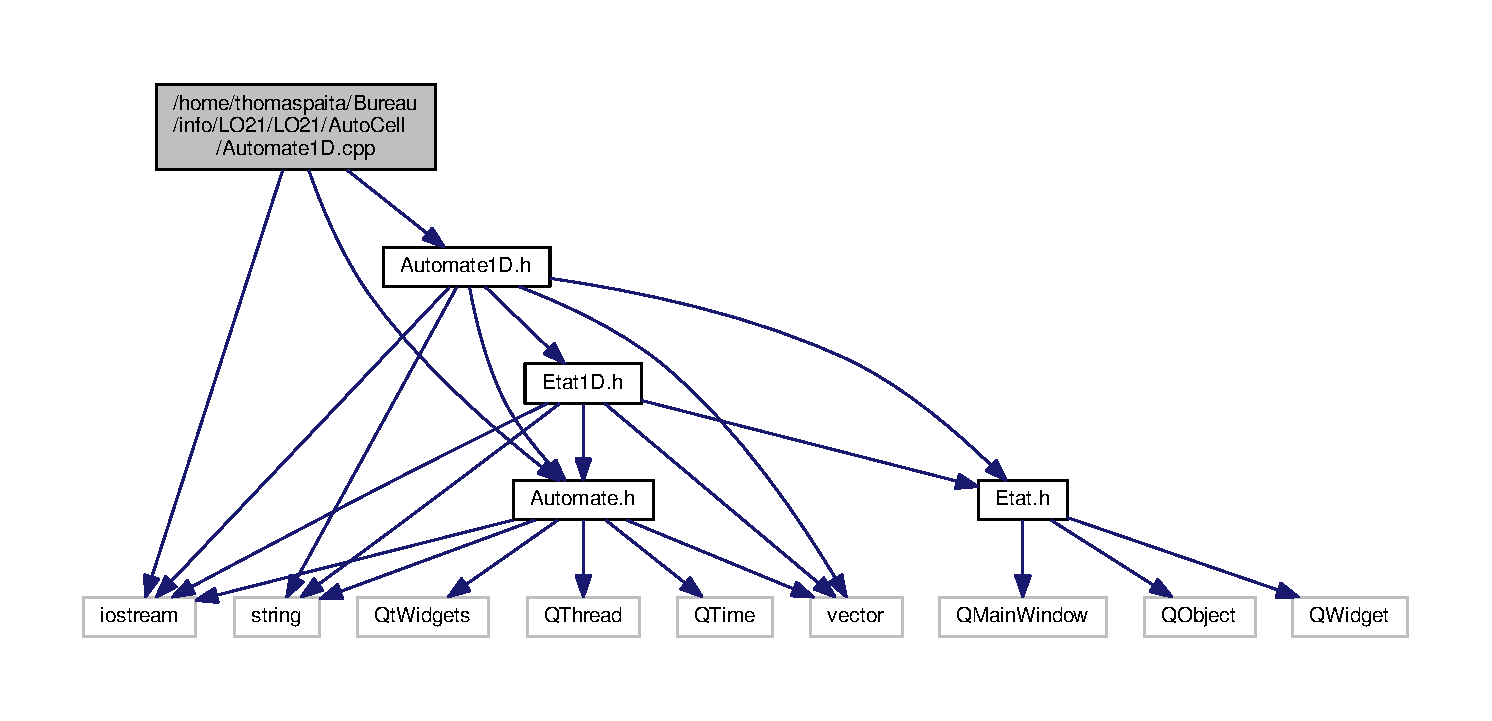
\includegraphics[width=350pt]{_automate1_d_8cpp__incl}
\end{center}
\end{figure}
\subsection*{Fonctions}
\begin{DoxyCompactItemize}
\item 
short unsigned int \hyperlink{_automate1_d_8cpp_aaefffc64e67992ad922bc54ced3e3d50}{Num\+Bit\+To\+Num} (const std\+::string \&num)
\item 
std\+::string \hyperlink{_automate1_d_8cpp_abc9c082c2b96399293dac2d8455991af}{Num\+To\+Num\+Bit} (short unsigned int num)
\item 
ostream \& \hyperlink{_automate1_d_8cpp_a27e08406c9399bba1f48138fa2dc8274}{operator$<$$<$} (ostream \&flux, const \hyperlink{class_automate1_d}{Automate1D} \&automate)
\end{DoxyCompactItemize}


\subsection{Documentation des fonctions}
\index{Automate1\+D.\+cpp@{Automate1\+D.\+cpp}!Num\+Bit\+To\+Num@{Num\+Bit\+To\+Num}}
\index{Num\+Bit\+To\+Num@{Num\+Bit\+To\+Num}!Automate1\+D.\+cpp@{Automate1\+D.\+cpp}}
\subsubsection[{\texorpdfstring{Num\+Bit\+To\+Num(const std\+::string \&num)}{NumBitToNum(const std::string &num)}}]{\setlength{\rightskip}{0pt plus 5cm}short unsigned int Num\+Bit\+To\+Num (
\begin{DoxyParamCaption}
\item[{const std\+::string \&}]{num}
\end{DoxyParamCaption}
)}\hypertarget{_automate1_d_8cpp_aaefffc64e67992ad922bc54ced3e3d50}{}\label{_automate1_d_8cpp_aaefffc64e67992ad922bc54ced3e3d50}
\index{Automate1\+D.\+cpp@{Automate1\+D.\+cpp}!Num\+To\+Num\+Bit@{Num\+To\+Num\+Bit}}
\index{Num\+To\+Num\+Bit@{Num\+To\+Num\+Bit}!Automate1\+D.\+cpp@{Automate1\+D.\+cpp}}
\subsubsection[{\texorpdfstring{Num\+To\+Num\+Bit(short unsigned int num)}{NumToNumBit(short unsigned int num)}}]{\setlength{\rightskip}{0pt plus 5cm}std\+::string Num\+To\+Num\+Bit (
\begin{DoxyParamCaption}
\item[{short unsigned int}]{num}
\end{DoxyParamCaption}
)}\hypertarget{_automate1_d_8cpp_abc9c082c2b96399293dac2d8455991af}{}\label{_automate1_d_8cpp_abc9c082c2b96399293dac2d8455991af}
\index{Automate1\+D.\+cpp@{Automate1\+D.\+cpp}!operator$<$$<$@{operator$<$$<$}}
\index{operator$<$$<$@{operator$<$$<$}!Automate1\+D.\+cpp@{Automate1\+D.\+cpp}}
\subsubsection[{\texorpdfstring{operator$<$$<$(ostream \&flux, const Automate1\+D \&automate)}{operator<<(ostream &flux, const Automate1D &automate)}}]{\setlength{\rightskip}{0pt plus 5cm}ostream\& operator$<$$<$ (
\begin{DoxyParamCaption}
\item[{ostream \&}]{flux, }
\item[{const {\bf Automate1D} \&}]{automate}
\end{DoxyParamCaption}
)}\hypertarget{_automate1_d_8cpp_a27e08406c9399bba1f48138fa2dc8274}{}\label{_automate1_d_8cpp_a27e08406c9399bba1f48138fa2dc8274}

\hypertarget{_automate1_d_8h}{}\section{Référence du fichier /home/thomaspaita/\+Bureau/info/\+L\+O21/\+L\+O21/\+Auto\+Cell/\+Automate1D.h}
\label{_automate1_d_8h}\index{/home/thomaspaita/\+Bureau/info/\+L\+O21/\+L\+O21/\+Auto\+Cell/\+Automate1\+D.\+h@{/home/thomaspaita/\+Bureau/info/\+L\+O21/\+L\+O21/\+Auto\+Cell/\+Automate1\+D.\+h}}


Implémente l\textquotesingle{}automate 1D ainsi que les Etats 1D.  


{\ttfamily \#include $<$iostream$>$}\\*
{\ttfamily \#include $<$string$>$}\\*
{\ttfamily \#include $<$vector$>$}\\*
{\ttfamily \#include \char`\"{}Automate.\+h\char`\"{}}\\*
{\ttfamily \#include \char`\"{}Etat.\+h\char`\"{}}\\*
{\ttfamily \#include \char`\"{}Etat1\+D.\+h\char`\"{}}\\*
Graphe des dépendances par inclusion de Automate1\+D.\+h\+:\nopagebreak
\begin{figure}[H]
\begin{center}
\leavevmode
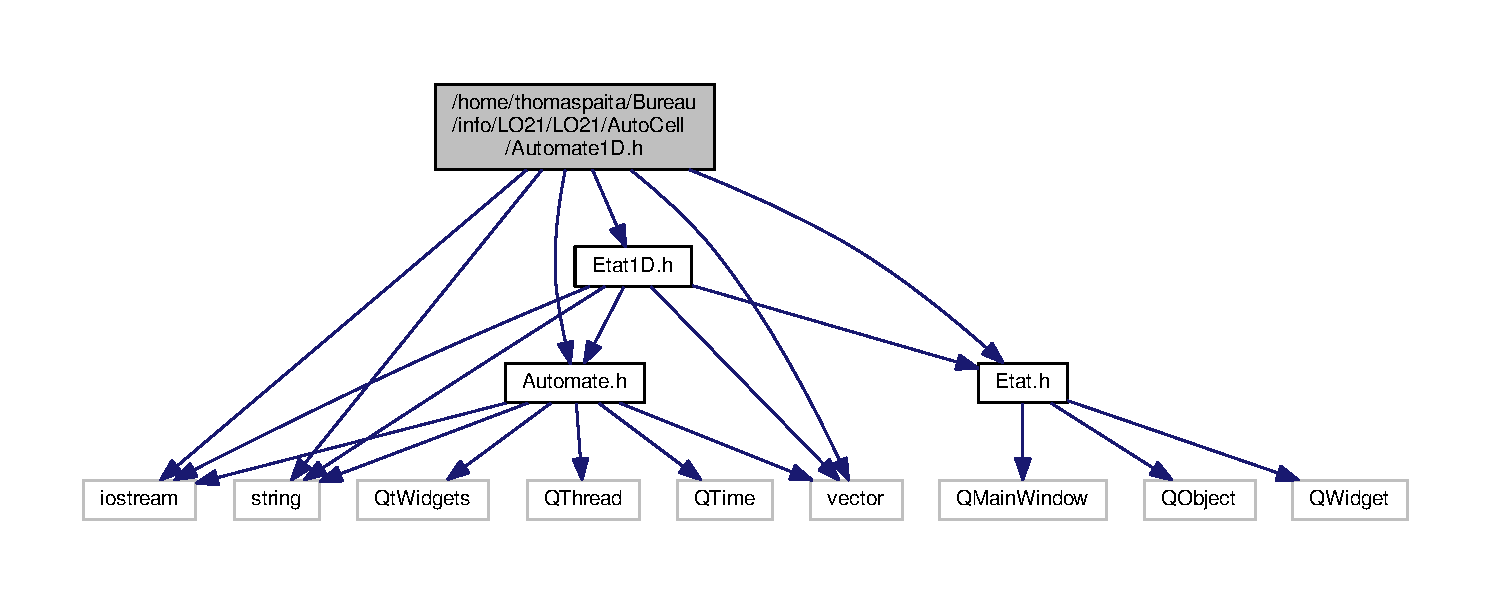
\includegraphics[width=350pt]{_automate1_d_8h__incl}
\end{center}
\end{figure}
Ce graphe montre quels fichiers incluent directement ou indirectement ce fichier \+:\nopagebreak
\begin{figure}[H]
\begin{center}
\leavevmode
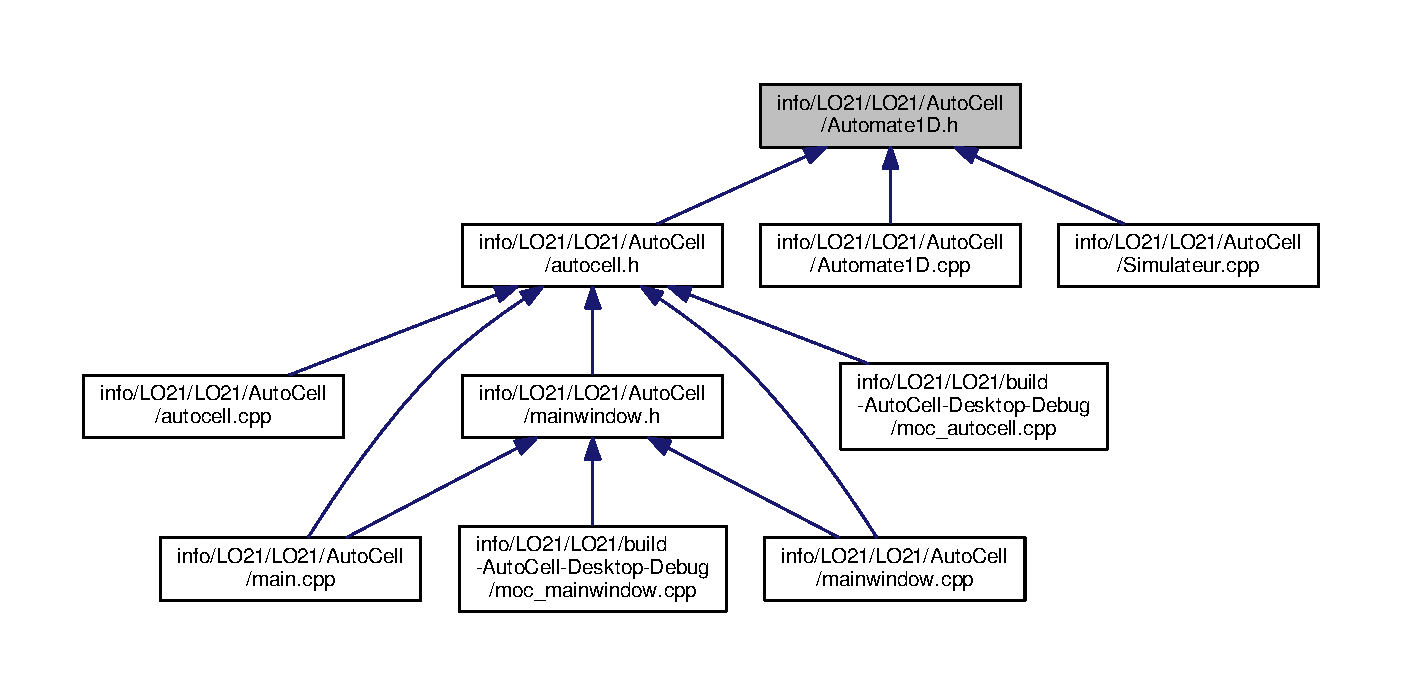
\includegraphics[width=350pt]{_automate1_d_8h__dep__incl}
\end{center}
\end{figure}
\subsection*{Classes}
\begin{DoxyCompactItemize}
\item 
class \hyperlink{class_automate}{Automate$<$ T $>$}
\begin{DoxyCompactList}\small\item\em Classe Template abstraite. La classe généralise un \hyperlink{class_automate}{Automate} et définie la méthodes virtuelle qui devra être présente et définie dans chaque \hyperlink{class_automate}{Automate}. (run\+Sim()) \end{DoxyCompactList}\item 
class \hyperlink{class_simulateur}{Simulateur$<$ T1, T2 $>$}
\begin{DoxyCompactList}\small\item\em Classe template. Permet de gérer la simulation de n\textquotesingle{}importe quel automate héritant de la Classe \hyperlink{class_automate}{Automate}. \end{DoxyCompactList}\item 
class \hyperlink{class_automate1_d}{Automate1D}
\begin{DoxyCompactList}\small\item\em hérite de \hyperlink{class_automate}{Automate$<$\+Etat1\+D$>$}. La classe permet d\textquotesingle{}appliquer une transition sur les \hyperlink{class_etat1_d}{Etat1D} suivant une règle \end{DoxyCompactList}\item 
class \hyperlink{class_automate_manager1_d}{Automate\+Manager1D}
\begin{DoxyCompactList}\small\item\em Singleton. La classe permet de gèrer la création d\textquotesingle{}automates à 1 dimension. \end{DoxyCompactList}\item 
class \hyperlink{class_automate_exception}{Automate\+Exception}
\begin{DoxyCompactList}\small\item\em permet d\textquotesingle{}envoyer des erreurs concernant les automates1D \end{DoxyCompactList}\end{DoxyCompactItemize}
\subsection*{Fonctions}
\begin{DoxyCompactItemize}
\item 
short unsigned int \hyperlink{_automate1_d_8h_aaefffc64e67992ad922bc54ced3e3d50}{Num\+Bit\+To\+Num} (const std\+::string \&num)
\item 
std\+::string \hyperlink{_automate1_d_8h_abc9c082c2b96399293dac2d8455991af}{Num\+To\+Num\+Bit} (short unsigned int num)
\item 
std\+::ostream \& \hyperlink{_automate1_d_8h_a7dc827aae58435b83f54f62f9d95840c}{operator$<$$<$} (std\+::ostream \&flux, const \hyperlink{class_etat1_d}{Etat1D} \&etat)
\item 
std\+::ostream \& \hyperlink{_automate1_d_8h_a1e5ee432e2e308d12e8e5d8d49da2aed}{operator$<$$<$} (std\+::ostream \&flux, const \hyperlink{class_automate1_d}{Automate1D} \&automate)
\end{DoxyCompactItemize}


\subsection{Description détaillée}
Implémente l\textquotesingle{}automate 1D ainsi que les Etats 1D. 

\begin{DoxyVersion}{Version}
1.\+0 
\end{DoxyVersion}


\subsection{Documentation des fonctions}
\index{Automate1\+D.\+h@{Automate1\+D.\+h}!Num\+Bit\+To\+Num@{Num\+Bit\+To\+Num}}
\index{Num\+Bit\+To\+Num@{Num\+Bit\+To\+Num}!Automate1\+D.\+h@{Automate1\+D.\+h}}
\subsubsection[{\texorpdfstring{Num\+Bit\+To\+Num(const std\+::string \&num)}{NumBitToNum(const std::string &num)}}]{\setlength{\rightskip}{0pt plus 5cm}short unsigned int Num\+Bit\+To\+Num (
\begin{DoxyParamCaption}
\item[{const std\+::string \&}]{num}
\end{DoxyParamCaption}
)}\hypertarget{_automate1_d_8h_aaefffc64e67992ad922bc54ced3e3d50}{}\label{_automate1_d_8h_aaefffc64e67992ad922bc54ced3e3d50}
\index{Automate1\+D.\+h@{Automate1\+D.\+h}!Num\+To\+Num\+Bit@{Num\+To\+Num\+Bit}}
\index{Num\+To\+Num\+Bit@{Num\+To\+Num\+Bit}!Automate1\+D.\+h@{Automate1\+D.\+h}}
\subsubsection[{\texorpdfstring{Num\+To\+Num\+Bit(short unsigned int num)}{NumToNumBit(short unsigned int num)}}]{\setlength{\rightskip}{0pt plus 5cm}std\+::string Num\+To\+Num\+Bit (
\begin{DoxyParamCaption}
\item[{short unsigned int}]{num}
\end{DoxyParamCaption}
)}\hypertarget{_automate1_d_8h_abc9c082c2b96399293dac2d8455991af}{}\label{_automate1_d_8h_abc9c082c2b96399293dac2d8455991af}
\index{Automate1\+D.\+h@{Automate1\+D.\+h}!operator$<$$<$@{operator$<$$<$}}
\index{operator$<$$<$@{operator$<$$<$}!Automate1\+D.\+h@{Automate1\+D.\+h}}
\subsubsection[{\texorpdfstring{operator$<$$<$(std\+::ostream \&flux, const Etat1\+D \&etat)}{operator<<(std::ostream &flux, const Etat1D &etat)}}]{\setlength{\rightskip}{0pt plus 5cm}std\+::ostream\& operator$<$$<$ (
\begin{DoxyParamCaption}
\item[{std\+::ostream \&}]{flux, }
\item[{const {\bf Etat1D} \&}]{etat}
\end{DoxyParamCaption}
)}\hypertarget{_automate1_d_8h_a7dc827aae58435b83f54f62f9d95840c}{}\label{_automate1_d_8h_a7dc827aae58435b83f54f62f9d95840c}
\index{Automate1\+D.\+h@{Automate1\+D.\+h}!operator$<$$<$@{operator$<$$<$}}
\index{operator$<$$<$@{operator$<$$<$}!Automate1\+D.\+h@{Automate1\+D.\+h}}
\subsubsection[{\texorpdfstring{operator$<$$<$(std\+::ostream \&flux, const Automate1\+D \&automate)}{operator<<(std::ostream &flux, const Automate1D &automate)}}]{\setlength{\rightskip}{0pt plus 5cm}std\+::ostream\& operator$<$$<$ (
\begin{DoxyParamCaption}
\item[{std\+::ostream \&}]{flux, }
\item[{const {\bf Automate1D} \&}]{automate}
\end{DoxyParamCaption}
)}\hypertarget{_automate1_d_8h_a1e5ee432e2e308d12e8e5d8d49da2aed}{}\label{_automate1_d_8h_a1e5ee432e2e308d12e8e5d8d49da2aed}

\hypertarget{_automate2_d_8cpp}{}\section{Référence du fichier info/\+L\+O21/\+L\+O21/\+Auto\+Cell/\+Automate2D.cpp}
\label{_automate2_d_8cpp}\index{info/\+L\+O21/\+L\+O21/\+Auto\+Cell/\+Automate2\+D.\+cpp@{info/\+L\+O21/\+L\+O21/\+Auto\+Cell/\+Automate2\+D.\+cpp}}
{\ttfamily \#include \char`\"{}Automate2\+D.\+h\char`\"{}}\\*
{\ttfamily \#include $<$iostream$>$}\\*
Graphe des dépendances par inclusion de Automate2\+D.\+cpp\+:\nopagebreak
\begin{figure}[H]
\begin{center}
\leavevmode
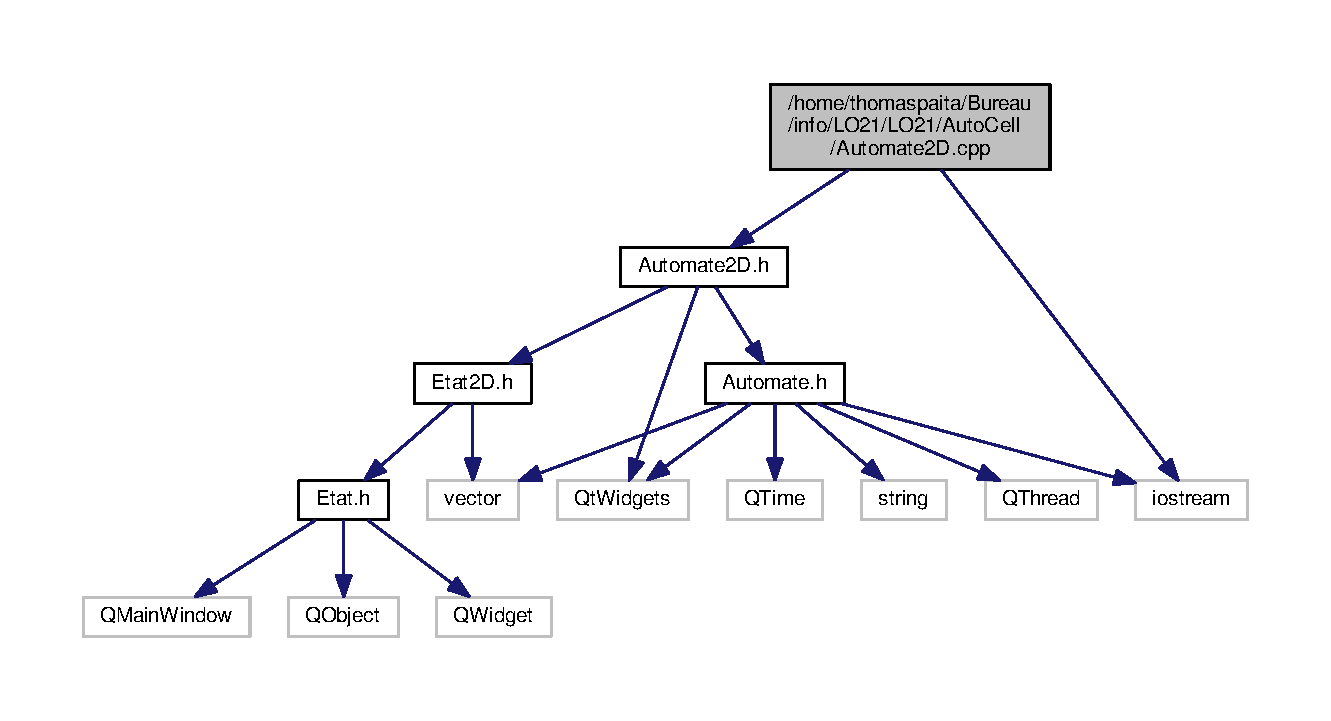
\includegraphics[width=350pt]{_automate2_d_8cpp__incl}
\end{center}
\end{figure}

\hypertarget{_automate2_d_8h}{}\section{Référence du fichier /home/thomaspaita/\+Bureau/info/\+L\+O21/\+L\+O21/\+Auto\+Cell/\+Automate2D.h}
\label{_automate2_d_8h}\index{/home/thomaspaita/\+Bureau/info/\+L\+O21/\+L\+O21/\+Auto\+Cell/\+Automate2\+D.\+h@{/home/thomaspaita/\+Bureau/info/\+L\+O21/\+L\+O21/\+Auto\+Cell/\+Automate2\+D.\+h}}


Implémente l\textquotesingle{}automate 2D ainsi que les Etats 2D.  


{\ttfamily \#include $<$Qt\+Widgets$>$}\\*
{\ttfamily \#include \char`\"{}Automate.\+h\char`\"{}}\\*
{\ttfamily \#include \char`\"{}Etat2\+D.\+h\char`\"{}}\\*
Graphe des dépendances par inclusion de Automate2\+D.\+h\+:
\nopagebreak
\begin{figure}[H]
\begin{center}
\leavevmode
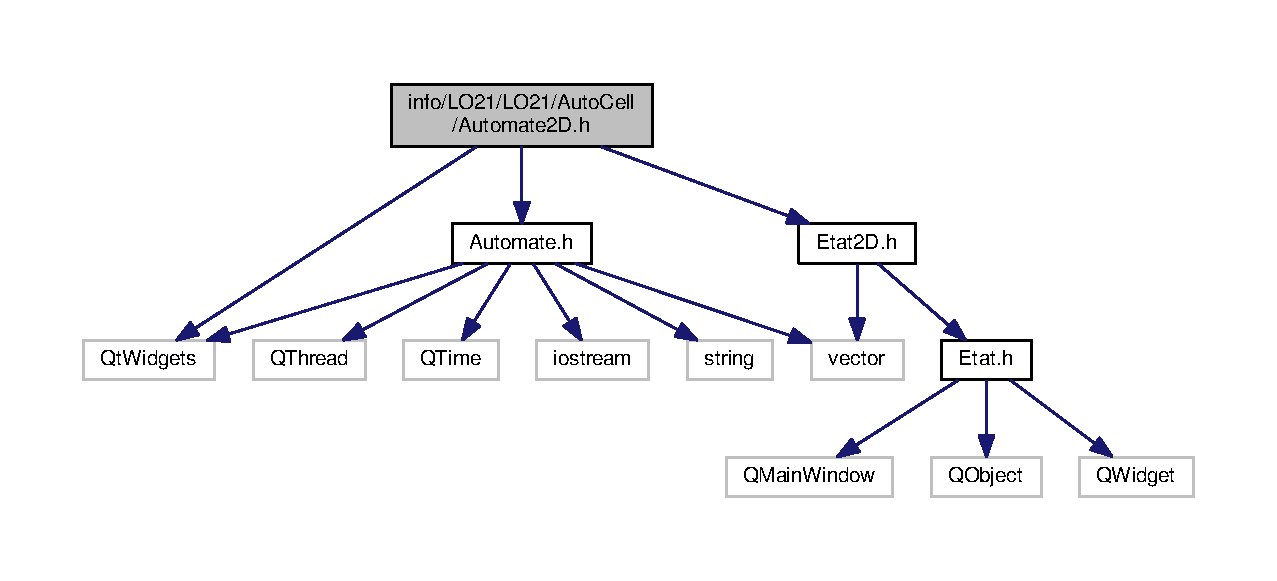
\includegraphics[width=350pt]{_automate2_d_8h__incl}
\end{center}
\end{figure}
Ce graphe montre quels fichiers incluent directement ou indirectement ce fichier \+:
\nopagebreak
\begin{figure}[H]
\begin{center}
\leavevmode
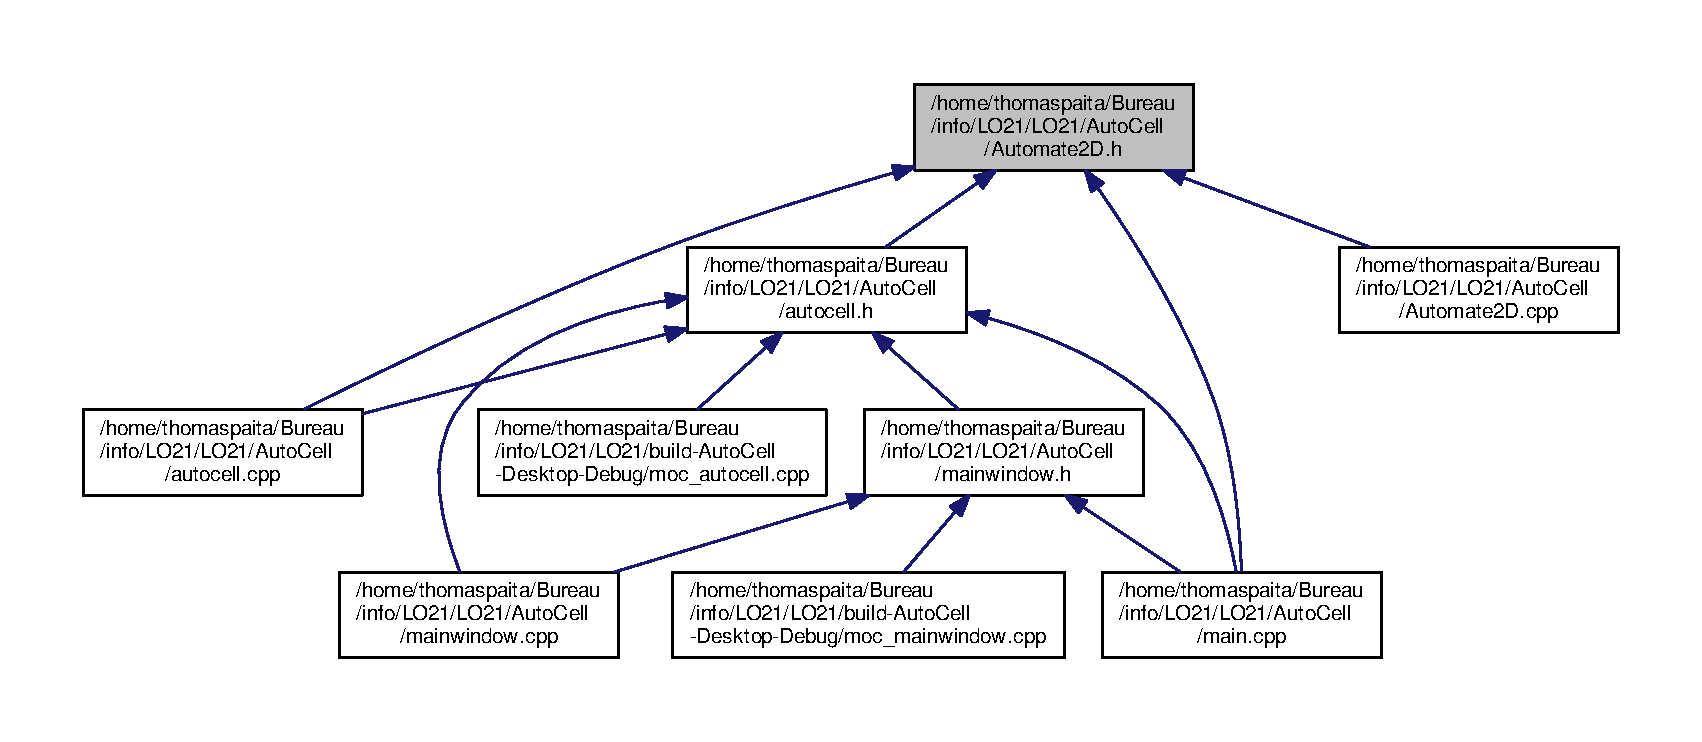
\includegraphics[width=350pt]{_automate2_d_8h__dep__incl}
\end{center}
\end{figure}
\subsection*{Classes}
\begin{DoxyCompactItemize}
\item 
class \hyperlink{class_automate2_d}{Automate2D}
\begin{DoxyCompactList}\small\item\em hérite de \hyperlink{class_automate}{Automate$<$\+Etat2\+D$>$}. La classe permet d\textquotesingle{}appliquer une transition sur les \hyperlink{class_etat2_d}{Etat2D} en suivant des règles \end{DoxyCompactList}\item 
class \hyperlink{class_automate_manager2_d}{Automate\+Manager2D}
\begin{DoxyCompactList}\small\item\em Singleton. La classe permet de gèrer la création d\textquotesingle{}automates à 2 dimensions. \end{DoxyCompactList}\end{DoxyCompactItemize}


\subsection{Description détaillée}
Implémente l\textquotesingle{}automate 2D ainsi que les Etats 2D. 

\begin{DoxyVersion}{Version}
1.\+0 
\end{DoxyVersion}

\hypertarget{_etat_8cpp}{}\section{Référence du fichier /home/thomaspaita/\+Bureau/info/\+L\+O21/\+L\+O21/\+Auto\+Cell/\+Etat.cpp}
\label{_etat_8cpp}\index{/home/thomaspaita/\+Bureau/info/\+L\+O21/\+L\+O21/\+Auto\+Cell/\+Etat.\+cpp@{/home/thomaspaita/\+Bureau/info/\+L\+O21/\+L\+O21/\+Auto\+Cell/\+Etat.\+cpp}}
{\ttfamily \#include \char`\"{}Etat.\+h\char`\"{}}\\*
Graphe des dépendances par inclusion de Etat.\+cpp\+:
\nopagebreak
\begin{figure}[H]
\begin{center}
\leavevmode
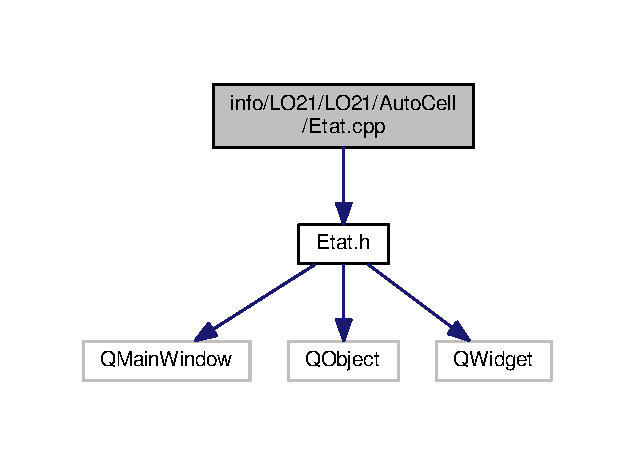
\includegraphics[width=305pt]{_etat_8cpp__incl}
\end{center}
\end{figure}

\hypertarget{_etat_8h}{}\section{Référence du fichier info/\+L\+O21/\+L\+O21/\+Auto\+Cell/\+Etat.h}
\label{_etat_8h}\index{info/\+L\+O21/\+L\+O21/\+Auto\+Cell/\+Etat.\+h@{info/\+L\+O21/\+L\+O21/\+Auto\+Cell/\+Etat.\+h}}


Permet de généraliser un \hyperlink{class_etat}{Etat}.  


{\ttfamily \#include $<$Q\+Main\+Window$>$}\\*
{\ttfamily \#include $<$Q\+Object$>$}\\*
{\ttfamily \#include $<$Q\+Widget$>$}\\*
Graphe des dépendances par inclusion de Etat.\+h\+:\nopagebreak
\begin{figure}[H]
\begin{center}
\leavevmode
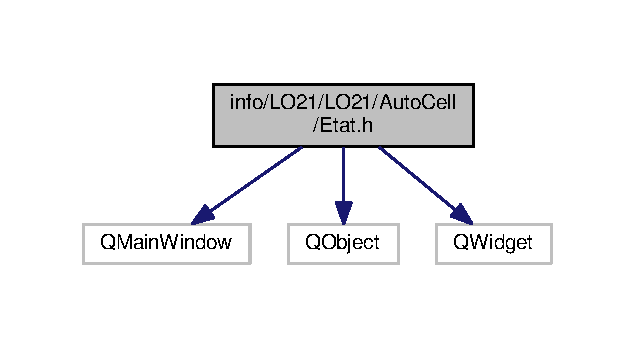
\includegraphics[width=305pt]{_etat_8h__incl}
\end{center}
\end{figure}
Ce graphe montre quels fichiers incluent directement ou indirectement ce fichier \+:\nopagebreak
\begin{figure}[H]
\begin{center}
\leavevmode
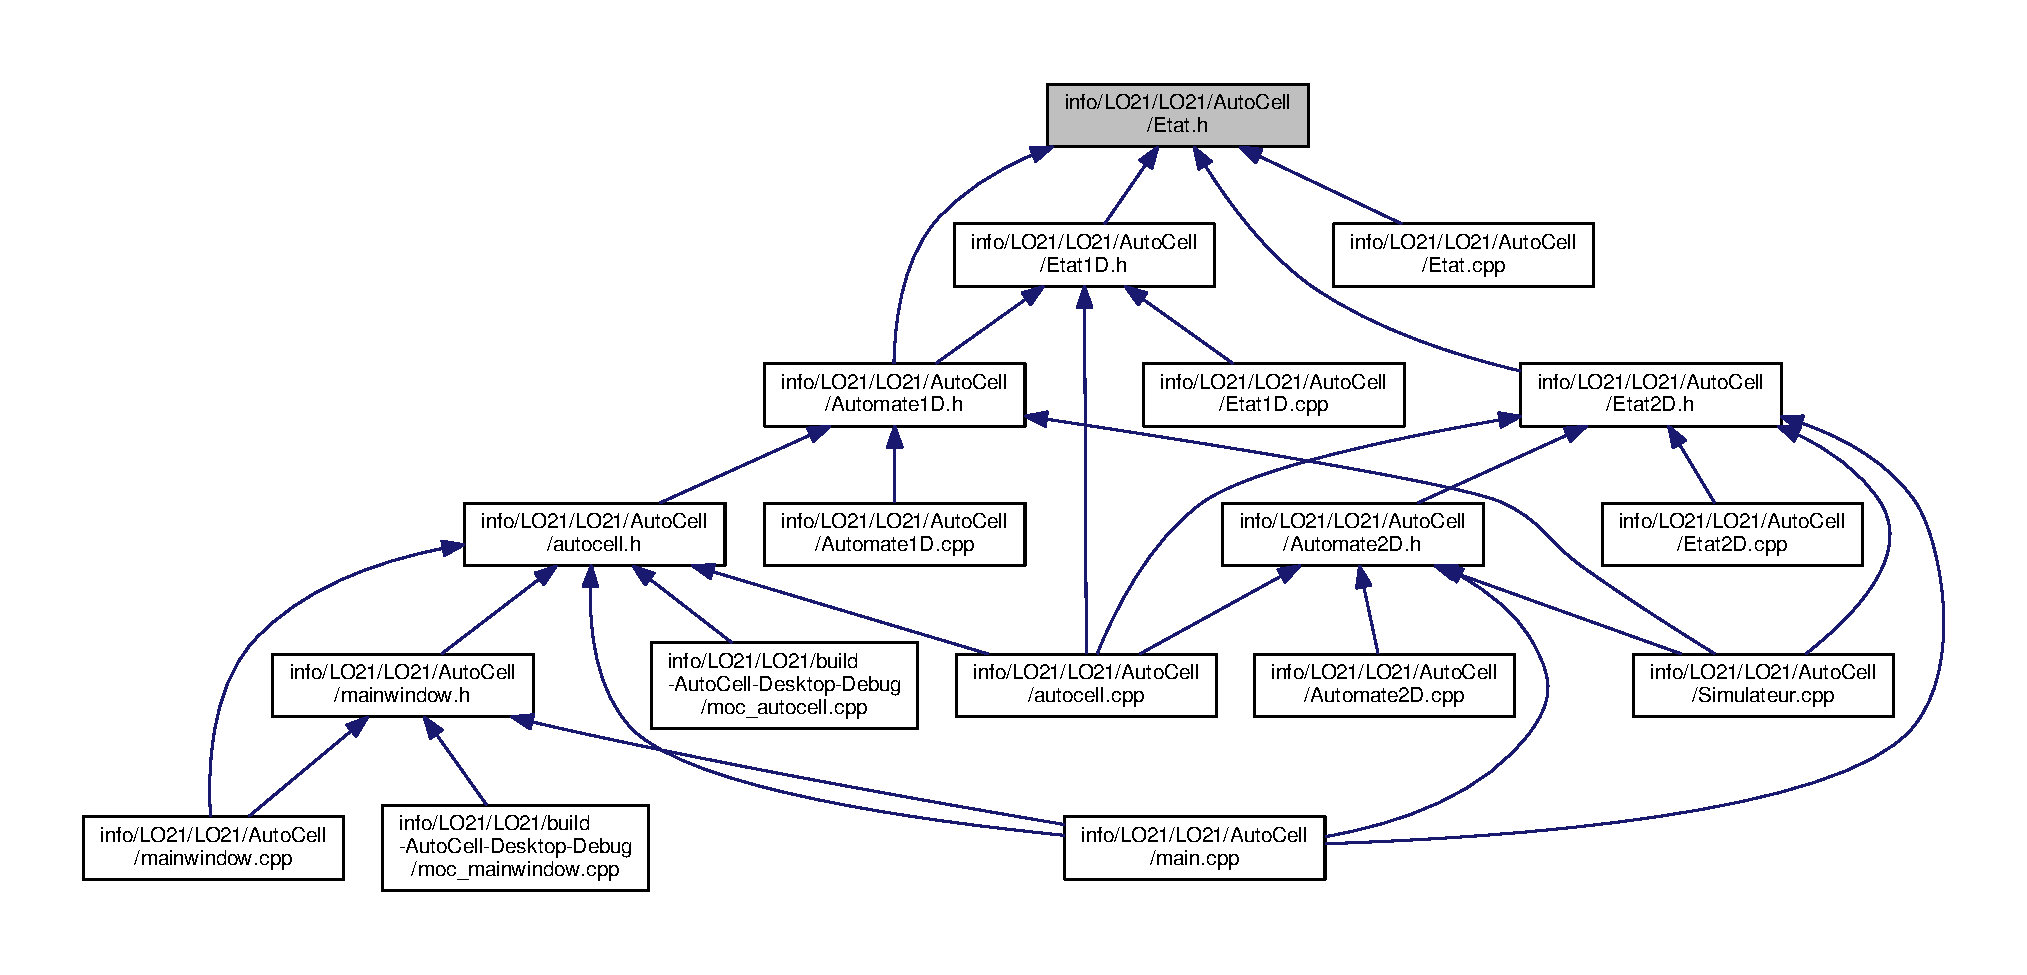
\includegraphics[width=350pt]{_etat_8h__dep__incl}
\end{center}
\end{figure}
\subsection*{Classes}
\begin{DoxyCompactItemize}
\item 
class \hyperlink{class_etat}{Etat}
\begin{DoxyCompactList}\small\item\em Classe abstraite. \end{DoxyCompactList}\end{DoxyCompactItemize}


\subsection{Description détaillée}
Permet de généraliser un \hyperlink{class_etat}{Etat}. 

\begin{DoxyVersion}{Version}
1.\+0 
\end{DoxyVersion}

\hypertarget{_etat1_d_8cpp}{}\section{Référence du fichier /home/thomaspaita/\+Bureau/info/\+L\+O21/\+L\+O21/\+Auto\+Cell/\+Etat1D.cpp}
\label{_etat1_d_8cpp}\index{/home/thomaspaita/\+Bureau/info/\+L\+O21/\+L\+O21/\+Auto\+Cell/\+Etat1\+D.\+cpp@{/home/thomaspaita/\+Bureau/info/\+L\+O21/\+L\+O21/\+Auto\+Cell/\+Etat1\+D.\+cpp}}
{\ttfamily \#include \char`\"{}Etat1\+D.\+h\char`\"{}}\\*
Graphe des dépendances par inclusion de Etat1\+D.\+cpp\+:
\nopagebreak
\begin{figure}[H]
\begin{center}
\leavevmode
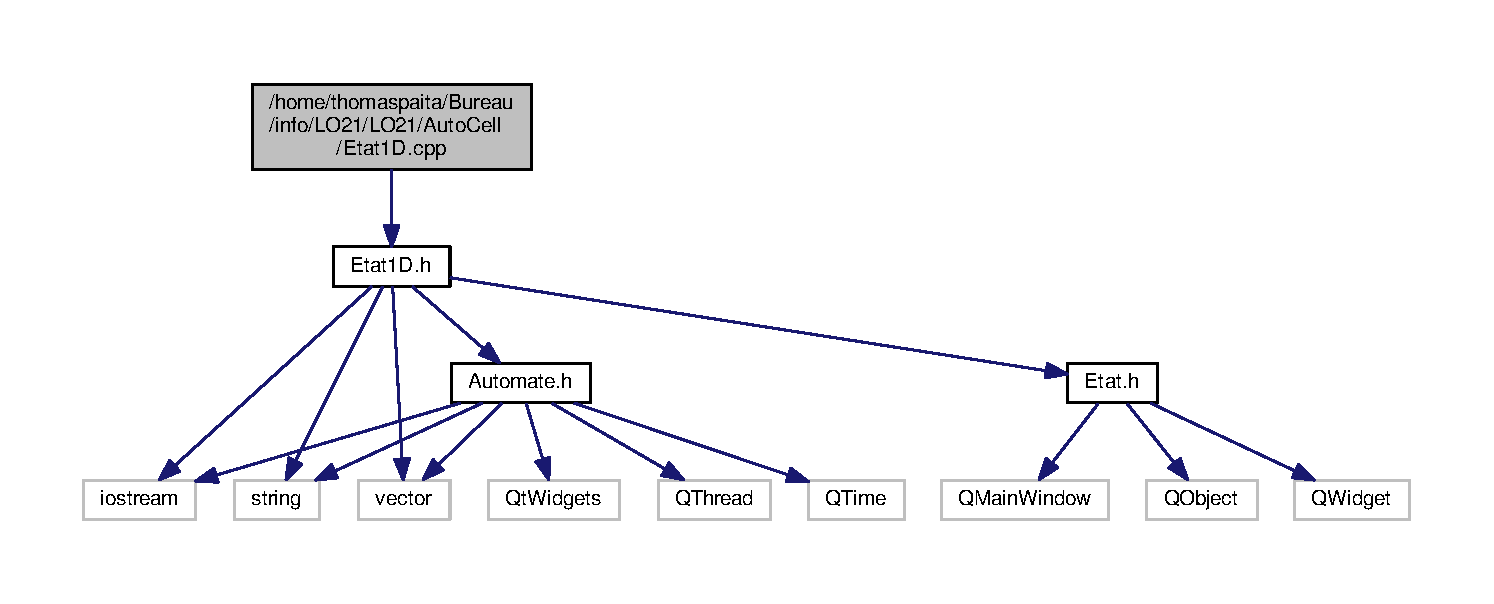
\includegraphics[width=350pt]{_etat1_d_8cpp__incl}
\end{center}
\end{figure}
\subsection*{Fonctions}
\begin{DoxyCompactItemize}
\item 
ostream \& \hyperlink{_etat1_d_8cpp_ac846718e8afab2c5299094fa71d90f2e}{operator$<$$<$} (ostream \&flux, const \hyperlink{class_etat1_d}{Etat1D} \&etat)
\end{DoxyCompactItemize}


\subsection{Documentation des fonctions}
\index{Etat1\+D.\+cpp@{Etat1\+D.\+cpp}!operator$<$$<$@{operator$<$$<$}}
\index{operator$<$$<$@{operator$<$$<$}!Etat1\+D.\+cpp@{Etat1\+D.\+cpp}}
\subsubsection[{\texorpdfstring{operator$<$$<$(ostream \&flux, const Etat1\+D \&etat)}{operator<<(ostream &flux, const Etat1D &etat)}}]{\setlength{\rightskip}{0pt plus 5cm}ostream\& operator$<$$<$ (
\begin{DoxyParamCaption}
\item[{ostream \&}]{flux, }
\item[{const {\bf Etat1D} \&}]{etat}
\end{DoxyParamCaption}
)}\hypertarget{_etat1_d_8cpp_ac846718e8afab2c5299094fa71d90f2e}{}\label{_etat1_d_8cpp_ac846718e8afab2c5299094fa71d90f2e}

\hypertarget{_etat1_d_8h}{}\section{Référence du fichier /home/thomaspaita/\+Bureau/info/\+L\+O21/\+L\+O21/\+Auto\+Cell/\+Etat1D.h}
\label{_etat1_d_8h}\index{/home/thomaspaita/\+Bureau/info/\+L\+O21/\+L\+O21/\+Auto\+Cell/\+Etat1\+D.\+h@{/home/thomaspaita/\+Bureau/info/\+L\+O21/\+L\+O21/\+Auto\+Cell/\+Etat1\+D.\+h}}


Classe pour représenter un état à 1 dimensions.  


{\ttfamily \#include $<$iostream$>$}\\*
{\ttfamily \#include $<$string$>$}\\*
{\ttfamily \#include $<$vector$>$}\\*
{\ttfamily \#include \char`\"{}Automate.\+h\char`\"{}}\\*
{\ttfamily \#include \char`\"{}Etat.\+h\char`\"{}}\\*
Graphe des dépendances par inclusion de Etat1\+D.\+h\+:\nopagebreak
\begin{figure}[H]
\begin{center}
\leavevmode
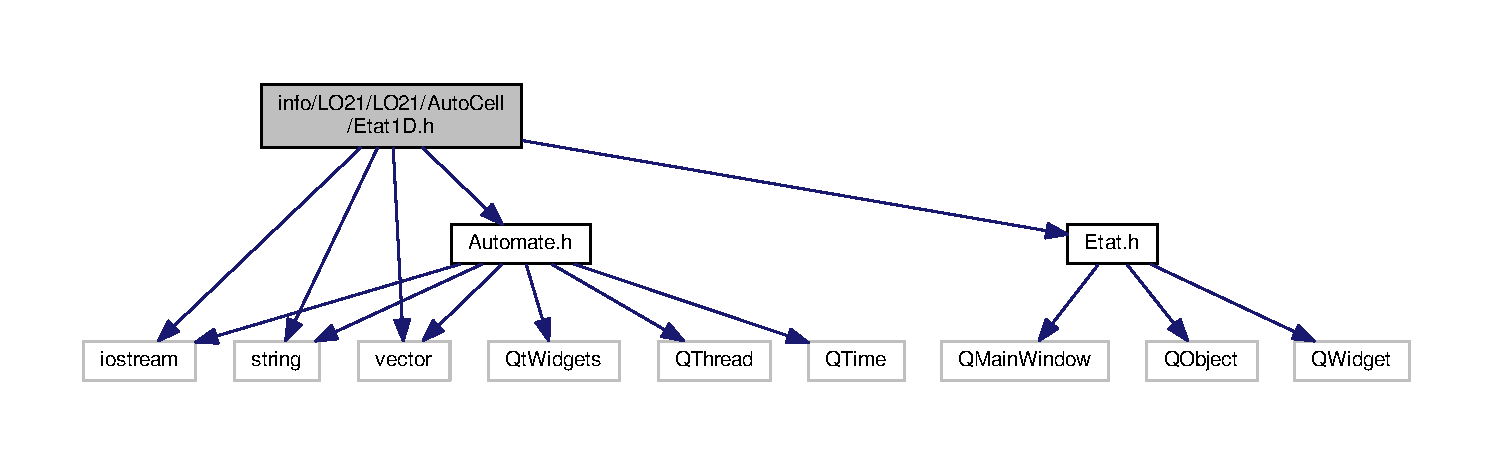
\includegraphics[width=350pt]{_etat1_d_8h__incl}
\end{center}
\end{figure}
Ce graphe montre quels fichiers incluent directement ou indirectement ce fichier \+:
\nopagebreak
\begin{figure}[H]
\begin{center}
\leavevmode
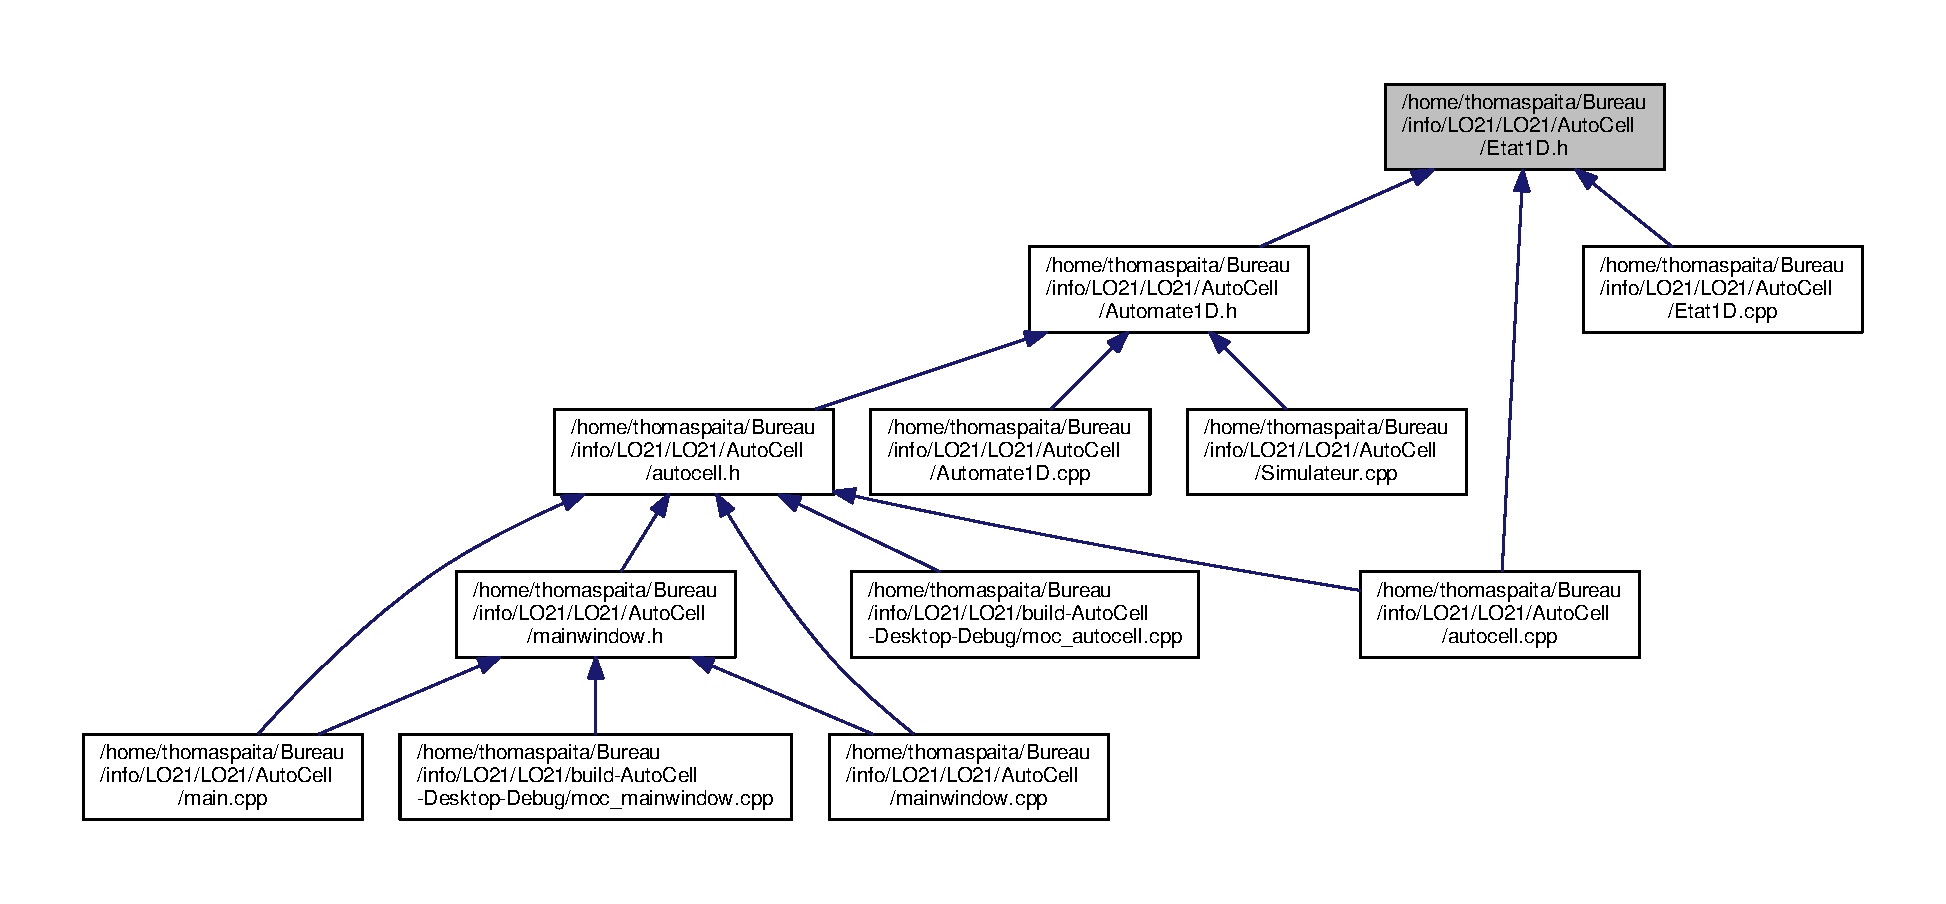
\includegraphics[width=350pt]{_etat1_d_8h__dep__incl}
\end{center}
\end{figure}
\subsection*{Classes}
\begin{DoxyCompactItemize}
\item 
class \hyperlink{class_etat1_d}{Etat1D}
\begin{DoxyCompactList}\small\item\em hérite de \hyperlink{class_etat}{Etat}. Permet de créer de état à 1\+Dimension \end{DoxyCompactList}\end{DoxyCompactItemize}


\subsection{Description détaillée}
Classe pour représenter un état à 1 dimensions. 

\begin{DoxyVersion}{Version}
1.\+0 
\end{DoxyVersion}

\hypertarget{_etat2_d_8cpp}{}\section{Référence du fichier info/\+L\+O21/\+L\+O21/\+Auto\+Cell/\+Etat2D.cpp}
\label{_etat2_d_8cpp}\index{info/\+L\+O21/\+L\+O21/\+Auto\+Cell/\+Etat2\+D.\+cpp@{info/\+L\+O21/\+L\+O21/\+Auto\+Cell/\+Etat2\+D.\+cpp}}
{\ttfamily \#include \char`\"{}Etat2\+D.\+h\char`\"{}}\\*
{\ttfamily \#include $<$iostream$>$}\\*
Graphe des dépendances par inclusion de Etat2\+D.\+cpp\+:\nopagebreak
\begin{figure}[H]
\begin{center}
\leavevmode
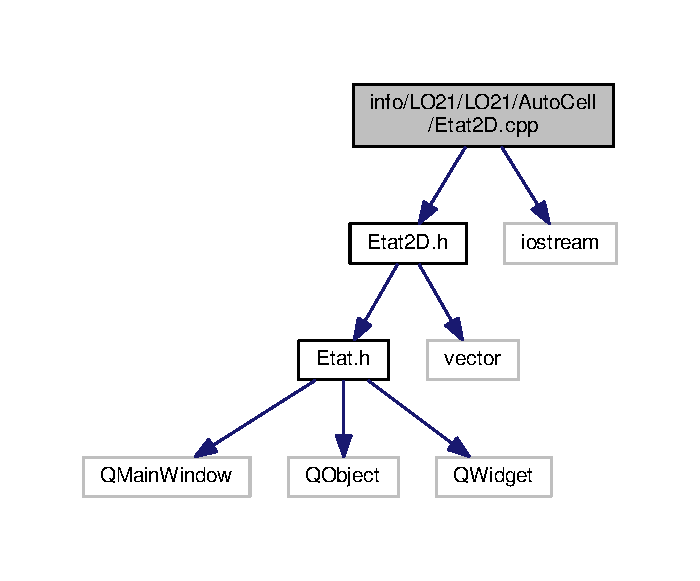
\includegraphics[width=336pt]{_etat2_d_8cpp__incl}
\end{center}
\end{figure}

\hypertarget{_etat2_d_8h}{}\section{Référence du fichier /home/thomaspaita/\+Bureau/info/\+L\+O21/\+L\+O21/\+Auto\+Cell/\+Etat2D.h}
\label{_etat2_d_8h}\index{/home/thomaspaita/\+Bureau/info/\+L\+O21/\+L\+O21/\+Auto\+Cell/\+Etat2\+D.\+h@{/home/thomaspaita/\+Bureau/info/\+L\+O21/\+L\+O21/\+Auto\+Cell/\+Etat2\+D.\+h}}


Classe pour représenter un état à 2 dimensions.  


{\ttfamily \#include \char`\"{}Etat.\+h\char`\"{}}\\*
{\ttfamily \#include $<$vector$>$}\\*
Graphe des dépendances par inclusion de Etat2\+D.\+h\+:
\nopagebreak
\begin{figure}[H]
\begin{center}
\leavevmode
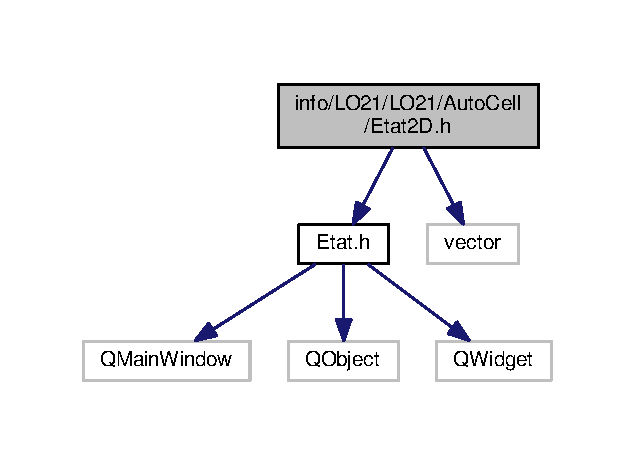
\includegraphics[width=305pt]{_etat2_d_8h__incl}
\end{center}
\end{figure}
Ce graphe montre quels fichiers incluent directement ou indirectement ce fichier \+:
\nopagebreak
\begin{figure}[H]
\begin{center}
\leavevmode
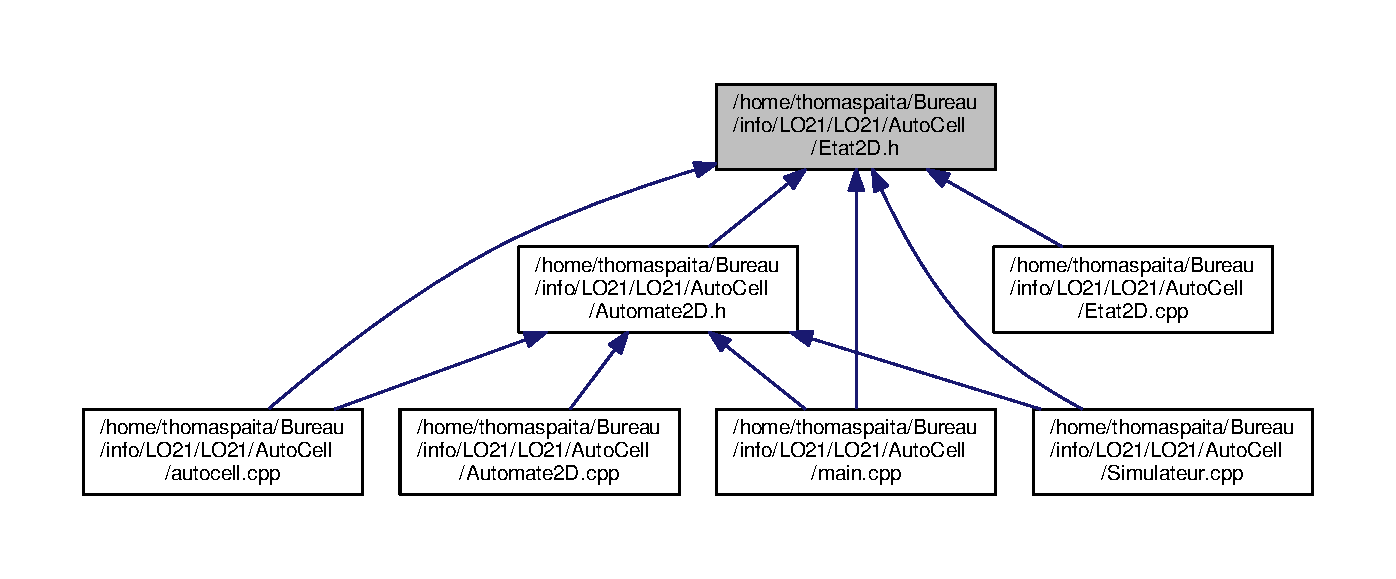
\includegraphics[width=350pt]{_etat2_d_8h__dep__incl}
\end{center}
\end{figure}
\subsection*{Classes}
\begin{DoxyCompactItemize}
\item 
class \hyperlink{class_etat2_d}{Etat2D}
\begin{DoxyCompactList}\small\item\em hérite de \hyperlink{class_etat}{Etat}. Permet de créer des états à 2 dimensions \end{DoxyCompactList}\end{DoxyCompactItemize}


\subsection{Description détaillée}
Classe pour représenter un état à 2 dimensions. 

\begin{DoxyVersion}{Version}
1.\+0 
\end{DoxyVersion}

\hypertarget{main_8cpp}{}\section{Référence du fichier /home/thomaspaita/\+Bureau/info/\+L\+O21/\+L\+O21/\+Auto\+Cell/main.cpp}
\label{main_8cpp}\index{/home/thomaspaita/\+Bureau/info/\+L\+O21/\+L\+O21/\+Auto\+Cell/main.\+cpp@{/home/thomaspaita/\+Bureau/info/\+L\+O21/\+L\+O21/\+Auto\+Cell/main.\+cpp}}
{\ttfamily \#include $<$Q\+Application$>$}\\*
{\ttfamily \#include \char`\"{}autocell.\+h\char`\"{}}\\*
{\ttfamily \#include \char`\"{}mainwindow.\+h\char`\"{}}\\*
{\ttfamily \#include \char`\"{}Etat2\+D.\+h\char`\"{}}\\*
{\ttfamily \#include \char`\"{}Automate2\+D.\+h\char`\"{}}\\*
{\ttfamily \#include \char`\"{}Simulateur.\+h\char`\"{}}\\*
Graphe des dépendances par inclusion de main.\+cpp\+:\nopagebreak
\begin{figure}[H]
\begin{center}
\leavevmode
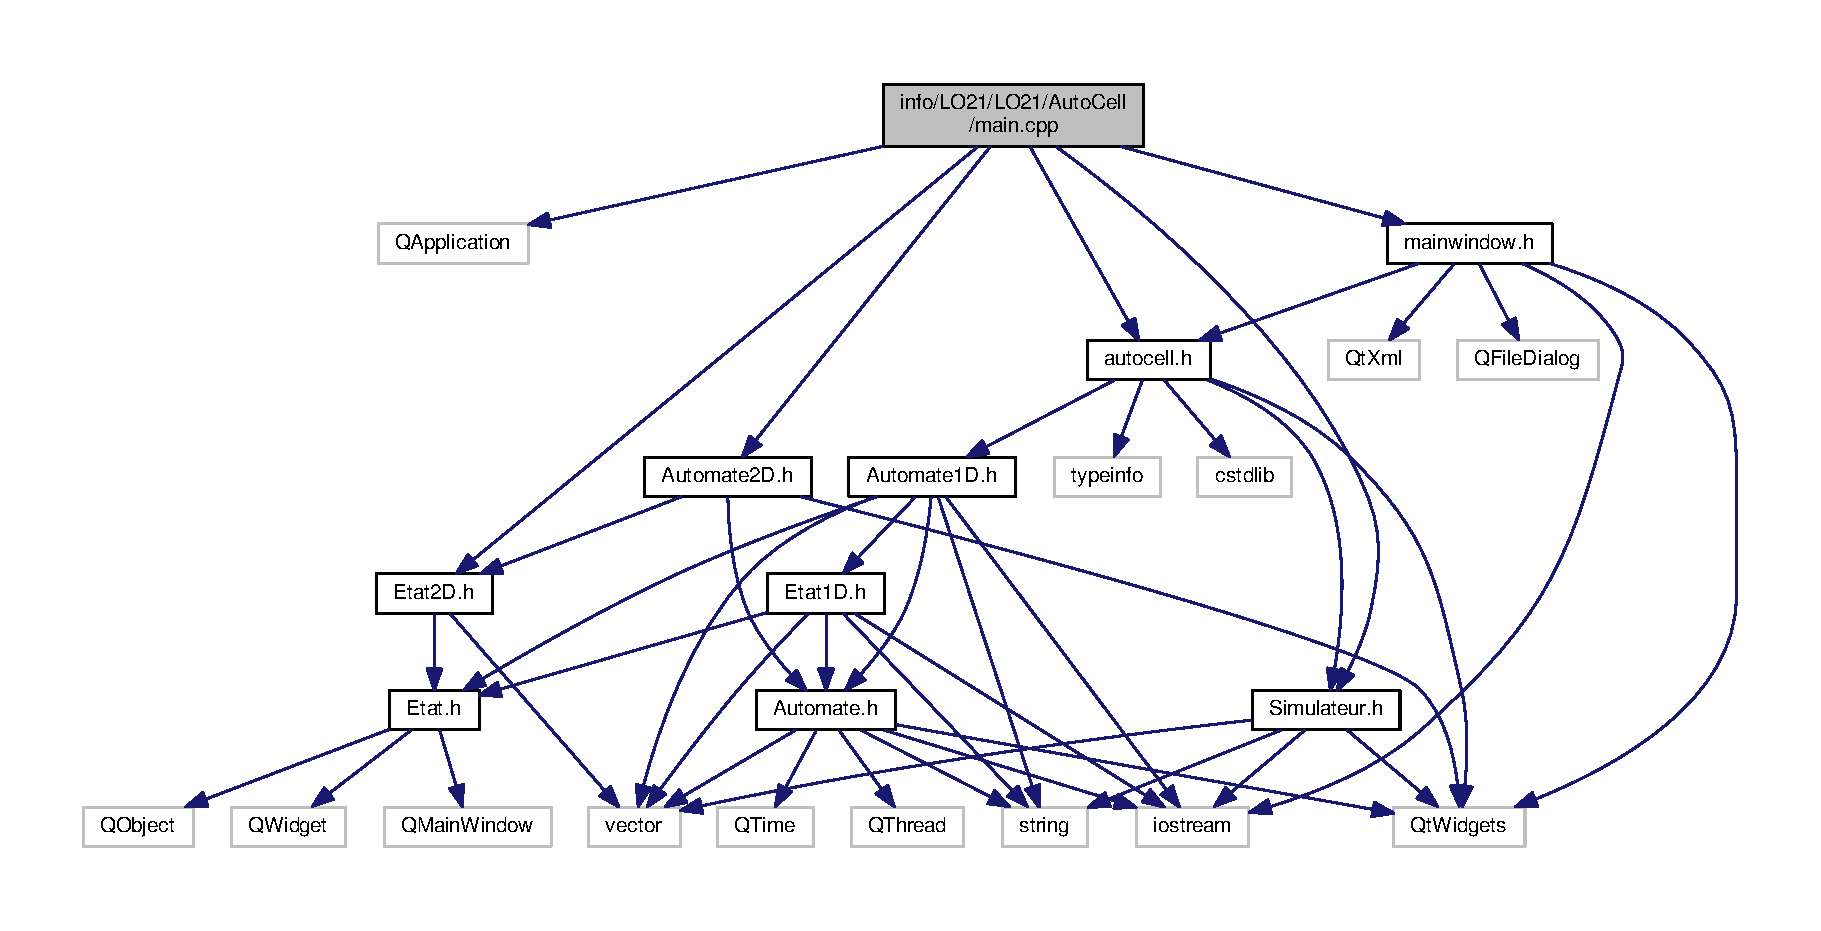
\includegraphics[width=350pt]{main_8cpp__incl}
\end{center}
\end{figure}
\subsection*{Fonctions}
\begin{DoxyCompactItemize}
\item 
int \hyperlink{main_8cpp_a0ddf1224851353fc92bfbff6f499fa97}{main} (int argc, char $\ast$argv\mbox{[}$\,$\mbox{]})
\end{DoxyCompactItemize}


\subsection{Documentation des fonctions}
\index{main.\+cpp@{main.\+cpp}!main@{main}}
\index{main@{main}!main.\+cpp@{main.\+cpp}}
\subsubsection[{\texorpdfstring{main(int argc, char $\ast$argv[])}{main(int argc, char *argv[])}}]{\setlength{\rightskip}{0pt plus 5cm}int main (
\begin{DoxyParamCaption}
\item[{int}]{argc, }
\item[{char $\ast$}]{argv\mbox{[}$\,$\mbox{]}}
\end{DoxyParamCaption}
)}\hypertarget{main_8cpp_a0ddf1224851353fc92bfbff6f499fa97}{}\label{main_8cpp_a0ddf1224851353fc92bfbff6f499fa97}

\hypertarget{mainwindow_8cpp}{}\section{Référence du fichier /home/thomaspaita/\+Bureau/info/\+L\+O21/\+L\+O21/\+Auto\+Cell/mainwindow.cpp}
\label{mainwindow_8cpp}\index{/home/thomaspaita/\+Bureau/info/\+L\+O21/\+L\+O21/\+Auto\+Cell/mainwindow.\+cpp@{/home/thomaspaita/\+Bureau/info/\+L\+O21/\+L\+O21/\+Auto\+Cell/mainwindow.\+cpp}}
{\ttfamily \#include \char`\"{}mainwindow.\+h\char`\"{}}\\*
{\ttfamily \#include \char`\"{}autocell.\+h\char`\"{}}\\*
{\ttfamily \#include $<$iostream$>$}\\*
{\ttfamily \#include $<$typeinfo$>$}\\*
Graphe des dépendances par inclusion de mainwindow.\+cpp\+:
\nopagebreak
\begin{figure}[H]
\begin{center}
\leavevmode
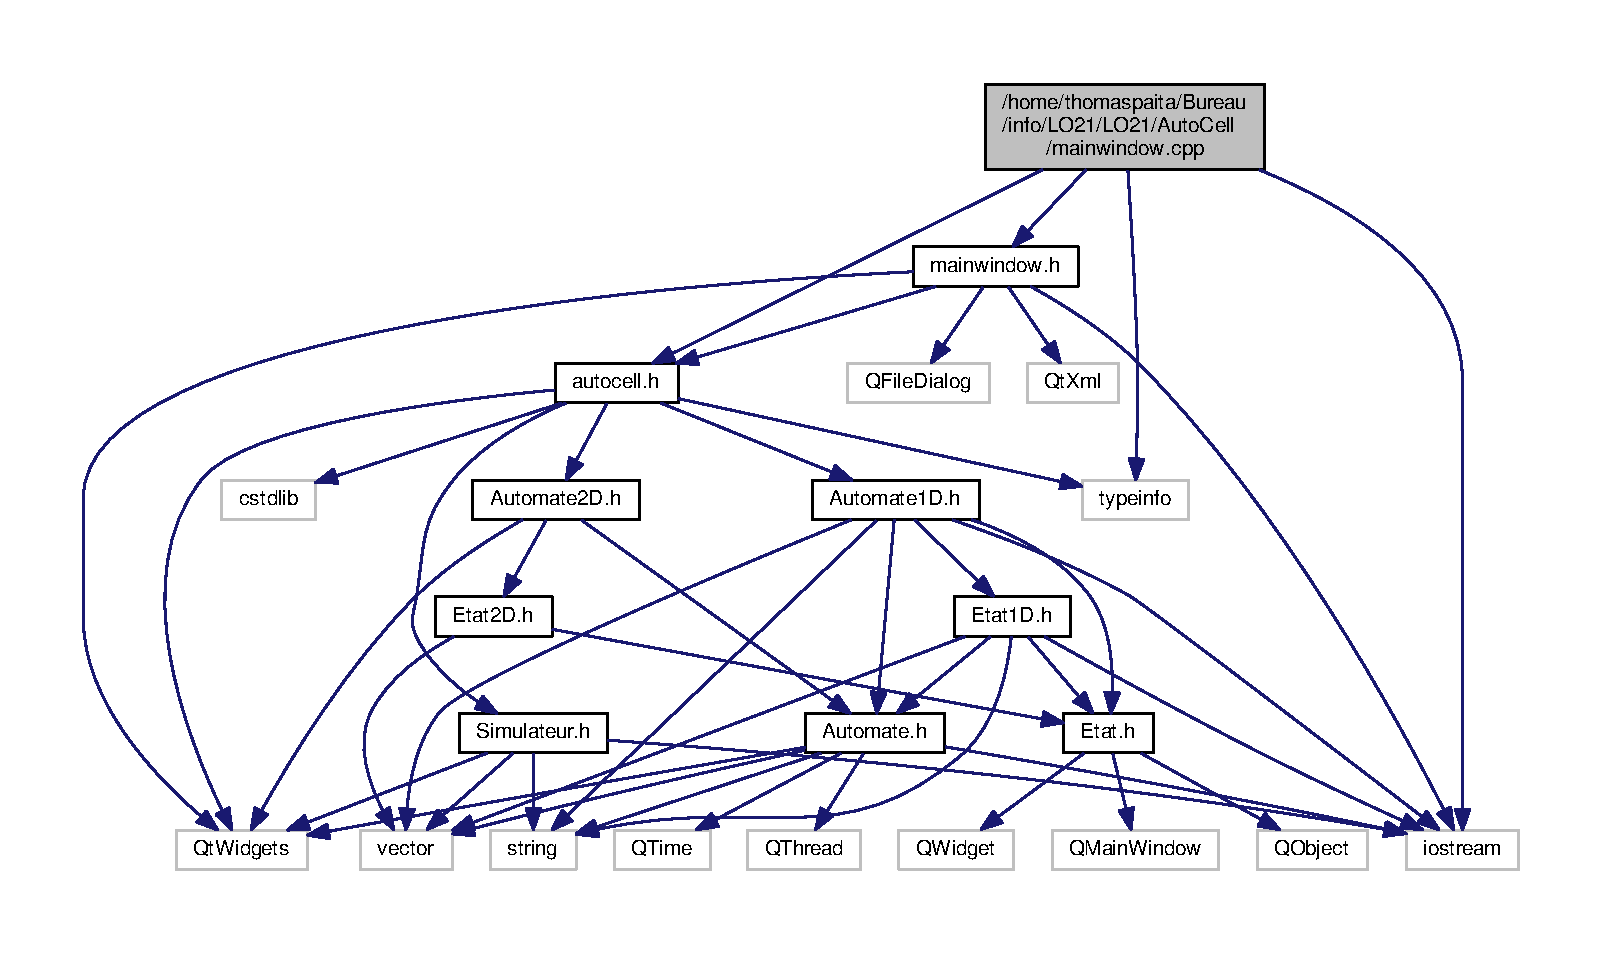
\includegraphics[width=350pt]{mainwindow_8cpp__incl}
\end{center}
\end{figure}

\hypertarget{mainwindow_8h}{}\section{Référence du fichier /home/thomaspaita/\+Bureau/info/\+L\+O21/\+L\+O21/\+Auto\+Cell/mainwindow.h}
\label{mainwindow_8h}\index{/home/thomaspaita/\+Bureau/info/\+L\+O21/\+L\+O21/\+Auto\+Cell/mainwindow.\+h@{/home/thomaspaita/\+Bureau/info/\+L\+O21/\+L\+O21/\+Auto\+Cell/mainwindow.\+h}}
{\ttfamily \#include $<$Qt\+Widgets$>$}\\*
{\ttfamily \#include \char`\"{}autocell.\+h\char`\"{}}\\*
{\ttfamily \#include $<$iostream$>$}\\*
{\ttfamily \#include $<$Qt\+Xml$>$}\\*
{\ttfamily \#include $<$Q\+File\+Dialog$>$}\\*
Graphe des dépendances par inclusion de mainwindow.\+h\+:
\nopagebreak
\begin{figure}[H]
\begin{center}
\leavevmode
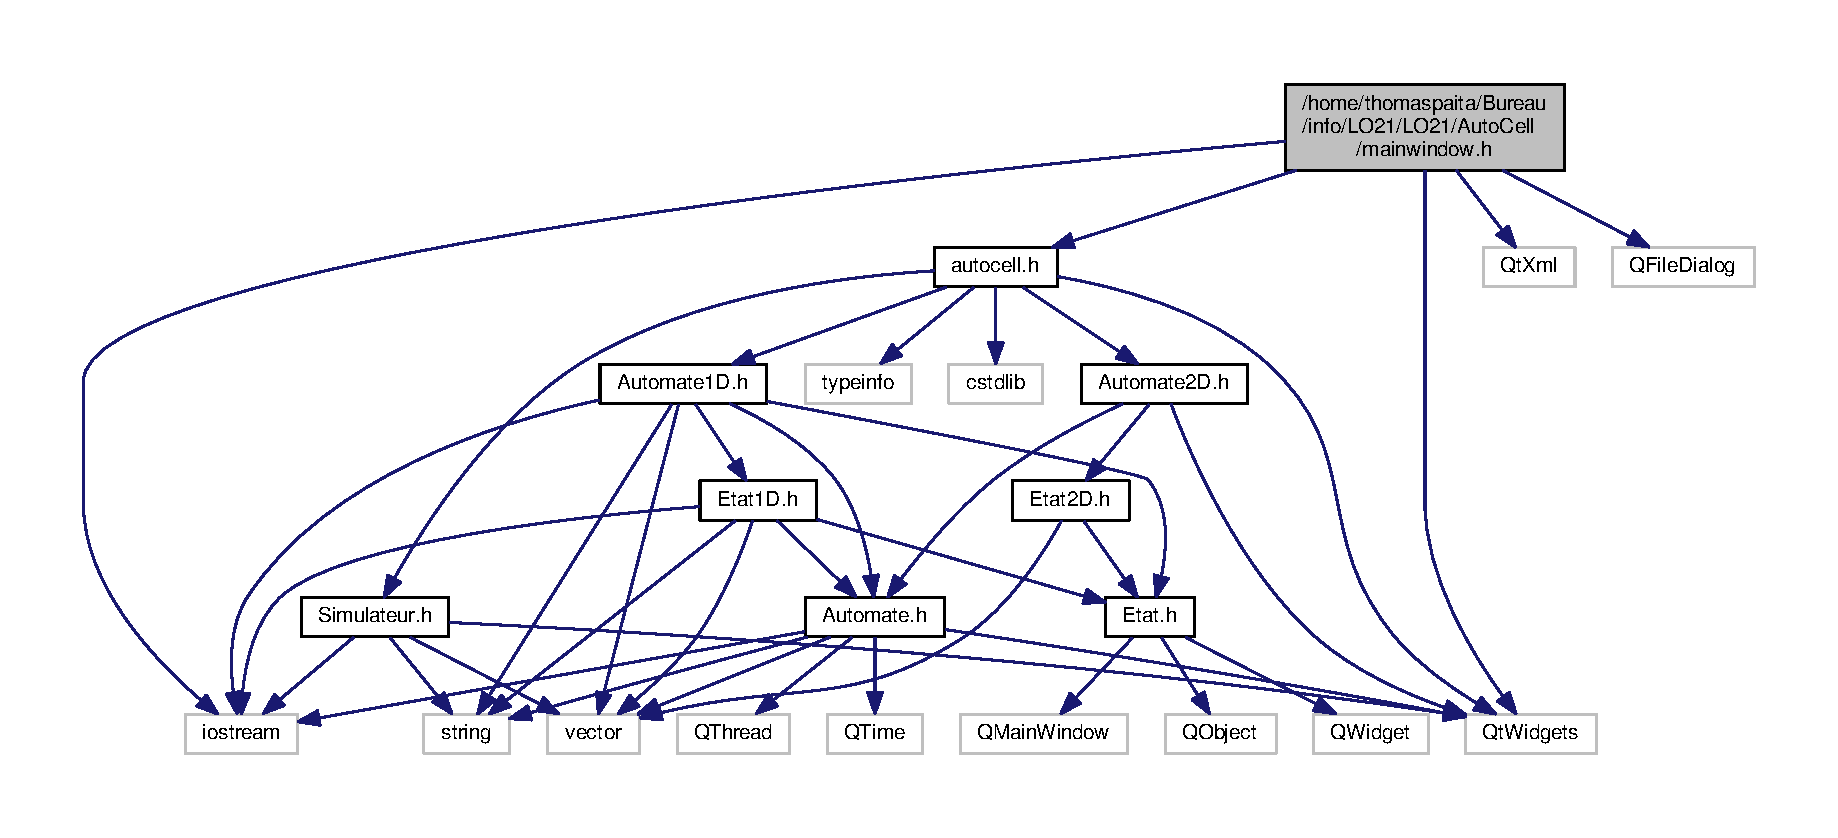
\includegraphics[width=350pt]{mainwindow_8h__incl}
\end{center}
\end{figure}
Ce graphe montre quels fichiers incluent directement ou indirectement ce fichier \+:
\nopagebreak
\begin{figure}[H]
\begin{center}
\leavevmode
\includegraphics[width=350pt]{mainwindow_8h__dep__incl}
\end{center}
\end{figure}
\subsection*{Classes}
\begin{DoxyCompactItemize}
\item 
class \hyperlink{class_main_window}{Main\+Window}
\begin{DoxyCompactList}\small\item\em hérite de Q\+Main\+Window Représente la fenêtre principal de l\textquotesingle{}application \end{DoxyCompactList}\item 
class \hyperlink{class_w_spacer}{W\+Spacer}
\begin{DoxyCompactList}\small\item\em hérite de Q\+Widget met un espace dans la Q\+Tool\+Bar \end{DoxyCompactList}\end{DoxyCompactItemize}

\hypertarget{_simulateur_8cpp}{}\section{Référence du fichier info/\+L\+O21/\+L\+O21/\+Auto\+Cell/\+Simulateur.cpp}
\label{_simulateur_8cpp}\index{info/\+L\+O21/\+L\+O21/\+Auto\+Cell/\+Simulateur.\+cpp@{info/\+L\+O21/\+L\+O21/\+Auto\+Cell/\+Simulateur.\+cpp}}
{\ttfamily \#include \char`\"{}Simulateur.\+h\char`\"{}}\\*
{\ttfamily \#include \char`\"{}Automate1\+D.\+h\char`\"{}}\\*
{\ttfamily \#include \char`\"{}Automate2\+D.\+h\char`\"{}}\\*
{\ttfamily \#include \char`\"{}Etat2\+D.\+h\char`\"{}}\\*
{\ttfamily \#include $<$iostream$>$}\\*
Graphe des dépendances par inclusion de Simulateur.\+cpp\+:\nopagebreak
\begin{figure}[H]
\begin{center}
\leavevmode
\includegraphics[width=350pt]{_simulateur_8cpp__incl}
\end{center}
\end{figure}

\hypertarget{_simulateur_8h}{}\section{Référence du fichier /home/thomaspaita/\+Bureau/info/\+L\+O21/\+L\+O21/\+Auto\+Cell/\+Simulateur.h}
\label{_simulateur_8h}\index{/home/thomaspaita/\+Bureau/info/\+L\+O21/\+L\+O21/\+Auto\+Cell/\+Simulateur.\+h@{/home/thomaspaita/\+Bureau/info/\+L\+O21/\+L\+O21/\+Auto\+Cell/\+Simulateur.\+h}}
{\ttfamily \#include $<$Qt\+Widgets$>$}\\*
{\ttfamily \#include $<$iostream$>$}\\*
{\ttfamily \#include $<$string$>$}\\*
{\ttfamily \#include $<$vector$>$}\\*
Graphe des dépendances par inclusion de Simulateur.\+h\+:
\nopagebreak
\begin{figure}[H]
\begin{center}
\leavevmode
\includegraphics[width=338pt]{_simulateur_8h__incl}
\end{center}
\end{figure}
Ce graphe montre quels fichiers incluent directement ou indirectement ce fichier \+:
\nopagebreak
\begin{figure}[H]
\begin{center}
\leavevmode
\includegraphics[width=350pt]{_simulateur_8h__dep__incl}
\end{center}
\end{figure}
\subsection*{Classes}
\begin{DoxyCompactItemize}
\item 
class \hyperlink{class_automate}{Automate$<$ T $>$}
\begin{DoxyCompactList}\small\item\em Classe Template abstraite. La classe généralise un \hyperlink{class_automate}{Automate} et définie la méthodes virtuelle qui devra être présente et définie dans chaque \hyperlink{class_automate}{Automate}. (run\+Sim()) \end{DoxyCompactList}\item 
class \hyperlink{class_simulateur}{Simulateur$<$ T1, T2 $>$}
\begin{DoxyCompactList}\small\item\em Classe template. Permet de gérer la simulation de n\textquotesingle{}importe quel automate héritant de la Classe \hyperlink{class_automate}{Automate}. \end{DoxyCompactList}\item 
class \hyperlink{class_simulateur}{Simulateur$<$ T1, T2 $>$}
\begin{DoxyCompactList}\small\item\em Classe template. Permet de gérer la simulation de n\textquotesingle{}importe quel automate héritant de la Classe \hyperlink{class_automate}{Automate}. \end{DoxyCompactList}\item 
class \hyperlink{class_simulateur_1_1iterator}{Simulateur$<$ T1, T2 $>$\+::iterator}
\begin{DoxyCompactList}\small\item\em permet le parcourt des états \end{DoxyCompactList}\item 
class \hyperlink{class_simulateur_1_1const__iterator}{Simulateur$<$ T1, T2 $>$\+::const\+\_\+iterator}
\end{DoxyCompactItemize}


\subsection{Description détaillée}
\begin{DoxyVersion}{Version}
1.\+0 
\end{DoxyVersion}

\hypertarget{moc__autocell_8cpp}{}\section{Référence du fichier /home/thomaspaita/\+Bureau/info/\+L\+O21/\+L\+O21/build-\/\+Auto\+Cell-\/\+Desktop-\/\+Debug/moc\+\_\+autocell.cpp}
\label{moc__autocell_8cpp}\index{/home/thomaspaita/\+Bureau/info/\+L\+O21/\+L\+O21/build-\/\+Auto\+Cell-\/\+Desktop-\/\+Debug/moc\+\_\+autocell.\+cpp@{/home/thomaspaita/\+Bureau/info/\+L\+O21/\+L\+O21/build-\/\+Auto\+Cell-\/\+Desktop-\/\+Debug/moc\+\_\+autocell.\+cpp}}
{\ttfamily \#include \char`\"{}../\+Auto\+Cell/autocell.\+h\char`\"{}}\\*
{\ttfamily \#include $<$Qt\+Core/qbytearray.\+h$>$}\\*
{\ttfamily \#include $<$Qt\+Core/qmetatype.\+h$>$}\\*
Graphe des dépendances par inclusion de moc\+\_\+autocell.\+cpp\+:
\nopagebreak
\begin{figure}[H]
\begin{center}
\leavevmode
\includegraphics[width=350pt]{moc__autocell_8cpp__incl}
\end{center}
\end{figure}
\subsection*{Classes}
\begin{DoxyCompactItemize}
\item 
struct \hyperlink{structqt__meta__stringdata___autocell__t}{qt\+\_\+meta\+\_\+stringdata\+\_\+\+Autocell\+\_\+t}
\item 
struct \hyperlink{structqt__meta__stringdata___autocell1_d__t}{qt\+\_\+meta\+\_\+stringdata\+\_\+\+Autocell1\+D\+\_\+t}
\item 
struct \hyperlink{structqt__meta__stringdata___autocell2_d__t}{qt\+\_\+meta\+\_\+stringdata\+\_\+\+Autocell2\+D\+\_\+t}
\item 
struct \hyperlink{structqt__meta__stringdata___regle2_d__t}{qt\+\_\+meta\+\_\+stringdata\+\_\+\+Regle2\+D\+\_\+t}
\end{DoxyCompactItemize}
\subsection*{Macros}
\begin{DoxyCompactItemize}
\item 
\#define \hyperlink{moc__autocell_8cpp_a75bb9482d242cde0a06c9dbdc6b83abe}{Q\+T\+\_\+\+M\+O\+C\+\_\+\+L\+I\+T\+E\+R\+AL}(idx,  ofs,  len)
\item 
\#define \hyperlink{moc__autocell_8cpp_a75bb9482d242cde0a06c9dbdc6b83abe}{Q\+T\+\_\+\+M\+O\+C\+\_\+\+L\+I\+T\+E\+R\+AL}(idx,  ofs,  len)
\item 
\#define \hyperlink{moc__autocell_8cpp_a75bb9482d242cde0a06c9dbdc6b83abe}{Q\+T\+\_\+\+M\+O\+C\+\_\+\+L\+I\+T\+E\+R\+AL}(idx,  ofs,  len)
\item 
\#define \hyperlink{moc__autocell_8cpp_a75bb9482d242cde0a06c9dbdc6b83abe}{Q\+T\+\_\+\+M\+O\+C\+\_\+\+L\+I\+T\+E\+R\+AL}(idx,  ofs,  len)
\end{DoxyCompactItemize}
\subsection*{Variables}
\begin{DoxyCompactItemize}
\item 
static const \hyperlink{structqt__meta__stringdata___autocell__t}{qt\+\_\+meta\+\_\+stringdata\+\_\+\+Autocell\+\_\+t} \hyperlink{moc__autocell_8cpp_a63d164cf84bfa7fef91fc48821d2f838}{qt\+\_\+meta\+\_\+stringdata\+\_\+\+Autocell}
\item 
static const uint \hyperlink{moc__autocell_8cpp_abd0ec0a7eff5e29520a7ea6ce3956d44}{qt\+\_\+meta\+\_\+data\+\_\+\+Autocell} \mbox{[}$\,$\mbox{]}
\item 
static const \hyperlink{structqt__meta__stringdata___autocell1_d__t}{qt\+\_\+meta\+\_\+stringdata\+\_\+\+Autocell1\+D\+\_\+t} \hyperlink{moc__autocell_8cpp_acabbaf4e8113f2ba2d471ebbfce096e8}{qt\+\_\+meta\+\_\+stringdata\+\_\+\+Autocell1D}
\item 
static const uint \hyperlink{moc__autocell_8cpp_a482c94390597ceab1de31147c54e8d97}{qt\+\_\+meta\+\_\+data\+\_\+\+Autocell1D} \mbox{[}$\,$\mbox{]}
\item 
static const \hyperlink{structqt__meta__stringdata___autocell2_d__t}{qt\+\_\+meta\+\_\+stringdata\+\_\+\+Autocell2\+D\+\_\+t} \hyperlink{moc__autocell_8cpp_a4cf37aa8fc6405e0bcdf1956c0337733}{qt\+\_\+meta\+\_\+stringdata\+\_\+\+Autocell2D}
\item 
static const uint \hyperlink{moc__autocell_8cpp_aa4cdc5583ddd927e4db9312c7d82ce09}{qt\+\_\+meta\+\_\+data\+\_\+\+Autocell2D} \mbox{[}$\,$\mbox{]}
\item 
static const \hyperlink{structqt__meta__stringdata___regle2_d__t}{qt\+\_\+meta\+\_\+stringdata\+\_\+\+Regle2\+D\+\_\+t} \hyperlink{moc__autocell_8cpp_ae4a3c712fad46dbcfbb97f1729b31ba4}{qt\+\_\+meta\+\_\+stringdata\+\_\+\+Regle2D}
\item 
static const uint \hyperlink{moc__autocell_8cpp_a6ad67278e9b02dc321fb63777c97a7a4}{qt\+\_\+meta\+\_\+data\+\_\+\+Regle2D} \mbox{[}$\,$\mbox{]}
\end{DoxyCompactItemize}


\subsection{Documentation des macros}
\index{moc\+\_\+autocell.\+cpp@{moc\+\_\+autocell.\+cpp}!Q\+T\+\_\+\+M\+O\+C\+\_\+\+L\+I\+T\+E\+R\+AL@{Q\+T\+\_\+\+M\+O\+C\+\_\+\+L\+I\+T\+E\+R\+AL}}
\index{Q\+T\+\_\+\+M\+O\+C\+\_\+\+L\+I\+T\+E\+R\+AL@{Q\+T\+\_\+\+M\+O\+C\+\_\+\+L\+I\+T\+E\+R\+AL}!moc\+\_\+autocell.\+cpp@{moc\+\_\+autocell.\+cpp}}
\subsubsection[{\texorpdfstring{Q\+T\+\_\+\+M\+O\+C\+\_\+\+L\+I\+T\+E\+R\+AL}{QT_MOC_LITERAL}}]{\setlength{\rightskip}{0pt plus 5cm}\#define Q\+T\+\_\+\+M\+O\+C\+\_\+\+L\+I\+T\+E\+R\+AL(
\begin{DoxyParamCaption}
\item[{}]{idx, }
\item[{}]{ofs, }
\item[{}]{len}
\end{DoxyParamCaption}
)}\hypertarget{moc__autocell_8cpp_a75bb9482d242cde0a06c9dbdc6b83abe}{}\label{moc__autocell_8cpp_a75bb9482d242cde0a06c9dbdc6b83abe}
{\bfseries Valeur \+:}
\begin{DoxyCode}
Q\_STATIC\_BYTE\_ARRAY\_DATA\_HEADER\_INITIALIZER\_WITH\_OFFSET(len, \(\backslash\)
    qptrdiff(offsetof(\hyperlink{structqt__meta__stringdata___autocell__t}{qt\_meta\_stringdata\_Autocell\_t}, stringdata0) + ofs \(\backslash\)
        - idx * \textcolor{keyword}{sizeof}(QByteArrayData)) \(\backslash\)
    )
\end{DoxyCode}
\index{moc\+\_\+autocell.\+cpp@{moc\+\_\+autocell.\+cpp}!Q\+T\+\_\+\+M\+O\+C\+\_\+\+L\+I\+T\+E\+R\+AL@{Q\+T\+\_\+\+M\+O\+C\+\_\+\+L\+I\+T\+E\+R\+AL}}
\index{Q\+T\+\_\+\+M\+O\+C\+\_\+\+L\+I\+T\+E\+R\+AL@{Q\+T\+\_\+\+M\+O\+C\+\_\+\+L\+I\+T\+E\+R\+AL}!moc\+\_\+autocell.\+cpp@{moc\+\_\+autocell.\+cpp}}
\subsubsection[{\texorpdfstring{Q\+T\+\_\+\+M\+O\+C\+\_\+\+L\+I\+T\+E\+R\+AL}{QT_MOC_LITERAL}}]{\setlength{\rightskip}{0pt plus 5cm}\#define Q\+T\+\_\+\+M\+O\+C\+\_\+\+L\+I\+T\+E\+R\+AL(
\begin{DoxyParamCaption}
\item[{}]{idx, }
\item[{}]{ofs, }
\item[{}]{len}
\end{DoxyParamCaption}
)}\hypertarget{moc__autocell_8cpp_a75bb9482d242cde0a06c9dbdc6b83abe}{}\label{moc__autocell_8cpp_a75bb9482d242cde0a06c9dbdc6b83abe}
{\bfseries Valeur \+:}
\begin{DoxyCode}
Q\_STATIC\_BYTE\_ARRAY\_DATA\_HEADER\_INITIALIZER\_WITH\_OFFSET(len, \(\backslash\)
    qptrdiff(offsetof(\hyperlink{structqt__meta__stringdata___autocell1_d__t}{qt\_meta\_stringdata\_Autocell1D\_t}, stringdata0) + ofs \(\backslash\)
        - idx * \textcolor{keyword}{sizeof}(QByteArrayData)) \(\backslash\)
    )
\end{DoxyCode}
\index{moc\+\_\+autocell.\+cpp@{moc\+\_\+autocell.\+cpp}!Q\+T\+\_\+\+M\+O\+C\+\_\+\+L\+I\+T\+E\+R\+AL@{Q\+T\+\_\+\+M\+O\+C\+\_\+\+L\+I\+T\+E\+R\+AL}}
\index{Q\+T\+\_\+\+M\+O\+C\+\_\+\+L\+I\+T\+E\+R\+AL@{Q\+T\+\_\+\+M\+O\+C\+\_\+\+L\+I\+T\+E\+R\+AL}!moc\+\_\+autocell.\+cpp@{moc\+\_\+autocell.\+cpp}}
\subsubsection[{\texorpdfstring{Q\+T\+\_\+\+M\+O\+C\+\_\+\+L\+I\+T\+E\+R\+AL}{QT_MOC_LITERAL}}]{\setlength{\rightskip}{0pt plus 5cm}\#define Q\+T\+\_\+\+M\+O\+C\+\_\+\+L\+I\+T\+E\+R\+AL(
\begin{DoxyParamCaption}
\item[{}]{idx, }
\item[{}]{ofs, }
\item[{}]{len}
\end{DoxyParamCaption}
)}\hypertarget{moc__autocell_8cpp_a75bb9482d242cde0a06c9dbdc6b83abe}{}\label{moc__autocell_8cpp_a75bb9482d242cde0a06c9dbdc6b83abe}
{\bfseries Valeur \+:}
\begin{DoxyCode}
Q\_STATIC\_BYTE\_ARRAY\_DATA\_HEADER\_INITIALIZER\_WITH\_OFFSET(len, \(\backslash\)
    qptrdiff(offsetof(\hyperlink{structqt__meta__stringdata___autocell2_d__t}{qt\_meta\_stringdata\_Autocell2D\_t}, stringdata0) + ofs \(\backslash\)
        - idx * \textcolor{keyword}{sizeof}(QByteArrayData)) \(\backslash\)
    )
\end{DoxyCode}
\index{moc\+\_\+autocell.\+cpp@{moc\+\_\+autocell.\+cpp}!Q\+T\+\_\+\+M\+O\+C\+\_\+\+L\+I\+T\+E\+R\+AL@{Q\+T\+\_\+\+M\+O\+C\+\_\+\+L\+I\+T\+E\+R\+AL}}
\index{Q\+T\+\_\+\+M\+O\+C\+\_\+\+L\+I\+T\+E\+R\+AL@{Q\+T\+\_\+\+M\+O\+C\+\_\+\+L\+I\+T\+E\+R\+AL}!moc\+\_\+autocell.\+cpp@{moc\+\_\+autocell.\+cpp}}
\subsubsection[{\texorpdfstring{Q\+T\+\_\+\+M\+O\+C\+\_\+\+L\+I\+T\+E\+R\+AL}{QT_MOC_LITERAL}}]{\setlength{\rightskip}{0pt plus 5cm}\#define Q\+T\+\_\+\+M\+O\+C\+\_\+\+L\+I\+T\+E\+R\+AL(
\begin{DoxyParamCaption}
\item[{}]{idx, }
\item[{}]{ofs, }
\item[{}]{len}
\end{DoxyParamCaption}
)}\hypertarget{moc__autocell_8cpp_a75bb9482d242cde0a06c9dbdc6b83abe}{}\label{moc__autocell_8cpp_a75bb9482d242cde0a06c9dbdc6b83abe}
{\bfseries Valeur \+:}
\begin{DoxyCode}
Q\_STATIC\_BYTE\_ARRAY\_DATA\_HEADER\_INITIALIZER\_WITH\_OFFSET(len, \(\backslash\)
    qptrdiff(offsetof(\hyperlink{structqt__meta__stringdata___regle2_d__t}{qt\_meta\_stringdata\_Regle2D\_t}, stringdata0) + ofs \(\backslash\)
        - idx * \textcolor{keyword}{sizeof}(QByteArrayData)) \(\backslash\)
    )
\end{DoxyCode}


\subsection{Documentation des variables}
\index{moc\+\_\+autocell.\+cpp@{moc\+\_\+autocell.\+cpp}!qt\+\_\+meta\+\_\+data\+\_\+\+Autocell@{qt\+\_\+meta\+\_\+data\+\_\+\+Autocell}}
\index{qt\+\_\+meta\+\_\+data\+\_\+\+Autocell@{qt\+\_\+meta\+\_\+data\+\_\+\+Autocell}!moc\+\_\+autocell.\+cpp@{moc\+\_\+autocell.\+cpp}}
\subsubsection[{\texorpdfstring{qt\+\_\+meta\+\_\+data\+\_\+\+Autocell}{qt_meta_data_Autocell}}]{\setlength{\rightskip}{0pt plus 5cm}const uint qt\+\_\+meta\+\_\+data\+\_\+\+Autocell\mbox{[}$\,$\mbox{]}\hspace{0.3cm}{\ttfamily [static]}}\hypertarget{moc__autocell_8cpp_abd0ec0a7eff5e29520a7ea6ce3956d44}{}\label{moc__autocell_8cpp_abd0ec0a7eff5e29520a7ea6ce3956d44}
{\bfseries Valeur initiale \+:}
\begin{DoxyCode}
= \{

 
       7,       
       0,       
       0,    0, 
       2,   14, 
       0,    0, 
       0,    0, 
       0,    0, 
       0,       
       1,       

 
       1,    0,   24,    2, 0x06 ,

 
       3,    2,   25,    2, 0x0a ,

 
    QMetaType::Void,

 
    QMetaType::Void, QMetaType::Int, QMetaType::Int,    4,    5,

       0        
\}
\end{DoxyCode}
\index{moc\+\_\+autocell.\+cpp@{moc\+\_\+autocell.\+cpp}!qt\+\_\+meta\+\_\+data\+\_\+\+Autocell1D@{qt\+\_\+meta\+\_\+data\+\_\+\+Autocell1D}}
\index{qt\+\_\+meta\+\_\+data\+\_\+\+Autocell1D@{qt\+\_\+meta\+\_\+data\+\_\+\+Autocell1D}!moc\+\_\+autocell.\+cpp@{moc\+\_\+autocell.\+cpp}}
\subsubsection[{\texorpdfstring{qt\+\_\+meta\+\_\+data\+\_\+\+Autocell1D}{qt_meta_data_Autocell1D}}]{\setlength{\rightskip}{0pt plus 5cm}const uint qt\+\_\+meta\+\_\+data\+\_\+\+Autocell1D\mbox{[}$\,$\mbox{]}\hspace{0.3cm}{\ttfamily [static]}}\hypertarget{moc__autocell_8cpp_a482c94390597ceab1de31147c54e8d97}{}\label{moc__autocell_8cpp_a482c94390597ceab1de31147c54e8d97}
{\bfseries Valeur initiale \+:}
\begin{DoxyCode}
= \{

 
       7,       
       0,       
       0,    0, 
       1,   14, 
       0,    0, 
       0,    0, 
       0,    0, 
       0,       
       0,       

 
       1,    2,   19,    2, 0x0a ,

 
    QMetaType::Void, QMetaType::Int, QMetaType::Int,    3,    4,

       0        
\}
\end{DoxyCode}
\index{moc\+\_\+autocell.\+cpp@{moc\+\_\+autocell.\+cpp}!qt\+\_\+meta\+\_\+data\+\_\+\+Autocell2D@{qt\+\_\+meta\+\_\+data\+\_\+\+Autocell2D}}
\index{qt\+\_\+meta\+\_\+data\+\_\+\+Autocell2D@{qt\+\_\+meta\+\_\+data\+\_\+\+Autocell2D}!moc\+\_\+autocell.\+cpp@{moc\+\_\+autocell.\+cpp}}
\subsubsection[{\texorpdfstring{qt\+\_\+meta\+\_\+data\+\_\+\+Autocell2D}{qt_meta_data_Autocell2D}}]{\setlength{\rightskip}{0pt plus 5cm}const uint qt\+\_\+meta\+\_\+data\+\_\+\+Autocell2D\mbox{[}$\,$\mbox{]}\hspace{0.3cm}{\ttfamily [static]}}\hypertarget{moc__autocell_8cpp_aa4cdc5583ddd927e4db9312c7d82ce09}{}\label{moc__autocell_8cpp_aa4cdc5583ddd927e4db9312c7d82ce09}
{\bfseries Valeur initiale \+:}
\begin{DoxyCode}
= \{

 
       7,       
       0,       
       0,    0, 
       4,   14, 
       0,    0, 
       0,    0, 
       0,    0, 
       0,       
       0,       

 
       1,    2,   34,    2, 0x0a ,
       5,    0,   39,    2, 0x0a ,
       6,    0,   40,    2, 0x0a ,
       7,    2,   41,    2, 0x0a ,

 
    QMetaType::Void, QMetaType::Int, QMetaType::Int,    3,    4,
    QMetaType::Void,
    QMetaType::Void,
    QMetaType::Void, 0x80000000 | 8, 0x80000000 | 10,    9,   11,

       0        
\}
\end{DoxyCode}
\index{moc\+\_\+autocell.\+cpp@{moc\+\_\+autocell.\+cpp}!qt\+\_\+meta\+\_\+data\+\_\+\+Regle2D@{qt\+\_\+meta\+\_\+data\+\_\+\+Regle2D}}
\index{qt\+\_\+meta\+\_\+data\+\_\+\+Regle2D@{qt\+\_\+meta\+\_\+data\+\_\+\+Regle2D}!moc\+\_\+autocell.\+cpp@{moc\+\_\+autocell.\+cpp}}
\subsubsection[{\texorpdfstring{qt\+\_\+meta\+\_\+data\+\_\+\+Regle2D}{qt_meta_data_Regle2D}}]{\setlength{\rightskip}{0pt plus 5cm}const uint qt\+\_\+meta\+\_\+data\+\_\+\+Regle2D\mbox{[}$\,$\mbox{]}\hspace{0.3cm}{\ttfamily [static]}}\hypertarget{moc__autocell_8cpp_a6ad67278e9b02dc321fb63777c97a7a4}{}\label{moc__autocell_8cpp_a6ad67278e9b02dc321fb63777c97a7a4}
\index{moc\+\_\+autocell.\+cpp@{moc\+\_\+autocell.\+cpp}!qt\+\_\+meta\+\_\+stringdata\+\_\+\+Autocell@{qt\+\_\+meta\+\_\+stringdata\+\_\+\+Autocell}}
\index{qt\+\_\+meta\+\_\+stringdata\+\_\+\+Autocell@{qt\+\_\+meta\+\_\+stringdata\+\_\+\+Autocell}!moc\+\_\+autocell.\+cpp@{moc\+\_\+autocell.\+cpp}}
\subsubsection[{\texorpdfstring{qt\+\_\+meta\+\_\+stringdata\+\_\+\+Autocell}{qt_meta_stringdata_Autocell}}]{\setlength{\rightskip}{0pt plus 5cm}const {\bf qt\+\_\+meta\+\_\+stringdata\+\_\+\+Autocell\+\_\+t} qt\+\_\+meta\+\_\+stringdata\+\_\+\+Autocell\hspace{0.3cm}{\ttfamily [static]}}\hypertarget{moc__autocell_8cpp_a63d164cf84bfa7fef91fc48821d2f838}{}\label{moc__autocell_8cpp_a63d164cf84bfa7fef91fc48821d2f838}
{\bfseries Valeur initiale \+:}
\begin{DoxyCode}
= \{
    \{
\hyperlink{moc__autocell_8cpp_a75bb9482d242cde0a06c9dbdc6b83abe}{QT\_MOC\_LITERAL}(0, 0, 8), 
\hyperlink{moc__autocell_8cpp_a75bb9482d242cde0a06c9dbdc6b83abe}{QT\_MOC\_LITERAL}(1, 9, 6), 
\hyperlink{moc__autocell_8cpp_a75bb9482d242cde0a06c9dbdc6b83abe}{QT\_MOC\_LITERAL}(2, 16, 0), 
\hyperlink{moc__autocell_8cpp_a75bb9482d242cde0a06c9dbdc6b83abe}{QT\_MOC\_LITERAL}(3, 17, 12), 
\hyperlink{moc__autocell_8cpp_a75bb9482d242cde0a06c9dbdc6b83abe}{QT\_MOC\_LITERAL}(4, 30, 1), 
\hyperlink{moc__autocell_8cpp_a75bb9482d242cde0a06c9dbdc6b83abe}{QT\_MOC\_LITERAL}(5, 32, 1) 

    \},
    \textcolor{stringliteral}{"Autocell\(\backslash\)0endSim\(\backslash\)0\(\backslash\)0cellSelected\(\backslash\)0a\(\backslash\)0b"}
\}
\end{DoxyCode}
\index{moc\+\_\+autocell.\+cpp@{moc\+\_\+autocell.\+cpp}!qt\+\_\+meta\+\_\+stringdata\+\_\+\+Autocell1D@{qt\+\_\+meta\+\_\+stringdata\+\_\+\+Autocell1D}}
\index{qt\+\_\+meta\+\_\+stringdata\+\_\+\+Autocell1D@{qt\+\_\+meta\+\_\+stringdata\+\_\+\+Autocell1D}!moc\+\_\+autocell.\+cpp@{moc\+\_\+autocell.\+cpp}}
\subsubsection[{\texorpdfstring{qt\+\_\+meta\+\_\+stringdata\+\_\+\+Autocell1D}{qt_meta_stringdata_Autocell1D}}]{\setlength{\rightskip}{0pt plus 5cm}const {\bf qt\+\_\+meta\+\_\+stringdata\+\_\+\+Autocell1\+D\+\_\+t} qt\+\_\+meta\+\_\+stringdata\+\_\+\+Autocell1D\hspace{0.3cm}{\ttfamily [static]}}\hypertarget{moc__autocell_8cpp_acabbaf4e8113f2ba2d471ebbfce096e8}{}\label{moc__autocell_8cpp_acabbaf4e8113f2ba2d471ebbfce096e8}
{\bfseries Valeur initiale \+:}
\begin{DoxyCode}
= \{
    \{
\hyperlink{moc__autocell_8cpp_a75bb9482d242cde0a06c9dbdc6b83abe}{QT\_MOC\_LITERAL}(0, 0, 10), 
\hyperlink{moc__autocell_8cpp_a75bb9482d242cde0a06c9dbdc6b83abe}{QT\_MOC\_LITERAL}(1, 11, 12), 
\hyperlink{moc__autocell_8cpp_a75bb9482d242cde0a06c9dbdc6b83abe}{QT\_MOC\_LITERAL}(2, 24, 0), 
\hyperlink{moc__autocell_8cpp_a75bb9482d242cde0a06c9dbdc6b83abe}{QT\_MOC\_LITERAL}(3, 25, 1), 
\hyperlink{moc__autocell_8cpp_a75bb9482d242cde0a06c9dbdc6b83abe}{QT\_MOC\_LITERAL}(4, 27, 1) 

    \},
    \textcolor{stringliteral}{"Autocell1D\(\backslash\)0cellSelected\(\backslash\)0\(\backslash\)0a\(\backslash\)0b"}
\}
\end{DoxyCode}
\index{moc\+\_\+autocell.\+cpp@{moc\+\_\+autocell.\+cpp}!qt\+\_\+meta\+\_\+stringdata\+\_\+\+Autocell2D@{qt\+\_\+meta\+\_\+stringdata\+\_\+\+Autocell2D}}
\index{qt\+\_\+meta\+\_\+stringdata\+\_\+\+Autocell2D@{qt\+\_\+meta\+\_\+stringdata\+\_\+\+Autocell2D}!moc\+\_\+autocell.\+cpp@{moc\+\_\+autocell.\+cpp}}
\subsubsection[{\texorpdfstring{qt\+\_\+meta\+\_\+stringdata\+\_\+\+Autocell2D}{qt_meta_stringdata_Autocell2D}}]{\setlength{\rightskip}{0pt plus 5cm}const {\bf qt\+\_\+meta\+\_\+stringdata\+\_\+\+Autocell2\+D\+\_\+t} qt\+\_\+meta\+\_\+stringdata\+\_\+\+Autocell2D\hspace{0.3cm}{\ttfamily [static]}}\hypertarget{moc__autocell_8cpp_a4cf37aa8fc6405e0bcdf1956c0337733}{}\label{moc__autocell_8cpp_a4cf37aa8fc6405e0bcdf1956c0337733}
{\bfseries Valeur initiale \+:}
\begin{DoxyCode}
= \{
    \{
\hyperlink{moc__autocell_8cpp_a75bb9482d242cde0a06c9dbdc6b83abe}{QT\_MOC\_LITERAL}(0, 0, 10), 
\hyperlink{moc__autocell_8cpp_a75bb9482d242cde0a06c9dbdc6b83abe}{QT\_MOC\_LITERAL}(1, 11, 12), 
\hyperlink{moc__autocell_8cpp_a75bb9482d242cde0a06c9dbdc6b83abe}{QT\_MOC\_LITERAL}(2, 24, 0), 
\hyperlink{moc__autocell_8cpp_a75bb9482d242cde0a06c9dbdc6b83abe}{QT\_MOC\_LITERAL}(3, 25, 1), 
\hyperlink{moc__autocell_8cpp_a75bb9482d242cde0a06c9dbdc6b83abe}{QT\_MOC\_LITERAL}(4, 27, 1), 
\hyperlink{moc__autocell_8cpp_a75bb9482d242cde0a06c9dbdc6b83abe}{QT\_MOC\_LITERAL}(5, 29, 5), 
\hyperlink{moc__autocell_8cpp_a75bb9482d242cde0a06c9dbdc6b83abe}{QT\_MOC\_LITERAL}(6, 35, 6), 
\hyperlink{moc__autocell_8cpp_a75bb9482d242cde0a06c9dbdc6b83abe}{QT\_MOC\_LITERAL}(7, 42, 11), 
\hyperlink{moc__autocell_8cpp_a75bb9482d242cde0a06c9dbdc6b83abe}{QT\_MOC\_LITERAL}(8, 54, 45), 
\hyperlink{moc__autocell_8cpp_a75bb9482d242cde0a06c9dbdc6b83abe}{QT\_MOC\_LITERAL}(9, 100, 1), 
\hyperlink{moc__autocell_8cpp_a75bb9482d242cde0a06c9dbdc6b83abe}{QT\_MOC\_LITERAL}(10, 102, 24), 
\hyperlink{moc__autocell_8cpp_a75bb9482d242cde0a06c9dbdc6b83abe}{QT\_MOC\_LITERAL}(11, 127, 1) 

    \},
    \textcolor{stringliteral}{"Autocell2D\(\backslash\)0cellSelected\(\backslash\)0\(\backslash\)0a\(\backslash\)0b\(\backslash\)0clear\(\backslash\)0"}
    \textcolor{stringliteral}{"runSim\(\backslash\)0changeRegle\(\backslash\)0"}
    \textcolor{stringliteral}{"std::vector<std::vector<unsigned short int> >\(\backslash\)0"}
    \textcolor{stringliteral}{"r\(\backslash\)0std::vector<std::string>\(\backslash\)0c"}
\}
\end{DoxyCode}
\index{moc\+\_\+autocell.\+cpp@{moc\+\_\+autocell.\+cpp}!qt\+\_\+meta\+\_\+stringdata\+\_\+\+Regle2D@{qt\+\_\+meta\+\_\+stringdata\+\_\+\+Regle2D}}
\index{qt\+\_\+meta\+\_\+stringdata\+\_\+\+Regle2D@{qt\+\_\+meta\+\_\+stringdata\+\_\+\+Regle2D}!moc\+\_\+autocell.\+cpp@{moc\+\_\+autocell.\+cpp}}
\subsubsection[{\texorpdfstring{qt\+\_\+meta\+\_\+stringdata\+\_\+\+Regle2D}{qt_meta_stringdata_Regle2D}}]{\setlength{\rightskip}{0pt plus 5cm}const {\bf qt\+\_\+meta\+\_\+stringdata\+\_\+\+Regle2\+D\+\_\+t} qt\+\_\+meta\+\_\+stringdata\+\_\+\+Regle2D\hspace{0.3cm}{\ttfamily [static]}}\hypertarget{moc__autocell_8cpp_ae4a3c712fad46dbcfbb97f1729b31ba4}{}\label{moc__autocell_8cpp_ae4a3c712fad46dbcfbb97f1729b31ba4}
{\bfseries Valeur initiale \+:}
\begin{DoxyCode}
= \{
    \{
\hyperlink{moc__autocell_8cpp_a75bb9482d242cde0a06c9dbdc6b83abe}{QT\_MOC\_LITERAL}(0, 0, 7), 
\hyperlink{moc__autocell_8cpp_a75bb9482d242cde0a06c9dbdc6b83abe}{QT\_MOC\_LITERAL}(1, 8, 10), 
\hyperlink{moc__autocell_8cpp_a75bb9482d242cde0a06c9dbdc6b83abe}{QT\_MOC\_LITERAL}(2, 19, 0), 
\hyperlink{moc__autocell_8cpp_a75bb9482d242cde0a06c9dbdc6b83abe}{QT\_MOC\_LITERAL}(3, 20, 45), 
\hyperlink{moc__autocell_8cpp_a75bb9482d242cde0a06c9dbdc6b83abe}{QT\_MOC\_LITERAL}(4, 66, 24), 
\hyperlink{moc__autocell_8cpp_a75bb9482d242cde0a06c9dbdc6b83abe}{QT\_MOC\_LITERAL}(5, 91, 6), 
\hyperlink{moc__autocell_8cpp_a75bb9482d242cde0a06c9dbdc6b83abe}{QT\_MOC\_LITERAL}(6, 98, 8), 
\hyperlink{moc__autocell_8cpp_a75bb9482d242cde0a06c9dbdc6b83abe}{QT\_MOC\_LITERAL}(7, 107, 10), 
\hyperlink{moc__autocell_8cpp_a75bb9482d242cde0a06c9dbdc6b83abe}{QT\_MOC\_LITERAL}(8, 118, 9), 
\hyperlink{moc__autocell_8cpp_a75bb9482d242cde0a06c9dbdc6b83abe}{QT\_MOC\_LITERAL}(9, 128, 14), 
\hyperlink{moc__autocell_8cpp_a75bb9482d242cde0a06c9dbdc6b83abe}{QT\_MOC\_LITERAL}(10, 143, 19), 
\hyperlink{moc__autocell_8cpp_a75bb9482d242cde0a06c9dbdc6b83abe}{QT\_MOC\_LITERAL}(11, 163, 7), 
\hyperlink{moc__autocell_8cpp_a75bb9482d242cde0a06c9dbdc6b83abe}{QT\_MOC\_LITERAL}(12, 171, 6) 

    \},
    \textcolor{stringliteral}{"Regle2D\(\backslash\)0envoiRegle\(\backslash\)0\(\backslash\)0"}
    \textcolor{stringliteral}{"std::vector<std::vector<unsigned short int> >\(\backslash\)0"}
    \textcolor{stringliteral}{"std::vector<std::string>\(\backslash\)0cacher\(\backslash\)0"}
    \textcolor{stringliteral}{"setRegle\(\backslash\)0setCouleur\(\backslash\)0sendRegle\(\backslash\)0"}
    \textcolor{stringliteral}{"reglePredefini\(\backslash\)0ajoutReglePredefini\(\backslash\)0"}
    \textcolor{stringliteral}{"montrer\(\backslash\)0adjust"}
\}
\end{DoxyCode}

\hypertarget{moc__mainwindow_8cpp}{}\section{Référence du fichier /home/thomaspaita/\+Bureau/info/\+L\+O21/\+L\+O21/build-\/\+Auto\+Cell-\/\+Desktop-\/\+Debug/moc\+\_\+mainwindow.cpp}
\label{moc__mainwindow_8cpp}\index{/home/thomaspaita/\+Bureau/info/\+L\+O21/\+L\+O21/build-\/\+Auto\+Cell-\/\+Desktop-\/\+Debug/moc\+\_\+mainwindow.\+cpp@{/home/thomaspaita/\+Bureau/info/\+L\+O21/\+L\+O21/build-\/\+Auto\+Cell-\/\+Desktop-\/\+Debug/moc\+\_\+mainwindow.\+cpp}}
{\ttfamily \#include \char`\"{}../\+Auto\+Cell/mainwindow.\+h\char`\"{}}\\*
{\ttfamily \#include $<$Qt\+Core/qbytearray.\+h$>$}\\*
{\ttfamily \#include $<$Qt\+Core/qmetatype.\+h$>$}\\*
Graphe des dépendances par inclusion de moc\+\_\+mainwindow.\+cpp\+:
\nopagebreak
\begin{figure}[H]
\begin{center}
\leavevmode
\includegraphics[width=350pt]{moc__mainwindow_8cpp__incl}
\end{center}
\end{figure}
\subsection*{Classes}
\begin{DoxyCompactItemize}
\item 
struct \hyperlink{structqt__meta__stringdata___main_window__t}{qt\+\_\+meta\+\_\+stringdata\+\_\+\+Main\+Window\+\_\+t}
\item 
struct \hyperlink{structqt__meta__stringdata___w_spacer__t}{qt\+\_\+meta\+\_\+stringdata\+\_\+\+W\+Spacer\+\_\+t}
\end{DoxyCompactItemize}
\subsection*{Macros}
\begin{DoxyCompactItemize}
\item 
\#define \hyperlink{moc__mainwindow_8cpp_a75bb9482d242cde0a06c9dbdc6b83abe}{Q\+T\+\_\+\+M\+O\+C\+\_\+\+L\+I\+T\+E\+R\+AL}(idx,  ofs,  len)
\item 
\#define \hyperlink{moc__mainwindow_8cpp_a75bb9482d242cde0a06c9dbdc6b83abe}{Q\+T\+\_\+\+M\+O\+C\+\_\+\+L\+I\+T\+E\+R\+AL}(idx,  ofs,  len)
\end{DoxyCompactItemize}
\subsection*{Variables}
\begin{DoxyCompactItemize}
\item 
static const \hyperlink{structqt__meta__stringdata___main_window__t}{qt\+\_\+meta\+\_\+stringdata\+\_\+\+Main\+Window\+\_\+t} \hyperlink{moc__mainwindow_8cpp_ae47e482bc790a129857a398855b3be95}{qt\+\_\+meta\+\_\+stringdata\+\_\+\+Main\+Window}
\item 
static const uint \hyperlink{moc__mainwindow_8cpp_a68e597849fba369b6f5ab773d47269c2}{qt\+\_\+meta\+\_\+data\+\_\+\+Main\+Window} \mbox{[}$\,$\mbox{]}
\item 
static const \hyperlink{structqt__meta__stringdata___w_spacer__t}{qt\+\_\+meta\+\_\+stringdata\+\_\+\+W\+Spacer\+\_\+t} \hyperlink{moc__mainwindow_8cpp_aab017cd2ee6895be49725933b04ced71}{qt\+\_\+meta\+\_\+stringdata\+\_\+\+W\+Spacer}
\item 
static const uint \hyperlink{moc__mainwindow_8cpp_ac68fe1ee5cc59a8a33bd59331af294b5}{qt\+\_\+meta\+\_\+data\+\_\+\+W\+Spacer} \mbox{[}$\,$\mbox{]}
\end{DoxyCompactItemize}


\subsection{Documentation des macros}
\index{moc\+\_\+mainwindow.\+cpp@{moc\+\_\+mainwindow.\+cpp}!Q\+T\+\_\+\+M\+O\+C\+\_\+\+L\+I\+T\+E\+R\+AL@{Q\+T\+\_\+\+M\+O\+C\+\_\+\+L\+I\+T\+E\+R\+AL}}
\index{Q\+T\+\_\+\+M\+O\+C\+\_\+\+L\+I\+T\+E\+R\+AL@{Q\+T\+\_\+\+M\+O\+C\+\_\+\+L\+I\+T\+E\+R\+AL}!moc\+\_\+mainwindow.\+cpp@{moc\+\_\+mainwindow.\+cpp}}
\subsubsection[{\texorpdfstring{Q\+T\+\_\+\+M\+O\+C\+\_\+\+L\+I\+T\+E\+R\+AL}{QT_MOC_LITERAL}}]{\setlength{\rightskip}{0pt plus 5cm}\#define Q\+T\+\_\+\+M\+O\+C\+\_\+\+L\+I\+T\+E\+R\+AL(
\begin{DoxyParamCaption}
\item[{}]{idx, }
\item[{}]{ofs, }
\item[{}]{len}
\end{DoxyParamCaption}
)}\hypertarget{moc__mainwindow_8cpp_a75bb9482d242cde0a06c9dbdc6b83abe}{}\label{moc__mainwindow_8cpp_a75bb9482d242cde0a06c9dbdc6b83abe}
{\bfseries Valeur \+:}
\begin{DoxyCode}
Q\_STATIC\_BYTE\_ARRAY\_DATA\_HEADER\_INITIALIZER\_WITH\_OFFSET(len, \(\backslash\)
    qptrdiff(offsetof(\hyperlink{structqt__meta__stringdata___main_window__t}{qt\_meta\_stringdata\_MainWindow\_t}, stringdata0) + ofs \(\backslash\)
        - idx * \textcolor{keyword}{sizeof}(QByteArrayData)) \(\backslash\)
    )
\end{DoxyCode}
\index{moc\+\_\+mainwindow.\+cpp@{moc\+\_\+mainwindow.\+cpp}!Q\+T\+\_\+\+M\+O\+C\+\_\+\+L\+I\+T\+E\+R\+AL@{Q\+T\+\_\+\+M\+O\+C\+\_\+\+L\+I\+T\+E\+R\+AL}}
\index{Q\+T\+\_\+\+M\+O\+C\+\_\+\+L\+I\+T\+E\+R\+AL@{Q\+T\+\_\+\+M\+O\+C\+\_\+\+L\+I\+T\+E\+R\+AL}!moc\+\_\+mainwindow.\+cpp@{moc\+\_\+mainwindow.\+cpp}}
\subsubsection[{\texorpdfstring{Q\+T\+\_\+\+M\+O\+C\+\_\+\+L\+I\+T\+E\+R\+AL}{QT_MOC_LITERAL}}]{\setlength{\rightskip}{0pt plus 5cm}\#define Q\+T\+\_\+\+M\+O\+C\+\_\+\+L\+I\+T\+E\+R\+AL(
\begin{DoxyParamCaption}
\item[{}]{idx, }
\item[{}]{ofs, }
\item[{}]{len}
\end{DoxyParamCaption}
)}\hypertarget{moc__mainwindow_8cpp_a75bb9482d242cde0a06c9dbdc6b83abe}{}\label{moc__mainwindow_8cpp_a75bb9482d242cde0a06c9dbdc6b83abe}
{\bfseries Valeur \+:}
\begin{DoxyCode}
Q\_STATIC\_BYTE\_ARRAY\_DATA\_HEADER\_INITIALIZER\_WITH\_OFFSET(len, \(\backslash\)
    qptrdiff(offsetof(\hyperlink{structqt__meta__stringdata___w_spacer__t}{qt\_meta\_stringdata\_WSpacer\_t}, stringdata0) + ofs \(\backslash\)
        - idx * \textcolor{keyword}{sizeof}(QByteArrayData)) \(\backslash\)
    )
\end{DoxyCode}


\subsection{Documentation des variables}
\index{moc\+\_\+mainwindow.\+cpp@{moc\+\_\+mainwindow.\+cpp}!qt\+\_\+meta\+\_\+data\+\_\+\+Main\+Window@{qt\+\_\+meta\+\_\+data\+\_\+\+Main\+Window}}
\index{qt\+\_\+meta\+\_\+data\+\_\+\+Main\+Window@{qt\+\_\+meta\+\_\+data\+\_\+\+Main\+Window}!moc\+\_\+mainwindow.\+cpp@{moc\+\_\+mainwindow.\+cpp}}
\subsubsection[{\texorpdfstring{qt\+\_\+meta\+\_\+data\+\_\+\+Main\+Window}{qt_meta_data_MainWindow}}]{\setlength{\rightskip}{0pt plus 5cm}const uint qt\+\_\+meta\+\_\+data\+\_\+\+Main\+Window\mbox{[}$\,$\mbox{]}\hspace{0.3cm}{\ttfamily [static]}}\hypertarget{moc__mainwindow_8cpp_a68e597849fba369b6f5ab773d47269c2}{}\label{moc__mainwindow_8cpp_a68e597849fba369b6f5ab773d47269c2}
\index{moc\+\_\+mainwindow.\+cpp@{moc\+\_\+mainwindow.\+cpp}!qt\+\_\+meta\+\_\+data\+\_\+\+W\+Spacer@{qt\+\_\+meta\+\_\+data\+\_\+\+W\+Spacer}}
\index{qt\+\_\+meta\+\_\+data\+\_\+\+W\+Spacer@{qt\+\_\+meta\+\_\+data\+\_\+\+W\+Spacer}!moc\+\_\+mainwindow.\+cpp@{moc\+\_\+mainwindow.\+cpp}}
\subsubsection[{\texorpdfstring{qt\+\_\+meta\+\_\+data\+\_\+\+W\+Spacer}{qt_meta_data_WSpacer}}]{\setlength{\rightskip}{0pt plus 5cm}const uint qt\+\_\+meta\+\_\+data\+\_\+\+W\+Spacer\mbox{[}$\,$\mbox{]}\hspace{0.3cm}{\ttfamily [static]}}\hypertarget{moc__mainwindow_8cpp_ac68fe1ee5cc59a8a33bd59331af294b5}{}\label{moc__mainwindow_8cpp_ac68fe1ee5cc59a8a33bd59331af294b5}
{\bfseries Valeur initiale \+:}
\begin{DoxyCode}
= \{

 
       7,       
       0,       
       0,    0, 
       0,    0, 
       0,    0, 
       0,    0, 
       0,    0, 
       0,       
       0,       

       0        
\}
\end{DoxyCode}
\index{moc\+\_\+mainwindow.\+cpp@{moc\+\_\+mainwindow.\+cpp}!qt\+\_\+meta\+\_\+stringdata\+\_\+\+Main\+Window@{qt\+\_\+meta\+\_\+stringdata\+\_\+\+Main\+Window}}
\index{qt\+\_\+meta\+\_\+stringdata\+\_\+\+Main\+Window@{qt\+\_\+meta\+\_\+stringdata\+\_\+\+Main\+Window}!moc\+\_\+mainwindow.\+cpp@{moc\+\_\+mainwindow.\+cpp}}
\subsubsection[{\texorpdfstring{qt\+\_\+meta\+\_\+stringdata\+\_\+\+Main\+Window}{qt_meta_stringdata_MainWindow}}]{\setlength{\rightskip}{0pt plus 5cm}const {\bf qt\+\_\+meta\+\_\+stringdata\+\_\+\+Main\+Window\+\_\+t} qt\+\_\+meta\+\_\+stringdata\+\_\+\+Main\+Window\hspace{0.3cm}{\ttfamily [static]}}\hypertarget{moc__mainwindow_8cpp_ae47e482bc790a129857a398855b3be95}{}\label{moc__mainwindow_8cpp_ae47e482bc790a129857a398855b3be95}
\index{moc\+\_\+mainwindow.\+cpp@{moc\+\_\+mainwindow.\+cpp}!qt\+\_\+meta\+\_\+stringdata\+\_\+\+W\+Spacer@{qt\+\_\+meta\+\_\+stringdata\+\_\+\+W\+Spacer}}
\index{qt\+\_\+meta\+\_\+stringdata\+\_\+\+W\+Spacer@{qt\+\_\+meta\+\_\+stringdata\+\_\+\+W\+Spacer}!moc\+\_\+mainwindow.\+cpp@{moc\+\_\+mainwindow.\+cpp}}
\subsubsection[{\texorpdfstring{qt\+\_\+meta\+\_\+stringdata\+\_\+\+W\+Spacer}{qt_meta_stringdata_WSpacer}}]{\setlength{\rightskip}{0pt plus 5cm}const {\bf qt\+\_\+meta\+\_\+stringdata\+\_\+\+W\+Spacer\+\_\+t} qt\+\_\+meta\+\_\+stringdata\+\_\+\+W\+Spacer\hspace{0.3cm}{\ttfamily [static]}}\hypertarget{moc__mainwindow_8cpp_aab017cd2ee6895be49725933b04ced71}{}\label{moc__mainwindow_8cpp_aab017cd2ee6895be49725933b04ced71}
{\bfseries Valeur initiale \+:}
\begin{DoxyCode}
= \{
    \{
\hyperlink{moc__mainwindow_8cpp_a75bb9482d242cde0a06c9dbdc6b83abe}{QT\_MOC\_LITERAL}(0, 0, 7) 

    \},
    \textcolor{stringliteral}{"WSpacer"}
\}
\end{DoxyCode}

\hypertarget{_r_e_a_d_m_e_8md}{}\section{Référence du fichier /home/thomaspaita/\+Bureau/info/\+L\+O21/\+L\+O21/\+R\+E\+A\+D\+ME.md}
\label{_r_e_a_d_m_e_8md}\index{/home/thomaspaita/\+Bureau/info/\+L\+O21/\+L\+O21/\+R\+E\+A\+D\+M\+E.\+md@{/home/thomaspaita/\+Bureau/info/\+L\+O21/\+L\+O21/\+R\+E\+A\+D\+M\+E.\+md}}

%--- End generated contents ---

% Index
\backmatter
\newpage
\phantomsection
\clearemptydoublepage
\addcontentsline{toc}{chapter}{Index}
\printindex

\end{document}
